\documentclass[twoside]{book}

% Packages required by doxygen
\usepackage{fixltx2e}
\usepackage{calc}
\usepackage{doxygen}
\usepackage[export]{adjustbox} % also loads graphicx
\usepackage{graphicx}
\usepackage[utf8]{inputenc}
\usepackage{makeidx}
\usepackage{multicol}
\usepackage{multirow}
\PassOptionsToPackage{warn}{textcomp}
\usepackage{textcomp}
\usepackage[nointegrals]{wasysym}
\usepackage[table]{xcolor}

% Font selection
\usepackage[T1]{fontenc}
\usepackage[scaled=.90]{helvet}
\usepackage{courier}
\usepackage{amssymb}
\usepackage{sectsty}
\renewcommand{\familydefault}{\sfdefault}
\allsectionsfont{%
  \fontseries{bc}\selectfont%
  \color{darkgray}%
}
\renewcommand{\DoxyLabelFont}{%
  \fontseries{bc}\selectfont%
  \color{darkgray}%
}
\newcommand{\+}{\discretionary{\mbox{\scriptsize$\hookleftarrow$}}{}{}}

% Page & text layout
\usepackage{geometry}
\geometry{%
  a4paper,%
  top=2.5cm,%
  bottom=2.5cm,%
  left=2.5cm,%
  right=2.5cm%
}
\tolerance=750
\hfuzz=15pt
\hbadness=750
\setlength{\emergencystretch}{15pt}
\setlength{\parindent}{0cm}
\setlength{\parskip}{3ex plus 2ex minus 2ex}
\makeatletter
\renewcommand{\paragraph}{%
  \@startsection{paragraph}{4}{0ex}{-1.0ex}{1.0ex}{%
    \normalfont\normalsize\bfseries\SS@parafont%
  }%
}
\renewcommand{\subparagraph}{%
  \@startsection{subparagraph}{5}{0ex}{-1.0ex}{1.0ex}{%
    \normalfont\normalsize\bfseries\SS@subparafont%
  }%
}
\makeatother

% Headers & footers
\usepackage{fancyhdr}
\pagestyle{fancyplain}
\fancyhead[LE]{\fancyplain{}{\bfseries\thepage}}
\fancyhead[CE]{\fancyplain{}{}}
\fancyhead[RE]{\fancyplain{}{\bfseries\leftmark}}
\fancyhead[LO]{\fancyplain{}{\bfseries\rightmark}}
\fancyhead[CO]{\fancyplain{}{}}
\fancyhead[RO]{\fancyplain{}{\bfseries\thepage}}
\fancyfoot[LE]{\fancyplain{}{}}
\fancyfoot[CE]{\fancyplain{}{}}
\fancyfoot[RE]{\fancyplain{}{\bfseries\scriptsize Generated by Doxygen }}
\fancyfoot[LO]{\fancyplain{}{\bfseries\scriptsize Generated by Doxygen }}
\fancyfoot[CO]{\fancyplain{}{}}
\fancyfoot[RO]{\fancyplain{}{}}
\renewcommand{\footrulewidth}{0.4pt}
\renewcommand{\chaptermark}[1]{%
  \markboth{#1}{}%
}
\renewcommand{\sectionmark}[1]{%
  \markright{\thesection\ #1}%
}

% Indices & bibliography
\usepackage{natbib}
\usepackage[titles]{tocloft}
\setcounter{tocdepth}{3}
\setcounter{secnumdepth}{5}
\makeindex

% Hyperlinks (required, but should be loaded last)
\usepackage{ifpdf}
\ifpdf
  \usepackage[pdftex,pagebackref=true]{hyperref}
\else
  \usepackage[ps2pdf,pagebackref=true]{hyperref}
\fi
\hypersetup{%
  colorlinks=true,%
  linkcolor=blue,%
  citecolor=blue,%
  unicode%
}

% Custom commands
\newcommand{\clearemptydoublepage}{%
  \newpage{\pagestyle{empty}\cleardoublepage}%
}

\usepackage{caption}
\captionsetup{labelsep=space,justification=centering,font={bf},singlelinecheck=off,skip=4pt,position=top}

%===== C O N T E N T S =====

\begin{document}

% Titlepage & ToC
\hypersetup{pageanchor=false,
             bookmarksnumbered=true,
             pdfencoding=unicode
            }
\pagenumbering{roman}
\begin{titlepage}
\vspace*{7cm}
\begin{center}%
{\Large My Project }\\
\vspace*{1cm}
{\large Generated by Doxygen 1.8.11}\\
\end{center}
\end{titlepage}
\clearemptydoublepage
\tableofcontents
\clearemptydoublepage
\pagenumbering{arabic}
\hypersetup{pageanchor=true}

%--- Begin generated contents ---
\chapter{Hierarchical Index}
\section{Class Hierarchy}
This inheritance list is sorted roughly, but not completely, alphabetically\+:\begin{DoxyCompactList}
\item \contentsline{section}{Binary\+Node$<$ Comparable $>$}{\pageref{classBinaryNode}}{}
\item \contentsline{section}{B\+ST$<$ Comparable $>$}{\pageref{classBST}}{}
\item \contentsline{section}{B\+S\+T\+Itr\+In$<$ Comparable $>$}{\pageref{classBSTItrIn}}{}
\item \contentsline{section}{B\+S\+T\+Itr\+Level$<$ Comparable $>$}{\pageref{classBSTItrLevel}}{}
\item \contentsline{section}{B\+S\+T\+Itr\+Post$<$ Comparable $>$}{\pageref{classBSTItrPost}}{}
\item \contentsline{section}{B\+S\+T\+Itr\+Pre$<$ Comparable $>$}{\pageref{classBSTItrPre}}{}
\item \contentsline{section}{candidato}{\pageref{classcandidato}}{}
\item \contentsline{section}{candidato\+Ja\+Existe}{\pageref{classcandidatoJaExiste}}{}
\item \contentsline{section}{candidato\+Nao\+Existe}{\pageref{classcandidatoNaoExiste}}{}
\item \contentsline{section}{candidato\+Ocupado}{\pageref{classcandidatoOcupado}}{}
\item \contentsline{section}{Classificacao}{\pageref{structClassificacao}}{}
\item \contentsline{section}{eq}{\pageref{structeq}}{}
\item \contentsline{section}{fase}{\pageref{classfase}}{}
\begin{DoxyCompactList}
\item \contentsline{section}{fase1}{\pageref{classfase1}}{}
\item \contentsline{section}{fase2}{\pageref{classfase2}}{}
\end{DoxyCompactList}
\item \contentsline{section}{h}{\pageref{structh}}{}
\item \contentsline{section}{jurado}{\pageref{classjurado}}{}
\item \contentsline{section}{Jurado\+Ja\+Existe}{\pageref{classJuradoJaExiste}}{}
\item \contentsline{section}{Jurado\+Nao\+Existe}{\pageref{classJuradoNaoExiste}}{}
\item \contentsline{section}{jurado\+Ocupado}{\pageref{classjuradoOcupado}}{}
\item \contentsline{section}{sessao}{\pageref{classsessao}}{}
\item \contentsline{section}{sessao\+Ja\+Existe}{\pageref{classsessaoJaExiste}}{}
\item \contentsline{section}{sessao\+Nao\+Existe}{\pageref{classsessaoNaoExiste}}{}
\end{DoxyCompactList}

\chapter{Class Index}
\section{Class List}
Here are the classes, structs, unions and interfaces with brief descriptions\+:\begin{DoxyCompactList}
\item\contentsline{section}{\hyperlink{classBinaryNode}{Binary\+Node$<$ Comparable $>$} }{\pageref{classBinaryNode}}{}
\item\contentsline{section}{\hyperlink{classBST}{B\+S\+T$<$ Comparable $>$} }{\pageref{classBST}}{}
\item\contentsline{section}{\hyperlink{classBSTItrIn}{B\+S\+T\+Itr\+In$<$ Comparable $>$} }{\pageref{classBSTItrIn}}{}
\item\contentsline{section}{\hyperlink{classBSTItrLevel}{B\+S\+T\+Itr\+Level$<$ Comparable $>$} }{\pageref{classBSTItrLevel}}{}
\item\contentsline{section}{\hyperlink{classBSTItrPost}{B\+S\+T\+Itr\+Post$<$ Comparable $>$} }{\pageref{classBSTItrPost}}{}
\item\contentsline{section}{\hyperlink{classBSTItrPre}{B\+S\+T\+Itr\+Pre$<$ Comparable $>$} }{\pageref{classBSTItrPre}}{}
\item\contentsline{section}{\hyperlink{classcandidato}{candidato} \\*Classe com as informacoes relativas a um candidato }{\pageref{classcandidato}}{}
\item\contentsline{section}{\hyperlink{classcandidatoJaExiste}{candidato\+Ja\+Existe} \\*Excepcao para quando um objeto da classe candidato ja existe }{\pageref{classcandidatoJaExiste}}{}
\item\contentsline{section}{\hyperlink{classcandidatoNaoExiste}{candidato\+Nao\+Existe} \\*Excepcao para quando um objeto da classe candidato nao existe }{\pageref{classcandidatoNaoExiste}}{}
\item\contentsline{section}{\hyperlink{classcandidatoOcupado}{candidato\+Ocupado} \\*Excepcao para quando um objeto da classe candidato ja ja se encontra ocupado num determinado dia }{\pageref{classcandidatoOcupado}}{}
\item\contentsline{section}{\hyperlink{structClassificacao}{Classificacao} \\*Contem a informacao das classificacoes obtidas por um candidato }{\pageref{structClassificacao}}{}
\item\contentsline{section}{\hyperlink{structeq}{eq} }{\pageref{structeq}}{}
\item\contentsline{section}{\hyperlink{classfase}{fase} \\*Classe abstrata relativa as varia fases de uma sessao }{\pageref{classfase}}{}
\item\contentsline{section}{\hyperlink{classfase1}{fase1} \\*Subclasse da classe fase relativa a primeira fase }{\pageref{classfase1}}{}
\item\contentsline{section}{\hyperlink{classfase2}{fase2} \\*Subclasse da classe fase relativa a segunda fase }{\pageref{classfase2}}{}
\item\contentsline{section}{\hyperlink{structh}{h} }{\pageref{structh}}{}
\item\contentsline{section}{\hyperlink{classjurado}{jurado} \\*Classe com as informacoes relativas a um jurado }{\pageref{classjurado}}{}
\item\contentsline{section}{\hyperlink{classJuradoJaExiste}{Jurado\+Ja\+Existe} \\*Excepcao para quando um objeto da classe jurado ja existe }{\pageref{classJuradoJaExiste}}{}
\item\contentsline{section}{\hyperlink{classJuradoNaoExiste}{Jurado\+Nao\+Existe} \\*Excepcao para quando um objeto da classe jurado nao existe }{\pageref{classJuradoNaoExiste}}{}
\item\contentsline{section}{\hyperlink{classjuradoOcupado}{jurado\+Ocupado} \\*Excepcao para quando um objeto da classe jurado ja se encontra ocupado num determinado dia }{\pageref{classjuradoOcupado}}{}
\item\contentsline{section}{\hyperlink{classsessao}{sessao} \\*Classe com as informacoes relativas a uma sessao }{\pageref{classsessao}}{}
\item\contentsline{section}{\hyperlink{classsessaoJaExiste}{sessao\+Ja\+Existe} \\*Excepcao para quando um objeto da classe sessao ja existe }{\pageref{classsessaoJaExiste}}{}
\item\contentsline{section}{\hyperlink{classsessaoNaoExiste}{sessao\+Nao\+Existe} \\*Excepcao para quando um objeto da classe sessao nao existe }{\pageref{classsessaoNaoExiste}}{}
\end{DoxyCompactList}

\chapter{File Index}
\section{File List}
Here is a list of all files with brief descriptions\+:\begin{DoxyCompactList}
\item\contentsline{section}{/home/amadeu/\+F\+E\+U\+P/\+A\+E\+D\+A\+\_\+\+Proj1/\hyperlink{BST_8h}{B\+S\+T.\+h} }{\pageref{BST_8h}}{}
\item\contentsline{section}{/home/amadeu/\+F\+E\+U\+P/\+A\+E\+D\+A\+\_\+\+Proj1/\hyperlink{candidato_8cpp}{candidato.\+cpp} }{\pageref{candidato_8cpp}}{}
\item\contentsline{section}{/home/amadeu/\+F\+E\+U\+P/\+A\+E\+D\+A\+\_\+\+Proj1/\hyperlink{candidato_8h}{candidato.\+h} }{\pageref{candidato_8h}}{}
\item\contentsline{section}{/home/amadeu/\+F\+E\+U\+P/\+A\+E\+D\+A\+\_\+\+Proj1/\hyperlink{fase_8cpp}{fase.\+cpp} }{\pageref{fase_8cpp}}{}
\item\contentsline{section}{/home/amadeu/\+F\+E\+U\+P/\+A\+E\+D\+A\+\_\+\+Proj1/\hyperlink{fase_8h}{fase.\+h} }{\pageref{fase_8h}}{}
\item\contentsline{section}{/home/amadeu/\+F\+E\+U\+P/\+A\+E\+D\+A\+\_\+\+Proj1/\hyperlink{funcoes_8cpp}{funcoes.\+cpp} }{\pageref{funcoes_8cpp}}{}
\item\contentsline{section}{/home/amadeu/\+F\+E\+U\+P/\+A\+E\+D\+A\+\_\+\+Proj1/\hyperlink{funcoes_8h}{funcoes.\+h} }{\pageref{funcoes_8h}}{}
\item\contentsline{section}{/home/amadeu/\+F\+E\+U\+P/\+A\+E\+D\+A\+\_\+\+Proj1/\hyperlink{jurado_8cpp}{jurado.\+cpp} }{\pageref{jurado_8cpp}}{}
\item\contentsline{section}{/home/amadeu/\+F\+E\+U\+P/\+A\+E\+D\+A\+\_\+\+Proj1/\hyperlink{jurado_8h}{jurado.\+h} }{\pageref{jurado_8h}}{}
\item\contentsline{section}{/home/amadeu/\+F\+E\+U\+P/\+A\+E\+D\+A\+\_\+\+Proj1/\hyperlink{main_8cpp}{main.\+cpp} }{\pageref{main_8cpp}}{}
\item\contentsline{section}{/home/amadeu/\+F\+E\+U\+P/\+A\+E\+D\+A\+\_\+\+Proj1/\hyperlink{menus_8cpp}{menus.\+cpp} }{\pageref{menus_8cpp}}{}
\item\contentsline{section}{/home/amadeu/\+F\+E\+U\+P/\+A\+E\+D\+A\+\_\+\+Proj1/\hyperlink{menus_8h}{menus.\+h} }{\pageref{menus_8h}}{}
\item\contentsline{section}{/home/amadeu/\+F\+E\+U\+P/\+A\+E\+D\+A\+\_\+\+Proj1/\hyperlink{sessao_8cpp}{sessao.\+cpp} }{\pageref{sessao_8cpp}}{}
\item\contentsline{section}{/home/amadeu/\+F\+E\+U\+P/\+A\+E\+D\+A\+\_\+\+Proj1/\hyperlink{sessao_8h}{sessao.\+h} }{\pageref{sessao_8h}}{}
\end{DoxyCompactList}

\chapter{Class Documentation}
\hypertarget{classBinaryNode}{}\section{Binary\+Node$<$ Comparable $>$ Class Template Reference}
\label{classBinaryNode}\index{Binary\+Node$<$ Comparable $>$@{Binary\+Node$<$ Comparable $>$}}


{\ttfamily \#include $<$B\+S\+T.\+h$>$}

\subsection*{Friends}
\begin{DoxyCompactItemize}
\item 
class \hyperlink{classBinaryNode_a28a1adb9906f3ff7e12c2cb6fa2bd54e}{B\+S\+T$<$ Comparable $>$}
\item 
class \hyperlink{classBinaryNode_aab3993acac2ab24a0b59edb0c3acc775}{B\+S\+T\+Itr\+In$<$ Comparable $>$}
\item 
class \hyperlink{classBinaryNode_a45a55df6f11541416d4ea7684c575c1a}{B\+S\+T\+Itr\+Pre$<$ Comparable $>$}
\item 
class \hyperlink{classBinaryNode_a5dc153694be266f6e772659486219da7}{B\+S\+T\+Itr\+Post$<$ Comparable $>$}
\item 
class \hyperlink{classBinaryNode_a26ff00bc0d87069aed877f10fd3c80a8}{B\+S\+T\+Itr\+Level$<$ Comparable $>$}
\end{DoxyCompactItemize}


\subsection{Friends And Related Function Documentation}
\index{Binary\+Node@{Binary\+Node}!B\+S\+T$<$ Comparable $>$@{B\+S\+T$<$ Comparable $>$}}
\index{B\+S\+T$<$ Comparable $>$@{B\+S\+T$<$ Comparable $>$}!Binary\+Node@{Binary\+Node}}
\subsubsection[{\texorpdfstring{B\+S\+T$<$ Comparable $>$}{BST< Comparable >}}]{\setlength{\rightskip}{0pt plus 5cm}template$<$class Comparable$>$ friend class {\bf B\+ST}$<$ Comparable $>$\hspace{0.3cm}{\ttfamily [friend]}}\hypertarget{classBinaryNode_a28a1adb9906f3ff7e12c2cb6fa2bd54e}{}\label{classBinaryNode_a28a1adb9906f3ff7e12c2cb6fa2bd54e}
\index{Binary\+Node@{Binary\+Node}!B\+S\+T\+Itr\+In$<$ Comparable $>$@{B\+S\+T\+Itr\+In$<$ Comparable $>$}}
\index{B\+S\+T\+Itr\+In$<$ Comparable $>$@{B\+S\+T\+Itr\+In$<$ Comparable $>$}!Binary\+Node@{Binary\+Node}}
\subsubsection[{\texorpdfstring{B\+S\+T\+Itr\+In$<$ Comparable $>$}{BSTItrIn< Comparable >}}]{\setlength{\rightskip}{0pt plus 5cm}template$<$class Comparable$>$ friend class {\bf B\+S\+T\+Itr\+In}$<$ Comparable $>$\hspace{0.3cm}{\ttfamily [friend]}}\hypertarget{classBinaryNode_aab3993acac2ab24a0b59edb0c3acc775}{}\label{classBinaryNode_aab3993acac2ab24a0b59edb0c3acc775}
\index{Binary\+Node@{Binary\+Node}!B\+S\+T\+Itr\+Level$<$ Comparable $>$@{B\+S\+T\+Itr\+Level$<$ Comparable $>$}}
\index{B\+S\+T\+Itr\+Level$<$ Comparable $>$@{B\+S\+T\+Itr\+Level$<$ Comparable $>$}!Binary\+Node@{Binary\+Node}}
\subsubsection[{\texorpdfstring{B\+S\+T\+Itr\+Level$<$ Comparable $>$}{BSTItrLevel< Comparable >}}]{\setlength{\rightskip}{0pt plus 5cm}template$<$class Comparable$>$ friend class {\bf B\+S\+T\+Itr\+Level}$<$ Comparable $>$\hspace{0.3cm}{\ttfamily [friend]}}\hypertarget{classBinaryNode_a26ff00bc0d87069aed877f10fd3c80a8}{}\label{classBinaryNode_a26ff00bc0d87069aed877f10fd3c80a8}
\index{Binary\+Node@{Binary\+Node}!B\+S\+T\+Itr\+Post$<$ Comparable $>$@{B\+S\+T\+Itr\+Post$<$ Comparable $>$}}
\index{B\+S\+T\+Itr\+Post$<$ Comparable $>$@{B\+S\+T\+Itr\+Post$<$ Comparable $>$}!Binary\+Node@{Binary\+Node}}
\subsubsection[{\texorpdfstring{B\+S\+T\+Itr\+Post$<$ Comparable $>$}{BSTItrPost< Comparable >}}]{\setlength{\rightskip}{0pt plus 5cm}template$<$class Comparable$>$ friend class {\bf B\+S\+T\+Itr\+Post}$<$ Comparable $>$\hspace{0.3cm}{\ttfamily [friend]}}\hypertarget{classBinaryNode_a5dc153694be266f6e772659486219da7}{}\label{classBinaryNode_a5dc153694be266f6e772659486219da7}
\index{Binary\+Node@{Binary\+Node}!B\+S\+T\+Itr\+Pre$<$ Comparable $>$@{B\+S\+T\+Itr\+Pre$<$ Comparable $>$}}
\index{B\+S\+T\+Itr\+Pre$<$ Comparable $>$@{B\+S\+T\+Itr\+Pre$<$ Comparable $>$}!Binary\+Node@{Binary\+Node}}
\subsubsection[{\texorpdfstring{B\+S\+T\+Itr\+Pre$<$ Comparable $>$}{BSTItrPre< Comparable >}}]{\setlength{\rightskip}{0pt plus 5cm}template$<$class Comparable$>$ friend class {\bf B\+S\+T\+Itr\+Pre}$<$ Comparable $>$\hspace{0.3cm}{\ttfamily [friend]}}\hypertarget{classBinaryNode_a45a55df6f11541416d4ea7684c575c1a}{}\label{classBinaryNode_a45a55df6f11541416d4ea7684c575c1a}


The documentation for this class was generated from the following file\+:\begin{DoxyCompactItemize}
\item 
/home/amadeu/\+F\+E\+U\+P/\+A\+E\+D\+A\+\_\+\+Proj1/\hyperlink{BST_8h}{B\+S\+T.\+h}\end{DoxyCompactItemize}

\hypertarget{classBST}{}\section{B\+ST$<$ Comparable $>$ Class Template Reference}
\label{classBST}\index{B\+S\+T$<$ Comparable $>$@{B\+S\+T$<$ Comparable $>$}}


{\ttfamily \#include $<$B\+S\+T.\+h$>$}

\subsection*{Public Member Functions}
\begin{DoxyCompactItemize}
\item 
\hyperlink{classBST_a3185a79cf472271f122a97d0f59022d1}{B\+ST} (const Comparable \&not\+Found)
\item 
\hyperlink{classBST_a163232cc6ffcbd1a51707efcc3fa36ca}{B\+ST} (const \hyperlink{classBST}{B\+ST} \&rhs)
\item 
\hyperlink{classBST_abf3125f968641c8726101c5dd18f36be}{$\sim$\+B\+ST} ()
\item 
const Comparable \& \hyperlink{classBST_a34fd17be76f49a77573185f29dede6be}{find\+Min} () const 
\item 
const Comparable \& \hyperlink{classBST_aee725fe273c0b3641070883b50eee271}{find\+Max} () const 
\item 
const Comparable \& \hyperlink{classBST_a337dce7f94a881e253635cbf3ac7eacf}{find} (const Comparable \&x) const 
\item 
bool \hyperlink{classBST_a8018fc7d6c15b2564c10ddcc4316c64d}{is\+Empty} () const 
\item 
void \hyperlink{classBST_a5270473db9e17e1737b92dd0d6cd0ee5}{print\+Tree} () const 
\item 
void \hyperlink{classBST_a050d829503a88714c4ad0773cf6d3af6}{make\+Empty} ()
\item 
void \hyperlink{classBST_a2b117df6521c7d61dac75ff2c938bae7}{insert} (const Comparable \&x)
\item 
void \hyperlink{classBST_a6f01a0b44daf82a42022b6eb4c0df7a2}{remove} (const Comparable \&x)
\item 
const \hyperlink{classBST}{B\+ST} \& \hyperlink{classBST_aa80c39f454c89d4a202be3d1445823f3}{operator=} (const \hyperlink{classBST}{B\+ST} \&rhs)
\end{DoxyCompactItemize}
\subsection*{Friends}
\begin{DoxyCompactItemize}
\item 
class \hyperlink{classBST_aab3993acac2ab24a0b59edb0c3acc775}{B\+S\+T\+Itr\+In$<$ Comparable $>$}
\item 
class \hyperlink{classBST_a45a55df6f11541416d4ea7684c575c1a}{B\+S\+T\+Itr\+Pre$<$ Comparable $>$}
\item 
class \hyperlink{classBST_a5dc153694be266f6e772659486219da7}{B\+S\+T\+Itr\+Post$<$ Comparable $>$}
\item 
class \hyperlink{classBST_a26ff00bc0d87069aed877f10fd3c80a8}{B\+S\+T\+Itr\+Level$<$ Comparable $>$}
\end{DoxyCompactItemize}


\subsection{Constructor \& Destructor Documentation}
\index{B\+ST@{B\+ST}!B\+ST@{B\+ST}}
\index{B\+ST@{B\+ST}!B\+ST@{B\+ST}}
\subsubsection[{\texorpdfstring{B\+S\+T(const Comparable \&not\+Found)}{BST(const Comparable &notFound)}}]{\setlength{\rightskip}{0pt plus 5cm}template$<$class Comparable $>$ {\bf B\+ST}$<$ Comparable $>$\+::{\bf B\+ST} (
\begin{DoxyParamCaption}
\item[{const Comparable \&}]{not\+Found}
\end{DoxyParamCaption}
)\hspace{0.3cm}{\ttfamily [explicit]}}\hypertarget{classBST_a3185a79cf472271f122a97d0f59022d1}{}\label{classBST_a3185a79cf472271f122a97d0f59022d1}
\index{B\+ST@{B\+ST}!B\+ST@{B\+ST}}
\index{B\+ST@{B\+ST}!B\+ST@{B\+ST}}
\subsubsection[{\texorpdfstring{B\+S\+T(const B\+S\+T \&rhs)}{BST(const BST &rhs)}}]{\setlength{\rightskip}{0pt plus 5cm}template$<$class Comparable $>$ {\bf B\+ST}$<$ Comparable $>$\+::{\bf B\+ST} (
\begin{DoxyParamCaption}
\item[{const {\bf B\+ST}$<$ Comparable $>$ \&}]{rhs}
\end{DoxyParamCaption}
)}\hypertarget{classBST_a163232cc6ffcbd1a51707efcc3fa36ca}{}\label{classBST_a163232cc6ffcbd1a51707efcc3fa36ca}
\index{B\+ST@{B\+ST}!````~B\+ST@{$\sim$\+B\+ST}}
\index{````~B\+ST@{$\sim$\+B\+ST}!B\+ST@{B\+ST}}
\subsubsection[{\texorpdfstring{$\sim$\+B\+S\+T()}{~BST()}}]{\setlength{\rightskip}{0pt plus 5cm}template$<$class Comparable $>$ {\bf B\+ST}$<$ Comparable $>$\+::$\sim${\bf B\+ST} (
\begin{DoxyParamCaption}
{}
\end{DoxyParamCaption}
)}\hypertarget{classBST_abf3125f968641c8726101c5dd18f36be}{}\label{classBST_abf3125f968641c8726101c5dd18f36be}


\subsection{Member Function Documentation}
\index{B\+ST@{B\+ST}!find@{find}}
\index{find@{find}!B\+ST@{B\+ST}}
\subsubsection[{\texorpdfstring{find(const Comparable \&x) const }{find(const Comparable &x) const }}]{\setlength{\rightskip}{0pt plus 5cm}template$<$class Comparable $>$ const Comparable \& {\bf B\+ST}$<$ Comparable $>$\+::find (
\begin{DoxyParamCaption}
\item[{const Comparable \&}]{x}
\end{DoxyParamCaption}
) const}\hypertarget{classBST_a337dce7f94a881e253635cbf3ac7eacf}{}\label{classBST_a337dce7f94a881e253635cbf3ac7eacf}
\index{B\+ST@{B\+ST}!find\+Max@{find\+Max}}
\index{find\+Max@{find\+Max}!B\+ST@{B\+ST}}
\subsubsection[{\texorpdfstring{find\+Max() const }{findMax() const }}]{\setlength{\rightskip}{0pt plus 5cm}template$<$class Comparable $>$ const Comparable \& {\bf B\+ST}$<$ Comparable $>$\+::find\+Max (
\begin{DoxyParamCaption}
{}
\end{DoxyParamCaption}
) const}\hypertarget{classBST_aee725fe273c0b3641070883b50eee271}{}\label{classBST_aee725fe273c0b3641070883b50eee271}
\index{B\+ST@{B\+ST}!find\+Min@{find\+Min}}
\index{find\+Min@{find\+Min}!B\+ST@{B\+ST}}
\subsubsection[{\texorpdfstring{find\+Min() const }{findMin() const }}]{\setlength{\rightskip}{0pt plus 5cm}template$<$class Comparable $>$ const Comparable \& {\bf B\+ST}$<$ Comparable $>$\+::find\+Min (
\begin{DoxyParamCaption}
{}
\end{DoxyParamCaption}
) const}\hypertarget{classBST_a34fd17be76f49a77573185f29dede6be}{}\label{classBST_a34fd17be76f49a77573185f29dede6be}
\index{B\+ST@{B\+ST}!insert@{insert}}
\index{insert@{insert}!B\+ST@{B\+ST}}
\subsubsection[{\texorpdfstring{insert(const Comparable \&x)}{insert(const Comparable &x)}}]{\setlength{\rightskip}{0pt plus 5cm}template$<$class Comparable $>$ void {\bf B\+ST}$<$ Comparable $>$\+::insert (
\begin{DoxyParamCaption}
\item[{const Comparable \&}]{x}
\end{DoxyParamCaption}
)}\hypertarget{classBST_a2b117df6521c7d61dac75ff2c938bae7}{}\label{classBST_a2b117df6521c7d61dac75ff2c938bae7}
\index{B\+ST@{B\+ST}!is\+Empty@{is\+Empty}}
\index{is\+Empty@{is\+Empty}!B\+ST@{B\+ST}}
\subsubsection[{\texorpdfstring{is\+Empty() const }{isEmpty() const }}]{\setlength{\rightskip}{0pt plus 5cm}template$<$class Comparable $>$ bool {\bf B\+ST}$<$ Comparable $>$\+::is\+Empty (
\begin{DoxyParamCaption}
{}
\end{DoxyParamCaption}
) const}\hypertarget{classBST_a8018fc7d6c15b2564c10ddcc4316c64d}{}\label{classBST_a8018fc7d6c15b2564c10ddcc4316c64d}
\index{B\+ST@{B\+ST}!make\+Empty@{make\+Empty}}
\index{make\+Empty@{make\+Empty}!B\+ST@{B\+ST}}
\subsubsection[{\texorpdfstring{make\+Empty()}{makeEmpty()}}]{\setlength{\rightskip}{0pt plus 5cm}template$<$class Comparable $>$ void {\bf B\+ST}$<$ Comparable $>$\+::make\+Empty (
\begin{DoxyParamCaption}
{}
\end{DoxyParamCaption}
)}\hypertarget{classBST_a050d829503a88714c4ad0773cf6d3af6}{}\label{classBST_a050d829503a88714c4ad0773cf6d3af6}
\index{B\+ST@{B\+ST}!operator=@{operator=}}
\index{operator=@{operator=}!B\+ST@{B\+ST}}
\subsubsection[{\texorpdfstring{operator=(const B\+S\+T \&rhs)}{operator=(const BST &rhs)}}]{\setlength{\rightskip}{0pt plus 5cm}template$<$class Comparable $>$ const {\bf B\+ST}$<$ Comparable $>$ \& {\bf B\+ST}$<$ Comparable $>$\+::operator= (
\begin{DoxyParamCaption}
\item[{const {\bf B\+ST}$<$ Comparable $>$ \&}]{rhs}
\end{DoxyParamCaption}
)}\hypertarget{classBST_aa80c39f454c89d4a202be3d1445823f3}{}\label{classBST_aa80c39f454c89d4a202be3d1445823f3}
\index{B\+ST@{B\+ST}!print\+Tree@{print\+Tree}}
\index{print\+Tree@{print\+Tree}!B\+ST@{B\+ST}}
\subsubsection[{\texorpdfstring{print\+Tree() const }{printTree() const }}]{\setlength{\rightskip}{0pt plus 5cm}template$<$class Comparable $>$ void {\bf B\+ST}$<$ Comparable $>$\+::print\+Tree (
\begin{DoxyParamCaption}
{}
\end{DoxyParamCaption}
) const}\hypertarget{classBST_a5270473db9e17e1737b92dd0d6cd0ee5}{}\label{classBST_a5270473db9e17e1737b92dd0d6cd0ee5}
\index{B\+ST@{B\+ST}!remove@{remove}}
\index{remove@{remove}!B\+ST@{B\+ST}}
\subsubsection[{\texorpdfstring{remove(const Comparable \&x)}{remove(const Comparable &x)}}]{\setlength{\rightskip}{0pt plus 5cm}template$<$class Comparable $>$ void {\bf B\+ST}$<$ Comparable $>$\+::remove (
\begin{DoxyParamCaption}
\item[{const Comparable \&}]{x}
\end{DoxyParamCaption}
)}\hypertarget{classBST_a6f01a0b44daf82a42022b6eb4c0df7a2}{}\label{classBST_a6f01a0b44daf82a42022b6eb4c0df7a2}


\subsection{Friends And Related Function Documentation}
\index{B\+ST@{B\+ST}!B\+S\+T\+Itr\+In$<$ Comparable $>$@{B\+S\+T\+Itr\+In$<$ Comparable $>$}}
\index{B\+S\+T\+Itr\+In$<$ Comparable $>$@{B\+S\+T\+Itr\+In$<$ Comparable $>$}!B\+ST@{B\+ST}}
\subsubsection[{\texorpdfstring{B\+S\+T\+Itr\+In$<$ Comparable $>$}{BSTItrIn< Comparable >}}]{\setlength{\rightskip}{0pt plus 5cm}template$<$class Comparable$>$ friend class {\bf B\+S\+T\+Itr\+In}$<$ Comparable $>$\hspace{0.3cm}{\ttfamily [friend]}}\hypertarget{classBST_aab3993acac2ab24a0b59edb0c3acc775}{}\label{classBST_aab3993acac2ab24a0b59edb0c3acc775}
\index{B\+ST@{B\+ST}!B\+S\+T\+Itr\+Level$<$ Comparable $>$@{B\+S\+T\+Itr\+Level$<$ Comparable $>$}}
\index{B\+S\+T\+Itr\+Level$<$ Comparable $>$@{B\+S\+T\+Itr\+Level$<$ Comparable $>$}!B\+ST@{B\+ST}}
\subsubsection[{\texorpdfstring{B\+S\+T\+Itr\+Level$<$ Comparable $>$}{BSTItrLevel< Comparable >}}]{\setlength{\rightskip}{0pt plus 5cm}template$<$class Comparable$>$ friend class {\bf B\+S\+T\+Itr\+Level}$<$ Comparable $>$\hspace{0.3cm}{\ttfamily [friend]}}\hypertarget{classBST_a26ff00bc0d87069aed877f10fd3c80a8}{}\label{classBST_a26ff00bc0d87069aed877f10fd3c80a8}
\index{B\+ST@{B\+ST}!B\+S\+T\+Itr\+Post$<$ Comparable $>$@{B\+S\+T\+Itr\+Post$<$ Comparable $>$}}
\index{B\+S\+T\+Itr\+Post$<$ Comparable $>$@{B\+S\+T\+Itr\+Post$<$ Comparable $>$}!B\+ST@{B\+ST}}
\subsubsection[{\texorpdfstring{B\+S\+T\+Itr\+Post$<$ Comparable $>$}{BSTItrPost< Comparable >}}]{\setlength{\rightskip}{0pt plus 5cm}template$<$class Comparable$>$ friend class {\bf B\+S\+T\+Itr\+Post}$<$ Comparable $>$\hspace{0.3cm}{\ttfamily [friend]}}\hypertarget{classBST_a5dc153694be266f6e772659486219da7}{}\label{classBST_a5dc153694be266f6e772659486219da7}
\index{B\+ST@{B\+ST}!B\+S\+T\+Itr\+Pre$<$ Comparable $>$@{B\+S\+T\+Itr\+Pre$<$ Comparable $>$}}
\index{B\+S\+T\+Itr\+Pre$<$ Comparable $>$@{B\+S\+T\+Itr\+Pre$<$ Comparable $>$}!B\+ST@{B\+ST}}
\subsubsection[{\texorpdfstring{B\+S\+T\+Itr\+Pre$<$ Comparable $>$}{BSTItrPre< Comparable >}}]{\setlength{\rightskip}{0pt plus 5cm}template$<$class Comparable$>$ friend class {\bf B\+S\+T\+Itr\+Pre}$<$ Comparable $>$\hspace{0.3cm}{\ttfamily [friend]}}\hypertarget{classBST_a45a55df6f11541416d4ea7684c575c1a}{}\label{classBST_a45a55df6f11541416d4ea7684c575c1a}


The documentation for this class was generated from the following file\+:\begin{DoxyCompactItemize}
\item 
/home/amadeu/\+F\+E\+U\+P/\+A\+E\+D\+A\+\_\+\+Proj1/\hyperlink{BST_8h}{B\+S\+T.\+h}\end{DoxyCompactItemize}

\hypertarget{classBSTItrIn}{}\section{B\+S\+T\+Itr\+In$<$ Comparable $>$ Class Template Reference}
\label{classBSTItrIn}\index{B\+S\+T\+Itr\+In$<$ Comparable $>$@{B\+S\+T\+Itr\+In$<$ Comparable $>$}}


{\ttfamily \#include $<$B\+S\+T.\+h$>$}

\subsection*{Public Member Functions}
\begin{DoxyCompactItemize}
\item 
\hyperlink{classBSTItrIn_ac836e2f560fed9cc7ef8e5431a2836cc}{B\+S\+T\+Itr\+In} (const \hyperlink{classBST}{B\+ST}$<$ Comparable $>$ \&bt)
\item 
void \hyperlink{classBSTItrIn_ac772d3ebbac748c5f8cf9bc659f2e32c}{advance} ()
\item 
Comparable \& \hyperlink{classBSTItrIn_ac7ac215c1247bd25fc1fdb8053826a32}{retrieve} ()
\item 
bool \hyperlink{classBSTItrIn_a6f9a43217862c263a9bf15b9a08b889a}{is\+At\+End} ()
\end{DoxyCompactItemize}


\subsection{Constructor \& Destructor Documentation}
\index{B\+S\+T\+Itr\+In@{B\+S\+T\+Itr\+In}!B\+S\+T\+Itr\+In@{B\+S\+T\+Itr\+In}}
\index{B\+S\+T\+Itr\+In@{B\+S\+T\+Itr\+In}!B\+S\+T\+Itr\+In@{B\+S\+T\+Itr\+In}}
\subsubsection[{\texorpdfstring{B\+S\+T\+Itr\+In(const B\+S\+T$<$ Comparable $>$ \&bt)}{BSTItrIn(const BST< Comparable > &bt)}}]{\setlength{\rightskip}{0pt plus 5cm}template$<$class Comparable $>$ {\bf B\+S\+T\+Itr\+In}$<$ Comparable $>$\+::{\bf B\+S\+T\+Itr\+In} (
\begin{DoxyParamCaption}
\item[{const {\bf B\+ST}$<$ Comparable $>$ \&}]{bt}
\end{DoxyParamCaption}
)}\hypertarget{classBSTItrIn_ac836e2f560fed9cc7ef8e5431a2836cc}{}\label{classBSTItrIn_ac836e2f560fed9cc7ef8e5431a2836cc}


\subsection{Member Function Documentation}
\index{B\+S\+T\+Itr\+In@{B\+S\+T\+Itr\+In}!advance@{advance}}
\index{advance@{advance}!B\+S\+T\+Itr\+In@{B\+S\+T\+Itr\+In}}
\subsubsection[{\texorpdfstring{advance()}{advance()}}]{\setlength{\rightskip}{0pt plus 5cm}template$<$class Comparable $>$ void {\bf B\+S\+T\+Itr\+In}$<$ Comparable $>$\+::advance (
\begin{DoxyParamCaption}
{}
\end{DoxyParamCaption}
)}\hypertarget{classBSTItrIn_ac772d3ebbac748c5f8cf9bc659f2e32c}{}\label{classBSTItrIn_ac772d3ebbac748c5f8cf9bc659f2e32c}
\index{B\+S\+T\+Itr\+In@{B\+S\+T\+Itr\+In}!is\+At\+End@{is\+At\+End}}
\index{is\+At\+End@{is\+At\+End}!B\+S\+T\+Itr\+In@{B\+S\+T\+Itr\+In}}
\subsubsection[{\texorpdfstring{is\+At\+End()}{isAtEnd()}}]{\setlength{\rightskip}{0pt plus 5cm}template$<$class Comparable$>$ bool {\bf B\+S\+T\+Itr\+In}$<$ Comparable $>$\+::is\+At\+End (
\begin{DoxyParamCaption}
{}
\end{DoxyParamCaption}
)\hspace{0.3cm}{\ttfamily [inline]}}\hypertarget{classBSTItrIn_a6f9a43217862c263a9bf15b9a08b889a}{}\label{classBSTItrIn_a6f9a43217862c263a9bf15b9a08b889a}
\index{B\+S\+T\+Itr\+In@{B\+S\+T\+Itr\+In}!retrieve@{retrieve}}
\index{retrieve@{retrieve}!B\+S\+T\+Itr\+In@{B\+S\+T\+Itr\+In}}
\subsubsection[{\texorpdfstring{retrieve()}{retrieve()}}]{\setlength{\rightskip}{0pt plus 5cm}template$<$class Comparable$>$ Comparable\& {\bf B\+S\+T\+Itr\+In}$<$ Comparable $>$\+::retrieve (
\begin{DoxyParamCaption}
{}
\end{DoxyParamCaption}
)\hspace{0.3cm}{\ttfamily [inline]}}\hypertarget{classBSTItrIn_ac7ac215c1247bd25fc1fdb8053826a32}{}\label{classBSTItrIn_ac7ac215c1247bd25fc1fdb8053826a32}


The documentation for this class was generated from the following file\+:\begin{DoxyCompactItemize}
\item 
/home/amadeu/\+F\+E\+U\+P/\+A\+E\+D\+A\+\_\+\+Proj1/\hyperlink{BST_8h}{B\+S\+T.\+h}\end{DoxyCompactItemize}

\hypertarget{classBSTItrLevel}{}\section{B\+S\+T\+Itr\+Level$<$ Comparable $>$ Class Template Reference}
\label{classBSTItrLevel}\index{B\+S\+T\+Itr\+Level$<$ Comparable $>$@{B\+S\+T\+Itr\+Level$<$ Comparable $>$}}


{\ttfamily \#include $<$B\+S\+T.\+h$>$}

\subsection*{Public Member Functions}
\begin{DoxyCompactItemize}
\item 
\hyperlink{classBSTItrLevel_a8fd5cdde93eb182c4cd5cf6b2c5efaeb}{B\+S\+T\+Itr\+Level} (const \hyperlink{classBST}{B\+ST}$<$ Comparable $>$ \&bt)
\item 
void \hyperlink{classBSTItrLevel_ad54a6fa289a59d6050b507abe40d463b}{advance} ()
\item 
Comparable \& \hyperlink{classBSTItrLevel_a0340bd9f21f72ae25348f383e67e7f91}{retrieve} ()
\item 
bool \hyperlink{classBSTItrLevel_a89bc8e81dde255fd6bad917cacc0d489}{is\+At\+End} ()
\end{DoxyCompactItemize}


\subsection{Constructor \& Destructor Documentation}
\index{B\+S\+T\+Itr\+Level@{B\+S\+T\+Itr\+Level}!B\+S\+T\+Itr\+Level@{B\+S\+T\+Itr\+Level}}
\index{B\+S\+T\+Itr\+Level@{B\+S\+T\+Itr\+Level}!B\+S\+T\+Itr\+Level@{B\+S\+T\+Itr\+Level}}
\subsubsection[{\texorpdfstring{B\+S\+T\+Itr\+Level(const B\+S\+T$<$ Comparable $>$ \&bt)}{BSTItrLevel(const BST< Comparable > &bt)}}]{\setlength{\rightskip}{0pt plus 5cm}template$<$class Comparable $>$ {\bf B\+S\+T\+Itr\+Level}$<$ Comparable $>$\+::{\bf B\+S\+T\+Itr\+Level} (
\begin{DoxyParamCaption}
\item[{const {\bf B\+ST}$<$ Comparable $>$ \&}]{bt}
\end{DoxyParamCaption}
)}\hypertarget{classBSTItrLevel_a8fd5cdde93eb182c4cd5cf6b2c5efaeb}{}\label{classBSTItrLevel_a8fd5cdde93eb182c4cd5cf6b2c5efaeb}


\subsection{Member Function Documentation}
\index{B\+S\+T\+Itr\+Level@{B\+S\+T\+Itr\+Level}!advance@{advance}}
\index{advance@{advance}!B\+S\+T\+Itr\+Level@{B\+S\+T\+Itr\+Level}}
\subsubsection[{\texorpdfstring{advance()}{advance()}}]{\setlength{\rightskip}{0pt plus 5cm}template$<$class Comparable $>$ void {\bf B\+S\+T\+Itr\+Level}$<$ Comparable $>$\+::advance (
\begin{DoxyParamCaption}
{}
\end{DoxyParamCaption}
)}\hypertarget{classBSTItrLevel_ad54a6fa289a59d6050b507abe40d463b}{}\label{classBSTItrLevel_ad54a6fa289a59d6050b507abe40d463b}
\index{B\+S\+T\+Itr\+Level@{B\+S\+T\+Itr\+Level}!is\+At\+End@{is\+At\+End}}
\index{is\+At\+End@{is\+At\+End}!B\+S\+T\+Itr\+Level@{B\+S\+T\+Itr\+Level}}
\subsubsection[{\texorpdfstring{is\+At\+End()}{isAtEnd()}}]{\setlength{\rightskip}{0pt plus 5cm}template$<$class Comparable $>$ bool {\bf B\+S\+T\+Itr\+Level}$<$ Comparable $>$\+::is\+At\+End (
\begin{DoxyParamCaption}
{}
\end{DoxyParamCaption}
)\hspace{0.3cm}{\ttfamily [inline]}}\hypertarget{classBSTItrLevel_a89bc8e81dde255fd6bad917cacc0d489}{}\label{classBSTItrLevel_a89bc8e81dde255fd6bad917cacc0d489}
\index{B\+S\+T\+Itr\+Level@{B\+S\+T\+Itr\+Level}!retrieve@{retrieve}}
\index{retrieve@{retrieve}!B\+S\+T\+Itr\+Level@{B\+S\+T\+Itr\+Level}}
\subsubsection[{\texorpdfstring{retrieve()}{retrieve()}}]{\setlength{\rightskip}{0pt plus 5cm}template$<$class Comparable $>$ Comparable\& {\bf B\+S\+T\+Itr\+Level}$<$ Comparable $>$\+::retrieve (
\begin{DoxyParamCaption}
{}
\end{DoxyParamCaption}
)\hspace{0.3cm}{\ttfamily [inline]}}\hypertarget{classBSTItrLevel_a0340bd9f21f72ae25348f383e67e7f91}{}\label{classBSTItrLevel_a0340bd9f21f72ae25348f383e67e7f91}


The documentation for this class was generated from the following file\+:\begin{DoxyCompactItemize}
\item 
/home/amadeu/\+F\+E\+U\+P/\+A\+E\+D\+A\+\_\+\+Proj1/\hyperlink{BST_8h}{B\+S\+T.\+h}\end{DoxyCompactItemize}

\hypertarget{classBSTItrPost}{}\section{B\+S\+T\+Itr\+Post$<$ Comparable $>$ Class Template Reference}
\label{classBSTItrPost}\index{B\+S\+T\+Itr\+Post$<$ Comparable $>$@{B\+S\+T\+Itr\+Post$<$ Comparable $>$}}


{\ttfamily \#include $<$B\+S\+T.\+h$>$}

\subsection*{Public Member Functions}
\begin{DoxyCompactItemize}
\item 
\hyperlink{classBSTItrPost_acf7e537dea01978f40c40909c55c56c2}{B\+S\+T\+Itr\+Post} (const \hyperlink{classBST}{B\+ST}$<$ Comparable $>$ \&bt)
\item 
void \hyperlink{classBSTItrPost_a376098e5a82cd02118dd4dcdec49bb26}{advance} ()
\item 
Comparable \& \hyperlink{classBSTItrPost_a72446e4d0df0bcafc14294a78faeb56e}{retrieve} ()
\item 
bool \hyperlink{classBSTItrPost_a2f330e73bb817e8bd1c797805e66ddb7}{is\+At\+End} ()
\end{DoxyCompactItemize}


\subsection{Constructor \& Destructor Documentation}
\index{B\+S\+T\+Itr\+Post@{B\+S\+T\+Itr\+Post}!B\+S\+T\+Itr\+Post@{B\+S\+T\+Itr\+Post}}
\index{B\+S\+T\+Itr\+Post@{B\+S\+T\+Itr\+Post}!B\+S\+T\+Itr\+Post@{B\+S\+T\+Itr\+Post}}
\subsubsection[{\texorpdfstring{B\+S\+T\+Itr\+Post(const B\+S\+T$<$ Comparable $>$ \&bt)}{BSTItrPost(const BST< Comparable > &bt)}}]{\setlength{\rightskip}{0pt plus 5cm}template$<$class Comparable $>$ {\bf B\+S\+T\+Itr\+Post}$<$ Comparable $>$\+::{\bf B\+S\+T\+Itr\+Post} (
\begin{DoxyParamCaption}
\item[{const {\bf B\+ST}$<$ Comparable $>$ \&}]{bt}
\end{DoxyParamCaption}
)}\hypertarget{classBSTItrPost_acf7e537dea01978f40c40909c55c56c2}{}\label{classBSTItrPost_acf7e537dea01978f40c40909c55c56c2}


\subsection{Member Function Documentation}
\index{B\+S\+T\+Itr\+Post@{B\+S\+T\+Itr\+Post}!advance@{advance}}
\index{advance@{advance}!B\+S\+T\+Itr\+Post@{B\+S\+T\+Itr\+Post}}
\subsubsection[{\texorpdfstring{advance()}{advance()}}]{\setlength{\rightskip}{0pt plus 5cm}template$<$class Comparable $>$ void {\bf B\+S\+T\+Itr\+Post}$<$ Comparable $>$\+::advance (
\begin{DoxyParamCaption}
{}
\end{DoxyParamCaption}
)}\hypertarget{classBSTItrPost_a376098e5a82cd02118dd4dcdec49bb26}{}\label{classBSTItrPost_a376098e5a82cd02118dd4dcdec49bb26}
\index{B\+S\+T\+Itr\+Post@{B\+S\+T\+Itr\+Post}!is\+At\+End@{is\+At\+End}}
\index{is\+At\+End@{is\+At\+End}!B\+S\+T\+Itr\+Post@{B\+S\+T\+Itr\+Post}}
\subsubsection[{\texorpdfstring{is\+At\+End()}{isAtEnd()}}]{\setlength{\rightskip}{0pt plus 5cm}template$<$class Comparable $>$ bool {\bf B\+S\+T\+Itr\+Post}$<$ Comparable $>$\+::is\+At\+End (
\begin{DoxyParamCaption}
{}
\end{DoxyParamCaption}
)\hspace{0.3cm}{\ttfamily [inline]}}\hypertarget{classBSTItrPost_a2f330e73bb817e8bd1c797805e66ddb7}{}\label{classBSTItrPost_a2f330e73bb817e8bd1c797805e66ddb7}
\index{B\+S\+T\+Itr\+Post@{B\+S\+T\+Itr\+Post}!retrieve@{retrieve}}
\index{retrieve@{retrieve}!B\+S\+T\+Itr\+Post@{B\+S\+T\+Itr\+Post}}
\subsubsection[{\texorpdfstring{retrieve()}{retrieve()}}]{\setlength{\rightskip}{0pt plus 5cm}template$<$class Comparable $>$ Comparable\& {\bf B\+S\+T\+Itr\+Post}$<$ Comparable $>$\+::retrieve (
\begin{DoxyParamCaption}
{}
\end{DoxyParamCaption}
)\hspace{0.3cm}{\ttfamily [inline]}}\hypertarget{classBSTItrPost_a72446e4d0df0bcafc14294a78faeb56e}{}\label{classBSTItrPost_a72446e4d0df0bcafc14294a78faeb56e}


The documentation for this class was generated from the following file\+:\begin{DoxyCompactItemize}
\item 
/home/amadeu/\+F\+E\+U\+P/\+A\+E\+D\+A\+\_\+\+Proj1/\hyperlink{BST_8h}{B\+S\+T.\+h}\end{DoxyCompactItemize}

\hypertarget{classBSTItrPre}{}\section{B\+S\+T\+Itr\+Pre$<$ Comparable $>$ Class Template Reference}
\label{classBSTItrPre}\index{B\+S\+T\+Itr\+Pre$<$ Comparable $>$@{B\+S\+T\+Itr\+Pre$<$ Comparable $>$}}


{\ttfamily \#include $<$B\+S\+T.\+h$>$}

\subsection*{Public Member Functions}
\begin{DoxyCompactItemize}
\item 
\hyperlink{classBSTItrPre_a11b1cd4e783f153b9c1b64ce2ec8077e}{B\+S\+T\+Itr\+Pre} (const \hyperlink{classBST}{B\+ST}$<$ Comparable $>$ \&bt)
\item 
void \hyperlink{classBSTItrPre_a7a743d66a842018fd833fb2b0737254d}{advance} ()
\item 
Comparable \& \hyperlink{classBSTItrPre_af40033e97f63bf025c2e33a9fdce4c43}{retrieve} ()
\item 
bool \hyperlink{classBSTItrPre_ae282a7b9ffa9d250bb0f6a6d79f6e8d0}{is\+At\+End} ()
\end{DoxyCompactItemize}


\subsection{Constructor \& Destructor Documentation}
\index{B\+S\+T\+Itr\+Pre@{B\+S\+T\+Itr\+Pre}!B\+S\+T\+Itr\+Pre@{B\+S\+T\+Itr\+Pre}}
\index{B\+S\+T\+Itr\+Pre@{B\+S\+T\+Itr\+Pre}!B\+S\+T\+Itr\+Pre@{B\+S\+T\+Itr\+Pre}}
\subsubsection[{\texorpdfstring{B\+S\+T\+Itr\+Pre(const B\+S\+T$<$ Comparable $>$ \&bt)}{BSTItrPre(const BST< Comparable > &bt)}}]{\setlength{\rightskip}{0pt plus 5cm}template$<$class Comparable $>$ {\bf B\+S\+T\+Itr\+Pre}$<$ Comparable $>$\+::{\bf B\+S\+T\+Itr\+Pre} (
\begin{DoxyParamCaption}
\item[{const {\bf B\+ST}$<$ Comparable $>$ \&}]{bt}
\end{DoxyParamCaption}
)}\hypertarget{classBSTItrPre_a11b1cd4e783f153b9c1b64ce2ec8077e}{}\label{classBSTItrPre_a11b1cd4e783f153b9c1b64ce2ec8077e}


\subsection{Member Function Documentation}
\index{B\+S\+T\+Itr\+Pre@{B\+S\+T\+Itr\+Pre}!advance@{advance}}
\index{advance@{advance}!B\+S\+T\+Itr\+Pre@{B\+S\+T\+Itr\+Pre}}
\subsubsection[{\texorpdfstring{advance()}{advance()}}]{\setlength{\rightskip}{0pt plus 5cm}template$<$class Comparable $>$ void {\bf B\+S\+T\+Itr\+Pre}$<$ Comparable $>$\+::advance (
\begin{DoxyParamCaption}
{}
\end{DoxyParamCaption}
)}\hypertarget{classBSTItrPre_a7a743d66a842018fd833fb2b0737254d}{}\label{classBSTItrPre_a7a743d66a842018fd833fb2b0737254d}
\index{B\+S\+T\+Itr\+Pre@{B\+S\+T\+Itr\+Pre}!is\+At\+End@{is\+At\+End}}
\index{is\+At\+End@{is\+At\+End}!B\+S\+T\+Itr\+Pre@{B\+S\+T\+Itr\+Pre}}
\subsubsection[{\texorpdfstring{is\+At\+End()}{isAtEnd()}}]{\setlength{\rightskip}{0pt plus 5cm}template$<$class Comparable $>$ bool {\bf B\+S\+T\+Itr\+Pre}$<$ Comparable $>$\+::is\+At\+End (
\begin{DoxyParamCaption}
{}
\end{DoxyParamCaption}
)\hspace{0.3cm}{\ttfamily [inline]}}\hypertarget{classBSTItrPre_ae282a7b9ffa9d250bb0f6a6d79f6e8d0}{}\label{classBSTItrPre_ae282a7b9ffa9d250bb0f6a6d79f6e8d0}
\index{B\+S\+T\+Itr\+Pre@{B\+S\+T\+Itr\+Pre}!retrieve@{retrieve}}
\index{retrieve@{retrieve}!B\+S\+T\+Itr\+Pre@{B\+S\+T\+Itr\+Pre}}
\subsubsection[{\texorpdfstring{retrieve()}{retrieve()}}]{\setlength{\rightskip}{0pt plus 5cm}template$<$class Comparable $>$ Comparable\& {\bf B\+S\+T\+Itr\+Pre}$<$ Comparable $>$\+::retrieve (
\begin{DoxyParamCaption}
{}
\end{DoxyParamCaption}
)\hspace{0.3cm}{\ttfamily [inline]}}\hypertarget{classBSTItrPre_af40033e97f63bf025c2e33a9fdce4c43}{}\label{classBSTItrPre_af40033e97f63bf025c2e33a9fdce4c43}


The documentation for this class was generated from the following file\+:\begin{DoxyCompactItemize}
\item 
/home/amadeu/\+F\+E\+U\+P/\+A\+E\+D\+A\+\_\+\+Proj1/\hyperlink{BST_8h}{B\+S\+T.\+h}\end{DoxyCompactItemize}

\hypertarget{classcandidato}{}\section{candidato Class Reference}
\label{classcandidato}\index{candidato@{candidato}}


classe com as informacoes relativas a um candidato  




{\ttfamily \#include $<$candidato.\+h$>$}

\subsection*{Public Member Functions}
\begin{DoxyCompactItemize}
\item 
\hyperlink{classcandidato_a3748841c39881c84ed68836994180930}{candidato} ()
\begin{DoxyCompactList}\small\item\em constructor da class candidato (inicializa dia mes e ano a zero) \end{DoxyCompactList}\item 
\hyperlink{classcandidato_a3b209d1da7568dbb3854fbecb6368ab8}{$\sim$candidato} ()
\begin{DoxyCompactList}\small\item\em destrutor de um objecto da class candidato \end{DoxyCompactList}\item 
\hyperlink{classcandidato_a2a4ed15dbc5e3047c5dc57324fac73d0}{candidato} (string nome, string morada, int dia, int mes, int ano, string arte, vector$<$ pair$<$ vector$<$ int $>$, string $>$ $>$ indisp)
\begin{DoxyCompactList}\small\item\em construtor de um objecto da class candidato \end{DoxyCompactList}\item 
\hyperlink{classcandidato_af7638b8776045e7015c07a848bc9991b}{candidato} (string info)
\begin{DoxyCompactList}\small\item\em construtor da class candidato que recebe uma string (linha do ficheiro de texto referente a candidatos) \end{DoxyCompactList}\item 
string \hyperlink{classcandidato_a7957f630ffa6a8ebb53d7d49a484cdb0}{get\+Nome} () const 
\begin{DoxyCompactList}\small\item\em funcao que devolve o nome do candidato \end{DoxyCompactList}\item 
string \hyperlink{classcandidato_ae62bf91f25150db0c78f69b966f4545a}{get\+Morada} () const 
\begin{DoxyCompactList}\small\item\em funcao que devolve a morada do candidato \end{DoxyCompactList}\item 
vector$<$ int $>$ \hyperlink{classcandidato_a0f5795cf0f0d5fc7844ffff30476a9aa}{get\+Data\+Nascimento} () const 
\begin{DoxyCompactList}\small\item\em funcao que devolve um vector de int com a data de nascimento do candidato (dia mes ano) \end{DoxyCompactList}\item 
vector$<$ pair$<$ vector$<$ int $>$, string $>$ $>$ \hyperlink{classcandidato_a0e4f09123b2158963634cf42695a8e6f}{get\+Indisponibilidades} () const 
\begin{DoxyCompactList}\small\item\em funcao que devolve as indisponibilidades do candidato \end{DoxyCompactList}\item 
string \hyperlink{classcandidato_ad111af25051e3eefd77f81c528423fc0}{get\+Arte} () const 
\begin{DoxyCompactList}\small\item\em funcao que devolve a arte em que o candidato se considera mais apto \end{DoxyCompactList}\item 
int \hyperlink{classcandidato_ab2d533767a7b78d4c4f0c29fb5aad3ab}{get\+Numero} () const 
\begin{DoxyCompactList}\small\item\em funcao que devolve o numero de inscricao do candidato \end{DoxyCompactList}\item 
priority\+\_\+queue$<$ \hyperlink{classsessao}{sessao} $\ast$ $>$ \hyperlink{classcandidato_acc36e35588dc83bb81ab67721c851d08}{get\+Participacoes} () const 
\begin{DoxyCompactList}\small\item\em funcao que devolve um vector com as sessoes em que o candidato participou \end{DoxyCompactList}\item 
bool \hyperlink{classcandidato_a348b126294752dd6ae5efab72fd15265}{get\+Desistiu} () const 
\begin{DoxyCompactList}\small\item\em funcao que devolve uma bool se o candidato desistiu \end{DoxyCompactList}\item 
void \hyperlink{classcandidato_ab3ec398c44b2fbb96671db2a9ab6115d}{set\+Nome} (string nome)
\begin{DoxyCompactList}\small\item\em altera nome do candidato \end{DoxyCompactList}\item 
void \hyperlink{classcandidato_a6bb51b1239e988201502a9f0a2ec27b5}{set\+Morada} (string morada)
\begin{DoxyCompactList}\small\item\em altera morada do candidato \end{DoxyCompactList}\item 
void \hyperlink{classcandidato_a644101f4e5c21eb9a7e99c5b2870e0e0}{set\+Data} (vector$<$ int $>$ v)
\begin{DoxyCompactList}\small\item\em altera data de nascimento ( dia mes ano) do candidato \end{DoxyCompactList}\item 
void \hyperlink{classcandidato_a715b39c52b6811b6607c711a37ee526d}{set\+Arte} (string arte)
\begin{DoxyCompactList}\small\item\em altera arte do candidato \end{DoxyCompactList}\item 
void \hyperlink{classcandidato_a1e2533bef3ab1c4dd1f8d95f3940bb46}{set\+Desistiu} (bool d)
\begin{DoxyCompactList}\small\item\em altera se um candidato desisitiu \end{DoxyCompactList}\item 
void \hyperlink{classcandidato_a1e9453dc3d082a27d45efee32d8ac397}{adiciona\+Sessao} (\hyperlink{classsessao}{sessao} $\ast$\hyperlink{classsessao}{sessao})
\begin{DoxyCompactList}\small\item\em adiciona um apontador de um objeto da class sessao as participacoes do candidato \end{DoxyCompactList}\item 
void \hyperlink{classcandidato_a5ccd7e9263c7caeb4dac72e7d2db57be}{remove\+Sessao} (\hyperlink{classsessao}{sessao} $\ast$\hyperlink{classsessao}{sessao})
\begin{DoxyCompactList}\small\item\em remove uma sessao das participacoes do candidato \end{DoxyCompactList}\item 
bool \hyperlink{classcandidato_aa92f67d09b7cd0449ce2b005267188b9}{candidato\+Ocupado} (vector$<$ int $>$ data)
\begin{DoxyCompactList}\small\item\em verifica se o candidato ja tem alguma sessao naquele dia \end{DoxyCompactList}\item 
bool \hyperlink{classcandidato_a1fd8d1cc3fca3d6bb7eb336e149a85e0}{operator$<$} (const \hyperlink{classcandidato}{candidato} c2) const 
\begin{DoxyCompactList}\small\item\em overload do operador $<$ para a elementos da classe candidato \end{DoxyCompactList}\end{DoxyCompactItemize}
\subsection*{Friends}
\begin{DoxyCompactItemize}
\item 
ostream \& \hyperlink{classcandidato_a8b349878e0149761fba4bccf3c7d5148}{operator$<$$<$} (ostream \&o, const \hyperlink{classcandidato}{candidato} \&c)
\begin{DoxyCompactList}\small\item\em overload do operador $<$$<$ para a classe candidato (ostream) \end{DoxyCompactList}\item 
ofstream \& \hyperlink{classcandidato_ad86b8f19b641b7c48c5c695a8f15f9a2}{operator$<$$<$} (ofstream \&o, const \hyperlink{classcandidato}{candidato} \&c)
\begin{DoxyCompactList}\small\item\em overload do operador $<$$<$ para a classe candidato (fstream) \end{DoxyCompactList}\end{DoxyCompactItemize}


\subsection{Detailed Description}
classe com as informacoes relativas a um candidato 

\subsection{Constructor \& Destructor Documentation}
\index{candidato@{candidato}!candidato@{candidato}}
\index{candidato@{candidato}!candidato@{candidato}}
\subsubsection[{\texorpdfstring{candidato()}{candidato()}}]{\setlength{\rightskip}{0pt plus 5cm}candidato\+::candidato (
\begin{DoxyParamCaption}
{}
\end{DoxyParamCaption}
)}\hypertarget{classcandidato_a3748841c39881c84ed68836994180930}{}\label{classcandidato_a3748841c39881c84ed68836994180930}


constructor da class candidato (inicializa dia mes e ano a zero) 

\index{candidato@{candidato}!````~candidato@{$\sim$candidato}}
\index{````~candidato@{$\sim$candidato}!candidato@{candidato}}
\subsubsection[{\texorpdfstring{$\sim$candidato()}{~candidato()}}]{\setlength{\rightskip}{0pt plus 5cm}candidato\+::$\sim$candidato (
\begin{DoxyParamCaption}
{}
\end{DoxyParamCaption}
)}\hypertarget{classcandidato_a3b209d1da7568dbb3854fbecb6368ab8}{}\label{classcandidato_a3b209d1da7568dbb3854fbecb6368ab8}


destrutor de um objecto da class candidato 

\index{candidato@{candidato}!candidato@{candidato}}
\index{candidato@{candidato}!candidato@{candidato}}
\subsubsection[{\texorpdfstring{candidato(string nome, string morada, int dia, int mes, int ano, string arte, vector$<$ pair$<$ vector$<$ int $>$, string $>$ $>$ indisp)}{candidato(string nome, string morada, int dia, int mes, int ano, string arte, vector< pair< vector< int >, string > > indisp)}}]{\setlength{\rightskip}{0pt plus 5cm}candidato\+::candidato (
\begin{DoxyParamCaption}
\item[{string}]{nome, }
\item[{string}]{morada, }
\item[{int}]{dia, }
\item[{int}]{mes, }
\item[{int}]{ano, }
\item[{string}]{arte, }
\item[{vector$<$ pair$<$ vector$<$ int $>$, string $>$ $>$}]{indisp}
\end{DoxyParamCaption}
)}\hypertarget{classcandidato_a2a4ed15dbc5e3047c5dc57324fac73d0}{}\label{classcandidato_a2a4ed15dbc5e3047c5dc57324fac73d0}


construtor de um objecto da class candidato 


\begin{DoxyParams}{Parameters}
{\em nome} & nome do candidato \\
\hline
{\em morada} & morada do candidato \\
\hline
{\em dia} & dia (data de nascimento)do candidato \\
\hline
{\em mes} & mes (data de nascimento) do candidato \\
\hline
{\em ano} & ano (data de nascimento) do candidato \\
\hline
{\em arte} & arte do candidato \\
\hline
{\em indisp} & dias em que o candidato se encontra indisponivel e a razao \\
\hline
\end{DoxyParams}
\index{candidato@{candidato}!candidato@{candidato}}
\index{candidato@{candidato}!candidato@{candidato}}
\subsubsection[{\texorpdfstring{candidato(string info)}{candidato(string info)}}]{\setlength{\rightskip}{0pt plus 5cm}candidato\+::candidato (
\begin{DoxyParamCaption}
\item[{string}]{info}
\end{DoxyParamCaption}
)}\hypertarget{classcandidato_af7638b8776045e7015c07a848bc9991b}{}\label{classcandidato_af7638b8776045e7015c07a848bc9991b}


construtor da class candidato que recebe uma string (linha do ficheiro de texto referente a candidatos) 


\begin{DoxyParams}{Parameters}
{\em info} & string que contem informacao sobre os membros do candidato \\
\hline
\end{DoxyParams}


\subsection{Member Function Documentation}
\index{candidato@{candidato}!adiciona\+Sessao@{adiciona\+Sessao}}
\index{adiciona\+Sessao@{adiciona\+Sessao}!candidato@{candidato}}
\subsubsection[{\texorpdfstring{adiciona\+Sessao(sessao $\ast$sessao)}{adicionaSessao(sessao *sessao)}}]{\setlength{\rightskip}{0pt plus 5cm}void candidato\+::adiciona\+Sessao (
\begin{DoxyParamCaption}
\item[{{\bf sessao} $\ast$}]{sessao}
\end{DoxyParamCaption}
)}\hypertarget{classcandidato_a1e9453dc3d082a27d45efee32d8ac397}{}\label{classcandidato_a1e9453dc3d082a27d45efee32d8ac397}


adiciona um apontador de um objeto da class sessao as participacoes do candidato 


\begin{DoxyParams}{Parameters}
{\em sessao} & nova sessao a adicionar \\
\hline
\end{DoxyParams}
\index{candidato@{candidato}!candidato\+Ocupado@{candidato\+Ocupado}}
\index{candidato\+Ocupado@{candidato\+Ocupado}!candidato@{candidato}}
\subsubsection[{\texorpdfstring{candidato\+Ocupado(vector$<$ int $>$ data)}{candidatoOcupado(vector< int > data)}}]{\setlength{\rightskip}{0pt plus 5cm}bool candidato\+::candidato\+Ocupado (
\begin{DoxyParamCaption}
\item[{vector$<$ int $>$}]{data}
\end{DoxyParamCaption}
)}\hypertarget{classcandidato_aa92f67d09b7cd0449ce2b005267188b9}{}\label{classcandidato_aa92f67d09b7cd0449ce2b005267188b9}


verifica se o candidato ja tem alguma sessao naquele dia 

\begin{DoxyReturn}{Returns}
true se sim, false se nao; 
\end{DoxyReturn}
\index{candidato@{candidato}!get\+Arte@{get\+Arte}}
\index{get\+Arte@{get\+Arte}!candidato@{candidato}}
\subsubsection[{\texorpdfstring{get\+Arte() const }{getArte() const }}]{\setlength{\rightskip}{0pt plus 5cm}string candidato\+::get\+Arte (
\begin{DoxyParamCaption}
{}
\end{DoxyParamCaption}
) const}\hypertarget{classcandidato_ad111af25051e3eefd77f81c528423fc0}{}\label{classcandidato_ad111af25051e3eefd77f81c528423fc0}


funcao que devolve a arte em que o candidato se considera mais apto 

\begin{DoxyReturn}{Returns}
arte performativa do candidato 
\end{DoxyReturn}
\index{candidato@{candidato}!get\+Data\+Nascimento@{get\+Data\+Nascimento}}
\index{get\+Data\+Nascimento@{get\+Data\+Nascimento}!candidato@{candidato}}
\subsubsection[{\texorpdfstring{get\+Data\+Nascimento() const }{getDataNascimento() const }}]{\setlength{\rightskip}{0pt plus 5cm}vector$<$ int $>$ candidato\+::get\+Data\+Nascimento (
\begin{DoxyParamCaption}
{}
\end{DoxyParamCaption}
) const}\hypertarget{classcandidato_a0f5795cf0f0d5fc7844ffff30476a9aa}{}\label{classcandidato_a0f5795cf0f0d5fc7844ffff30476a9aa}


funcao que devolve um vector de int com a data de nascimento do candidato (dia mes ano) 

\begin{DoxyReturn}{Returns}
vector$<$int$>$ dia mes ano 
\end{DoxyReturn}
\index{candidato@{candidato}!get\+Desistiu@{get\+Desistiu}}
\index{get\+Desistiu@{get\+Desistiu}!candidato@{candidato}}
\subsubsection[{\texorpdfstring{get\+Desistiu() const }{getDesistiu() const }}]{\setlength{\rightskip}{0pt plus 5cm}bool candidato\+::get\+Desistiu (
\begin{DoxyParamCaption}
{}
\end{DoxyParamCaption}
) const}\hypertarget{classcandidato_a348b126294752dd6ae5efab72fd15265}{}\label{classcandidato_a348b126294752dd6ae5efab72fd15265}


funcao que devolve uma bool se o candidato desistiu 

\begin{DoxyReturn}{Returns}
bool true se desistiu, false se nao 
\end{DoxyReturn}
\index{candidato@{candidato}!get\+Indisponibilidades@{get\+Indisponibilidades}}
\index{get\+Indisponibilidades@{get\+Indisponibilidades}!candidato@{candidato}}
\subsubsection[{\texorpdfstring{get\+Indisponibilidades() const }{getIndisponibilidades() const }}]{\setlength{\rightskip}{0pt plus 5cm}vector$<$ pair$<$ vector$<$ int $>$, string $>$ $>$ candidato\+::get\+Indisponibilidades (
\begin{DoxyParamCaption}
{}
\end{DoxyParamCaption}
) const}\hypertarget{classcandidato_a0e4f09123b2158963634cf42695a8e6f}{}\label{classcandidato_a0e4f09123b2158963634cf42695a8e6f}


funcao que devolve as indisponibilidades do candidato 

\begin{DoxyReturn}{Returns}
vetor de pairs com as indisponibilidades em forma de vetor e a respetiva razao 
\end{DoxyReturn}
\index{candidato@{candidato}!get\+Morada@{get\+Morada}}
\index{get\+Morada@{get\+Morada}!candidato@{candidato}}
\subsubsection[{\texorpdfstring{get\+Morada() const }{getMorada() const }}]{\setlength{\rightskip}{0pt plus 5cm}string candidato\+::get\+Morada (
\begin{DoxyParamCaption}
{}
\end{DoxyParamCaption}
) const}\hypertarget{classcandidato_ae62bf91f25150db0c78f69b966f4545a}{}\label{classcandidato_ae62bf91f25150db0c78f69b966f4545a}


funcao que devolve a morada do candidato 

\begin{DoxyReturn}{Returns}
morada do candidato 
\end{DoxyReturn}
\index{candidato@{candidato}!get\+Nome@{get\+Nome}}
\index{get\+Nome@{get\+Nome}!candidato@{candidato}}
\subsubsection[{\texorpdfstring{get\+Nome() const }{getNome() const }}]{\setlength{\rightskip}{0pt plus 5cm}string candidato\+::get\+Nome (
\begin{DoxyParamCaption}
{}
\end{DoxyParamCaption}
) const}\hypertarget{classcandidato_a7957f630ffa6a8ebb53d7d49a484cdb0}{}\label{classcandidato_a7957f630ffa6a8ebb53d7d49a484cdb0}


funcao que devolve o nome do candidato 

\begin{DoxyReturn}{Returns}
nome do candidato 
\end{DoxyReturn}
\index{candidato@{candidato}!get\+Numero@{get\+Numero}}
\index{get\+Numero@{get\+Numero}!candidato@{candidato}}
\subsubsection[{\texorpdfstring{get\+Numero() const }{getNumero() const }}]{\setlength{\rightskip}{0pt plus 5cm}int candidato\+::get\+Numero (
\begin{DoxyParamCaption}
{}
\end{DoxyParamCaption}
) const}\hypertarget{classcandidato_ab2d533767a7b78d4c4f0c29fb5aad3ab}{}\label{classcandidato_ab2d533767a7b78d4c4f0c29fb5aad3ab}


funcao que devolve o numero de inscricao do candidato 

\begin{DoxyReturn}{Returns}
numero de inscricao do candidato 
\end{DoxyReturn}
\index{candidato@{candidato}!get\+Participacoes@{get\+Participacoes}}
\index{get\+Participacoes@{get\+Participacoes}!candidato@{candidato}}
\subsubsection[{\texorpdfstring{get\+Participacoes() const }{getParticipacoes() const }}]{\setlength{\rightskip}{0pt plus 5cm}priority\+\_\+queue$<$ {\bf sessao} $\ast$ $>$ candidato\+::get\+Participacoes (
\begin{DoxyParamCaption}
{}
\end{DoxyParamCaption}
) const}\hypertarget{classcandidato_acc36e35588dc83bb81ab67721c851d08}{}\label{classcandidato_acc36e35588dc83bb81ab67721c851d08}


funcao que devolve um vector com as sessoes em que o candidato participou 

\begin{DoxyReturn}{Returns}
priority queue com as participacoes do candidato 
\end{DoxyReturn}
\index{candidato@{candidato}!operator$<$@{operator$<$}}
\index{operator$<$@{operator$<$}!candidato@{candidato}}
\subsubsection[{\texorpdfstring{operator$<$(const candidato c2) const }{operator<(const candidato c2) const }}]{\setlength{\rightskip}{0pt plus 5cm}bool candidato\+::operator$<$ (
\begin{DoxyParamCaption}
\item[{const {\bf candidato}}]{c2}
\end{DoxyParamCaption}
) const}\hypertarget{classcandidato_a1fd8d1cc3fca3d6bb7eb336e149a85e0}{}\label{classcandidato_a1fd8d1cc3fca3d6bb7eb336e149a85e0}


overload do operador $<$ para a elementos da classe candidato 

\index{candidato@{candidato}!remove\+Sessao@{remove\+Sessao}}
\index{remove\+Sessao@{remove\+Sessao}!candidato@{candidato}}
\subsubsection[{\texorpdfstring{remove\+Sessao(sessao $\ast$sessao)}{removeSessao(sessao *sessao)}}]{\setlength{\rightskip}{0pt plus 5cm}void candidato\+::remove\+Sessao (
\begin{DoxyParamCaption}
\item[{{\bf sessao} $\ast$}]{sessao}
\end{DoxyParamCaption}
)}\hypertarget{classcandidato_a5ccd7e9263c7caeb4dac72e7d2db57be}{}\label{classcandidato_a5ccd7e9263c7caeb4dac72e7d2db57be}


remove uma sessao das participacoes do candidato 


\begin{DoxyParams}{Parameters}
{\em sessao} & sessao a remover \\
\hline
\end{DoxyParams}
\index{candidato@{candidato}!set\+Arte@{set\+Arte}}
\index{set\+Arte@{set\+Arte}!candidato@{candidato}}
\subsubsection[{\texorpdfstring{set\+Arte(string arte)}{setArte(string arte)}}]{\setlength{\rightskip}{0pt plus 5cm}void candidato\+::set\+Arte (
\begin{DoxyParamCaption}
\item[{string}]{arte}
\end{DoxyParamCaption}
)}\hypertarget{classcandidato_a715b39c52b6811b6607c711a37ee526d}{}\label{classcandidato_a715b39c52b6811b6607c711a37ee526d}


altera arte do candidato 


\begin{DoxyParams}{Parameters}
{\em arte} & string com a arte a alterar \\
\hline
\end{DoxyParams}
\index{candidato@{candidato}!set\+Data@{set\+Data}}
\index{set\+Data@{set\+Data}!candidato@{candidato}}
\subsubsection[{\texorpdfstring{set\+Data(vector$<$ int $>$ v)}{setData(vector< int > v)}}]{\setlength{\rightskip}{0pt plus 5cm}void candidato\+::set\+Data (
\begin{DoxyParamCaption}
\item[{vector$<$ int $>$}]{v}
\end{DoxyParamCaption}
)}\hypertarget{classcandidato_a644101f4e5c21eb9a7e99c5b2870e0e0}{}\label{classcandidato_a644101f4e5c21eb9a7e99c5b2870e0e0}


altera data de nascimento ( dia mes ano) do candidato 


\begin{DoxyParams}{Parameters}
{\em v} & vector que contem o dia mes e ano (nesta sequencia) \\
\hline
\end{DoxyParams}
\index{candidato@{candidato}!set\+Desistiu@{set\+Desistiu}}
\index{set\+Desistiu@{set\+Desistiu}!candidato@{candidato}}
\subsubsection[{\texorpdfstring{set\+Desistiu(bool d)}{setDesistiu(bool d)}}]{\setlength{\rightskip}{0pt plus 5cm}void candidato\+::set\+Desistiu (
\begin{DoxyParamCaption}
\item[{bool}]{d}
\end{DoxyParamCaption}
)}\hypertarget{classcandidato_a1e2533bef3ab1c4dd1f8d95f3940bb46}{}\label{classcandidato_a1e2533bef3ab1c4dd1f8d95f3940bb46}


altera se um candidato desisitiu 


\begin{DoxyParams}{Parameters}
{\em d} & bool para que se pretende alterar \\
\hline
\end{DoxyParams}
\index{candidato@{candidato}!set\+Morada@{set\+Morada}}
\index{set\+Morada@{set\+Morada}!candidato@{candidato}}
\subsubsection[{\texorpdfstring{set\+Morada(string morada)}{setMorada(string morada)}}]{\setlength{\rightskip}{0pt plus 5cm}void candidato\+::set\+Morada (
\begin{DoxyParamCaption}
\item[{string}]{morada}
\end{DoxyParamCaption}
)}\hypertarget{classcandidato_a6bb51b1239e988201502a9f0a2ec27b5}{}\label{classcandidato_a6bb51b1239e988201502a9f0a2ec27b5}


altera morada do candidato 


\begin{DoxyParams}{Parameters}
{\em morada} & string com a morada para alterar \\
\hline
\end{DoxyParams}
\index{candidato@{candidato}!set\+Nome@{set\+Nome}}
\index{set\+Nome@{set\+Nome}!candidato@{candidato}}
\subsubsection[{\texorpdfstring{set\+Nome(string nome)}{setNome(string nome)}}]{\setlength{\rightskip}{0pt plus 5cm}void candidato\+::set\+Nome (
\begin{DoxyParamCaption}
\item[{string}]{nome}
\end{DoxyParamCaption}
)}\hypertarget{classcandidato_ab3ec398c44b2fbb96671db2a9ab6115d}{}\label{classcandidato_ab3ec398c44b2fbb96671db2a9ab6115d}


altera nome do candidato 


\begin{DoxyParams}{Parameters}
{\em nome} & string com o nome para alterar \\
\hline
\end{DoxyParams}


\subsection{Friends And Related Function Documentation}
\index{candidato@{candidato}!operator$<$$<$@{operator$<$$<$}}
\index{operator$<$$<$@{operator$<$$<$}!candidato@{candidato}}
\subsubsection[{\texorpdfstring{operator$<$$<$}{operator<<}}]{\setlength{\rightskip}{0pt plus 5cm}ostream\& operator$<$$<$ (
\begin{DoxyParamCaption}
\item[{ostream \&}]{o, }
\item[{const {\bf candidato} \&}]{c}
\end{DoxyParamCaption}
)\hspace{0.3cm}{\ttfamily [friend]}}\hypertarget{classcandidato_a8b349878e0149761fba4bccf3c7d5148}{}\label{classcandidato_a8b349878e0149761fba4bccf3c7d5148}


overload do operador $<$$<$ para a classe candidato (ostream) 

\index{candidato@{candidato}!operator$<$$<$@{operator$<$$<$}}
\index{operator$<$$<$@{operator$<$$<$}!candidato@{candidato}}
\subsubsection[{\texorpdfstring{operator$<$$<$}{operator<<}}]{\setlength{\rightskip}{0pt plus 5cm}ofstream\& operator$<$$<$ (
\begin{DoxyParamCaption}
\item[{ofstream \&}]{o, }
\item[{const {\bf candidato} \&}]{c}
\end{DoxyParamCaption}
)\hspace{0.3cm}{\ttfamily [friend]}}\hypertarget{classcandidato_ad86b8f19b641b7c48c5c695a8f15f9a2}{}\label{classcandidato_ad86b8f19b641b7c48c5c695a8f15f9a2}


overload do operador $<$$<$ para a classe candidato (fstream) 



The documentation for this class was generated from the following files\+:\begin{DoxyCompactItemize}
\item 
/home/amadeu/\+F\+E\+U\+P/\+A\+E\+D\+A\+\_\+\+Proj1/\hyperlink{candidato_8h}{candidato.\+h}\item 
/home/amadeu/\+F\+E\+U\+P/\+A\+E\+D\+A\+\_\+\+Proj1/\hyperlink{candidato_8cpp}{candidato.\+cpp}\end{DoxyCompactItemize}

\hypertarget{classcandidatoJaExiste}{}\section{candidato\+Ja\+Existe Class Reference}
\label{classcandidatoJaExiste}\index{candidato\+Ja\+Existe@{candidato\+Ja\+Existe}}


excepcao para quando um objeto da classe candidato ja existe  




{\ttfamily \#include $<$candidato.\+h$>$}

\subsection*{Public Member Functions}
\begin{DoxyCompactItemize}
\item 
\hyperlink{classcandidatoJaExiste_abcd43168a88809fa3939a7c8b0d6156e}{candidato\+Ja\+Existe} (string \hyperlink{classcandidatoJaExiste_a9e5c1f9a2272027e46447e2275fb84c8}{nome})
\begin{DoxyCompactList}\small\item\em constructor da excepcao \hyperlink{classcandidatoJaExiste}{candidato\+Ja\+Existe} \end{DoxyCompactList}\end{DoxyCompactItemize}
\subsection*{Public Attributes}
\begin{DoxyCompactItemize}
\item 
string \hyperlink{classcandidatoJaExiste_a9e5c1f9a2272027e46447e2275fb84c8}{nome}
\begin{DoxyCompactList}\small\item\em nome do candidato \end{DoxyCompactList}\end{DoxyCompactItemize}


\subsection{Detailed Description}
excepcao para quando um objeto da classe candidato ja existe 

\subsection{Constructor \& Destructor Documentation}
\index{candidato\+Ja\+Existe@{candidato\+Ja\+Existe}!candidato\+Ja\+Existe@{candidato\+Ja\+Existe}}
\index{candidato\+Ja\+Existe@{candidato\+Ja\+Existe}!candidato\+Ja\+Existe@{candidato\+Ja\+Existe}}
\subsubsection[{\texorpdfstring{candidato\+Ja\+Existe(string nome)}{candidatoJaExiste(string nome)}}]{\setlength{\rightskip}{0pt plus 5cm}candidato\+Ja\+Existe\+::candidato\+Ja\+Existe (
\begin{DoxyParamCaption}
\item[{string}]{nome}
\end{DoxyParamCaption}
)\hspace{0.3cm}{\ttfamily [inline]}}\hypertarget{classcandidatoJaExiste_abcd43168a88809fa3939a7c8b0d6156e}{}\label{classcandidatoJaExiste_abcd43168a88809fa3939a7c8b0d6156e}


constructor da excepcao \hyperlink{classcandidatoJaExiste}{candidato\+Ja\+Existe} 


\begin{DoxyParams}{Parameters}
{\em nome} & nome do candidato \\
\hline
\end{DoxyParams}


\subsection{Member Data Documentation}
\index{candidato\+Ja\+Existe@{candidato\+Ja\+Existe}!nome@{nome}}
\index{nome@{nome}!candidato\+Ja\+Existe@{candidato\+Ja\+Existe}}
\subsubsection[{\texorpdfstring{nome}{nome}}]{\setlength{\rightskip}{0pt plus 5cm}string candidato\+Ja\+Existe\+::nome}\hypertarget{classcandidatoJaExiste_a9e5c1f9a2272027e46447e2275fb84c8}{}\label{classcandidatoJaExiste_a9e5c1f9a2272027e46447e2275fb84c8}


nome do candidato 



The documentation for this class was generated from the following file\+:\begin{DoxyCompactItemize}
\item 
/home/amadeu/\+F\+E\+U\+P/\+A\+E\+D\+A\+\_\+\+Proj1/\hyperlink{candidato_8h}{candidato.\+h}\end{DoxyCompactItemize}

\hypertarget{classcandidatoNaoExiste}{}\section{candidato\+Nao\+Existe Class Reference}
\label{classcandidatoNaoExiste}\index{candidato\+Nao\+Existe@{candidato\+Nao\+Existe}}


excepcao para quando um objeto da classe candidato nao existe  




{\ttfamily \#include $<$candidato.\+h$>$}

\subsection*{Public Member Functions}
\begin{DoxyCompactItemize}
\item 
\hyperlink{classcandidatoNaoExiste_a9716e1f8f12b959d9b39960a910b01c0}{candidato\+Nao\+Existe} (string \hyperlink{classcandidatoNaoExiste_ab70d4089271ae514955830e9248fa949}{nome})
\begin{DoxyCompactList}\small\item\em constructor da excepcao \hyperlink{classcandidatoNaoExiste}{candidato\+Nao\+Existe} (numero fica a 0) \end{DoxyCompactList}\item 
\hyperlink{classcandidatoNaoExiste_aa8c3f417e63efde5600f349550b0ad04}{candidato\+Nao\+Existe} (int \hyperlink{classcandidatoNaoExiste_ad5cd0ceebd377811c307f17070700a40}{numero})
\begin{DoxyCompactList}\small\item\em constructor da excepcao \hyperlink{classcandidatoNaoExiste}{candidato\+Nao\+Existe} (nome fica como uma sting vazia) \end{DoxyCompactList}\end{DoxyCompactItemize}
\subsection*{Public Attributes}
\begin{DoxyCompactItemize}
\item 
string \hyperlink{classcandidatoNaoExiste_ab70d4089271ae514955830e9248fa949}{nome}
\begin{DoxyCompactList}\small\item\em nome do candidato \end{DoxyCompactList}\item 
int \hyperlink{classcandidatoNaoExiste_ad5cd0ceebd377811c307f17070700a40}{numero}
\begin{DoxyCompactList}\small\item\em numero do candidato \end{DoxyCompactList}\end{DoxyCompactItemize}


\subsection{Detailed Description}
excepcao para quando um objeto da classe candidato nao existe 

\subsection{Constructor \& Destructor Documentation}
\index{candidato\+Nao\+Existe@{candidato\+Nao\+Existe}!candidato\+Nao\+Existe@{candidato\+Nao\+Existe}}
\index{candidato\+Nao\+Existe@{candidato\+Nao\+Existe}!candidato\+Nao\+Existe@{candidato\+Nao\+Existe}}
\subsubsection[{\texorpdfstring{candidato\+Nao\+Existe(string nome)}{candidatoNaoExiste(string nome)}}]{\setlength{\rightskip}{0pt plus 5cm}candidato\+Nao\+Existe\+::candidato\+Nao\+Existe (
\begin{DoxyParamCaption}
\item[{string}]{nome}
\end{DoxyParamCaption}
)\hspace{0.3cm}{\ttfamily [inline]}}\hypertarget{classcandidatoNaoExiste_a9716e1f8f12b959d9b39960a910b01c0}{}\label{classcandidatoNaoExiste_a9716e1f8f12b959d9b39960a910b01c0}


constructor da excepcao \hyperlink{classcandidatoNaoExiste}{candidato\+Nao\+Existe} (numero fica a 0) 


\begin{DoxyParams}{Parameters}
{\em nome} & nome do candidato \\
\hline
\end{DoxyParams}
\index{candidato\+Nao\+Existe@{candidato\+Nao\+Existe}!candidato\+Nao\+Existe@{candidato\+Nao\+Existe}}
\index{candidato\+Nao\+Existe@{candidato\+Nao\+Existe}!candidato\+Nao\+Existe@{candidato\+Nao\+Existe}}
\subsubsection[{\texorpdfstring{candidato\+Nao\+Existe(int numero)}{candidatoNaoExiste(int numero)}}]{\setlength{\rightskip}{0pt plus 5cm}candidato\+Nao\+Existe\+::candidato\+Nao\+Existe (
\begin{DoxyParamCaption}
\item[{int}]{numero}
\end{DoxyParamCaption}
)\hspace{0.3cm}{\ttfamily [inline]}}\hypertarget{classcandidatoNaoExiste_aa8c3f417e63efde5600f349550b0ad04}{}\label{classcandidatoNaoExiste_aa8c3f417e63efde5600f349550b0ad04}


constructor da excepcao \hyperlink{classcandidatoNaoExiste}{candidato\+Nao\+Existe} (nome fica como uma sting vazia) 


\begin{DoxyParams}{Parameters}
{\em numero} & numero do candidato \\
\hline
\end{DoxyParams}


\subsection{Member Data Documentation}
\index{candidato\+Nao\+Existe@{candidato\+Nao\+Existe}!nome@{nome}}
\index{nome@{nome}!candidato\+Nao\+Existe@{candidato\+Nao\+Existe}}
\subsubsection[{\texorpdfstring{nome}{nome}}]{\setlength{\rightskip}{0pt plus 5cm}string candidato\+Nao\+Existe\+::nome}\hypertarget{classcandidatoNaoExiste_ab70d4089271ae514955830e9248fa949}{}\label{classcandidatoNaoExiste_ab70d4089271ae514955830e9248fa949}


nome do candidato 

\index{candidato\+Nao\+Existe@{candidato\+Nao\+Existe}!numero@{numero}}
\index{numero@{numero}!candidato\+Nao\+Existe@{candidato\+Nao\+Existe}}
\subsubsection[{\texorpdfstring{numero}{numero}}]{\setlength{\rightskip}{0pt plus 5cm}int candidato\+Nao\+Existe\+::numero}\hypertarget{classcandidatoNaoExiste_ad5cd0ceebd377811c307f17070700a40}{}\label{classcandidatoNaoExiste_ad5cd0ceebd377811c307f17070700a40}


numero do candidato 



The documentation for this class was generated from the following file\+:\begin{DoxyCompactItemize}
\item 
/home/amadeu/\+F\+E\+U\+P/\+A\+E\+D\+A\+\_\+\+Proj1/\hyperlink{candidato_8h}{candidato.\+h}\end{DoxyCompactItemize}

\hypertarget{classcandidatoOcupado}{}\section{candidato\+Ocupado Class Reference}
\label{classcandidatoOcupado}\index{candidato\+Ocupado@{candidato\+Ocupado}}


excepcao para quando um objeto da classe candidato ja ja se encontra ocupado num determinado dia  




{\ttfamily \#include $<$candidato.\+h$>$}

\subsection*{Public Member Functions}
\begin{DoxyCompactItemize}
\item 
\hyperlink{classcandidatoOcupado_af70899618b9cd4cd71e89d0b56f39e6a}{candidato\+Ocupado} (int \hyperlink{classcandidatoOcupado_a00c7bebff807b8f9bf1ff5f593e3d5da}{numero}, vector$<$ int $>$ \hyperlink{classcandidatoOcupado_ae51bfe0085756c5cedc92a7716c7a88b}{data})
\begin{DoxyCompactList}\small\item\em constructor da excepcao \hyperlink{classcandidatoOcupado}{candidato\+Ocupado} \end{DoxyCompactList}\end{DoxyCompactItemize}
\subsection*{Public Attributes}
\begin{DoxyCompactItemize}
\item 
int \hyperlink{classcandidatoOcupado_a00c7bebff807b8f9bf1ff5f593e3d5da}{numero}
\begin{DoxyCompactList}\small\item\em numero do candidato \end{DoxyCompactList}\item 
vector$<$ int $>$ \hyperlink{classcandidatoOcupado_ae51bfe0085756c5cedc92a7716c7a88b}{data}
\begin{DoxyCompactList}\small\item\em data em que se encontra ocupado \end{DoxyCompactList}\end{DoxyCompactItemize}


\subsection{Detailed Description}
excepcao para quando um objeto da classe candidato ja ja se encontra ocupado num determinado dia 

\subsection{Constructor \& Destructor Documentation}
\index{candidato\+Ocupado@{candidato\+Ocupado}!candidato\+Ocupado@{candidato\+Ocupado}}
\index{candidato\+Ocupado@{candidato\+Ocupado}!candidato\+Ocupado@{candidato\+Ocupado}}
\subsubsection[{\texorpdfstring{candidato\+Ocupado(int numero, vector$<$ int $>$ data)}{candidatoOcupado(int numero, vector< int > data)}}]{\setlength{\rightskip}{0pt plus 5cm}candidato\+Ocupado\+::candidato\+Ocupado (
\begin{DoxyParamCaption}
\item[{int}]{numero, }
\item[{vector$<$ int $>$}]{data}
\end{DoxyParamCaption}
)\hspace{0.3cm}{\ttfamily [inline]}}\hypertarget{classcandidatoOcupado_af70899618b9cd4cd71e89d0b56f39e6a}{}\label{classcandidatoOcupado_af70899618b9cd4cd71e89d0b56f39e6a}


constructor da excepcao \hyperlink{classcandidatoOcupado}{candidato\+Ocupado} 


\begin{DoxyParams}{Parameters}
{\em numero} & numero do candidato \\
\hline
{\em data} & data em que esta ocupado \\
\hline
\end{DoxyParams}


\subsection{Member Data Documentation}
\index{candidato\+Ocupado@{candidato\+Ocupado}!data@{data}}
\index{data@{data}!candidato\+Ocupado@{candidato\+Ocupado}}
\subsubsection[{\texorpdfstring{data}{data}}]{\setlength{\rightskip}{0pt plus 5cm}vector$<$int$>$ candidato\+Ocupado\+::data}\hypertarget{classcandidatoOcupado_ae51bfe0085756c5cedc92a7716c7a88b}{}\label{classcandidatoOcupado_ae51bfe0085756c5cedc92a7716c7a88b}


data em que se encontra ocupado 

\index{candidato\+Ocupado@{candidato\+Ocupado}!numero@{numero}}
\index{numero@{numero}!candidato\+Ocupado@{candidato\+Ocupado}}
\subsubsection[{\texorpdfstring{numero}{numero}}]{\setlength{\rightskip}{0pt plus 5cm}int candidato\+Ocupado\+::numero}\hypertarget{classcandidatoOcupado_a00c7bebff807b8f9bf1ff5f593e3d5da}{}\label{classcandidatoOcupado_a00c7bebff807b8f9bf1ff5f593e3d5da}


numero do candidato 



The documentation for this class was generated from the following file\+:\begin{DoxyCompactItemize}
\item 
/home/amadeu/\+F\+E\+U\+P/\+A\+E\+D\+A\+\_\+\+Proj1/\hyperlink{candidato_8h}{candidato.\+h}\end{DoxyCompactItemize}

\hypertarget{structClassificacao}{}\section{Classificacao Struct Reference}
\label{structClassificacao}\index{Classificacao@{Classificacao}}


contem a informacao das classificacoes obtidas por um candidato  




{\ttfamily \#include $<$fase.\+h$>$}



Collaboration diagram for Classificacao\+:\nopagebreak
\begin{figure}[H]
\begin{center}
\leavevmode
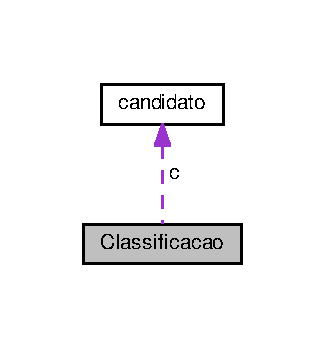
\includegraphics[width=156pt]{structClassificacao__coll__graph}
\end{center}
\end{figure}
\subsection*{Public Attributes}
\begin{DoxyCompactItemize}
\item 
\hyperlink{classcandidato}{candidato} $\ast$ \hyperlink{structClassificacao_a0d17a3011d8d230f262da09d271f66c5}{c}
\begin{DoxyCompactList}\small\item\em candidato \end{DoxyCompactList}\item 
float \hyperlink{structClassificacao_abe2dfdf576aadbd510980c17d337a1a9}{j1}
\begin{DoxyCompactList}\small\item\em pontuacao do jurado 1 \end{DoxyCompactList}\item 
float \hyperlink{structClassificacao_a1221d2875f866a4c9fea21f04888796a}{j2}
\begin{DoxyCompactList}\small\item\em pontuacao do jurado 2 \end{DoxyCompactList}\item 
float \hyperlink{structClassificacao_a3fd75e4d2503d5ecdb88814b808c6929}{j3}
\begin{DoxyCompactList}\small\item\em pontuacao do jurado 3 \end{DoxyCompactList}\item 
float \hyperlink{structClassificacao_a5f7d29ed16f73699cf485006bd333007}{media}
\begin{DoxyCompactList}\small\item\em resultado final \end{DoxyCompactList}\end{DoxyCompactItemize}


\subsection{Detailed Description}
contem a informacao das classificacoes obtidas por um candidato 

\subsection{Member Data Documentation}
\index{Classificacao@{Classificacao}!c@{c}}
\index{c@{c}!Classificacao@{Classificacao}}
\subsubsection[{\texorpdfstring{c}{c}}]{\setlength{\rightskip}{0pt plus 5cm}{\bf candidato}$\ast$ Classificacao\+::c}\hypertarget{structClassificacao_a0d17a3011d8d230f262da09d271f66c5}{}\label{structClassificacao_a0d17a3011d8d230f262da09d271f66c5}


candidato 

\index{Classificacao@{Classificacao}!j1@{j1}}
\index{j1@{j1}!Classificacao@{Classificacao}}
\subsubsection[{\texorpdfstring{j1}{j1}}]{\setlength{\rightskip}{0pt plus 5cm}float Classificacao\+::j1}\hypertarget{structClassificacao_abe2dfdf576aadbd510980c17d337a1a9}{}\label{structClassificacao_abe2dfdf576aadbd510980c17d337a1a9}


pontuacao do jurado 1 

\index{Classificacao@{Classificacao}!j2@{j2}}
\index{j2@{j2}!Classificacao@{Classificacao}}
\subsubsection[{\texorpdfstring{j2}{j2}}]{\setlength{\rightskip}{0pt plus 5cm}float Classificacao\+::j2}\hypertarget{structClassificacao_a1221d2875f866a4c9fea21f04888796a}{}\label{structClassificacao_a1221d2875f866a4c9fea21f04888796a}


pontuacao do jurado 2 

\index{Classificacao@{Classificacao}!j3@{j3}}
\index{j3@{j3}!Classificacao@{Classificacao}}
\subsubsection[{\texorpdfstring{j3}{j3}}]{\setlength{\rightskip}{0pt plus 5cm}float Classificacao\+::j3}\hypertarget{structClassificacao_a3fd75e4d2503d5ecdb88814b808c6929}{}\label{structClassificacao_a3fd75e4d2503d5ecdb88814b808c6929}


pontuacao do jurado 3 

\index{Classificacao@{Classificacao}!media@{media}}
\index{media@{media}!Classificacao@{Classificacao}}
\subsubsection[{\texorpdfstring{media}{media}}]{\setlength{\rightskip}{0pt plus 5cm}float Classificacao\+::media}\hypertarget{structClassificacao_a5f7d29ed16f73699cf485006bd333007}{}\label{structClassificacao_a5f7d29ed16f73699cf485006bd333007}


resultado final 



The documentation for this struct was generated from the following file\+:\begin{DoxyCompactItemize}
\item 
/home/amadeu/\+F\+E\+U\+P/\+A\+E\+D\+A\+\_\+\+Proj1/\hyperlink{fase_8h}{fase.\+h}\end{DoxyCompactItemize}

\hypertarget{structeq}{}\section{eq Struct Reference}
\label{structeq}\index{eq@{eq}}


{\ttfamily \#include $<$funcoes.\+h$>$}

\subsection*{Public Member Functions}
\begin{DoxyCompactItemize}
\item 
bool \hyperlink{structeq_a1e702c588ddf434e1b913636bf343911}{operator()} (const pair$<$ \hyperlink{classcandidato}{candidato}, string $>$ c1, const pair$<$ \hyperlink{classcandidato}{candidato}, string $>$ c2) const 
\end{DoxyCompactItemize}


\subsection{Member Function Documentation}
\index{eq@{eq}!operator()@{operator()}}
\index{operator()@{operator()}!eq@{eq}}
\subsubsection[{\texorpdfstring{operator()(const pair$<$ candidato, string $>$ c1, const pair$<$ candidato, string $>$ c2) const }{operator()(const pair< candidato, string > c1, const pair< candidato, string > c2) const }}]{\setlength{\rightskip}{0pt plus 5cm}bool eq\+::operator() (
\begin{DoxyParamCaption}
\item[{const pair$<$ {\bf candidato}, string $>$}]{c1, }
\item[{const pair$<$ {\bf candidato}, string $>$}]{c2}
\end{DoxyParamCaption}
) const\hspace{0.3cm}{\ttfamily [inline]}}\hypertarget{structeq_a1e702c588ddf434e1b913636bf343911}{}\label{structeq_a1e702c588ddf434e1b913636bf343911}


The documentation for this struct was generated from the following file\+:\begin{DoxyCompactItemize}
\item 
/home/amadeu/\+F\+E\+U\+P/\+A\+E\+D\+A\+\_\+\+Proj1/\hyperlink{funcoes_8h}{funcoes.\+h}\end{DoxyCompactItemize}

\hypertarget{classfase}{}\section{fase Class Reference}
\label{classfase}\index{fase@{fase}}


classe abstrata relativa as varia fases de uma sessao  




{\ttfamily \#include $<$fase.\+h$>$}



Inheritance diagram for fase\+:\nopagebreak
\begin{figure}[H]
\begin{center}
\leavevmode
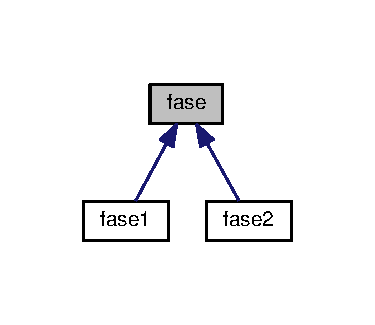
\includegraphics[width=180pt]{classfase__inherit__graph}
\end{center}
\end{figure}
\subsection*{Public Member Functions}
\begin{DoxyCompactItemize}
\item 
\hyperlink{classfase_aa083a44106dfc979915f9e9ffb78f206}{fase} ()
\begin{DoxyCompactList}\small\item\em construtor da classe fase \end{DoxyCompactList}\item 
virtual \hyperlink{classfase_a84ce4001850cdcf2c001feb38bc65a47}{$\sim$fase} ()
\begin{DoxyCompactList}\small\item\em destrutor da classe fase \end{DoxyCompactList}\item 
virtual void \hyperlink{classfase_af940cf6e1b3aaff1802f354d82d73208}{atribui\+Pontuacoes} ()=0
\begin{DoxyCompactList}\small\item\em metodo virtual para a atribuicao das pontuacoes numa fase \end{DoxyCompactList}\item 
virtual void \hyperlink{classfase_af0597909e632b43fb33f2b49f66280e1}{ordena\+Pontuacoes} ()=0
\begin{DoxyCompactList}\small\item\em metodo virtual para ordenar as classificacoes dos candidatos (da maior para a menor) \end{DoxyCompactList}\item 
virtual vector$<$ \hyperlink{structClassificacao}{Classificacao} $>$ \hyperlink{classfase_a44cb191d58429a075bd3820e847c2823}{get\+Classificacoes} () const =0
\begin{DoxyCompactList}\small\item\em metodo virtual que devolve as classificacoes dos candidatos duma certa fase \end{DoxyCompactList}\end{DoxyCompactItemize}


\subsection{Detailed Description}
classe abstrata relativa as varia fases de uma sessao 

\subsection{Constructor \& Destructor Documentation}
\index{fase@{fase}!fase@{fase}}
\index{fase@{fase}!fase@{fase}}
\subsubsection[{\texorpdfstring{fase()}{fase()}}]{\setlength{\rightskip}{0pt plus 5cm}fase\+::fase (
\begin{DoxyParamCaption}
{}
\end{DoxyParamCaption}
)}\hypertarget{classfase_aa083a44106dfc979915f9e9ffb78f206}{}\label{classfase_aa083a44106dfc979915f9e9ffb78f206}


construtor da classe fase 

\index{fase@{fase}!````~fase@{$\sim$fase}}
\index{````~fase@{$\sim$fase}!fase@{fase}}
\subsubsection[{\texorpdfstring{$\sim$fase()}{~fase()}}]{\setlength{\rightskip}{0pt plus 5cm}fase\+::$\sim$fase (
\begin{DoxyParamCaption}
{}
\end{DoxyParamCaption}
)\hspace{0.3cm}{\ttfamily [virtual]}}\hypertarget{classfase_a84ce4001850cdcf2c001feb38bc65a47}{}\label{classfase_a84ce4001850cdcf2c001feb38bc65a47}


destrutor da classe fase 



\subsection{Member Function Documentation}
\index{fase@{fase}!atribui\+Pontuacoes@{atribui\+Pontuacoes}}
\index{atribui\+Pontuacoes@{atribui\+Pontuacoes}!fase@{fase}}
\subsubsection[{\texorpdfstring{atribui\+Pontuacoes()=0}{atribuiPontuacoes()=0}}]{\setlength{\rightskip}{0pt plus 5cm}virtual void fase\+::atribui\+Pontuacoes (
\begin{DoxyParamCaption}
{}
\end{DoxyParamCaption}
)\hspace{0.3cm}{\ttfamily [pure virtual]}}\hypertarget{classfase_af940cf6e1b3aaff1802f354d82d73208}{}\label{classfase_af940cf6e1b3aaff1802f354d82d73208}


metodo virtual para a atribuicao das pontuacoes numa fase 



Implemented in \hyperlink{classfase2_a8088339c7740a9bdb0d26c270036a885}{fase2}, and \hyperlink{classfase1_ad4bd20d6f65510c72c6924cbd77b5af0}{fase1}.

\index{fase@{fase}!get\+Classificacoes@{get\+Classificacoes}}
\index{get\+Classificacoes@{get\+Classificacoes}!fase@{fase}}
\subsubsection[{\texorpdfstring{get\+Classificacoes() const =0}{getClassificacoes() const =0}}]{\setlength{\rightskip}{0pt plus 5cm}virtual vector$<${\bf Classificacao}$>$ fase\+::get\+Classificacoes (
\begin{DoxyParamCaption}
{}
\end{DoxyParamCaption}
) const\hspace{0.3cm}{\ttfamily [pure virtual]}}\hypertarget{classfase_a44cb191d58429a075bd3820e847c2823}{}\label{classfase_a44cb191d58429a075bd3820e847c2823}


metodo virtual que devolve as classificacoes dos candidatos duma certa fase 

\begin{DoxyReturn}{Returns}
vetor com as classificacoes 
\end{DoxyReturn}


Implemented in \hyperlink{classfase2_a9ce60146eeac9f5862e1eb5c87191418}{fase2}, and \hyperlink{classfase1_ab228229f675fb1581459b826f31d3d82}{fase1}.

\index{fase@{fase}!ordena\+Pontuacoes@{ordena\+Pontuacoes}}
\index{ordena\+Pontuacoes@{ordena\+Pontuacoes}!fase@{fase}}
\subsubsection[{\texorpdfstring{ordena\+Pontuacoes()=0}{ordenaPontuacoes()=0}}]{\setlength{\rightskip}{0pt plus 5cm}virtual void fase\+::ordena\+Pontuacoes (
\begin{DoxyParamCaption}
{}
\end{DoxyParamCaption}
)\hspace{0.3cm}{\ttfamily [pure virtual]}}\hypertarget{classfase_af0597909e632b43fb33f2b49f66280e1}{}\label{classfase_af0597909e632b43fb33f2b49f66280e1}


metodo virtual para ordenar as classificacoes dos candidatos (da maior para a menor) 



Implemented in \hyperlink{classfase2_a072c622b806ec59bedf3588a5886a153}{fase2}, and \hyperlink{classfase1_a630facb1c550249547876d73e2e9c2c9}{fase1}.



The documentation for this class was generated from the following files\+:\begin{DoxyCompactItemize}
\item 
/home/amadeu/\+F\+E\+U\+P/\+A\+E\+D\+A\+\_\+\+Proj1/\hyperlink{fase_8h}{fase.\+h}\item 
/home/amadeu/\+F\+E\+U\+P/\+A\+E\+D\+A\+\_\+\+Proj1/\hyperlink{fase_8cpp}{fase.\+cpp}\end{DoxyCompactItemize}

\hypertarget{classfase1}{}\section{fase1 Class Reference}
\label{classfase1}\index{fase1@{fase1}}


subclasse da classe fase relativa a primeira fase  




{\ttfamily \#include $<$fase.\+h$>$}



Inheritance diagram for fase1\+:\nopagebreak
\begin{figure}[H]
\begin{center}
\leavevmode
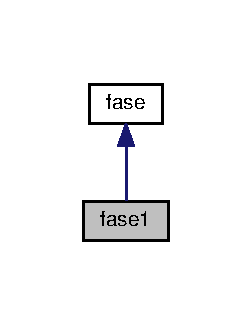
\includegraphics[width=121pt]{classfase1__inherit__graph}
\end{center}
\end{figure}


Collaboration diagram for fase1\+:\nopagebreak
\begin{figure}[H]
\begin{center}
\leavevmode
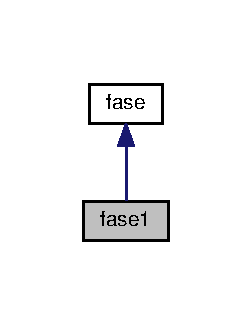
\includegraphics[width=121pt]{classfase1__coll__graph}
\end{center}
\end{figure}
\subsection*{Public Member Functions}
\begin{DoxyCompactItemize}
\item 
\hyperlink{classfase1_aa2bdac71181493e27b744862925c944b}{fase1} (\hyperlink{classsessao}{sessao} $\ast$s)
\begin{DoxyCompactList}\small\item\em construtor da class \hyperlink{classfase1}{fase1} \end{DoxyCompactList}\item 
\hyperlink{classfase1_a45c3a7c99c90a1c7079cf6045416b33c}{fase1} (string info)
\begin{DoxyCompactList}\small\item\em construtor da class \hyperlink{classfase1}{fase1} \end{DoxyCompactList}\item 
void \hyperlink{classfase1_ad4bd20d6f65510c72c6924cbd77b5af0}{atribui\+Pontuacoes} ()
\begin{DoxyCompactList}\small\item\em funcao para atribuir as pontuacoes de um candidato \end{DoxyCompactList}\item 
void \hyperlink{classfase1_a630facb1c550249547876d73e2e9c2c9}{ordena\+Pontuacoes} ()
\begin{DoxyCompactList}\small\item\em ordena as varias classificacoes de cada candidato de ordem decrescente tendo como base a media \end{DoxyCompactList}\item 
vector$<$ \hyperlink{structClassificacao}{Classificacao} $>$ \hyperlink{classfase1_ab228229f675fb1581459b826f31d3d82}{get\+Classificacoes} () const 
\begin{DoxyCompactList}\small\item\em devolve o vetor com as classificacoes \end{DoxyCompactList}\item 
\hyperlink{classsessao}{sessao} $\ast$ \hyperlink{classfase1_aa6e3c8314c055f90cec3b0a033e5b54e}{get\+Sessao} ()
\begin{DoxyCompactList}\small\item\em devolve a sessao correspondente a esta fase \end{DoxyCompactList}\end{DoxyCompactItemize}
\subsection*{Friends}
\begin{DoxyCompactItemize}
\item 
ostream \& \hyperlink{classfase1_a598506525641a0ba5d116c7d071e80a2}{operator$<$$<$} (ostream \&o, \hyperlink{classfase1}{fase1} f)
\begin{DoxyCompactList}\small\item\em overload do operador $<$$<$ para a classe \hyperlink{classfase1}{fase1} (ostream) \end{DoxyCompactList}\end{DoxyCompactItemize}


\subsection{Detailed Description}
subclasse da classe fase relativa a primeira fase 

\subsection{Constructor \& Destructor Documentation}
\index{fase1@{fase1}!fase1@{fase1}}
\index{fase1@{fase1}!fase1@{fase1}}
\subsubsection[{\texorpdfstring{fase1(sessao $\ast$s)}{fase1(sessao *s)}}]{\setlength{\rightskip}{0pt plus 5cm}fase1\+::fase1 (
\begin{DoxyParamCaption}
\item[{{\bf sessao} $\ast$}]{s}
\end{DoxyParamCaption}
)}\hypertarget{classfase1_aa2bdac71181493e27b744862925c944b}{}\label{classfase1_aa2bdac71181493e27b744862925c944b}


construtor da class \hyperlink{classfase1}{fase1} 


\begin{DoxyParams}{Parameters}
{\em s} & apontador para a sessao a que se pretende adicionar a primeira fase \\
\hline
\end{DoxyParams}
\index{fase1@{fase1}!fase1@{fase1}}
\index{fase1@{fase1}!fase1@{fase1}}
\subsubsection[{\texorpdfstring{fase1(string info)}{fase1(string info)}}]{\setlength{\rightskip}{0pt plus 5cm}fase1\+::fase1 (
\begin{DoxyParamCaption}
\item[{string}]{info}
\end{DoxyParamCaption}
)}\hypertarget{classfase1_a45c3a7c99c90a1c7079cf6045416b33c}{}\label{classfase1_a45c3a7c99c90a1c7079cf6045416b33c}


construtor da class \hyperlink{classfase1}{fase1} 


\begin{DoxyParams}{Parameters}
{\em info} & string com a informacao relativa à \hyperlink{classfase1}{fase1} \\
\hline
\end{DoxyParams}


\subsection{Member Function Documentation}
\index{fase1@{fase1}!atribui\+Pontuacoes@{atribui\+Pontuacoes}}
\index{atribui\+Pontuacoes@{atribui\+Pontuacoes}!fase1@{fase1}}
\subsubsection[{\texorpdfstring{atribui\+Pontuacoes()}{atribuiPontuacoes()}}]{\setlength{\rightskip}{0pt plus 5cm}void fase1\+::atribui\+Pontuacoes (
\begin{DoxyParamCaption}
{}
\end{DoxyParamCaption}
)\hspace{0.3cm}{\ttfamily [virtual]}}\hypertarget{classfase1_ad4bd20d6f65510c72c6924cbd77b5af0}{}\label{classfase1_ad4bd20d6f65510c72c6924cbd77b5af0}


funcao para atribuir as pontuacoes de um candidato 



Implements \hyperlink{classfase_af940cf6e1b3aaff1802f354d82d73208}{fase}.

\index{fase1@{fase1}!get\+Classificacoes@{get\+Classificacoes}}
\index{get\+Classificacoes@{get\+Classificacoes}!fase1@{fase1}}
\subsubsection[{\texorpdfstring{get\+Classificacoes() const }{getClassificacoes() const }}]{\setlength{\rightskip}{0pt plus 5cm}vector$<$ {\bf Classificacao} $>$ fase1\+::get\+Classificacoes (
\begin{DoxyParamCaption}
{}
\end{DoxyParamCaption}
) const\hspace{0.3cm}{\ttfamily [virtual]}}\hypertarget{classfase1_ab228229f675fb1581459b826f31d3d82}{}\label{classfase1_ab228229f675fb1581459b826f31d3d82}


devolve o vetor com as classificacoes 

\begin{DoxyReturn}{Returns}
vetor com classificacoes 
\end{DoxyReturn}


Implements \hyperlink{classfase_a44cb191d58429a075bd3820e847c2823}{fase}.

\index{fase1@{fase1}!get\+Sessao@{get\+Sessao}}
\index{get\+Sessao@{get\+Sessao}!fase1@{fase1}}
\subsubsection[{\texorpdfstring{get\+Sessao()}{getSessao()}}]{\setlength{\rightskip}{0pt plus 5cm}{\bf sessao} $\ast$ fase1\+::get\+Sessao (
\begin{DoxyParamCaption}
{}
\end{DoxyParamCaption}
)}\hypertarget{classfase1_aa6e3c8314c055f90cec3b0a033e5b54e}{}\label{classfase1_aa6e3c8314c055f90cec3b0a033e5b54e}


devolve a sessao correspondente a esta fase 

\begin{DoxyReturn}{Returns}
apontador para a sessa 
\end{DoxyReturn}
\index{fase1@{fase1}!ordena\+Pontuacoes@{ordena\+Pontuacoes}}
\index{ordena\+Pontuacoes@{ordena\+Pontuacoes}!fase1@{fase1}}
\subsubsection[{\texorpdfstring{ordena\+Pontuacoes()}{ordenaPontuacoes()}}]{\setlength{\rightskip}{0pt plus 5cm}void fase1\+::ordena\+Pontuacoes (
\begin{DoxyParamCaption}
{}
\end{DoxyParamCaption}
)\hspace{0.3cm}{\ttfamily [virtual]}}\hypertarget{classfase1_a630facb1c550249547876d73e2e9c2c9}{}\label{classfase1_a630facb1c550249547876d73e2e9c2c9}


ordena as varias classificacoes de cada candidato de ordem decrescente tendo como base a media 



Implements \hyperlink{classfase_af0597909e632b43fb33f2b49f66280e1}{fase}.



\subsection{Friends And Related Function Documentation}
\index{fase1@{fase1}!operator$<$$<$@{operator$<$$<$}}
\index{operator$<$$<$@{operator$<$$<$}!fase1@{fase1}}
\subsubsection[{\texorpdfstring{operator$<$$<$}{operator<<}}]{\setlength{\rightskip}{0pt plus 5cm}ostream\& operator$<$$<$ (
\begin{DoxyParamCaption}
\item[{ostream \&}]{o, }
\item[{{\bf fase1}}]{f}
\end{DoxyParamCaption}
)\hspace{0.3cm}{\ttfamily [friend]}}\hypertarget{classfase1_a598506525641a0ba5d116c7d071e80a2}{}\label{classfase1_a598506525641a0ba5d116c7d071e80a2}


overload do operador $<$$<$ para a classe \hyperlink{classfase1}{fase1} (ostream) 



The documentation for this class was generated from the following files\+:\begin{DoxyCompactItemize}
\item 
/home/amadeu/\+F\+E\+U\+P/\+A\+E\+D\+A\+\_\+\+Proj1/\hyperlink{fase_8h}{fase.\+h}\item 
/home/amadeu/\+F\+E\+U\+P/\+A\+E\+D\+A\+\_\+\+Proj1/\hyperlink{fase_8cpp}{fase.\+cpp}\end{DoxyCompactItemize}

\hypertarget{classfase2}{}\section{fase2 Class Reference}
\label{classfase2}\index{fase2@{fase2}}


subclasse da classe fase relativa a segunda fase  




{\ttfamily \#include $<$fase.\+h$>$}



Inheritance diagram for fase2\+:\nopagebreak
\begin{figure}[H]
\begin{center}
\leavevmode
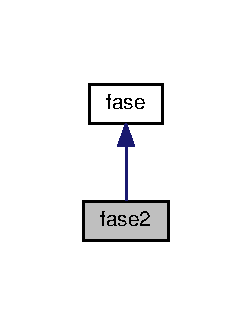
\includegraphics[width=121pt]{classfase2__inherit__graph}
\end{center}
\end{figure}


Collaboration diagram for fase2\+:\nopagebreak
\begin{figure}[H]
\begin{center}
\leavevmode
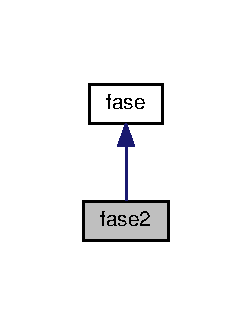
\includegraphics[width=121pt]{classfase2__coll__graph}
\end{center}
\end{figure}
\subsection*{Public Member Functions}
\begin{DoxyCompactItemize}
\item 
\hyperlink{classfase2_a35257f931f3c049ce109f8420a4947ce}{fase2} (\hyperlink{classfase1}{fase1} f, \hyperlink{classsessao}{sessao} $\ast$s)
\begin{DoxyCompactList}\small\item\em construtor da class \hyperlink{classfase2}{fase2} que passa a segunda fase os 5 melhores classificados da primeiara fase \end{DoxyCompactList}\item 
\hyperlink{classfase2_a50efc3d5d2b81385069e7db490088dd4}{fase2} (string info)
\begin{DoxyCompactList}\small\item\em construtor da class \hyperlink{classfase1}{fase1} \end{DoxyCompactList}\item 
void \hyperlink{classfase2_a072c622b806ec59bedf3588a5886a153}{ordena\+Pontuacoes} ()
\begin{DoxyCompactList}\small\item\em ordena as varias classificacoes de cada candidato de ordem decrescente tendo como base a media \end{DoxyCompactList}\item 
void \hyperlink{classfase2_a53f1281d38b661b21ec3954b41ea4945}{display\+Vencedor} ()
\begin{DoxyCompactList}\small\item\em funcao que da display do vencedor e da sua pontuacao \end{DoxyCompactList}\item 
void \hyperlink{classfase2_a8088339c7740a9bdb0d26c270036a885}{atribui\+Pontuacoes} ()
\begin{DoxyCompactList}\small\item\em funcao para atribuir as pontuacoes de um candidato \end{DoxyCompactList}\item 
vector$<$ \hyperlink{structClassificacao}{Classificacao} $>$ \hyperlink{classfase2_a9ce60146eeac9f5862e1eb5c87191418}{get\+Classificacoes} () const 
\begin{DoxyCompactList}\small\item\em devolve o vetor com as classificacoes \end{DoxyCompactList}\item 
\hyperlink{classsessao}{sessao} $\ast$ \hyperlink{classfase2_acef38bb05864322911031659dab18adf}{get\+Sessao} ()
\begin{DoxyCompactList}\small\item\em devolve a sessao correspondente a esta fase \end{DoxyCompactList}\end{DoxyCompactItemize}
\subsection*{Friends}
\begin{DoxyCompactItemize}
\item 
ostream \& \hyperlink{classfase2_a1fcb0da80eaeea4bf75c01e9472bd189}{operator$<$$<$} (ostream \&o, \hyperlink{classfase2}{fase2} f)
\begin{DoxyCompactList}\small\item\em overload do operador $<$$<$ para a classe \hyperlink{classfase2}{fase2} (ostream) \end{DoxyCompactList}\end{DoxyCompactItemize}


\subsection{Detailed Description}
subclasse da classe fase relativa a segunda fase 

\subsection{Constructor \& Destructor Documentation}
\index{fase2@{fase2}!fase2@{fase2}}
\index{fase2@{fase2}!fase2@{fase2}}
\subsubsection[{\texorpdfstring{fase2(fase1 f, sessao $\ast$s)}{fase2(fase1 f, sessao *s)}}]{\setlength{\rightskip}{0pt plus 5cm}fase2\+::fase2 (
\begin{DoxyParamCaption}
\item[{{\bf fase1}}]{f, }
\item[{{\bf sessao} $\ast$}]{s}
\end{DoxyParamCaption}
)}\hypertarget{classfase2_a35257f931f3c049ce109f8420a4947ce}{}\label{classfase2_a35257f931f3c049ce109f8420a4947ce}


construtor da class \hyperlink{classfase2}{fase2} que passa a segunda fase os 5 melhores classificados da primeiara fase 


\begin{DoxyParams}{Parameters}
{\em f} & primeirafase correspondente \\
\hline
{\em s} & apontador para a sessao a que se pretende adicionar a segunda fase \\
\hline
\end{DoxyParams}
\index{fase2@{fase2}!fase2@{fase2}}
\index{fase2@{fase2}!fase2@{fase2}}
\subsubsection[{\texorpdfstring{fase2(string info)}{fase2(string info)}}]{\setlength{\rightskip}{0pt plus 5cm}fase2\+::fase2 (
\begin{DoxyParamCaption}
\item[{string}]{info}
\end{DoxyParamCaption}
)}\hypertarget{classfase2_a50efc3d5d2b81385069e7db490088dd4}{}\label{classfase2_a50efc3d5d2b81385069e7db490088dd4}


construtor da class \hyperlink{classfase1}{fase1} 


\begin{DoxyParams}{Parameters}
{\em info} & string com a informacao relativa à \hyperlink{classfase1}{fase1} \\
\hline
\end{DoxyParams}


\subsection{Member Function Documentation}
\index{fase2@{fase2}!atribui\+Pontuacoes@{atribui\+Pontuacoes}}
\index{atribui\+Pontuacoes@{atribui\+Pontuacoes}!fase2@{fase2}}
\subsubsection[{\texorpdfstring{atribui\+Pontuacoes()}{atribuiPontuacoes()}}]{\setlength{\rightskip}{0pt plus 5cm}void fase2\+::atribui\+Pontuacoes (
\begin{DoxyParamCaption}
{}
\end{DoxyParamCaption}
)\hspace{0.3cm}{\ttfamily [virtual]}}\hypertarget{classfase2_a8088339c7740a9bdb0d26c270036a885}{}\label{classfase2_a8088339c7740a9bdb0d26c270036a885}


funcao para atribuir as pontuacoes de um candidato 



Implements \hyperlink{classfase_af940cf6e1b3aaff1802f354d82d73208}{fase}.

\index{fase2@{fase2}!display\+Vencedor@{display\+Vencedor}}
\index{display\+Vencedor@{display\+Vencedor}!fase2@{fase2}}
\subsubsection[{\texorpdfstring{display\+Vencedor()}{displayVencedor()}}]{\setlength{\rightskip}{0pt plus 5cm}void fase2\+::display\+Vencedor (
\begin{DoxyParamCaption}
{}
\end{DoxyParamCaption}
)}\hypertarget{classfase2_a53f1281d38b661b21ec3954b41ea4945}{}\label{classfase2_a53f1281d38b661b21ec3954b41ea4945}


funcao que da display do vencedor e da sua pontuacao 

\index{fase2@{fase2}!get\+Classificacoes@{get\+Classificacoes}}
\index{get\+Classificacoes@{get\+Classificacoes}!fase2@{fase2}}
\subsubsection[{\texorpdfstring{get\+Classificacoes() const }{getClassificacoes() const }}]{\setlength{\rightskip}{0pt plus 5cm}vector$<$ {\bf Classificacao} $>$ fase2\+::get\+Classificacoes (
\begin{DoxyParamCaption}
{}
\end{DoxyParamCaption}
) const\hspace{0.3cm}{\ttfamily [virtual]}}\hypertarget{classfase2_a9ce60146eeac9f5862e1eb5c87191418}{}\label{classfase2_a9ce60146eeac9f5862e1eb5c87191418}


devolve o vetor com as classificacoes 

\begin{DoxyReturn}{Returns}
vetor com classificacoes 
\end{DoxyReturn}


Implements \hyperlink{classfase_a44cb191d58429a075bd3820e847c2823}{fase}.

\index{fase2@{fase2}!get\+Sessao@{get\+Sessao}}
\index{get\+Sessao@{get\+Sessao}!fase2@{fase2}}
\subsubsection[{\texorpdfstring{get\+Sessao()}{getSessao()}}]{\setlength{\rightskip}{0pt plus 5cm}{\bf sessao} $\ast$ fase2\+::get\+Sessao (
\begin{DoxyParamCaption}
{}
\end{DoxyParamCaption}
)}\hypertarget{classfase2_acef38bb05864322911031659dab18adf}{}\label{classfase2_acef38bb05864322911031659dab18adf}


devolve a sessao correspondente a esta fase 

\begin{DoxyReturn}{Returns}
apontador para a sessa 
\end{DoxyReturn}
\index{fase2@{fase2}!ordena\+Pontuacoes@{ordena\+Pontuacoes}}
\index{ordena\+Pontuacoes@{ordena\+Pontuacoes}!fase2@{fase2}}
\subsubsection[{\texorpdfstring{ordena\+Pontuacoes()}{ordenaPontuacoes()}}]{\setlength{\rightskip}{0pt plus 5cm}void fase2\+::ordena\+Pontuacoes (
\begin{DoxyParamCaption}
{}
\end{DoxyParamCaption}
)\hspace{0.3cm}{\ttfamily [virtual]}}\hypertarget{classfase2_a072c622b806ec59bedf3588a5886a153}{}\label{classfase2_a072c622b806ec59bedf3588a5886a153}


ordena as varias classificacoes de cada candidato de ordem decrescente tendo como base a media 



Implements \hyperlink{classfase_af0597909e632b43fb33f2b49f66280e1}{fase}.



\subsection{Friends And Related Function Documentation}
\index{fase2@{fase2}!operator$<$$<$@{operator$<$$<$}}
\index{operator$<$$<$@{operator$<$$<$}!fase2@{fase2}}
\subsubsection[{\texorpdfstring{operator$<$$<$}{operator<<}}]{\setlength{\rightskip}{0pt plus 5cm}ostream\& operator$<$$<$ (
\begin{DoxyParamCaption}
\item[{ostream \&}]{o, }
\item[{{\bf fase2}}]{f}
\end{DoxyParamCaption}
)\hspace{0.3cm}{\ttfamily [friend]}}\hypertarget{classfase2_a1fcb0da80eaeea4bf75c01e9472bd189}{}\label{classfase2_a1fcb0da80eaeea4bf75c01e9472bd189}


overload do operador $<$$<$ para a classe \hyperlink{classfase2}{fase2} (ostream) 



The documentation for this class was generated from the following files\+:\begin{DoxyCompactItemize}
\item 
/home/amadeu/\+F\+E\+U\+P/\+A\+E\+D\+A\+\_\+\+Proj1/\hyperlink{fase_8h}{fase.\+h}\item 
/home/amadeu/\+F\+E\+U\+P/\+A\+E\+D\+A\+\_\+\+Proj1/\hyperlink{fase_8cpp}{fase.\+cpp}\end{DoxyCompactItemize}

\hypertarget{structh}{}\section{h Struct Reference}
\label{structh}\index{h@{h}}


{\ttfamily \#include $<$funcoes.\+h$>$}

\subsection*{Public Member Functions}
\begin{DoxyCompactItemize}
\item 
int \hyperlink{structh_aa20e9aecdf5d33f41788047b33e8a1b3}{operator()} (const pair$<$ \hyperlink{classcandidato}{candidato}, string $>$ c) const 
\end{DoxyCompactItemize}


\subsection{Member Function Documentation}
\index{h@{h}!operator()@{operator()}}
\index{operator()@{operator()}!h@{h}}
\subsubsection[{\texorpdfstring{operator()(const pair$<$ candidato, string $>$ c) const }{operator()(const pair< candidato, string > c) const }}]{\setlength{\rightskip}{0pt plus 5cm}int h\+::operator() (
\begin{DoxyParamCaption}
\item[{const pair$<$ {\bf candidato}, string $>$}]{c}
\end{DoxyParamCaption}
) const\hspace{0.3cm}{\ttfamily [inline]}}\hypertarget{structh_aa20e9aecdf5d33f41788047b33e8a1b3}{}\label{structh_aa20e9aecdf5d33f41788047b33e8a1b3}


The documentation for this struct was generated from the following file\+:\begin{DoxyCompactItemize}
\item 
/home/amadeu/\+F\+E\+U\+P/\+A\+E\+D\+A\+\_\+\+Proj1/\hyperlink{funcoes_8h}{funcoes.\+h}\end{DoxyCompactItemize}

\hypertarget{classjurado}{}\section{jurado Class Reference}
\label{classjurado}\index{jurado@{jurado}}


classe com as informacoes relativas a um jurado  




{\ttfamily \#include $<$jurado.\+h$>$}

\subsection*{Public Member Functions}
\begin{DoxyCompactItemize}
\item 
\hyperlink{classjurado_a9677e0aa464ceeb5b7ad73c6425f5aba}{jurado} ()
\begin{DoxyCompactList}\small\item\em construtor de um objecto da class jurado \end{DoxyCompactList}\item 
\hyperlink{classjurado_ac1743fdba044e673ef7d572763d3d23a}{jurado} (string nome, string morada, string telemovel, string arte)
\begin{DoxyCompactList}\small\item\em construtor de um objecto da class jurado \end{DoxyCompactList}\item 
\hyperlink{classjurado_a5e43e7112be419c57122dba488de3b46}{jurado} (string info)
\begin{DoxyCompactList}\small\item\em construtor de um objeto da class jurado \end{DoxyCompactList}\item 
\hyperlink{classjurado_abe6cb3aaffde689138379457ea881fa7}{$\sim$jurado} ()
\begin{DoxyCompactList}\small\item\em destrutor de um objecto da class jurado \end{DoxyCompactList}\item 
void \hyperlink{classjurado_a017b6f4965237e7bf8009a1bdbead43b}{set\+Nome} (string nome)
\begin{DoxyCompactList}\small\item\em funcao que altera o nome do jurado \end{DoxyCompactList}\item 
void \hyperlink{classjurado_a8dbe8d5f9d9d4bcc03c5e074068d98a7}{set\+Morada} (string morada)
\begin{DoxyCompactList}\small\item\em funcao que altera a morada do jurado \end{DoxyCompactList}\item 
void \hyperlink{classjurado_abb5ebbc58c0dc5379e47673d4695ac70}{set\+Telemovel} (string telemovel)
\begin{DoxyCompactList}\small\item\em funcao que altera o telemovel do jurado \end{DoxyCompactList}\item 
void \hyperlink{classjurado_a8e33ffaa864e0cbb645e65e0b571d000}{set\+Arte} (string arte)
\begin{DoxyCompactList}\small\item\em funcao que altera a arte do jurado \end{DoxyCompactList}\item 
string \hyperlink{classjurado_a02bb9270bf2d86644017814317546456}{get\+Nome} () const 
\begin{DoxyCompactList}\small\item\em funcao que devolve o nome do jurado \end{DoxyCompactList}\item 
string \hyperlink{classjurado_ac5843b1f1e60196e5fa4697c5e6c897a}{get\+Morada} () const 
\begin{DoxyCompactList}\small\item\em funcao que devolve a morada do jurado \end{DoxyCompactList}\item 
string \hyperlink{classjurado_aa48845847fcb0cf892c0f324ca95934f}{get\+Telemovel} () const 
\begin{DoxyCompactList}\small\item\em funcao que devolve o numero de telemovel do jurado \end{DoxyCompactList}\item 
string \hyperlink{classjurado_a300946cb2a34dec4b688d76a002c6e3f}{get\+Arte} () const 
\begin{DoxyCompactList}\small\item\em funcao que devolve a arte do jurado \end{DoxyCompactList}\item 
vector$<$ \hyperlink{classsessao}{sessao} $\ast$ $>$ \hyperlink{classjurado_a3bc8171a54abd5d01413fa12fb3b388a}{get\+Sessoes} () const 
\begin{DoxyCompactList}\small\item\em funcao que devolve as sessoes do jurado \end{DoxyCompactList}\item 
void \hyperlink{classjurado_af6a351dce6c2e9dac755254bc4137b58}{set\+Sessoes} (vector$<$ \hyperlink{classsessao}{sessao} $\ast$ $>$ s)
\begin{DoxyCompactList}\small\item\em funcao que adiciona as sessoes ao jurado \end{DoxyCompactList}\item 
void \hyperlink{classjurado_a3c18c6b03f81ac8927571f9008307ab7}{adiciona\+Sessao} (\hyperlink{classsessao}{sessao} $\ast$s)
\begin{DoxyCompactList}\small\item\em funcao que adiciona uma sessao às sessoes ao jurado \end{DoxyCompactList}\item 
void \hyperlink{classjurado_adb3bd37bd370642bcdc4c8cb404ff9de}{remove\+Sessao} (\hyperlink{classsessao}{sessao} $\ast$s)
\begin{DoxyCompactList}\small\item\em funcao que remove uma sessao das sessoes do jurado \end{DoxyCompactList}\item 
bool \hyperlink{classjurado_a2cd7669a1f16ebe8cb1ac997dd82f8cc}{jurado\+Ocupado} (vector$<$ int $>$ data)
\begin{DoxyCompactList}\small\item\em verifica se o jurado ja tem alguma sessao naquele dia \end{DoxyCompactList}\end{DoxyCompactItemize}
\subsection*{Friends}
\begin{DoxyCompactItemize}
\item 
ostream \& \hyperlink{classjurado_afbbe037345e49122dbab2fd21278225d}{operator$<$$<$} (ostream \&o, const \hyperlink{classjurado}{jurado} $\ast$j)
\begin{DoxyCompactList}\small\item\em overload do operador $<$$<$ para a classe jurado (ostream) \end{DoxyCompactList}\item 
ofstream \& \hyperlink{classjurado_a9778784aa84765cf798f6cfc59656ce2}{operator$<$$<$} (ofstream \&o, const \hyperlink{classjurado}{jurado} $\ast$j)
\begin{DoxyCompactList}\small\item\em overload do operador $<$$<$ para a classe jurado (fstream) \end{DoxyCompactList}\end{DoxyCompactItemize}


\subsection{Detailed Description}
classe com as informacoes relativas a um jurado 

\subsection{Constructor \& Destructor Documentation}
\index{jurado@{jurado}!jurado@{jurado}}
\index{jurado@{jurado}!jurado@{jurado}}
\subsubsection[{\texorpdfstring{jurado()}{jurado()}}]{\setlength{\rightskip}{0pt plus 5cm}jurado\+::jurado (
\begin{DoxyParamCaption}
{}
\end{DoxyParamCaption}
)}\hypertarget{classjurado_a9677e0aa464ceeb5b7ad73c6425f5aba}{}\label{classjurado_a9677e0aa464ceeb5b7ad73c6425f5aba}


construtor de um objecto da class jurado 

\index{jurado@{jurado}!jurado@{jurado}}
\index{jurado@{jurado}!jurado@{jurado}}
\subsubsection[{\texorpdfstring{jurado(string nome, string morada, string telemovel, string arte)}{jurado(string nome, string morada, string telemovel, string arte)}}]{\setlength{\rightskip}{0pt plus 5cm}jurado\+::jurado (
\begin{DoxyParamCaption}
\item[{string}]{nome, }
\item[{string}]{morada, }
\item[{string}]{telemovel, }
\item[{string}]{arte}
\end{DoxyParamCaption}
)}\hypertarget{classjurado_ac1743fdba044e673ef7d572763d3d23a}{}\label{classjurado_ac1743fdba044e673ef7d572763d3d23a}


construtor de um objecto da class jurado 


\begin{DoxyParams}{Parameters}
{\em nome} & nome do jurado \\
\hline
{\em morada} & morada do jurado \\
\hline
{\em telemovel} & telemovel do jurado \\
\hline
{\em arte} & arte em que o jurado e especialista \\
\hline
\end{DoxyParams}
\index{jurado@{jurado}!jurado@{jurado}}
\index{jurado@{jurado}!jurado@{jurado}}
\subsubsection[{\texorpdfstring{jurado(string info)}{jurado(string info)}}]{\setlength{\rightskip}{0pt plus 5cm}jurado\+::jurado (
\begin{DoxyParamCaption}
\item[{string}]{info}
\end{DoxyParamCaption}
)}\hypertarget{classjurado_a5e43e7112be419c57122dba488de3b46}{}\label{classjurado_a5e43e7112be419c57122dba488de3b46}


construtor de um objeto da class jurado 


\begin{DoxyParams}{Parameters}
{\em info} & string com a informacao toda de um jurado \\
\hline
\end{DoxyParams}
\index{jurado@{jurado}!````~jurado@{$\sim$jurado}}
\index{````~jurado@{$\sim$jurado}!jurado@{jurado}}
\subsubsection[{\texorpdfstring{$\sim$jurado()}{~jurado()}}]{\setlength{\rightskip}{0pt plus 5cm}jurado\+::$\sim$jurado (
\begin{DoxyParamCaption}
{}
\end{DoxyParamCaption}
)}\hypertarget{classjurado_abe6cb3aaffde689138379457ea881fa7}{}\label{classjurado_abe6cb3aaffde689138379457ea881fa7}


destrutor de um objecto da class jurado 



\subsection{Member Function Documentation}
\index{jurado@{jurado}!adiciona\+Sessao@{adiciona\+Sessao}}
\index{adiciona\+Sessao@{adiciona\+Sessao}!jurado@{jurado}}
\subsubsection[{\texorpdfstring{adiciona\+Sessao(sessao $\ast$s)}{adicionaSessao(sessao *s)}}]{\setlength{\rightskip}{0pt plus 5cm}void jurado\+::adiciona\+Sessao (
\begin{DoxyParamCaption}
\item[{{\bf sessao} $\ast$}]{s}
\end{DoxyParamCaption}
)}\hypertarget{classjurado_a3c18c6b03f81ac8927571f9008307ab7}{}\label{classjurado_a3c18c6b03f81ac8927571f9008307ab7}


funcao que adiciona uma sessao às sessoes ao jurado 


\begin{DoxyParams}{Parameters}
{\em s} & sessao a adicionar \\
\hline
\end{DoxyParams}
\index{jurado@{jurado}!get\+Arte@{get\+Arte}}
\index{get\+Arte@{get\+Arte}!jurado@{jurado}}
\subsubsection[{\texorpdfstring{get\+Arte() const }{getArte() const }}]{\setlength{\rightskip}{0pt plus 5cm}string jurado\+::get\+Arte (
\begin{DoxyParamCaption}
{}
\end{DoxyParamCaption}
) const}\hypertarget{classjurado_a300946cb2a34dec4b688d76a002c6e3f}{}\label{classjurado_a300946cb2a34dec4b688d76a002c6e3f}


funcao que devolve a arte do jurado 

\begin{DoxyReturn}{Returns}
arte do jurado 
\end{DoxyReturn}
\index{jurado@{jurado}!get\+Morada@{get\+Morada}}
\index{get\+Morada@{get\+Morada}!jurado@{jurado}}
\subsubsection[{\texorpdfstring{get\+Morada() const }{getMorada() const }}]{\setlength{\rightskip}{0pt plus 5cm}string jurado\+::get\+Morada (
\begin{DoxyParamCaption}
{}
\end{DoxyParamCaption}
) const}\hypertarget{classjurado_ac5843b1f1e60196e5fa4697c5e6c897a}{}\label{classjurado_ac5843b1f1e60196e5fa4697c5e6c897a}


funcao que devolve a morada do jurado 

\begin{DoxyReturn}{Returns}
morada do jurado 
\end{DoxyReturn}
\index{jurado@{jurado}!get\+Nome@{get\+Nome}}
\index{get\+Nome@{get\+Nome}!jurado@{jurado}}
\subsubsection[{\texorpdfstring{get\+Nome() const }{getNome() const }}]{\setlength{\rightskip}{0pt plus 5cm}string jurado\+::get\+Nome (
\begin{DoxyParamCaption}
{}
\end{DoxyParamCaption}
) const}\hypertarget{classjurado_a02bb9270bf2d86644017814317546456}{}\label{classjurado_a02bb9270bf2d86644017814317546456}


funcao que devolve o nome do jurado 

\begin{DoxyReturn}{Returns}
nome do jurado 
\end{DoxyReturn}
\index{jurado@{jurado}!get\+Sessoes@{get\+Sessoes}}
\index{get\+Sessoes@{get\+Sessoes}!jurado@{jurado}}
\subsubsection[{\texorpdfstring{get\+Sessoes() const }{getSessoes() const }}]{\setlength{\rightskip}{0pt plus 5cm}vector$<$ {\bf sessao} $\ast$ $>$ jurado\+::get\+Sessoes (
\begin{DoxyParamCaption}
{}
\end{DoxyParamCaption}
) const}\hypertarget{classjurado_a3bc8171a54abd5d01413fa12fb3b388a}{}\label{classjurado_a3bc8171a54abd5d01413fa12fb3b388a}


funcao que devolve as sessoes do jurado 

\begin{DoxyReturn}{Returns}
sessoes do jurado 
\end{DoxyReturn}
\index{jurado@{jurado}!get\+Telemovel@{get\+Telemovel}}
\index{get\+Telemovel@{get\+Telemovel}!jurado@{jurado}}
\subsubsection[{\texorpdfstring{get\+Telemovel() const }{getTelemovel() const }}]{\setlength{\rightskip}{0pt plus 5cm}string jurado\+::get\+Telemovel (
\begin{DoxyParamCaption}
{}
\end{DoxyParamCaption}
) const}\hypertarget{classjurado_aa48845847fcb0cf892c0f324ca95934f}{}\label{classjurado_aa48845847fcb0cf892c0f324ca95934f}


funcao que devolve o numero de telemovel do jurado 

\begin{DoxyReturn}{Returns}
telemovel do jurado 
\end{DoxyReturn}
\index{jurado@{jurado}!jurado\+Ocupado@{jurado\+Ocupado}}
\index{jurado\+Ocupado@{jurado\+Ocupado}!jurado@{jurado}}
\subsubsection[{\texorpdfstring{jurado\+Ocupado(vector$<$ int $>$ data)}{juradoOcupado(vector< int > data)}}]{\setlength{\rightskip}{0pt plus 5cm}bool jurado\+::jurado\+Ocupado (
\begin{DoxyParamCaption}
\item[{vector$<$ int $>$}]{data}
\end{DoxyParamCaption}
)}\hypertarget{classjurado_a2cd7669a1f16ebe8cb1ac997dd82f8cc}{}\label{classjurado_a2cd7669a1f16ebe8cb1ac997dd82f8cc}


verifica se o jurado ja tem alguma sessao naquele dia 

\begin{DoxyReturn}{Returns}
true se sim, false se nao; 
\end{DoxyReturn}
\index{jurado@{jurado}!remove\+Sessao@{remove\+Sessao}}
\index{remove\+Sessao@{remove\+Sessao}!jurado@{jurado}}
\subsubsection[{\texorpdfstring{remove\+Sessao(sessao $\ast$s)}{removeSessao(sessao *s)}}]{\setlength{\rightskip}{0pt plus 5cm}void jurado\+::remove\+Sessao (
\begin{DoxyParamCaption}
\item[{{\bf sessao} $\ast$}]{s}
\end{DoxyParamCaption}
)}\hypertarget{classjurado_adb3bd37bd370642bcdc4c8cb404ff9de}{}\label{classjurado_adb3bd37bd370642bcdc4c8cb404ff9de}


funcao que remove uma sessao das sessoes do jurado 


\begin{DoxyParams}{Parameters}
{\em s} & sessao a remover \\
\hline
\end{DoxyParams}
\index{jurado@{jurado}!set\+Arte@{set\+Arte}}
\index{set\+Arte@{set\+Arte}!jurado@{jurado}}
\subsubsection[{\texorpdfstring{set\+Arte(string arte)}{setArte(string arte)}}]{\setlength{\rightskip}{0pt plus 5cm}void jurado\+::set\+Arte (
\begin{DoxyParamCaption}
\item[{string}]{arte}
\end{DoxyParamCaption}
)}\hypertarget{classjurado_a8e33ffaa864e0cbb645e65e0b571d000}{}\label{classjurado_a8e33ffaa864e0cbb645e65e0b571d000}


funcao que altera a arte do jurado 


\begin{DoxyParams}{Parameters}
{\em arte} & arte do jurado \\
\hline
\end{DoxyParams}
\index{jurado@{jurado}!set\+Morada@{set\+Morada}}
\index{set\+Morada@{set\+Morada}!jurado@{jurado}}
\subsubsection[{\texorpdfstring{set\+Morada(string morada)}{setMorada(string morada)}}]{\setlength{\rightskip}{0pt plus 5cm}void jurado\+::set\+Morada (
\begin{DoxyParamCaption}
\item[{string}]{morada}
\end{DoxyParamCaption}
)}\hypertarget{classjurado_a8dbe8d5f9d9d4bcc03c5e074068d98a7}{}\label{classjurado_a8dbe8d5f9d9d4bcc03c5e074068d98a7}


funcao que altera a morada do jurado 


\begin{DoxyParams}{Parameters}
{\em morada} & morada do jurado \\
\hline
\end{DoxyParams}
\index{jurado@{jurado}!set\+Nome@{set\+Nome}}
\index{set\+Nome@{set\+Nome}!jurado@{jurado}}
\subsubsection[{\texorpdfstring{set\+Nome(string nome)}{setNome(string nome)}}]{\setlength{\rightskip}{0pt plus 5cm}void jurado\+::set\+Nome (
\begin{DoxyParamCaption}
\item[{string}]{nome}
\end{DoxyParamCaption}
)}\hypertarget{classjurado_a017b6f4965237e7bf8009a1bdbead43b}{}\label{classjurado_a017b6f4965237e7bf8009a1bdbead43b}


funcao que altera o nome do jurado 


\begin{DoxyParams}{Parameters}
{\em nome} & nome do jurado \\
\hline
\end{DoxyParams}
\index{jurado@{jurado}!set\+Sessoes@{set\+Sessoes}}
\index{set\+Sessoes@{set\+Sessoes}!jurado@{jurado}}
\subsubsection[{\texorpdfstring{set\+Sessoes(vector$<$ sessao $\ast$ $>$ s)}{setSessoes(vector< sessao * > s)}}]{\setlength{\rightskip}{0pt plus 5cm}void jurado\+::set\+Sessoes (
\begin{DoxyParamCaption}
\item[{vector$<$ {\bf sessao} $\ast$ $>$}]{s}
\end{DoxyParamCaption}
)}\hypertarget{classjurado_af6a351dce6c2e9dac755254bc4137b58}{}\label{classjurado_af6a351dce6c2e9dac755254bc4137b58}


funcao que adiciona as sessoes ao jurado 


\begin{DoxyParams}{Parameters}
{\em s} & vetor de sessoes a adicionar \\
\hline
\end{DoxyParams}
\index{jurado@{jurado}!set\+Telemovel@{set\+Telemovel}}
\index{set\+Telemovel@{set\+Telemovel}!jurado@{jurado}}
\subsubsection[{\texorpdfstring{set\+Telemovel(string telemovel)}{setTelemovel(string telemovel)}}]{\setlength{\rightskip}{0pt plus 5cm}void jurado\+::set\+Telemovel (
\begin{DoxyParamCaption}
\item[{string}]{telemovel}
\end{DoxyParamCaption}
)}\hypertarget{classjurado_abb5ebbc58c0dc5379e47673d4695ac70}{}\label{classjurado_abb5ebbc58c0dc5379e47673d4695ac70}


funcao que altera o telemovel do jurado 


\begin{DoxyParams}{Parameters}
{\em telemovel} & telemovel do jurado \\
\hline
\end{DoxyParams}


\subsection{Friends And Related Function Documentation}
\index{jurado@{jurado}!operator$<$$<$@{operator$<$$<$}}
\index{operator$<$$<$@{operator$<$$<$}!jurado@{jurado}}
\subsubsection[{\texorpdfstring{operator$<$$<$}{operator<<}}]{\setlength{\rightskip}{0pt plus 5cm}ostream\& operator$<$$<$ (
\begin{DoxyParamCaption}
\item[{ostream \&}]{o, }
\item[{const {\bf jurado} $\ast$}]{j}
\end{DoxyParamCaption}
)\hspace{0.3cm}{\ttfamily [friend]}}\hypertarget{classjurado_afbbe037345e49122dbab2fd21278225d}{}\label{classjurado_afbbe037345e49122dbab2fd21278225d}


overload do operador $<$$<$ para a classe jurado (ostream) 

\index{jurado@{jurado}!operator$<$$<$@{operator$<$$<$}}
\index{operator$<$$<$@{operator$<$$<$}!jurado@{jurado}}
\subsubsection[{\texorpdfstring{operator$<$$<$}{operator<<}}]{\setlength{\rightskip}{0pt plus 5cm}ofstream\& operator$<$$<$ (
\begin{DoxyParamCaption}
\item[{ofstream \&}]{o, }
\item[{const {\bf jurado} $\ast$}]{j}
\end{DoxyParamCaption}
)\hspace{0.3cm}{\ttfamily [friend]}}\hypertarget{classjurado_a9778784aa84765cf798f6cfc59656ce2}{}\label{classjurado_a9778784aa84765cf798f6cfc59656ce2}


overload do operador $<$$<$ para a classe jurado (fstream) 



The documentation for this class was generated from the following files\+:\begin{DoxyCompactItemize}
\item 
/home/amadeu/\+F\+E\+U\+P/\+A\+E\+D\+A\+\_\+\+Proj1/\hyperlink{jurado_8h}{jurado.\+h}\item 
/home/amadeu/\+F\+E\+U\+P/\+A\+E\+D\+A\+\_\+\+Proj1/\hyperlink{jurado_8cpp}{jurado.\+cpp}\end{DoxyCompactItemize}

\hypertarget{classJuradoJaExiste}{}\section{Jurado\+Ja\+Existe Class Reference}
\label{classJuradoJaExiste}\index{Jurado\+Ja\+Existe@{Jurado\+Ja\+Existe}}


excepcao para quando um objeto da classe jurado ja existe  




{\ttfamily \#include $<$jurado.\+h$>$}

\subsection*{Public Member Functions}
\begin{DoxyCompactItemize}
\item 
\hyperlink{classJuradoJaExiste_a079c17599ccb15515eadac4af3d07cf4}{Jurado\+Ja\+Existe} (string \hyperlink{classJuradoJaExiste_a3f471f626f78a0c2d57b7e1f445c300e}{nome})
\begin{DoxyCompactList}\small\item\em constructor da excepcao \hyperlink{classJuradoJaExiste}{Jurado\+Ja\+Existe} \end{DoxyCompactList}\end{DoxyCompactItemize}
\subsection*{Public Attributes}
\begin{DoxyCompactItemize}
\item 
string \hyperlink{classJuradoJaExiste_a3f471f626f78a0c2d57b7e1f445c300e}{nome}
\begin{DoxyCompactList}\small\item\em nome do jurado \end{DoxyCompactList}\end{DoxyCompactItemize}


\subsection{Detailed Description}
excepcao para quando um objeto da classe jurado ja existe 

\subsection{Constructor \& Destructor Documentation}
\index{Jurado\+Ja\+Existe@{Jurado\+Ja\+Existe}!Jurado\+Ja\+Existe@{Jurado\+Ja\+Existe}}
\index{Jurado\+Ja\+Existe@{Jurado\+Ja\+Existe}!Jurado\+Ja\+Existe@{Jurado\+Ja\+Existe}}
\subsubsection[{\texorpdfstring{Jurado\+Ja\+Existe(string nome)}{JuradoJaExiste(string nome)}}]{\setlength{\rightskip}{0pt plus 5cm}Jurado\+Ja\+Existe\+::\+Jurado\+Ja\+Existe (
\begin{DoxyParamCaption}
\item[{string}]{nome}
\end{DoxyParamCaption}
)\hspace{0.3cm}{\ttfamily [inline]}}\hypertarget{classJuradoJaExiste_a079c17599ccb15515eadac4af3d07cf4}{}\label{classJuradoJaExiste_a079c17599ccb15515eadac4af3d07cf4}


constructor da excepcao \hyperlink{classJuradoJaExiste}{Jurado\+Ja\+Existe} 


\begin{DoxyParams}{Parameters}
{\em nome} & nome do jurado \\
\hline
\end{DoxyParams}


\subsection{Member Data Documentation}
\index{Jurado\+Ja\+Existe@{Jurado\+Ja\+Existe}!nome@{nome}}
\index{nome@{nome}!Jurado\+Ja\+Existe@{Jurado\+Ja\+Existe}}
\subsubsection[{\texorpdfstring{nome}{nome}}]{\setlength{\rightskip}{0pt plus 5cm}string Jurado\+Ja\+Existe\+::nome}\hypertarget{classJuradoJaExiste_a3f471f626f78a0c2d57b7e1f445c300e}{}\label{classJuradoJaExiste_a3f471f626f78a0c2d57b7e1f445c300e}


nome do jurado 



The documentation for this class was generated from the following file\+:\begin{DoxyCompactItemize}
\item 
/home/amadeu/\+F\+E\+U\+P/\+A\+E\+D\+A\+\_\+\+Proj1/\hyperlink{jurado_8h}{jurado.\+h}\end{DoxyCompactItemize}

\hypertarget{classJuradoNaoExiste}{}\section{Jurado\+Nao\+Existe Class Reference}
\label{classJuradoNaoExiste}\index{Jurado\+Nao\+Existe@{Jurado\+Nao\+Existe}}


excepcao para quando um objeto da classe jurado nao existe  




{\ttfamily \#include $<$jurado.\+h$>$}

\subsection*{Public Member Functions}
\begin{DoxyCompactItemize}
\item 
\hyperlink{classJuradoNaoExiste_a6eb6f183981cb6ce86961e775b7dd8b4}{Jurado\+Nao\+Existe} (string \hyperlink{classJuradoNaoExiste_ac87a8a650e0a9a791687aef1ddc2add2}{nome})
\begin{DoxyCompactList}\small\item\em constructor da excepcao \hyperlink{classJuradoNaoExiste}{Jurado\+Nao\+Existe} \end{DoxyCompactList}\end{DoxyCompactItemize}
\subsection*{Public Attributes}
\begin{DoxyCompactItemize}
\item 
string \hyperlink{classJuradoNaoExiste_ac87a8a650e0a9a791687aef1ddc2add2}{nome}
\begin{DoxyCompactList}\small\item\em nome do jurado \end{DoxyCompactList}\end{DoxyCompactItemize}


\subsection{Detailed Description}
excepcao para quando um objeto da classe jurado nao existe 

\subsection{Constructor \& Destructor Documentation}
\index{Jurado\+Nao\+Existe@{Jurado\+Nao\+Existe}!Jurado\+Nao\+Existe@{Jurado\+Nao\+Existe}}
\index{Jurado\+Nao\+Existe@{Jurado\+Nao\+Existe}!Jurado\+Nao\+Existe@{Jurado\+Nao\+Existe}}
\subsubsection[{\texorpdfstring{Jurado\+Nao\+Existe(string nome)}{JuradoNaoExiste(string nome)}}]{\setlength{\rightskip}{0pt plus 5cm}Jurado\+Nao\+Existe\+::\+Jurado\+Nao\+Existe (
\begin{DoxyParamCaption}
\item[{string}]{nome}
\end{DoxyParamCaption}
)\hspace{0.3cm}{\ttfamily [inline]}}\hypertarget{classJuradoNaoExiste_a6eb6f183981cb6ce86961e775b7dd8b4}{}\label{classJuradoNaoExiste_a6eb6f183981cb6ce86961e775b7dd8b4}


constructor da excepcao \hyperlink{classJuradoNaoExiste}{Jurado\+Nao\+Existe} 


\begin{DoxyParams}{Parameters}
{\em nome} & nome do jurado \\
\hline
\end{DoxyParams}


\subsection{Member Data Documentation}
\index{Jurado\+Nao\+Existe@{Jurado\+Nao\+Existe}!nome@{nome}}
\index{nome@{nome}!Jurado\+Nao\+Existe@{Jurado\+Nao\+Existe}}
\subsubsection[{\texorpdfstring{nome}{nome}}]{\setlength{\rightskip}{0pt plus 5cm}string Jurado\+Nao\+Existe\+::nome}\hypertarget{classJuradoNaoExiste_ac87a8a650e0a9a791687aef1ddc2add2}{}\label{classJuradoNaoExiste_ac87a8a650e0a9a791687aef1ddc2add2}


nome do jurado 



The documentation for this class was generated from the following file\+:\begin{DoxyCompactItemize}
\item 
/home/amadeu/\+F\+E\+U\+P/\+A\+E\+D\+A\+\_\+\+Proj1/\hyperlink{jurado_8h}{jurado.\+h}\end{DoxyCompactItemize}

\hypertarget{classjuradoOcupado}{}\section{jurado\+Ocupado Class Reference}
\label{classjuradoOcupado}\index{jurado\+Ocupado@{jurado\+Ocupado}}


excepcao para quando um objeto da classe jurado ja se encontra ocupado num determinado dia  




{\ttfamily \#include $<$jurado.\+h$>$}

\subsection*{Public Member Functions}
\begin{DoxyCompactItemize}
\item 
\hyperlink{classjuradoOcupado_af6fa48b520c4cae1fa64edb9f590669e}{jurado\+Ocupado} (string \hyperlink{classjuradoOcupado_a38fa76168b435d63e7eb6294a644793e}{nome}, vector$<$ int $>$ \hyperlink{classjuradoOcupado_aceeab32c1cf0547045ba7166491d566a}{data})
\begin{DoxyCompactList}\small\item\em constructor da excepcao \hyperlink{classjuradoOcupado}{jurado\+Ocupado} \end{DoxyCompactList}\end{DoxyCompactItemize}
\subsection*{Public Attributes}
\begin{DoxyCompactItemize}
\item 
string \hyperlink{classjuradoOcupado_a38fa76168b435d63e7eb6294a644793e}{nome}
\begin{DoxyCompactList}\small\item\em nome do jurado \end{DoxyCompactList}\item 
vector$<$ int $>$ \hyperlink{classjuradoOcupado_aceeab32c1cf0547045ba7166491d566a}{data}
\begin{DoxyCompactList}\small\item\em data em que este esta ocupado \end{DoxyCompactList}\end{DoxyCompactItemize}


\subsection{Detailed Description}
excepcao para quando um objeto da classe jurado ja se encontra ocupado num determinado dia 

\subsection{Constructor \& Destructor Documentation}
\index{jurado\+Ocupado@{jurado\+Ocupado}!jurado\+Ocupado@{jurado\+Ocupado}}
\index{jurado\+Ocupado@{jurado\+Ocupado}!jurado\+Ocupado@{jurado\+Ocupado}}
\subsubsection[{\texorpdfstring{jurado\+Ocupado(string nome, vector$<$ int $>$ data)}{juradoOcupado(string nome, vector< int > data)}}]{\setlength{\rightskip}{0pt plus 5cm}jurado\+Ocupado\+::jurado\+Ocupado (
\begin{DoxyParamCaption}
\item[{string}]{nome, }
\item[{vector$<$ int $>$}]{data}
\end{DoxyParamCaption}
)\hspace{0.3cm}{\ttfamily [inline]}}\hypertarget{classjuradoOcupado_af6fa48b520c4cae1fa64edb9f590669e}{}\label{classjuradoOcupado_af6fa48b520c4cae1fa64edb9f590669e}


constructor da excepcao \hyperlink{classjuradoOcupado}{jurado\+Ocupado} 


\begin{DoxyParams}{Parameters}
{\em nome} & nome do jurado \\
\hline
{\em data} & data em que esta ocupado \\
\hline
\end{DoxyParams}


\subsection{Member Data Documentation}
\index{jurado\+Ocupado@{jurado\+Ocupado}!data@{data}}
\index{data@{data}!jurado\+Ocupado@{jurado\+Ocupado}}
\subsubsection[{\texorpdfstring{data}{data}}]{\setlength{\rightskip}{0pt plus 5cm}vector$<$int$>$ jurado\+Ocupado\+::data}\hypertarget{classjuradoOcupado_aceeab32c1cf0547045ba7166491d566a}{}\label{classjuradoOcupado_aceeab32c1cf0547045ba7166491d566a}


data em que este esta ocupado 

\index{jurado\+Ocupado@{jurado\+Ocupado}!nome@{nome}}
\index{nome@{nome}!jurado\+Ocupado@{jurado\+Ocupado}}
\subsubsection[{\texorpdfstring{nome}{nome}}]{\setlength{\rightskip}{0pt plus 5cm}string jurado\+Ocupado\+::nome}\hypertarget{classjuradoOcupado_a38fa76168b435d63e7eb6294a644793e}{}\label{classjuradoOcupado_a38fa76168b435d63e7eb6294a644793e}


nome do jurado 



The documentation for this class was generated from the following file\+:\begin{DoxyCompactItemize}
\item 
/home/amadeu/\+F\+E\+U\+P/\+A\+E\+D\+A\+\_\+\+Proj1/\hyperlink{jurado_8h}{jurado.\+h}\end{DoxyCompactItemize}

\hypertarget{classsessao}{}\section{sessao Class Reference}
\label{classsessao}\index{sessao@{sessao}}


classe com as informacoes relativas a uma sessao  




{\ttfamily \#include $<$sessao.\+h$>$}

\subsection*{Public Member Functions}
\begin{DoxyCompactItemize}
\item 
\hyperlink{classsessao_aeffd6315e32e04d53e0ae43b531bf185}{sessao} ()
\begin{DoxyCompactList}\small\item\em constructor da class sessao (inicializa dia mes e ano a zero) \end{DoxyCompactList}\item 
\hyperlink{classsessao_aa0c4f133563230ae0f975a3214134362}{$\sim$sessao} ()
\begin{DoxyCompactList}\small\item\em destrutor da class sessao \end{DoxyCompactList}\item 
\hyperlink{classsessao_af1c11649ff608dbc4d51e5189be9cec5}{sessao} (string info)
\begin{DoxyCompactList}\small\item\em construtor da class sessao \end{DoxyCompactList}\item 
\hyperlink{classsessao_a289b712ee7876adb7a838796e9bd5cb3}{sessao} (string genero\+Arte, vector$<$ int $>$ data)
\begin{DoxyCompactList}\small\item\em constructor da class sessao \end{DoxyCompactList}\item 
void \hyperlink{classsessao_a0924c2db7776396e07bdfe9e0f39d05f}{set\+Arte} (string genero\+Arte)
\begin{DoxyCompactList}\small\item\em altera o genero de arte da sessao \end{DoxyCompactList}\item 
void \hyperlink{classsessao_ad9af167622260d3b9804d926aade4249}{set\+Concluida} (bool c)
\begin{DoxyCompactList}\small\item\em altera se a sessao ja foi concluida \end{DoxyCompactList}\item 
void \hyperlink{classsessao_a7c9a1eaba24458e7b70053cc0d9f6dc4}{set\+Data} (vector$<$ int $>$ data)
\begin{DoxyCompactList}\small\item\em altera data da sessao \end{DoxyCompactList}\item 
void \hyperlink{classsessao_a1802bcff6720bf14b6387ef9d7943f6c}{set\+Candidatos} (vector$<$ \hyperlink{classcandidato}{candidato} $\ast$ $>$ c)
\begin{DoxyCompactList}\small\item\em altera o vetor de candidatos \end{DoxyCompactList}\item 
vector$<$ int $>$ \hyperlink{classsessao_aa9da748eb3886e40295893379ac500fd}{get\+Data} () const 
\begin{DoxyCompactList}\small\item\em funcao que devolve num array a data(dia, mes, ano) \end{DoxyCompactList}\item 
string \hyperlink{classsessao_a31a5d1fe361cab689d81f4fd96baae91}{get\+Genero\+Arte} () const 
\begin{DoxyCompactList}\small\item\em funcao que devolve o genero de arte de uma sessao \end{DoxyCompactList}\item 
vector$<$ \hyperlink{classcandidato}{candidato} $\ast$ $>$ \hyperlink{classsessao_aaeb774f071377658f957f909d29bf0c8}{get\+Candidatos} () const 
\begin{DoxyCompactList}\small\item\em funcao que devolve os candidatos de uma sessao \end{DoxyCompactList}\item 
vector$<$ \hyperlink{classjurado}{jurado} $\ast$ $>$ \hyperlink{classsessao_a6e384ba6e74b654bee58ccff5ed241fe}{get\+Jurados} () const 
\begin{DoxyCompactList}\small\item\em funcao que devolve os jurados de uma sessao \end{DoxyCompactList}\item 
void \hyperlink{classsessao_a48c51d6f1f2f8c948a0a227336de1d12}{adiciona\+Candidato} (\hyperlink{classcandidato}{candidato} $\ast$c)
\begin{DoxyCompactList}\small\item\em adiciona um candidato a sessao \end{DoxyCompactList}\item 
void \hyperlink{classsessao_a0eee24076fd8c1e474e1868abb9d166d}{adiciona\+Jurado} (\hyperlink{classjurado}{jurado} $\ast$j)
\begin{DoxyCompactList}\small\item\em adiciona um jurado a sessao \end{DoxyCompactList}\item 
int \hyperlink{classsessao_a247360575defbe2733ed6293a6d90a0d}{get\+Numero\+Jurados} () const 
\begin{DoxyCompactList}\small\item\em diz quantos jurados tem a sessao \end{DoxyCompactList}\item 
bool \hyperlink{classsessao_ab9e1e5203a930bcbf8ec4233972e6676}{sessao\+Concluida} () const 
\begin{DoxyCompactList}\small\item\em diz se a sessao ja for concluida \end{DoxyCompactList}\item 
bool \hyperlink{classsessao_ac7da1ba482dc3a5b65f4ad3915a2420e}{operator$<$} (const \hyperlink{classsessao}{sessao} $\ast$\&s) const 
\begin{DoxyCompactList}\small\item\em overload do operador $<$ para a classe sessao \end{DoxyCompactList}\end{DoxyCompactItemize}
\subsection*{Friends}
\begin{DoxyCompactItemize}
\item 
ostream \& \hyperlink{classsessao_a442be9403858cf93de76510cccc64496}{operator$<$$<$} (ostream \&o, const \hyperlink{classsessao}{sessao} $\ast$s)
\begin{DoxyCompactList}\small\item\em overload do operador $<$$<$ para a classe sessao (ostream) \end{DoxyCompactList}\item 
ofstream \& \hyperlink{classsessao_ac46d6bce5998eb1597ae5866c39938c5}{operator$<$$<$} (ofstream \&o, const \hyperlink{classsessao}{sessao} $\ast$s)
\begin{DoxyCompactList}\small\item\em overload do operador $<$$<$ para a classe sessao (fstream) \end{DoxyCompactList}\end{DoxyCompactItemize}


\subsection{Detailed Description}
classe com as informacoes relativas a uma sessao 

\subsection{Constructor \& Destructor Documentation}
\index{sessao@{sessao}!sessao@{sessao}}
\index{sessao@{sessao}!sessao@{sessao}}
\subsubsection[{\texorpdfstring{sessao()}{sessao()}}]{\setlength{\rightskip}{0pt plus 5cm}sessao\+::sessao (
\begin{DoxyParamCaption}
{}
\end{DoxyParamCaption}
)}\hypertarget{classsessao_aeffd6315e32e04d53e0ae43b531bf185}{}\label{classsessao_aeffd6315e32e04d53e0ae43b531bf185}


constructor da class sessao (inicializa dia mes e ano a zero) 

\index{sessao@{sessao}!````~sessao@{$\sim$sessao}}
\index{````~sessao@{$\sim$sessao}!sessao@{sessao}}
\subsubsection[{\texorpdfstring{$\sim$sessao()}{~sessao()}}]{\setlength{\rightskip}{0pt plus 5cm}sessao\+::$\sim$sessao (
\begin{DoxyParamCaption}
{}
\end{DoxyParamCaption}
)}\hypertarget{classsessao_aa0c4f133563230ae0f975a3214134362}{}\label{classsessao_aa0c4f133563230ae0f975a3214134362}


destrutor da class sessao 

\index{sessao@{sessao}!sessao@{sessao}}
\index{sessao@{sessao}!sessao@{sessao}}
\subsubsection[{\texorpdfstring{sessao(string info)}{sessao(string info)}}]{\setlength{\rightskip}{0pt plus 5cm}sessao\+::sessao (
\begin{DoxyParamCaption}
\item[{string}]{info}
\end{DoxyParamCaption}
)}\hypertarget{classsessao_af1c11649ff608dbc4d51e5189be9cec5}{}\label{classsessao_af1c11649ff608dbc4d51e5189be9cec5}


construtor da class sessao 


\begin{DoxyParams}{Parameters}
{\em info} & string com toda a informacao acerca de uma sessao \\
\hline
\end{DoxyParams}
\index{sessao@{sessao}!sessao@{sessao}}
\index{sessao@{sessao}!sessao@{sessao}}
\subsubsection[{\texorpdfstring{sessao(string genero\+Arte, vector$<$ int $>$ data)}{sessao(string generoArte, vector< int > data)}}]{\setlength{\rightskip}{0pt plus 5cm}sessao\+::sessao (
\begin{DoxyParamCaption}
\item[{string}]{genero\+Arte, }
\item[{vector$<$ int $>$}]{data}
\end{DoxyParamCaption}
)}\hypertarget{classsessao_a289b712ee7876adb7a838796e9bd5cb3}{}\label{classsessao_a289b712ee7876adb7a838796e9bd5cb3}


constructor da class sessao 


\begin{DoxyParams}{Parameters}
{\em genero\+Arte} & genero de arte da sessao \\
\hline
{\em data} & dia,mes,ano da sessao ,respetivamente \\
\hline
\end{DoxyParams}


\subsection{Member Function Documentation}
\index{sessao@{sessao}!adiciona\+Candidato@{adiciona\+Candidato}}
\index{adiciona\+Candidato@{adiciona\+Candidato}!sessao@{sessao}}
\subsubsection[{\texorpdfstring{adiciona\+Candidato(candidato $\ast$c)}{adicionaCandidato(candidato *c)}}]{\setlength{\rightskip}{0pt plus 5cm}void sessao\+::adiciona\+Candidato (
\begin{DoxyParamCaption}
\item[{{\bf candidato} $\ast$}]{c}
\end{DoxyParamCaption}
)}\hypertarget{classsessao_a48c51d6f1f2f8c948a0a227336de1d12}{}\label{classsessao_a48c51d6f1f2f8c948a0a227336de1d12}


adiciona um candidato a sessao 


\begin{DoxyParams}{Parameters}
{\em c} & candidato a adicionar \\
\hline
\end{DoxyParams}
\index{sessao@{sessao}!adiciona\+Jurado@{adiciona\+Jurado}}
\index{adiciona\+Jurado@{adiciona\+Jurado}!sessao@{sessao}}
\subsubsection[{\texorpdfstring{adiciona\+Jurado(jurado $\ast$j)}{adicionaJurado(jurado *j)}}]{\setlength{\rightskip}{0pt plus 5cm}void sessao\+::adiciona\+Jurado (
\begin{DoxyParamCaption}
\item[{{\bf jurado} $\ast$}]{j}
\end{DoxyParamCaption}
)}\hypertarget{classsessao_a0eee24076fd8c1e474e1868abb9d166d}{}\label{classsessao_a0eee24076fd8c1e474e1868abb9d166d}


adiciona um jurado a sessao 


\begin{DoxyParams}{Parameters}
{\em j} & jurado a adicionar \\
\hline
\end{DoxyParams}
\index{sessao@{sessao}!get\+Candidatos@{get\+Candidatos}}
\index{get\+Candidatos@{get\+Candidatos}!sessao@{sessao}}
\subsubsection[{\texorpdfstring{get\+Candidatos() const }{getCandidatos() const }}]{\setlength{\rightskip}{0pt plus 5cm}vector$<$ {\bf candidato} $\ast$ $>$ sessao\+::get\+Candidatos (
\begin{DoxyParamCaption}
{}
\end{DoxyParamCaption}
) const}\hypertarget{classsessao_aaeb774f071377658f957f909d29bf0c8}{}\label{classsessao_aaeb774f071377658f957f909d29bf0c8}


funcao que devolve os candidatos de uma sessao 

\begin{DoxyReturn}{Returns}
candidatos da sessao 
\end{DoxyReturn}
\index{sessao@{sessao}!get\+Data@{get\+Data}}
\index{get\+Data@{get\+Data}!sessao@{sessao}}
\subsubsection[{\texorpdfstring{get\+Data() const }{getData() const }}]{\setlength{\rightskip}{0pt plus 5cm}vector$<$ int $>$ sessao\+::get\+Data (
\begin{DoxyParamCaption}
{}
\end{DoxyParamCaption}
) const}\hypertarget{classsessao_aa9da748eb3886e40295893379ac500fd}{}\label{classsessao_aa9da748eb3886e40295893379ac500fd}


funcao que devolve num array a data(dia, mes, ano) 

\begin{DoxyReturn}{Returns}
vetor de int\textquotesingle{}s com a data 
\end{DoxyReturn}
\index{sessao@{sessao}!get\+Genero\+Arte@{get\+Genero\+Arte}}
\index{get\+Genero\+Arte@{get\+Genero\+Arte}!sessao@{sessao}}
\subsubsection[{\texorpdfstring{get\+Genero\+Arte() const }{getGeneroArte() const }}]{\setlength{\rightskip}{0pt plus 5cm}string sessao\+::get\+Genero\+Arte (
\begin{DoxyParamCaption}
{}
\end{DoxyParamCaption}
) const}\hypertarget{classsessao_a31a5d1fe361cab689d81f4fd96baae91}{}\label{classsessao_a31a5d1fe361cab689d81f4fd96baae91}


funcao que devolve o genero de arte de uma sessao 

\begin{DoxyReturn}{Returns}
genero\+Arte da sessao 
\end{DoxyReturn}
\index{sessao@{sessao}!get\+Jurados@{get\+Jurados}}
\index{get\+Jurados@{get\+Jurados}!sessao@{sessao}}
\subsubsection[{\texorpdfstring{get\+Jurados() const }{getJurados() const }}]{\setlength{\rightskip}{0pt plus 5cm}vector$<$ {\bf jurado} $\ast$ $>$ sessao\+::get\+Jurados (
\begin{DoxyParamCaption}
{}
\end{DoxyParamCaption}
) const}\hypertarget{classsessao_a6e384ba6e74b654bee58ccff5ed241fe}{}\label{classsessao_a6e384ba6e74b654bee58ccff5ed241fe}


funcao que devolve os jurados de uma sessao 

\begin{DoxyReturn}{Returns}
jurados da sessao 
\end{DoxyReturn}
\index{sessao@{sessao}!get\+Numero\+Jurados@{get\+Numero\+Jurados}}
\index{get\+Numero\+Jurados@{get\+Numero\+Jurados}!sessao@{sessao}}
\subsubsection[{\texorpdfstring{get\+Numero\+Jurados() const }{getNumeroJurados() const }}]{\setlength{\rightskip}{0pt plus 5cm}int sessao\+::get\+Numero\+Jurados (
\begin{DoxyParamCaption}
{}
\end{DoxyParamCaption}
) const}\hypertarget{classsessao_a247360575defbe2733ed6293a6d90a0d}{}\label{classsessao_a247360575defbe2733ed6293a6d90a0d}


diz quantos jurados tem a sessao 

\begin{DoxyReturn}{Returns}
numero de jurados 
\end{DoxyReturn}
\index{sessao@{sessao}!operator$<$@{operator$<$}}
\index{operator$<$@{operator$<$}!sessao@{sessao}}
\subsubsection[{\texorpdfstring{operator$<$(const sessao $\ast$\&s) const }{operator<(const sessao *&s) const }}]{\setlength{\rightskip}{0pt plus 5cm}bool sessao\+::operator$<$ (
\begin{DoxyParamCaption}
\item[{const {\bf sessao} $\ast$\&}]{s}
\end{DoxyParamCaption}
) const}\hypertarget{classsessao_ac7da1ba482dc3a5b65f4ad3915a2420e}{}\label{classsessao_ac7da1ba482dc3a5b65f4ad3915a2420e}


overload do operador $<$ para a classe sessao 

\index{sessao@{sessao}!sessao\+Concluida@{sessao\+Concluida}}
\index{sessao\+Concluida@{sessao\+Concluida}!sessao@{sessao}}
\subsubsection[{\texorpdfstring{sessao\+Concluida() const }{sessaoConcluida() const }}]{\setlength{\rightskip}{0pt plus 5cm}bool sessao\+::sessao\+Concluida (
\begin{DoxyParamCaption}
{}
\end{DoxyParamCaption}
) const}\hypertarget{classsessao_ab9e1e5203a930bcbf8ec4233972e6676}{}\label{classsessao_ab9e1e5203a930bcbf8ec4233972e6676}


diz se a sessao ja for concluida 

\begin{DoxyReturn}{Returns}
valor da variavel concluida 
\end{DoxyReturn}
\index{sessao@{sessao}!set\+Arte@{set\+Arte}}
\index{set\+Arte@{set\+Arte}!sessao@{sessao}}
\subsubsection[{\texorpdfstring{set\+Arte(string genero\+Arte)}{setArte(string generoArte)}}]{\setlength{\rightskip}{0pt plus 5cm}void sessao\+::set\+Arte (
\begin{DoxyParamCaption}
\item[{string}]{genero\+Arte}
\end{DoxyParamCaption}
)}\hypertarget{classsessao_a0924c2db7776396e07bdfe9e0f39d05f}{}\label{classsessao_a0924c2db7776396e07bdfe9e0f39d05f}


altera o genero de arte da sessao 


\begin{DoxyParams}{Parameters}
{\em genero\+Arte} & generto de arte da sessao \\
\hline
\end{DoxyParams}
\index{sessao@{sessao}!set\+Candidatos@{set\+Candidatos}}
\index{set\+Candidatos@{set\+Candidatos}!sessao@{sessao}}
\subsubsection[{\texorpdfstring{set\+Candidatos(vector$<$ candidato $\ast$ $>$ c)}{setCandidatos(vector< candidato * > c)}}]{\setlength{\rightskip}{0pt plus 5cm}void sessao\+::set\+Candidatos (
\begin{DoxyParamCaption}
\item[{vector$<$ {\bf candidato} $\ast$ $>$}]{c}
\end{DoxyParamCaption}
)}\hypertarget{classsessao_a1802bcff6720bf14b6387ef9d7943f6c}{}\label{classsessao_a1802bcff6720bf14b6387ef9d7943f6c}


altera o vetor de candidatos 


\begin{DoxyParams}{Parameters}
{\em c} & novo vetor de candidatos \\
\hline
\end{DoxyParams}
\index{sessao@{sessao}!set\+Concluida@{set\+Concluida}}
\index{set\+Concluida@{set\+Concluida}!sessao@{sessao}}
\subsubsection[{\texorpdfstring{set\+Concluida(bool c)}{setConcluida(bool c)}}]{\setlength{\rightskip}{0pt plus 5cm}void sessao\+::set\+Concluida (
\begin{DoxyParamCaption}
\item[{bool}]{c}
\end{DoxyParamCaption}
)}\hypertarget{classsessao_ad9af167622260d3b9804d926aade4249}{}\label{classsessao_ad9af167622260d3b9804d926aade4249}


altera se a sessao ja foi concluida 


\begin{DoxyParams}{Parameters}
{\em c} & valor para alterar \\
\hline
\end{DoxyParams}
\index{sessao@{sessao}!set\+Data@{set\+Data}}
\index{set\+Data@{set\+Data}!sessao@{sessao}}
\subsubsection[{\texorpdfstring{set\+Data(vector$<$ int $>$ data)}{setData(vector< int > data)}}]{\setlength{\rightskip}{0pt plus 5cm}void sessao\+::set\+Data (
\begin{DoxyParamCaption}
\item[{vector$<$ int $>$}]{data}
\end{DoxyParamCaption}
)}\hypertarget{classsessao_a7c9a1eaba24458e7b70053cc0d9f6dc4}{}\label{classsessao_a7c9a1eaba24458e7b70053cc0d9f6dc4}


altera data da sessao 


\begin{DoxyParams}{Parameters}
{\em data} & vetor com dia mes e ano para alterar \\
\hline
\end{DoxyParams}


\subsection{Friends And Related Function Documentation}
\index{sessao@{sessao}!operator$<$$<$@{operator$<$$<$}}
\index{operator$<$$<$@{operator$<$$<$}!sessao@{sessao}}
\subsubsection[{\texorpdfstring{operator$<$$<$}{operator<<}}]{\setlength{\rightskip}{0pt plus 5cm}ostream\& operator$<$$<$ (
\begin{DoxyParamCaption}
\item[{ostream \&}]{o, }
\item[{const {\bf sessao} $\ast$}]{s}
\end{DoxyParamCaption}
)\hspace{0.3cm}{\ttfamily [friend]}}\hypertarget{classsessao_a442be9403858cf93de76510cccc64496}{}\label{classsessao_a442be9403858cf93de76510cccc64496}


overload do operador $<$$<$ para a classe sessao (ostream) 

\index{sessao@{sessao}!operator$<$$<$@{operator$<$$<$}}
\index{operator$<$$<$@{operator$<$$<$}!sessao@{sessao}}
\subsubsection[{\texorpdfstring{operator$<$$<$}{operator<<}}]{\setlength{\rightskip}{0pt plus 5cm}ofstream\& operator$<$$<$ (
\begin{DoxyParamCaption}
\item[{ofstream \&}]{o, }
\item[{const {\bf sessao} $\ast$}]{s}
\end{DoxyParamCaption}
)\hspace{0.3cm}{\ttfamily [friend]}}\hypertarget{classsessao_ac46d6bce5998eb1597ae5866c39938c5}{}\label{classsessao_ac46d6bce5998eb1597ae5866c39938c5}


overload do operador $<$$<$ para a classe sessao (fstream) 



The documentation for this class was generated from the following files\+:\begin{DoxyCompactItemize}
\item 
/home/amadeu/\+F\+E\+U\+P/\+A\+E\+D\+A\+\_\+\+Proj1/\hyperlink{sessao_8h}{sessao.\+h}\item 
/home/amadeu/\+F\+E\+U\+P/\+A\+E\+D\+A\+\_\+\+Proj1/\hyperlink{sessao_8cpp}{sessao.\+cpp}\end{DoxyCompactItemize}

\hypertarget{classsessaoJaExiste}{}\section{sessao\+Ja\+Existe Class Reference}
\label{classsessaoJaExiste}\index{sessao\+Ja\+Existe@{sessao\+Ja\+Existe}}


excepcao para quando um objeto da classe sessao ja existe  




{\ttfamily \#include $<$sessao.\+h$>$}

\subsection*{Public Member Functions}
\begin{DoxyCompactItemize}
\item 
\hyperlink{classsessaoJaExiste_a0d90110fbef005844d1d711a7103ada2}{sessao\+Ja\+Existe} (string \hyperlink{classsessaoJaExiste_a9f0e4f38a0f1cebabdb28aa888e29dd2}{genero\+Arte}, vector$<$ int $>$ \hyperlink{classsessaoJaExiste_a7d8d84328e2b2dbd00336712d3341825}{data})
\begin{DoxyCompactList}\small\item\em constructor da excepcao \hyperlink{classsessaoJaExiste}{sessao\+Ja\+Existe} \end{DoxyCompactList}\end{DoxyCompactItemize}
\subsection*{Public Attributes}
\begin{DoxyCompactItemize}
\item 
string \hyperlink{classsessaoJaExiste_a9f0e4f38a0f1cebabdb28aa888e29dd2}{genero\+Arte}
\begin{DoxyCompactList}\small\item\em genero de arte da sessao \end{DoxyCompactList}\item 
vector$<$ int $>$ \hyperlink{classsessaoJaExiste_a7d8d84328e2b2dbd00336712d3341825}{data}
\begin{DoxyCompactList}\small\item\em data da sessao \end{DoxyCompactList}\end{DoxyCompactItemize}


\subsection{Detailed Description}
excepcao para quando um objeto da classe sessao ja existe 

\subsection{Constructor \& Destructor Documentation}
\index{sessao\+Ja\+Existe@{sessao\+Ja\+Existe}!sessao\+Ja\+Existe@{sessao\+Ja\+Existe}}
\index{sessao\+Ja\+Existe@{sessao\+Ja\+Existe}!sessao\+Ja\+Existe@{sessao\+Ja\+Existe}}
\subsubsection[{\texorpdfstring{sessao\+Ja\+Existe(string genero\+Arte, vector$<$ int $>$ data)}{sessaoJaExiste(string generoArte, vector< int > data)}}]{\setlength{\rightskip}{0pt plus 5cm}sessao\+Ja\+Existe\+::sessao\+Ja\+Existe (
\begin{DoxyParamCaption}
\item[{string}]{genero\+Arte, }
\item[{vector$<$ int $>$}]{data}
\end{DoxyParamCaption}
)\hspace{0.3cm}{\ttfamily [inline]}}\hypertarget{classsessaoJaExiste_a0d90110fbef005844d1d711a7103ada2}{}\label{classsessaoJaExiste_a0d90110fbef005844d1d711a7103ada2}


constructor da excepcao \hyperlink{classsessaoJaExiste}{sessao\+Ja\+Existe} 


\begin{DoxyParams}{Parameters}
{\em genero\+Arte} & genero de arte da sessao; \\
\hline
{\em data} & vetor com data(dia,mes,ano) da sessao; \\
\hline
\end{DoxyParams}


\subsection{Member Data Documentation}
\index{sessao\+Ja\+Existe@{sessao\+Ja\+Existe}!data@{data}}
\index{data@{data}!sessao\+Ja\+Existe@{sessao\+Ja\+Existe}}
\subsubsection[{\texorpdfstring{data}{data}}]{\setlength{\rightskip}{0pt plus 5cm}vector$<$int$>$ sessao\+Ja\+Existe\+::data}\hypertarget{classsessaoJaExiste_a7d8d84328e2b2dbd00336712d3341825}{}\label{classsessaoJaExiste_a7d8d84328e2b2dbd00336712d3341825}


data da sessao 

\index{sessao\+Ja\+Existe@{sessao\+Ja\+Existe}!genero\+Arte@{genero\+Arte}}
\index{genero\+Arte@{genero\+Arte}!sessao\+Ja\+Existe@{sessao\+Ja\+Existe}}
\subsubsection[{\texorpdfstring{genero\+Arte}{generoArte}}]{\setlength{\rightskip}{0pt plus 5cm}string sessao\+Ja\+Existe\+::genero\+Arte}\hypertarget{classsessaoJaExiste_a9f0e4f38a0f1cebabdb28aa888e29dd2}{}\label{classsessaoJaExiste_a9f0e4f38a0f1cebabdb28aa888e29dd2}


genero de arte da sessao 



The documentation for this class was generated from the following file\+:\begin{DoxyCompactItemize}
\item 
/home/amadeu/\+F\+E\+U\+P/\+A\+E\+D\+A\+\_\+\+Proj1/\hyperlink{sessao_8h}{sessao.\+h}\end{DoxyCompactItemize}

\hypertarget{classsessaoNaoExiste}{}\section{sessao\+Nao\+Existe Class Reference}
\label{classsessaoNaoExiste}\index{sessao\+Nao\+Existe@{sessao\+Nao\+Existe}}


excepcao para quando um objeto da classe sessao nao existe  




{\ttfamily \#include $<$sessao.\+h$>$}

\subsection*{Public Member Functions}
\begin{DoxyCompactItemize}
\item 
\hyperlink{classsessaoNaoExiste_a99b5467c84c7a4725263266a7e9e3f16}{sessao\+Nao\+Existe} (string \hyperlink{classsessaoNaoExiste_a9f8ff344f3b530037e6f35ba6103b29a}{genero\+Arte}, vector$<$ int $>$ \hyperlink{classsessaoNaoExiste_a3655c1214a1183e518bb090f128ee025}{data})
\begin{DoxyCompactList}\small\item\em constructor da classe sessao nao existe \end{DoxyCompactList}\end{DoxyCompactItemize}
\subsection*{Public Attributes}
\begin{DoxyCompactItemize}
\item 
string \hyperlink{classsessaoNaoExiste_a9f8ff344f3b530037e6f35ba6103b29a}{genero\+Arte}
\begin{DoxyCompactList}\small\item\em genero de arte da sessao \end{DoxyCompactList}\item 
vector$<$ int $>$ \hyperlink{classsessaoNaoExiste_a3655c1214a1183e518bb090f128ee025}{data}
\begin{DoxyCompactList}\small\item\em data da sessao \end{DoxyCompactList}\end{DoxyCompactItemize}


\subsection{Detailed Description}
excepcao para quando um objeto da classe sessao nao existe 

\subsection{Constructor \& Destructor Documentation}
\index{sessao\+Nao\+Existe@{sessao\+Nao\+Existe}!sessao\+Nao\+Existe@{sessao\+Nao\+Existe}}
\index{sessao\+Nao\+Existe@{sessao\+Nao\+Existe}!sessao\+Nao\+Existe@{sessao\+Nao\+Existe}}
\subsubsection[{\texorpdfstring{sessao\+Nao\+Existe(string genero\+Arte, vector$<$ int $>$ data)}{sessaoNaoExiste(string generoArte, vector< int > data)}}]{\setlength{\rightskip}{0pt plus 5cm}sessao\+Nao\+Existe\+::sessao\+Nao\+Existe (
\begin{DoxyParamCaption}
\item[{string}]{genero\+Arte, }
\item[{vector$<$ int $>$}]{data}
\end{DoxyParamCaption}
)\hspace{0.3cm}{\ttfamily [inline]}}\hypertarget{classsessaoNaoExiste_a99b5467c84c7a4725263266a7e9e3f16}{}\label{classsessaoNaoExiste_a99b5467c84c7a4725263266a7e9e3f16}


constructor da classe sessao nao existe 


\begin{DoxyParams}{Parameters}
{\em genero\+Arte} & genero de arte; \\
\hline
{\em data} & vetor com a data da sessao \\
\hline
\end{DoxyParams}


\subsection{Member Data Documentation}
\index{sessao\+Nao\+Existe@{sessao\+Nao\+Existe}!data@{data}}
\index{data@{data}!sessao\+Nao\+Existe@{sessao\+Nao\+Existe}}
\subsubsection[{\texorpdfstring{data}{data}}]{\setlength{\rightskip}{0pt plus 5cm}vector$<$int$>$ sessao\+Nao\+Existe\+::data}\hypertarget{classsessaoNaoExiste_a3655c1214a1183e518bb090f128ee025}{}\label{classsessaoNaoExiste_a3655c1214a1183e518bb090f128ee025}


data da sessao 

\index{sessao\+Nao\+Existe@{sessao\+Nao\+Existe}!genero\+Arte@{genero\+Arte}}
\index{genero\+Arte@{genero\+Arte}!sessao\+Nao\+Existe@{sessao\+Nao\+Existe}}
\subsubsection[{\texorpdfstring{genero\+Arte}{generoArte}}]{\setlength{\rightskip}{0pt plus 5cm}string sessao\+Nao\+Existe\+::genero\+Arte}\hypertarget{classsessaoNaoExiste_a9f8ff344f3b530037e6f35ba6103b29a}{}\label{classsessaoNaoExiste_a9f8ff344f3b530037e6f35ba6103b29a}


genero de arte da sessao 



The documentation for this class was generated from the following file\+:\begin{DoxyCompactItemize}
\item 
/home/amadeu/\+F\+E\+U\+P/\+A\+E\+D\+A\+\_\+\+Proj1/\hyperlink{sessao_8h}{sessao.\+h}\end{DoxyCompactItemize}

\chapter{File Documentation}
\hypertarget{BST_8h}{}\section{/home/amadeu/\+F\+E\+U\+P/\+A\+E\+D\+A\+\_\+\+Proj1/\+B\+ST.h File Reference}
\label{BST_8h}\index{/home/amadeu/\+F\+E\+U\+P/\+A\+E\+D\+A\+\_\+\+Proj1/\+B\+S\+T.\+h@{/home/amadeu/\+F\+E\+U\+P/\+A\+E\+D\+A\+\_\+\+Proj1/\+B\+S\+T.\+h}}
{\ttfamily \#include $<$iostream$>$}\\*
{\ttfamily \#include $<$stack$>$}\\*
{\ttfamily \#include $<$queue$>$}\\*
Include dependency graph for B\+S\+T.\+h\+:
\nopagebreak
\begin{figure}[H]
\begin{center}
\leavevmode
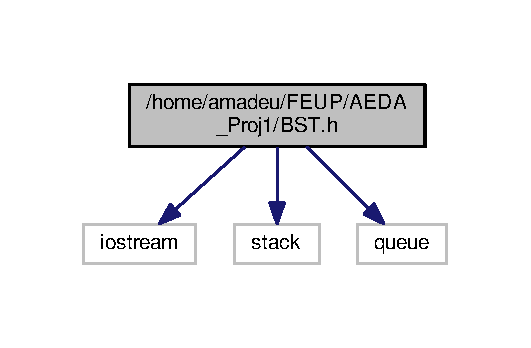
\includegraphics[width=255pt]{BST_8h__incl}
\end{center}
\end{figure}
This graph shows which files directly or indirectly include this file\+:
\nopagebreak
\begin{figure}[H]
\begin{center}
\leavevmode
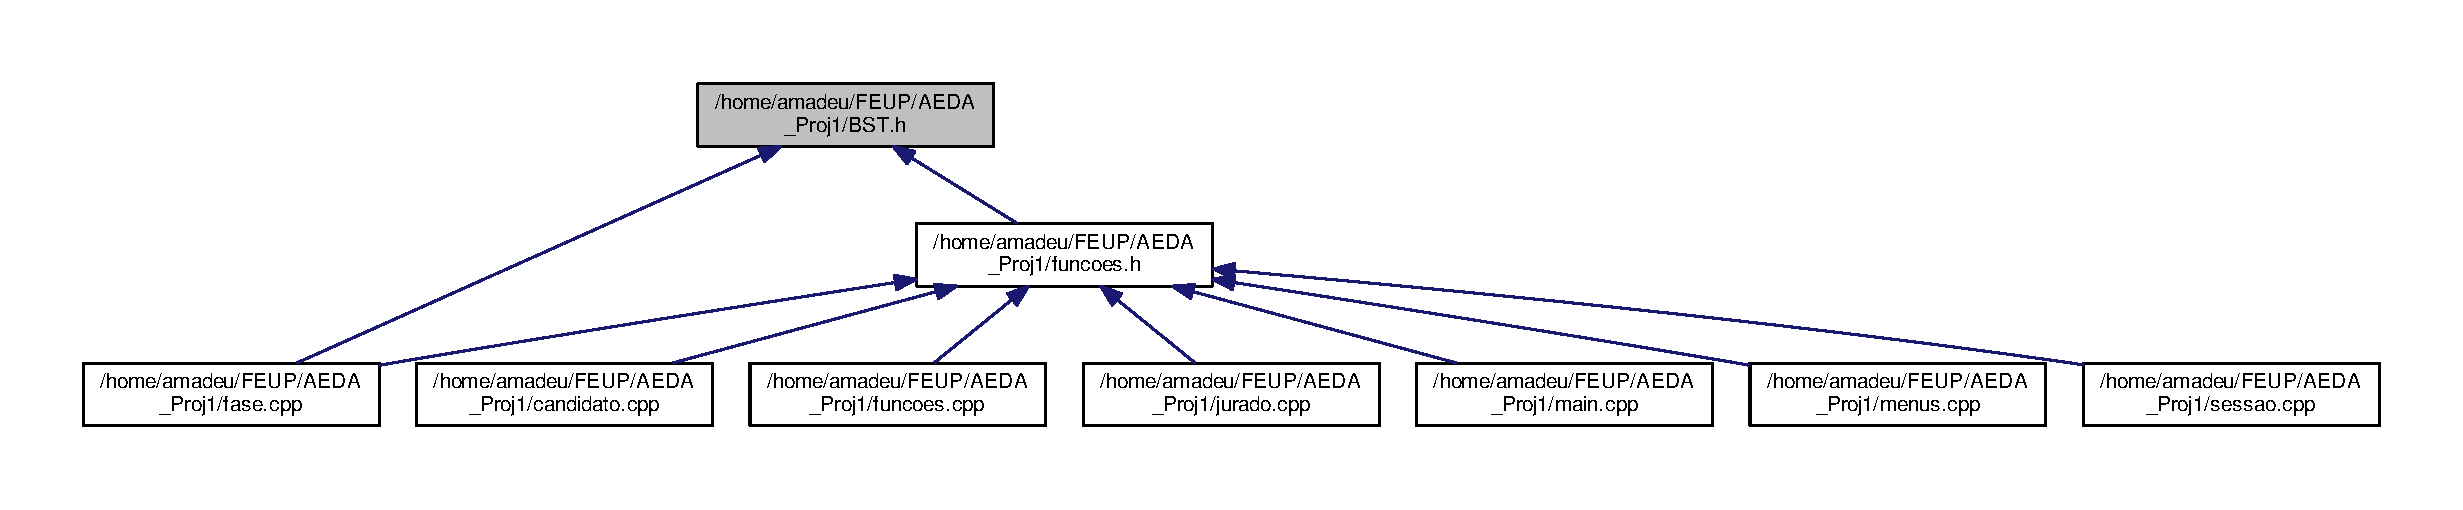
\includegraphics[width=350pt]{BST_8h__dep__incl}
\end{center}
\end{figure}
\subsection*{Classes}
\begin{DoxyCompactItemize}
\item 
class \hyperlink{classBSTItrIn}{B\+S\+T\+Itr\+In$<$ Comparable $>$}
\item 
class \hyperlink{classBSTItrPre}{B\+S\+T\+Itr\+Pre$<$ Comparable $>$}
\item 
class \hyperlink{classBSTItrPost}{B\+S\+T\+Itr\+Post$<$ Comparable $>$}
\item 
class \hyperlink{classBSTItrLevel}{B\+S\+T\+Itr\+Level$<$ Comparable $>$}
\item 
class \hyperlink{classBST}{B\+S\+T$<$ Comparable $>$}
\item 
class \hyperlink{classBinaryNode}{Binary\+Node$<$ Comparable $>$}
\item 
class \hyperlink{classBST}{B\+S\+T$<$ Comparable $>$}
\item 
class \hyperlink{classBSTItrPost}{B\+S\+T\+Itr\+Post$<$ Comparable $>$}
\item 
class \hyperlink{classBSTItrPre}{B\+S\+T\+Itr\+Pre$<$ Comparable $>$}
\item 
class \hyperlink{classBSTItrIn}{B\+S\+T\+Itr\+In$<$ Comparable $>$}
\item 
class \hyperlink{classBSTItrLevel}{B\+S\+T\+Itr\+Level$<$ Comparable $>$}
\end{DoxyCompactItemize}

\hypertarget{candidato_8cpp}{}\section{/home/amadeu/\+F\+E\+U\+P/\+A\+E\+D\+A\+\_\+\+Proj1/candidato.cpp File Reference}
\label{candidato_8cpp}\index{/home/amadeu/\+F\+E\+U\+P/\+A\+E\+D\+A\+\_\+\+Proj1/candidato.\+cpp@{/home/amadeu/\+F\+E\+U\+P/\+A\+E\+D\+A\+\_\+\+Proj1/candidato.\+cpp}}
{\ttfamily \#include \char`\"{}candidato.\+h\char`\"{}}\\*
{\ttfamily \#include \char`\"{}funcoes.\+h\char`\"{}}\\*
Include dependency graph for candidato.\+cpp\+:
\nopagebreak
\begin{figure}[H]
\begin{center}
\leavevmode
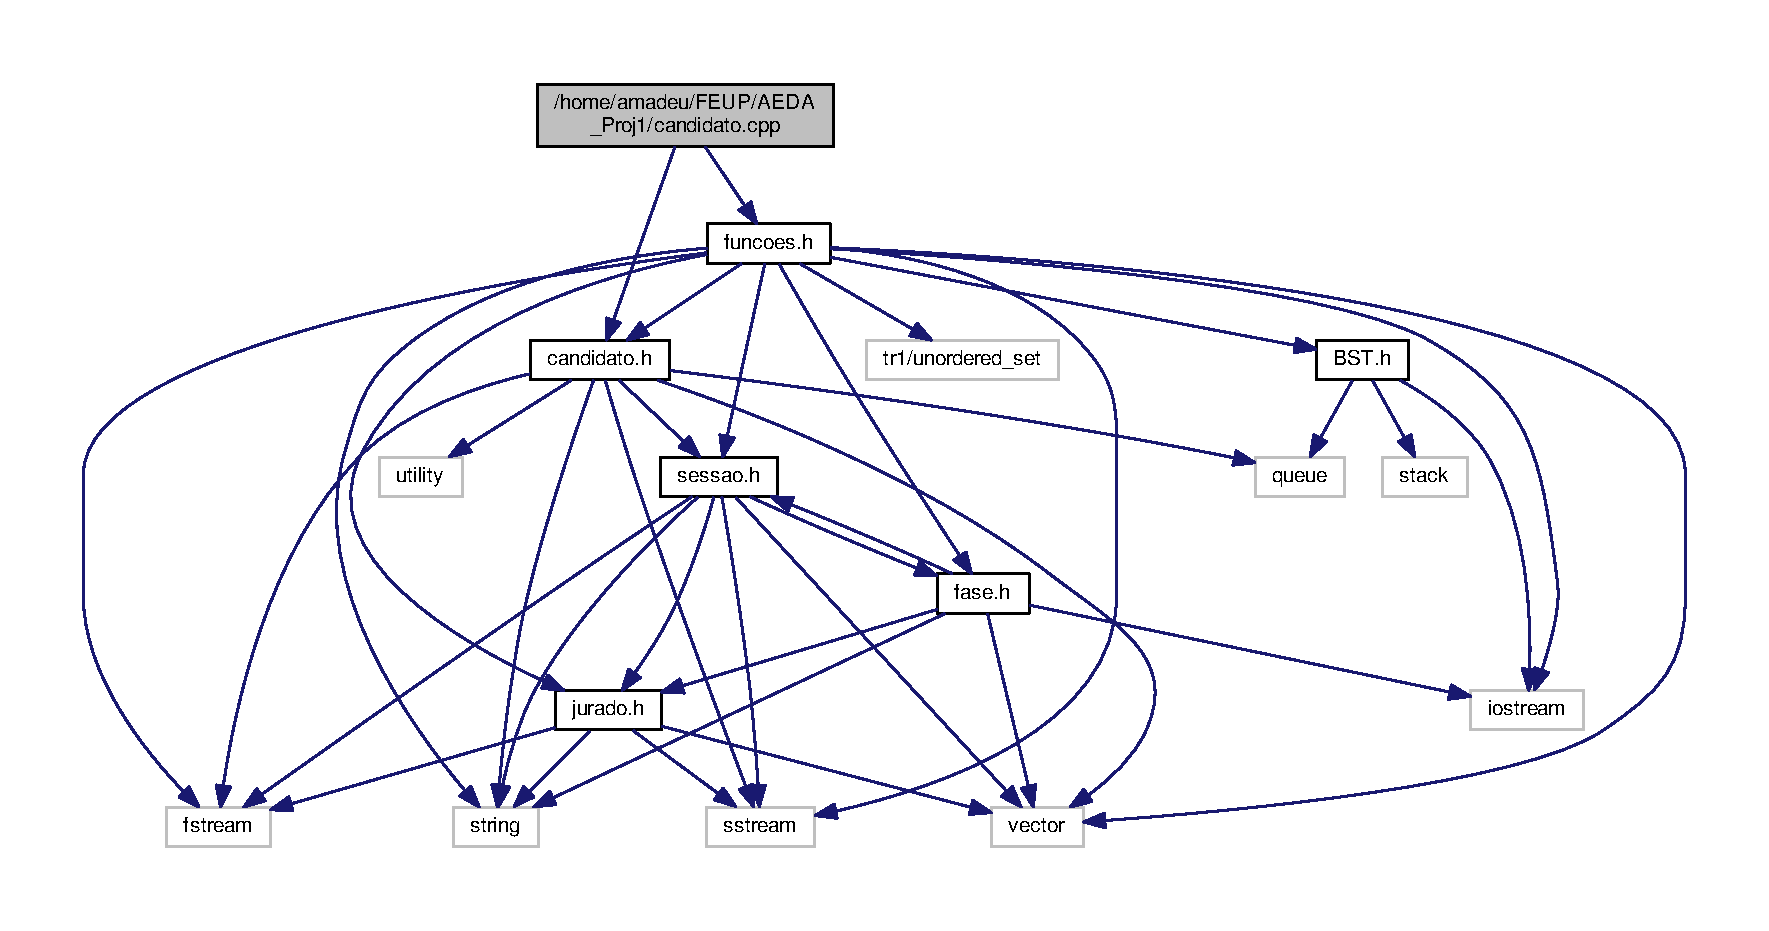
\includegraphics[width=350pt]{candidato_8cpp__incl}
\end{center}
\end{figure}
\subsection*{Functions}
\begin{DoxyCompactItemize}
\item 
std\+::ostream \& \hyperlink{candidato_8cpp_a20e6529edb342e321b8dae17eabbeb7f}{operator$<$$<$} (std\+::ostream \&out, const \hyperlink{classcandidatoJaExiste}{candidato\+Ja\+Existe} \&c)
\begin{DoxyCompactList}\small\item\em overload do operador$<$$<$ para elementos da class \hyperlink{classcandidatoJaExiste}{candidato\+Ja\+Existe} \end{DoxyCompactList}\item 
std\+::ostream \& \hyperlink{candidato_8cpp_a02901504981000fd21efbed6bd16811a}{operator$<$$<$} (std\+::ostream \&out, const \hyperlink{classcandidatoNaoExiste}{candidato\+Nao\+Existe} \&c)
\begin{DoxyCompactList}\small\item\em overload do operador$<$$<$ para elementos da class \hyperlink{classcandidatoNaoExiste}{candidato\+Nao\+Existe} \end{DoxyCompactList}\item 
std\+::ostream \& \hyperlink{candidato_8cpp_a200a248ef11fbf0057a9eb376406e003}{operator$<$$<$} (std\+::ostream \&out, const \hyperlink{classcandidatoOcupado}{candidato\+Ocupado} \&c)
\begin{DoxyCompactList}\small\item\em overload do operador$<$$<$ para elementos da class \hyperlink{classcandidatoOcupado}{candidato\+Ocupado} \end{DoxyCompactList}\item 
ostream \& \hyperlink{candidato_8cpp_a8b349878e0149761fba4bccf3c7d5148}{operator$<$$<$} (ostream \&o, const \hyperlink{classcandidato}{candidato} \&c)
\item 
ofstream \& \hyperlink{candidato_8cpp_ad86b8f19b641b7c48c5c695a8f15f9a2}{operator$<$$<$} (ofstream \&o, const \hyperlink{classcandidato}{candidato} \&c)
\end{DoxyCompactItemize}


\subsection{Function Documentation}
\index{candidato.\+cpp@{candidato.\+cpp}!operator$<$$<$@{operator$<$$<$}}
\index{operator$<$$<$@{operator$<$$<$}!candidato.\+cpp@{candidato.\+cpp}}
\subsubsection[{\texorpdfstring{operator$<$$<$(std\+::ostream \&out, const candidato\+Ja\+Existe \&c)}{operator<<(std::ostream &out, const candidatoJaExiste &c)}}]{\setlength{\rightskip}{0pt plus 5cm}std\+::ostream\& operator$<$$<$ (
\begin{DoxyParamCaption}
\item[{std\+::ostream \&}]{out, }
\item[{const {\bf candidato\+Ja\+Existe} \&}]{c}
\end{DoxyParamCaption}
)}\hypertarget{candidato_8cpp_a20e6529edb342e321b8dae17eabbeb7f}{}\label{candidato_8cpp_a20e6529edb342e321b8dae17eabbeb7f}


overload do operador$<$$<$ para elementos da class \hyperlink{classcandidatoJaExiste}{candidato\+Ja\+Existe} 

\index{candidato.\+cpp@{candidato.\+cpp}!operator$<$$<$@{operator$<$$<$}}
\index{operator$<$$<$@{operator$<$$<$}!candidato.\+cpp@{candidato.\+cpp}}
\subsubsection[{\texorpdfstring{operator$<$$<$(std\+::ostream \&out, const candidato\+Nao\+Existe \&c)}{operator<<(std::ostream &out, const candidatoNaoExiste &c)}}]{\setlength{\rightskip}{0pt plus 5cm}std\+::ostream\& operator$<$$<$ (
\begin{DoxyParamCaption}
\item[{std\+::ostream \&}]{out, }
\item[{const {\bf candidato\+Nao\+Existe} \&}]{c}
\end{DoxyParamCaption}
)}\hypertarget{candidato_8cpp_a02901504981000fd21efbed6bd16811a}{}\label{candidato_8cpp_a02901504981000fd21efbed6bd16811a}


overload do operador$<$$<$ para elementos da class \hyperlink{classcandidatoNaoExiste}{candidato\+Nao\+Existe} 

\index{candidato.\+cpp@{candidato.\+cpp}!operator$<$$<$@{operator$<$$<$}}
\index{operator$<$$<$@{operator$<$$<$}!candidato.\+cpp@{candidato.\+cpp}}
\subsubsection[{\texorpdfstring{operator$<$$<$(std\+::ostream \&out, const candidato\+Ocupado \&c)}{operator<<(std::ostream &out, const candidatoOcupado &c)}}]{\setlength{\rightskip}{0pt plus 5cm}std\+::ostream\& operator$<$$<$ (
\begin{DoxyParamCaption}
\item[{std\+::ostream \&}]{out, }
\item[{const {\bf candidato\+Ocupado} \&}]{c}
\end{DoxyParamCaption}
)}\hypertarget{candidato_8cpp_a200a248ef11fbf0057a9eb376406e003}{}\label{candidato_8cpp_a200a248ef11fbf0057a9eb376406e003}


overload do operador$<$$<$ para elementos da class \hyperlink{classcandidatoOcupado}{candidato\+Ocupado} 

\index{candidato.\+cpp@{candidato.\+cpp}!operator$<$$<$@{operator$<$$<$}}
\index{operator$<$$<$@{operator$<$$<$}!candidato.\+cpp@{candidato.\+cpp}}
\subsubsection[{\texorpdfstring{operator$<$$<$(ostream \&o, const candidato \&c)}{operator<<(ostream &o, const candidato &c)}}]{\setlength{\rightskip}{0pt plus 5cm}ostream\& operator$<$$<$ (
\begin{DoxyParamCaption}
\item[{ostream \&}]{o, }
\item[{const {\bf candidato} \&}]{c}
\end{DoxyParamCaption}
)}\hypertarget{candidato_8cpp_a8b349878e0149761fba4bccf3c7d5148}{}\label{candidato_8cpp_a8b349878e0149761fba4bccf3c7d5148}
\index{candidato.\+cpp@{candidato.\+cpp}!operator$<$$<$@{operator$<$$<$}}
\index{operator$<$$<$@{operator$<$$<$}!candidato.\+cpp@{candidato.\+cpp}}
\subsubsection[{\texorpdfstring{operator$<$$<$(ofstream \&o, const candidato \&c)}{operator<<(ofstream &o, const candidato &c)}}]{\setlength{\rightskip}{0pt plus 5cm}ofstream\& operator$<$$<$ (
\begin{DoxyParamCaption}
\item[{ofstream \&}]{o, }
\item[{const {\bf candidato} \&}]{c}
\end{DoxyParamCaption}
)}\hypertarget{candidato_8cpp_ad86b8f19b641b7c48c5c695a8f15f9a2}{}\label{candidato_8cpp_ad86b8f19b641b7c48c5c695a8f15f9a2}

\hypertarget{candidato_8h}{}\section{/home/amadeu/\+F\+E\+U\+P/\+A\+E\+D\+A\+\_\+\+Proj1/candidato.h File Reference}
\label{candidato_8h}\index{/home/amadeu/\+F\+E\+U\+P/\+A\+E\+D\+A\+\_\+\+Proj1/candidato.\+h@{/home/amadeu/\+F\+E\+U\+P/\+A\+E\+D\+A\+\_\+\+Proj1/candidato.\+h}}
{\ttfamily \#include $<$string$>$}\\*
{\ttfamily \#include $<$vector$>$}\\*
{\ttfamily \#include $<$sstream$>$}\\*
{\ttfamily \#include $<$fstream$>$}\\*
{\ttfamily \#include $<$utility$>$}\\*
{\ttfamily \#include $<$queue$>$}\\*
{\ttfamily \#include \char`\"{}sessao.\+h\char`\"{}}\\*
Include dependency graph for candidato.\+h\+:
\nopagebreak
\begin{figure}[H]
\begin{center}
\leavevmode
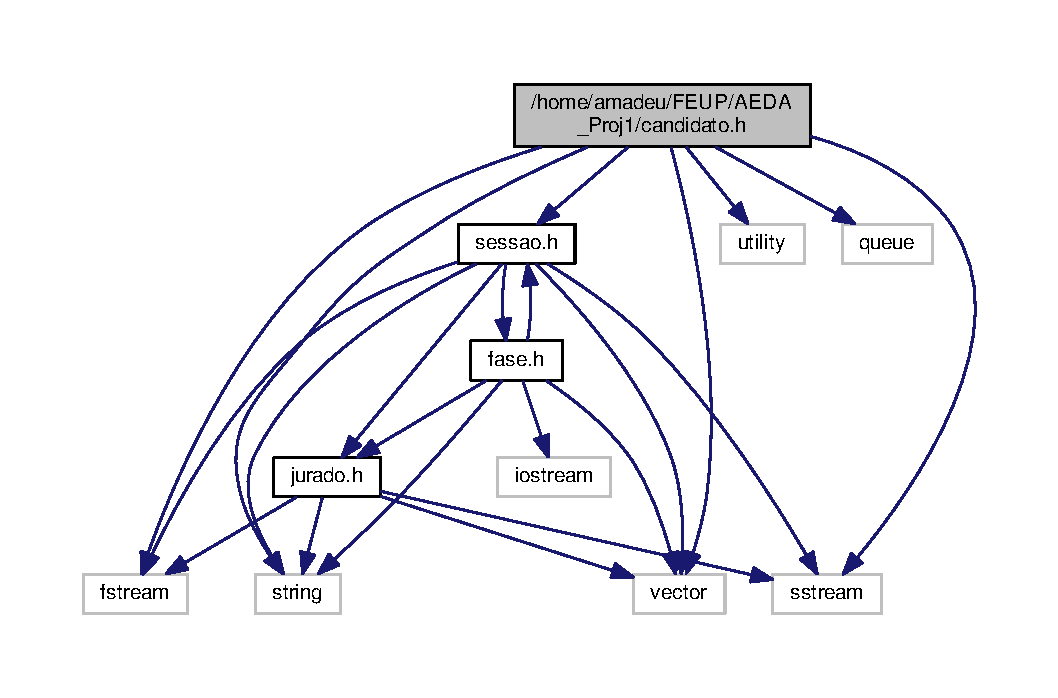
\includegraphics[width=350pt]{candidato_8h__incl}
\end{center}
\end{figure}
This graph shows which files directly or indirectly include this file\+:
\nopagebreak
\begin{figure}[H]
\begin{center}
\leavevmode
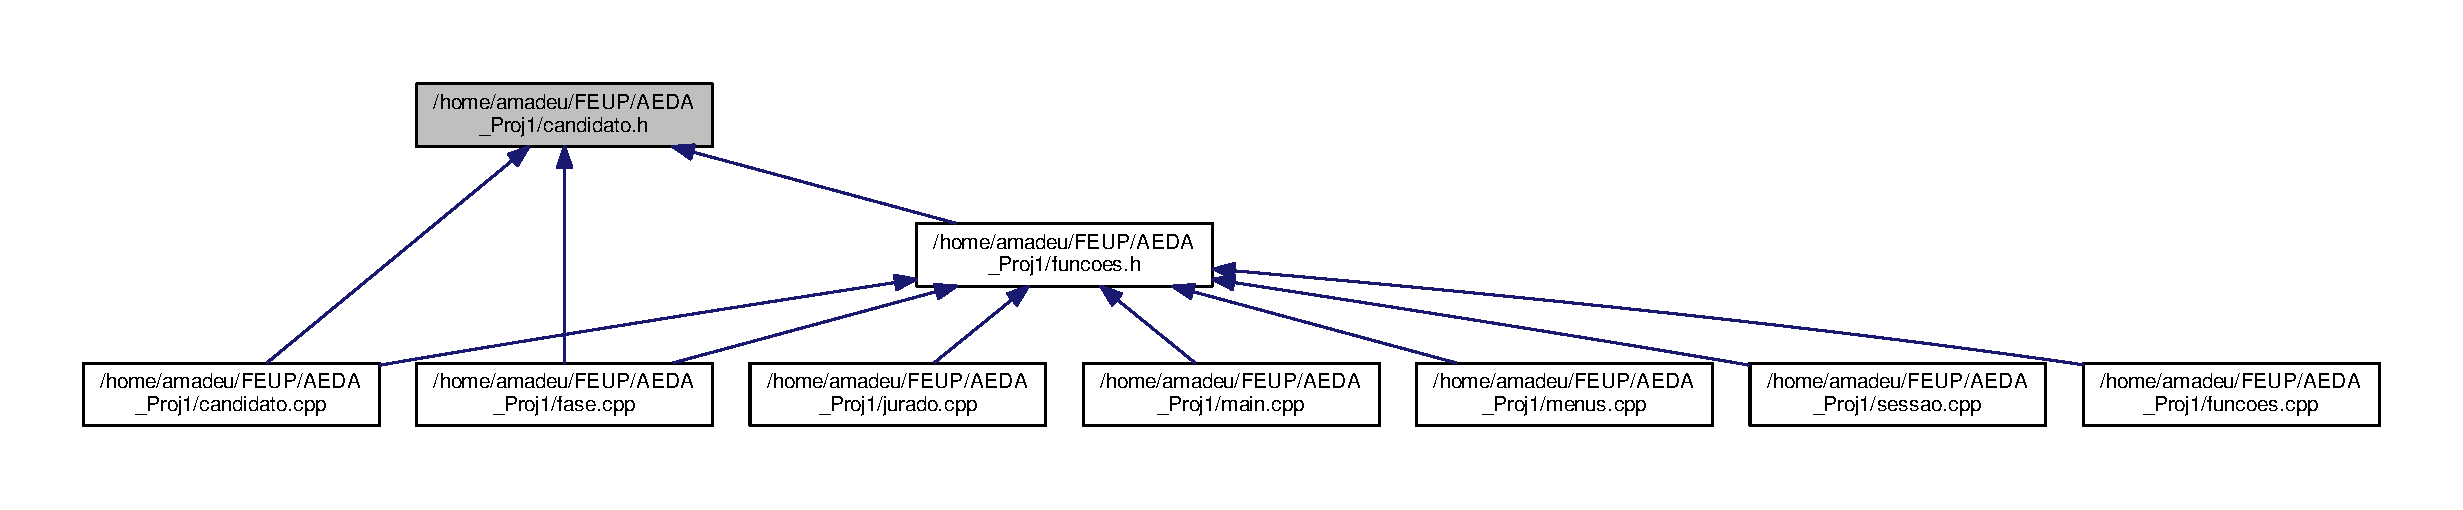
\includegraphics[width=350pt]{candidato_8h__dep__incl}
\end{center}
\end{figure}
\subsection*{Classes}
\begin{DoxyCompactItemize}
\item 
class \hyperlink{classcandidato}{candidato}
\begin{DoxyCompactList}\small\item\em classe com as informacoes relativas a um candidato \end{DoxyCompactList}\item 
class \hyperlink{classcandidatoNaoExiste}{candidato\+Nao\+Existe}
\begin{DoxyCompactList}\small\item\em excepcao para quando um objeto da classe candidato nao existe \end{DoxyCompactList}\item 
class \hyperlink{classcandidatoJaExiste}{candidato\+Ja\+Existe}
\begin{DoxyCompactList}\small\item\em excepcao para quando um objeto da classe candidato ja existe \end{DoxyCompactList}\item 
class \hyperlink{classcandidatoOcupado}{candidato\+Ocupado}
\begin{DoxyCompactList}\small\item\em excepcao para quando um objeto da classe candidato ja ja se encontra ocupado num determinado dia \end{DoxyCompactList}\end{DoxyCompactItemize}
\subsection*{Functions}
\begin{DoxyCompactItemize}
\item 
std\+::ostream \& \hyperlink{candidato_8h_a02901504981000fd21efbed6bd16811a}{operator$<$$<$} (std\+::ostream \&out, const \hyperlink{classcandidatoNaoExiste}{candidato\+Nao\+Existe} \&c)
\begin{DoxyCompactList}\small\item\em overload do operador$<$$<$ para elementos da class \hyperlink{classcandidatoNaoExiste}{candidato\+Nao\+Existe} \end{DoxyCompactList}\item 
std\+::ostream \& \hyperlink{candidato_8h_a20e6529edb342e321b8dae17eabbeb7f}{operator$<$$<$} (std\+::ostream \&out, const \hyperlink{classcandidatoJaExiste}{candidato\+Ja\+Existe} \&c)
\begin{DoxyCompactList}\small\item\em overload do operador$<$$<$ para elementos da class \hyperlink{classcandidatoJaExiste}{candidato\+Ja\+Existe} \end{DoxyCompactList}\item 
std\+::ostream \& \hyperlink{candidato_8h_a200a248ef11fbf0057a9eb376406e003}{operator$<$$<$} (std\+::ostream \&out, const \hyperlink{classcandidatoOcupado}{candidato\+Ocupado} \&c)
\begin{DoxyCompactList}\small\item\em overload do operador$<$$<$ para elementos da class \hyperlink{classcandidatoOcupado}{candidato\+Ocupado} \end{DoxyCompactList}\end{DoxyCompactItemize}


\subsection{Function Documentation}
\index{candidato.\+h@{candidato.\+h}!operator$<$$<$@{operator$<$$<$}}
\index{operator$<$$<$@{operator$<$$<$}!candidato.\+h@{candidato.\+h}}
\subsubsection[{\texorpdfstring{operator$<$$<$(std\+::ostream \&out, const candidato\+Nao\+Existe \&c)}{operator<<(std::ostream &out, const candidatoNaoExiste &c)}}]{\setlength{\rightskip}{0pt plus 5cm}std\+::ostream\& operator$<$$<$ (
\begin{DoxyParamCaption}
\item[{std\+::ostream \&}]{out, }
\item[{const {\bf candidato\+Nao\+Existe} \&}]{c}
\end{DoxyParamCaption}
)}\hypertarget{candidato_8h_a02901504981000fd21efbed6bd16811a}{}\label{candidato_8h_a02901504981000fd21efbed6bd16811a}


overload do operador$<$$<$ para elementos da class \hyperlink{classcandidatoNaoExiste}{candidato\+Nao\+Existe} 

\index{candidato.\+h@{candidato.\+h}!operator$<$$<$@{operator$<$$<$}}
\index{operator$<$$<$@{operator$<$$<$}!candidato.\+h@{candidato.\+h}}
\subsubsection[{\texorpdfstring{operator$<$$<$(std\+::ostream \&out, const candidato\+Ja\+Existe \&c)}{operator<<(std::ostream &out, const candidatoJaExiste &c)}}]{\setlength{\rightskip}{0pt plus 5cm}std\+::ostream\& operator$<$$<$ (
\begin{DoxyParamCaption}
\item[{std\+::ostream \&}]{out, }
\item[{const {\bf candidato\+Ja\+Existe} \&}]{c}
\end{DoxyParamCaption}
)}\hypertarget{candidato_8h_a20e6529edb342e321b8dae17eabbeb7f}{}\label{candidato_8h_a20e6529edb342e321b8dae17eabbeb7f}


overload do operador$<$$<$ para elementos da class \hyperlink{classcandidatoJaExiste}{candidato\+Ja\+Existe} 

\index{candidato.\+h@{candidato.\+h}!operator$<$$<$@{operator$<$$<$}}
\index{operator$<$$<$@{operator$<$$<$}!candidato.\+h@{candidato.\+h}}
\subsubsection[{\texorpdfstring{operator$<$$<$(std\+::ostream \&out, const candidato\+Ocupado \&c)}{operator<<(std::ostream &out, const candidatoOcupado &c)}}]{\setlength{\rightskip}{0pt plus 5cm}std\+::ostream\& operator$<$$<$ (
\begin{DoxyParamCaption}
\item[{std\+::ostream \&}]{out, }
\item[{const {\bf candidato\+Ocupado} \&}]{c}
\end{DoxyParamCaption}
)}\hypertarget{candidato_8h_a200a248ef11fbf0057a9eb376406e003}{}\label{candidato_8h_a200a248ef11fbf0057a9eb376406e003}


overload do operador$<$$<$ para elementos da class \hyperlink{classcandidatoOcupado}{candidato\+Ocupado} 


\hypertarget{candidatos_8txt}{}\section{/home/amadeu/\+F\+E\+U\+P/\+A\+E\+D\+A\+\_\+\+Proj1/candidatos.txt File Reference}
\label{candidatos_8txt}\index{/home/amadeu/\+F\+E\+U\+P/\+A\+E\+D\+A\+\_\+\+Proj1/candidatos.\+txt@{/home/amadeu/\+F\+E\+U\+P/\+A\+E\+D\+A\+\_\+\+Proj1/candidatos.\+txt}}
\subsection*{Variables}
\begin{DoxyCompactItemize}
\item 
\hyperlink{candidatos_8txt_a6414eb73c2395148093f8baa9e202616}{Joao}
\item 
vila \hyperlink{candidatos_8txt_a38df1df7696364439f75acd6d9e12db3}{real}
\item 
vila \hyperlink{candidatos_8txt_ad6218b62b1662d9aecef7e5202e38585}{cantar}
\item 
vila \hyperlink{candidatos_8txt_aab193da33fe7af81c3f38956a69ddc7b}{Afonso}
\item 
vila \hyperlink{candidatos_8txt_a50f37943ca5db274938bcee517a283cc}{porto}
\item 
vila \hyperlink{candidatos_8txt_a46623e301f4e03cb83c7fbeb8b1a7f43}{aulas}
\item 
\hyperlink{candidatos_8txt_afae26757e6180cef120017b01ac06140}{Rui}
\item 
\hyperlink{candidatos_8txt_ae97c2e40b26f85d0c45fbaf917d77502}{Roberto}
\item 
\hyperlink{candidatos_8txt_a1bb862406aa43586e05f956f8e9cabb1}{chaves}
\item 
\hyperlink{candidatos_8txt_ad6339a08af3e0ee859de202f9944116b}{trabalho}
\item 
\hyperlink{candidatos_8txt_aaa4a8e584997e199066f8f4910bf4ead}{Andreia}
\item 
\hyperlink{candidatos_8txt_a33e5ff5ddbb7118468c3dd458466532b}{Bruno}
\item 
\hyperlink{candidatos_8txt_afcb0be523bb30dc71d43c136869e3683}{lisboa}
\item 
\hyperlink{candidatos_8txt_a508a855615268f4003a2dcef768b5abe}{Ricardo}
\item 
\hyperlink{candidatos_8txt_a8c64f18bebe8b957cbc75ce757dd3af4}{Carlos}
\item 
\hyperlink{candidatos_8txt_ab0e2bf38e63ce27dd973bc5f810a5342}{algarve}
\item 
\hyperlink{candidatos_8txt_a0fa004e8ae93e7afad527aaa2bb04dff}{Raquel}
\item 
viana do \hyperlink{candidatos_8txt_a7a3d2fede813d5b19ee63499917664e2}{castelo}
\item 
viana do \hyperlink{candidatos_8txt_a7a54d64ce86da7c9cb1cec1f9b572e14}{dancar}
\item 
viana do \hyperlink{sessoes_8txt_a0375353ca858a7b935ff53ef0a3c9a98}{Maria} \hyperlink{candidatos_8txt_adc6ee4336af7550893efe711a3ee0570}{faro}
\item 
viana do \hyperlink{sessoes_8txt_a0375353ca858a7b935ff53ef0a3c9a98}{Maria} \hyperlink{candidatos_8txt_a9d93dce88080548099a56cf093e4bba9}{Helena}
\item 
viana do \hyperlink{sessoes_8txt_a0375353ca858a7b935ff53ef0a3c9a98}{Maria} \hyperlink{candidatos_8txt_ad48e47e2e0f1add17c5dcd5c9dfc1381}{Antonio}
\item 
viana do \hyperlink{sessoes_8txt_a0375353ca858a7b935ff53ef0a3c9a98}{Maria} \hyperlink{candidatos_8txt_acb9307bae8c337dfbd877babfe36f1ad}{braga}
\item 
viana do \hyperlink{sessoes_8txt_a0375353ca858a7b935ff53ef0a3c9a98}{Maria} \hyperlink{candidatos_8txt_a9439c806cb17f3371bbee523ca9b13ec}{Marta}
\item 
viana do \hyperlink{sessoes_8txt_a0375353ca858a7b935ff53ef0a3c9a98}{Maria} \hyperlink{candidatos_8txt_a59134b75acc1ed74b176c98faefd5e9b}{magia}
\item 
viana do \hyperlink{sessoes_8txt_a0375353ca858a7b935ff53ef0a3c9a98}{Maria} \hyperlink{candidatos_8txt_af84719fafa1b55d65980e3a27b236714}{Pedro}
\item 
viana do \hyperlink{sessoes_8txt_a0375353ca858a7b935ff53ef0a3c9a98}{Maria} \hyperlink{candidatos_8txt_ae645720a55439c3bfd303f6840c137b1}{Josefa}
\end{DoxyCompactItemize}


\subsection{Variable Documentation}
\index{candidatos.\+txt@{candidatos.\+txt}!Afonso@{Afonso}}
\index{Afonso@{Afonso}!candidatos.\+txt@{candidatos.\+txt}}
\subsubsection[{\texorpdfstring{Afonso}{Afonso}}]{\setlength{\rightskip}{0pt plus 5cm}vila Afonso}\hypertarget{candidatos_8txt_aab193da33fe7af81c3f38956a69ddc7b}{}\label{candidatos_8txt_aab193da33fe7af81c3f38956a69ddc7b}
\index{candidatos.\+txt@{candidatos.\+txt}!algarve@{algarve}}
\index{algarve@{algarve}!candidatos.\+txt@{candidatos.\+txt}}
\subsubsection[{\texorpdfstring{algarve}{algarve}}]{\setlength{\rightskip}{0pt plus 5cm}algarve}\hypertarget{candidatos_8txt_ab0e2bf38e63ce27dd973bc5f810a5342}{}\label{candidatos_8txt_ab0e2bf38e63ce27dd973bc5f810a5342}
\index{candidatos.\+txt@{candidatos.\+txt}!Andreia@{Andreia}}
\index{Andreia@{Andreia}!candidatos.\+txt@{candidatos.\+txt}}
\subsubsection[{\texorpdfstring{Andreia}{Andreia}}]{\setlength{\rightskip}{0pt plus 5cm}Andreia}\hypertarget{candidatos_8txt_aaa4a8e584997e199066f8f4910bf4ead}{}\label{candidatos_8txt_aaa4a8e584997e199066f8f4910bf4ead}
\index{candidatos.\+txt@{candidatos.\+txt}!Antonio@{Antonio}}
\index{Antonio@{Antonio}!candidatos.\+txt@{candidatos.\+txt}}
\subsubsection[{\texorpdfstring{Antonio}{Antonio}}]{\setlength{\rightskip}{0pt plus 5cm}{\bf Maria} {\bf Maria} Antonio}\hypertarget{candidatos_8txt_ad48e47e2e0f1add17c5dcd5c9dfc1381}{}\label{candidatos_8txt_ad48e47e2e0f1add17c5dcd5c9dfc1381}
\index{candidatos.\+txt@{candidatos.\+txt}!aulas@{aulas}}
\index{aulas@{aulas}!candidatos.\+txt@{candidatos.\+txt}}
\subsubsection[{\texorpdfstring{aulas}{aulas}}]{\setlength{\rightskip}{0pt plus 5cm}aulas}\hypertarget{candidatos_8txt_a46623e301f4e03cb83c7fbeb8b1a7f43}{}\label{candidatos_8txt_a46623e301f4e03cb83c7fbeb8b1a7f43}
\index{candidatos.\+txt@{candidatos.\+txt}!braga@{braga}}
\index{braga@{braga}!candidatos.\+txt@{candidatos.\+txt}}
\subsubsection[{\texorpdfstring{braga}{braga}}]{\setlength{\rightskip}{0pt plus 5cm}{\bf dancar} {\bf dancar} {\bf cantar} braga}\hypertarget{candidatos_8txt_acb9307bae8c337dfbd877babfe36f1ad}{}\label{candidatos_8txt_acb9307bae8c337dfbd877babfe36f1ad}
\index{candidatos.\+txt@{candidatos.\+txt}!Bruno@{Bruno}}
\index{Bruno@{Bruno}!candidatos.\+txt@{candidatos.\+txt}}
\subsubsection[{\texorpdfstring{Bruno}{Bruno}}]{\setlength{\rightskip}{0pt plus 5cm}Bruno}\hypertarget{candidatos_8txt_a33e5ff5ddbb7118468c3dd458466532b}{}\label{candidatos_8txt_a33e5ff5ddbb7118468c3dd458466532b}
\index{candidatos.\+txt@{candidatos.\+txt}!cantar@{cantar}}
\index{cantar@{cantar}!candidatos.\+txt@{candidatos.\+txt}}
\subsubsection[{\texorpdfstring{cantar}{cantar}}]{\setlength{\rightskip}{0pt plus 5cm}vila cantar}\hypertarget{candidatos_8txt_ad6218b62b1662d9aecef7e5202e38585}{}\label{candidatos_8txt_ad6218b62b1662d9aecef7e5202e38585}
\index{candidatos.\+txt@{candidatos.\+txt}!Carlos@{Carlos}}
\index{Carlos@{Carlos}!candidatos.\+txt@{candidatos.\+txt}}
\subsubsection[{\texorpdfstring{Carlos}{Carlos}}]{\setlength{\rightskip}{0pt plus 5cm}Carlos}\hypertarget{candidatos_8txt_a8c64f18bebe8b957cbc75ce757dd3af4}{}\label{candidatos_8txt_a8c64f18bebe8b957cbc75ce757dd3af4}
\index{candidatos.\+txt@{candidatos.\+txt}!castelo@{castelo}}
\index{castelo@{castelo}!candidatos.\+txt@{candidatos.\+txt}}
\subsubsection[{\texorpdfstring{castelo}{castelo}}]{\setlength{\rightskip}{0pt plus 5cm}viana do castelo}\hypertarget{candidatos_8txt_a7a3d2fede813d5b19ee63499917664e2}{}\label{candidatos_8txt_a7a3d2fede813d5b19ee63499917664e2}
\index{candidatos.\+txt@{candidatos.\+txt}!chaves@{chaves}}
\index{chaves@{chaves}!candidatos.\+txt@{candidatos.\+txt}}
\subsubsection[{\texorpdfstring{chaves}{chaves}}]{\setlength{\rightskip}{0pt plus 5cm}viana do {\bf Maria} chaves}\hypertarget{candidatos_8txt_a1bb862406aa43586e05f956f8e9cabb1}{}\label{candidatos_8txt_a1bb862406aa43586e05f956f8e9cabb1}
\index{candidatos.\+txt@{candidatos.\+txt}!dancar@{dancar}}
\index{dancar@{dancar}!candidatos.\+txt@{candidatos.\+txt}}
\subsubsection[{\texorpdfstring{dancar}{dancar}}]{\setlength{\rightskip}{0pt plus 5cm}{\bf Maria} dancar}\hypertarget{candidatos_8txt_a7a54d64ce86da7c9cb1cec1f9b572e14}{}\label{candidatos_8txt_a7a54d64ce86da7c9cb1cec1f9b572e14}
\index{candidatos.\+txt@{candidatos.\+txt}!faro@{faro}}
\index{faro@{faro}!candidatos.\+txt@{candidatos.\+txt}}
\subsubsection[{\texorpdfstring{faro}{faro}}]{\setlength{\rightskip}{0pt plus 5cm}viana do {\bf Maria} faro}\hypertarget{candidatos_8txt_adc6ee4336af7550893efe711a3ee0570}{}\label{candidatos_8txt_adc6ee4336af7550893efe711a3ee0570}
\index{candidatos.\+txt@{candidatos.\+txt}!Helena@{Helena}}
\index{Helena@{Helena}!candidatos.\+txt@{candidatos.\+txt}}
\subsubsection[{\texorpdfstring{Helena}{Helena}}]{\setlength{\rightskip}{0pt plus 5cm}viana do {\bf Maria} Helena}\hypertarget{candidatos_8txt_a9d93dce88080548099a56cf093e4bba9}{}\label{candidatos_8txt_a9d93dce88080548099a56cf093e4bba9}
\index{candidatos.\+txt@{candidatos.\+txt}!Joao@{Joao}}
\index{Joao@{Joao}!candidatos.\+txt@{candidatos.\+txt}}
\subsubsection[{\texorpdfstring{Joao}{Joao}}]{\setlength{\rightskip}{0pt plus 5cm}{\bf Maria} Joao}\hypertarget{candidatos_8txt_a6414eb73c2395148093f8baa9e202616}{}\label{candidatos_8txt_a6414eb73c2395148093f8baa9e202616}
\index{candidatos.\+txt@{candidatos.\+txt}!Josefa@{Josefa}}
\index{Josefa@{Josefa}!candidatos.\+txt@{candidatos.\+txt}}
\subsubsection[{\texorpdfstring{Josefa}{Josefa}}]{\setlength{\rightskip}{0pt plus 5cm}viana do {\bf Maria} Josefa}\hypertarget{candidatos_8txt_ae645720a55439c3bfd303f6840c137b1}{}\label{candidatos_8txt_ae645720a55439c3bfd303f6840c137b1}
\index{candidatos.\+txt@{candidatos.\+txt}!lisboa@{lisboa}}
\index{lisboa@{lisboa}!candidatos.\+txt@{candidatos.\+txt}}
\subsubsection[{\texorpdfstring{lisboa}{lisboa}}]{\setlength{\rightskip}{0pt plus 5cm}{\bf dancar} {\bf dancar} {\bf cantar} {\bf cantar} {\bf magia} vila {\bf dancar} {\bf dancar} {\bf cantar} {\bf cantar} {\bf magia} lisboa}\hypertarget{candidatos_8txt_afcb0be523bb30dc71d43c136869e3683}{}\label{candidatos_8txt_afcb0be523bb30dc71d43c136869e3683}
\index{candidatos.\+txt@{candidatos.\+txt}!magia@{magia}}
\index{magia@{magia}!candidatos.\+txt@{candidatos.\+txt}}
\subsubsection[{\texorpdfstring{magia}{magia}}]{\setlength{\rightskip}{0pt plus 5cm}viana do {\bf Maria} magia}\hypertarget{candidatos_8txt_a59134b75acc1ed74b176c98faefd5e9b}{}\label{candidatos_8txt_a59134b75acc1ed74b176c98faefd5e9b}
\index{candidatos.\+txt@{candidatos.\+txt}!Marta@{Marta}}
\index{Marta@{Marta}!candidatos.\+txt@{candidatos.\+txt}}
\subsubsection[{\texorpdfstring{Marta}{Marta}}]{\setlength{\rightskip}{0pt plus 5cm}viana do {\bf Maria} Marta}\hypertarget{candidatos_8txt_a9439c806cb17f3371bbee523ca9b13ec}{}\label{candidatos_8txt_a9439c806cb17f3371bbee523ca9b13ec}
\index{candidatos.\+txt@{candidatos.\+txt}!Pedro@{Pedro}}
\index{Pedro@{Pedro}!candidatos.\+txt@{candidatos.\+txt}}
\subsubsection[{\texorpdfstring{Pedro}{Pedro}}]{\setlength{\rightskip}{0pt plus 5cm}viana do {\bf Maria} Pedro}\hypertarget{candidatos_8txt_af84719fafa1b55d65980e3a27b236714}{}\label{candidatos_8txt_af84719fafa1b55d65980e3a27b236714}
\index{candidatos.\+txt@{candidatos.\+txt}!porto@{porto}}
\index{porto@{porto}!candidatos.\+txt@{candidatos.\+txt}}
\subsubsection[{\texorpdfstring{porto}{porto}}]{\setlength{\rightskip}{0pt plus 5cm}{\bf dancar} {\bf dancar} {\bf cantar} {\bf cantar} {\bf magia} vila {\bf dancar} {\bf dancar} {\bf cantar} porto}\hypertarget{candidatos_8txt_a50f37943ca5db274938bcee517a283cc}{}\label{candidatos_8txt_a50f37943ca5db274938bcee517a283cc}
\index{candidatos.\+txt@{candidatos.\+txt}!Raquel@{Raquel}}
\index{Raquel@{Raquel}!candidatos.\+txt@{candidatos.\+txt}}
\subsubsection[{\texorpdfstring{Raquel}{Raquel}}]{\setlength{\rightskip}{0pt plus 5cm}{\bf Maria} {\bf Maria} Raquel}\hypertarget{candidatos_8txt_a0fa004e8ae93e7afad527aaa2bb04dff}{}\label{candidatos_8txt_a0fa004e8ae93e7afad527aaa2bb04dff}
\index{candidatos.\+txt@{candidatos.\+txt}!real@{real}}
\index{real@{real}!candidatos.\+txt@{candidatos.\+txt}}
\subsubsection[{\texorpdfstring{real}{real}}]{\setlength{\rightskip}{0pt plus 5cm}vila real}\hypertarget{candidatos_8txt_a38df1df7696364439f75acd6d9e12db3}{}\label{candidatos_8txt_a38df1df7696364439f75acd6d9e12db3}
\index{candidatos.\+txt@{candidatos.\+txt}!Ricardo@{Ricardo}}
\index{Ricardo@{Ricardo}!candidatos.\+txt@{candidatos.\+txt}}
\subsubsection[{\texorpdfstring{Ricardo}{Ricardo}}]{\setlength{\rightskip}{0pt plus 5cm}Ricardo}\hypertarget{candidatos_8txt_a508a855615268f4003a2dcef768b5abe}{}\label{candidatos_8txt_a508a855615268f4003a2dcef768b5abe}
\index{candidatos.\+txt@{candidatos.\+txt}!Roberto@{Roberto}}
\index{Roberto@{Roberto}!candidatos.\+txt@{candidatos.\+txt}}
\subsubsection[{\texorpdfstring{Roberto}{Roberto}}]{\setlength{\rightskip}{0pt plus 5cm}Roberto}\hypertarget{candidatos_8txt_ae97c2e40b26f85d0c45fbaf917d77502}{}\label{candidatos_8txt_ae97c2e40b26f85d0c45fbaf917d77502}
\index{candidatos.\+txt@{candidatos.\+txt}!Rui@{Rui}}
\index{Rui@{Rui}!candidatos.\+txt@{candidatos.\+txt}}
\subsubsection[{\texorpdfstring{Rui}{Rui}}]{\setlength{\rightskip}{0pt plus 5cm}{\bf dancar} {\bf dancar} {\bf cantar} {\bf cantar} {\bf magia} vila {\bf dancar} {\bf dancar} Rui}\hypertarget{candidatos_8txt_afae26757e6180cef120017b01ac06140}{}\label{candidatos_8txt_afae26757e6180cef120017b01ac06140}
\index{candidatos.\+txt@{candidatos.\+txt}!trabalho@{trabalho}}
\index{trabalho@{trabalho}!candidatos.\+txt@{candidatos.\+txt}}
\subsubsection[{\texorpdfstring{trabalho}{trabalho}}]{\setlength{\rightskip}{0pt plus 5cm}trabalho}\hypertarget{candidatos_8txt_ad6339a08af3e0ee859de202f9944116b}{}\label{candidatos_8txt_ad6339a08af3e0ee859de202f9944116b}

\hypertarget{fase_8cpp}{}\section{/home/amadeu/\+F\+E\+U\+P/\+A\+E\+D\+A\+\_\+\+Proj1/fase.cpp File Reference}
\label{fase_8cpp}\index{/home/amadeu/\+F\+E\+U\+P/\+A\+E\+D\+A\+\_\+\+Proj1/fase.\+cpp@{/home/amadeu/\+F\+E\+U\+P/\+A\+E\+D\+A\+\_\+\+Proj1/fase.\+cpp}}
{\ttfamily \#include \char`\"{}fase.\+h\char`\"{}}\\*
{\ttfamily \#include \char`\"{}candidato.\+h\char`\"{}}\\*
{\ttfamily \#include \char`\"{}B\+S\+T.\+h\char`\"{}}\\*
{\ttfamily \#include \char`\"{}funcoes.\+h\char`\"{}}\\*
Include dependency graph for fase.\+cpp\+:
\nopagebreak
\begin{figure}[H]
\begin{center}
\leavevmode
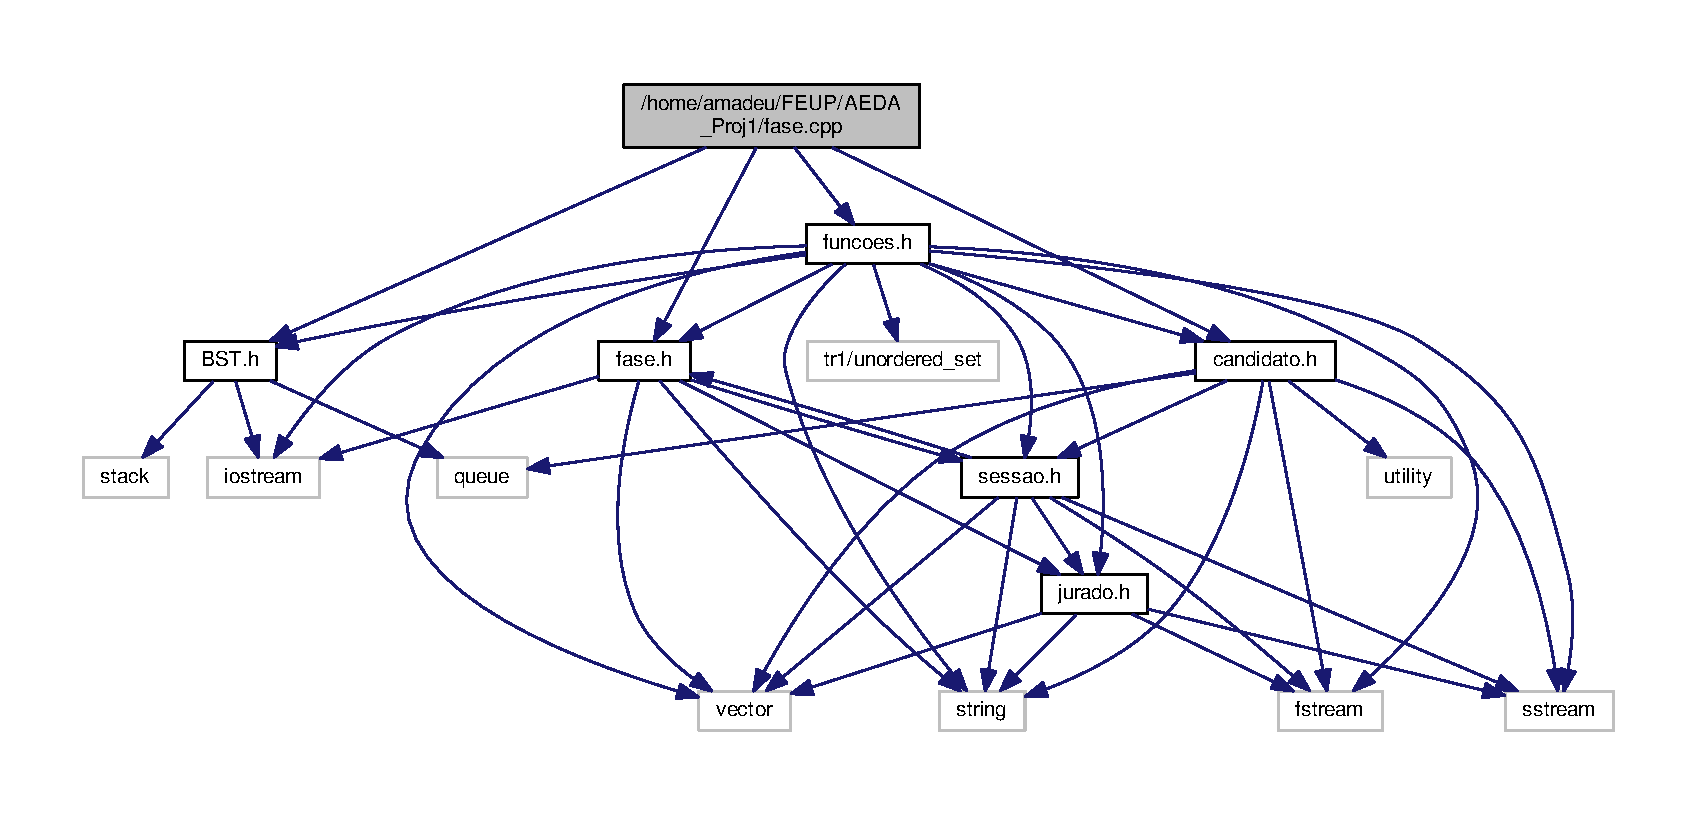
\includegraphics[width=350pt]{fase_8cpp__incl}
\end{center}
\end{figure}
\subsection*{Functions}
\begin{DoxyCompactItemize}
\item 
ostream \& \hyperlink{fase_8cpp_a598506525641a0ba5d116c7d071e80a2}{operator$<$$<$} (ostream \&o, \hyperlink{classfase1}{fase1} f)
\item 
ostream \& \hyperlink{fase_8cpp_a1fcb0da80eaeea4bf75c01e9472bd189}{operator$<$$<$} (ostream \&o, \hyperlink{classfase2}{fase2} f)
\end{DoxyCompactItemize}


\subsection{Function Documentation}
\index{fase.\+cpp@{fase.\+cpp}!operator$<$$<$@{operator$<$$<$}}
\index{operator$<$$<$@{operator$<$$<$}!fase.\+cpp@{fase.\+cpp}}
\subsubsection[{\texorpdfstring{operator$<$$<$(ostream \&o, fase1 f)}{operator<<(ostream &o, fase1 f)}}]{\setlength{\rightskip}{0pt plus 5cm}ostream\& operator$<$$<$ (
\begin{DoxyParamCaption}
\item[{ostream \&}]{o, }
\item[{{\bf fase1}}]{f}
\end{DoxyParamCaption}
)}\hypertarget{fase_8cpp_a598506525641a0ba5d116c7d071e80a2}{}\label{fase_8cpp_a598506525641a0ba5d116c7d071e80a2}
\index{fase.\+cpp@{fase.\+cpp}!operator$<$$<$@{operator$<$$<$}}
\index{operator$<$$<$@{operator$<$$<$}!fase.\+cpp@{fase.\+cpp}}
\subsubsection[{\texorpdfstring{operator$<$$<$(ostream \&o, fase2 f)}{operator<<(ostream &o, fase2 f)}}]{\setlength{\rightskip}{0pt plus 5cm}ostream\& operator$<$$<$ (
\begin{DoxyParamCaption}
\item[{ostream \&}]{o, }
\item[{{\bf fase2}}]{f}
\end{DoxyParamCaption}
)}\hypertarget{fase_8cpp_a1fcb0da80eaeea4bf75c01e9472bd189}{}\label{fase_8cpp_a1fcb0da80eaeea4bf75c01e9472bd189}

\hypertarget{fase_8h}{}\section{/home/amadeu/\+F\+E\+U\+P/\+A\+E\+D\+A\+\_\+\+Proj1/fase.h File Reference}
\label{fase_8h}\index{/home/amadeu/\+F\+E\+U\+P/\+A\+E\+D\+A\+\_\+\+Proj1/fase.\+h@{/home/amadeu/\+F\+E\+U\+P/\+A\+E\+D\+A\+\_\+\+Proj1/fase.\+h}}
{\ttfamily \#include $<$iostream$>$}\\*
{\ttfamily \#include $<$string$>$}\\*
{\ttfamily \#include $<$vector$>$}\\*
{\ttfamily \#include \char`\"{}jurado.\+h\char`\"{}}\\*
{\ttfamily \#include \char`\"{}sessao.\+h\char`\"{}}\\*
Include dependency graph for fase.\+h\+:
\nopagebreak
\begin{figure}[H]
\begin{center}
\leavevmode
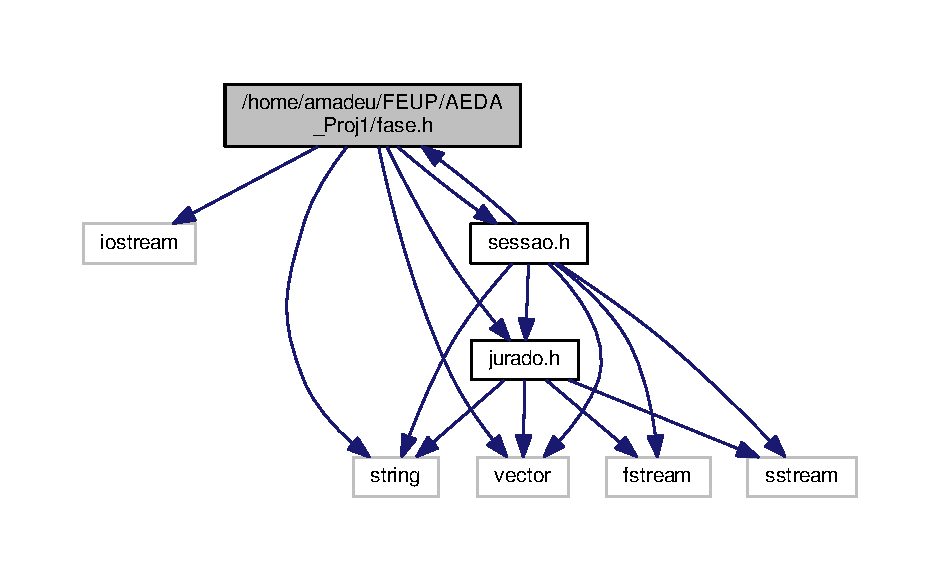
\includegraphics[width=350pt]{fase_8h__incl}
\end{center}
\end{figure}
This graph shows which files directly or indirectly include this file\+:
\nopagebreak
\begin{figure}[H]
\begin{center}
\leavevmode
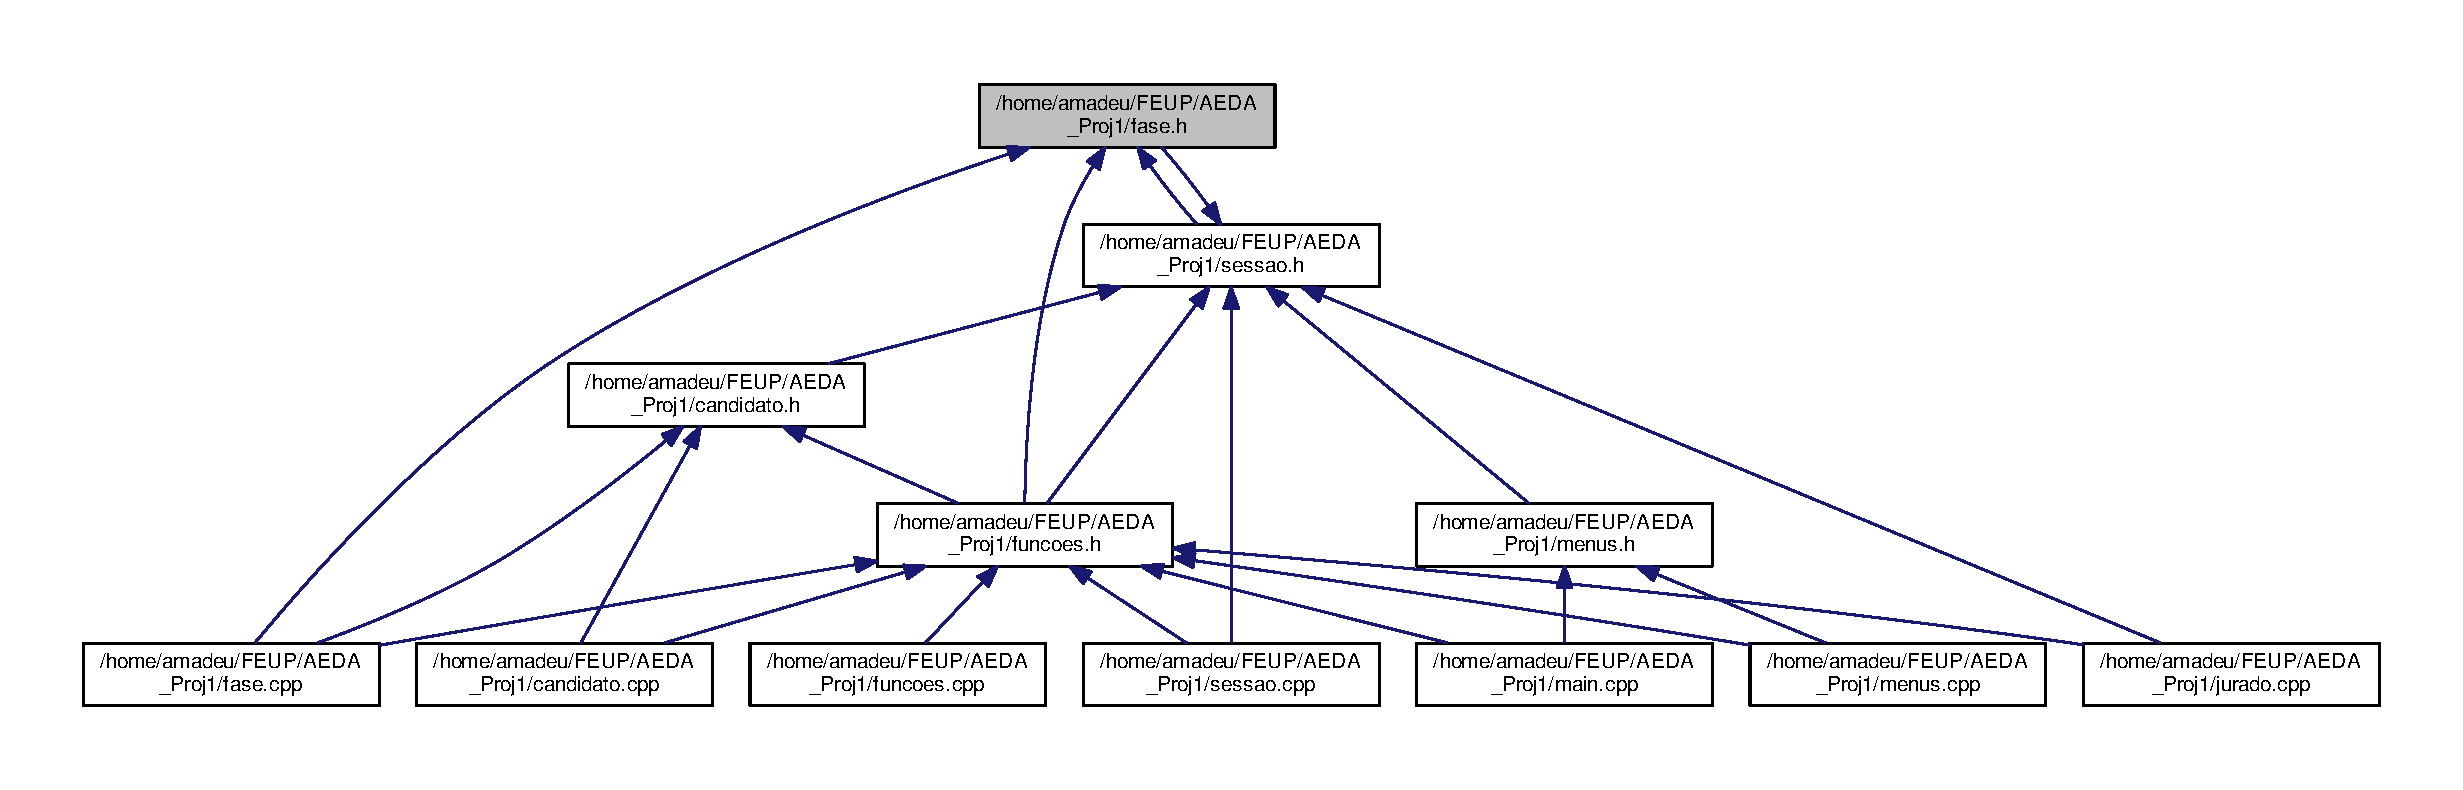
\includegraphics[width=350pt]{fase_8h__dep__incl}
\end{center}
\end{figure}
\subsection*{Classes}
\begin{DoxyCompactItemize}
\item 
struct \hyperlink{structClassificacao}{Classificacao}
\begin{DoxyCompactList}\small\item\em contem a informacao das classificacoes obtidas por um candidato \end{DoxyCompactList}\item 
class \hyperlink{classfase}{fase}
\begin{DoxyCompactList}\small\item\em classe abstrata relativa as varia fases de uma sessao \end{DoxyCompactList}\item 
class \hyperlink{classfase1}{fase1}
\begin{DoxyCompactList}\small\item\em subclasse da classe fase relativa a primeira fase \end{DoxyCompactList}\item 
class \hyperlink{classfase2}{fase2}
\begin{DoxyCompactList}\small\item\em subclasse da classe fase relativa a segunda fase \end{DoxyCompactList}\end{DoxyCompactItemize}

\hypertarget{fases_8txt}{}\section{/home/amadeu/\+F\+E\+U\+P/\+A\+E\+D\+A\+\_\+\+Proj1/fases.txt File Reference}
\label{fases_8txt}\index{/home/amadeu/\+F\+E\+U\+P/\+A\+E\+D\+A\+\_\+\+Proj1/fases.\+txt@{/home/amadeu/\+F\+E\+U\+P/\+A\+E\+D\+A\+\_\+\+Proj1/fases.\+txt}}
\subsection*{Variables}
\begin{DoxyCompactItemize}
\item 
\hyperlink{fases_8txt_a2616159a76d0e8a5493734758ae9c160}{cantar}
\item 
\hyperlink{fases_8txt_a8c64f18bebe8b957cbc75ce757dd3af4}{Carlos}
\item 
\hyperlink{fases_8txt_ae102a7586632535be9ea3d3f64768ab4}{Rui}
\item 
\hyperlink{fases_8txt_a83ec618410e4714b08aa56507a10f025}{Pedro}
\item 
\hyperlink{fases_8txt_a07ad80fe6680f2ac3523954e065ee97d}{Joao}
\item 
\hyperlink{fases_8txt_abc15862bdb1800c6fcdf948e0de62523}{Helena}
\item 
\hyperlink{fases_8txt_a508a855615268f4003a2dcef768b5abe}{Ricardo}
\item 
\hyperlink{fases_8txt_a7a54d64ce86da7c9cb1cec1f9b572e14}{dancar}
\item 
\hyperlink{fases_8txt_ad48e47e2e0f1add17c5dcd5c9dfc1381}{Antonio}
\item 
\hyperlink{sessoes_8txt_a0375353ca858a7b935ff53ef0a3c9a98}{Maria} \hyperlink{fases_8txt_a0fa004e8ae93e7afad527aaa2bb04dff}{Raquel}
\end{DoxyCompactItemize}


\subsection{Variable Documentation}
\index{fases.\+txt@{fases.\+txt}!Antonio@{Antonio}}
\index{Antonio@{Antonio}!fases.\+txt@{fases.\+txt}}
\subsubsection[{\texorpdfstring{Antonio}{Antonio}}]{\setlength{\rightskip}{0pt plus 5cm}{\bf Maria} {\bf Maria} Antonio}\hypertarget{fases_8txt_ad48e47e2e0f1add17c5dcd5c9dfc1381}{}\label{fases_8txt_ad48e47e2e0f1add17c5dcd5c9dfc1381}
\index{fases.\+txt@{fases.\+txt}!cantar@{cantar}}
\index{cantar@{cantar}!fases.\+txt@{fases.\+txt}}
\subsubsection[{\texorpdfstring{cantar}{cantar}}]{\setlength{\rightskip}{0pt plus 5cm}cantar}\hypertarget{fases_8txt_a2616159a76d0e8a5493734758ae9c160}{}\label{fases_8txt_a2616159a76d0e8a5493734758ae9c160}
\index{fases.\+txt@{fases.\+txt}!Carlos@{Carlos}}
\index{Carlos@{Carlos}!fases.\+txt@{fases.\+txt}}
\subsubsection[{\texorpdfstring{Carlos}{Carlos}}]{\setlength{\rightskip}{0pt plus 5cm}Carlos}\hypertarget{fases_8txt_a8c64f18bebe8b957cbc75ce757dd3af4}{}\label{fases_8txt_a8c64f18bebe8b957cbc75ce757dd3af4}
\index{fases.\+txt@{fases.\+txt}!dancar@{dancar}}
\index{dancar@{dancar}!fases.\+txt@{fases.\+txt}}
\subsubsection[{\texorpdfstring{dancar}{dancar}}]{\setlength{\rightskip}{0pt plus 5cm}{\bf Maria} dancar}\hypertarget{fases_8txt_a7a54d64ce86da7c9cb1cec1f9b572e14}{}\label{fases_8txt_a7a54d64ce86da7c9cb1cec1f9b572e14}
\index{fases.\+txt@{fases.\+txt}!Helena@{Helena}}
\index{Helena@{Helena}!fases.\+txt@{fases.\+txt}}
\subsubsection[{\texorpdfstring{Helena}{Helena}}]{\setlength{\rightskip}{0pt plus 5cm}Helena}\hypertarget{fases_8txt_abc15862bdb1800c6fcdf948e0de62523}{}\label{fases_8txt_abc15862bdb1800c6fcdf948e0de62523}
\index{fases.\+txt@{fases.\+txt}!Joao@{Joao}}
\index{Joao@{Joao}!fases.\+txt@{fases.\+txt}}
\subsubsection[{\texorpdfstring{Joao}{Joao}}]{\setlength{\rightskip}{0pt plus 5cm}{\bf Maria} {\bf Maria} Joao}\hypertarget{fases_8txt_a07ad80fe6680f2ac3523954e065ee97d}{}\label{fases_8txt_a07ad80fe6680f2ac3523954e065ee97d}
\index{fases.\+txt@{fases.\+txt}!Pedro@{Pedro}}
\index{Pedro@{Pedro}!fases.\+txt@{fases.\+txt}}
\subsubsection[{\texorpdfstring{Pedro}{Pedro}}]{\setlength{\rightskip}{0pt plus 5cm}Pedro}\hypertarget{fases_8txt_a83ec618410e4714b08aa56507a10f025}{}\label{fases_8txt_a83ec618410e4714b08aa56507a10f025}
\index{fases.\+txt@{fases.\+txt}!Raquel@{Raquel}}
\index{Raquel@{Raquel}!fases.\+txt@{fases.\+txt}}
\subsubsection[{\texorpdfstring{Raquel}{Raquel}}]{\setlength{\rightskip}{0pt plus 5cm}{\bf Maria} {\bf Maria} Raquel}\hypertarget{fases_8txt_a0fa004e8ae93e7afad527aaa2bb04dff}{}\label{fases_8txt_a0fa004e8ae93e7afad527aaa2bb04dff}
\index{fases.\+txt@{fases.\+txt}!Ricardo@{Ricardo}}
\index{Ricardo@{Ricardo}!fases.\+txt@{fases.\+txt}}
\subsubsection[{\texorpdfstring{Ricardo}{Ricardo}}]{\setlength{\rightskip}{0pt plus 5cm}Ricardo}\hypertarget{fases_8txt_a508a855615268f4003a2dcef768b5abe}{}\label{fases_8txt_a508a855615268f4003a2dcef768b5abe}
\index{fases.\+txt@{fases.\+txt}!Rui@{Rui}}
\index{Rui@{Rui}!fases.\+txt@{fases.\+txt}}
\subsubsection[{\texorpdfstring{Rui}{Rui}}]{\setlength{\rightskip}{0pt plus 5cm}Rui}\hypertarget{fases_8txt_ae102a7586632535be9ea3d3f64768ab4}{}\label{fases_8txt_ae102a7586632535be9ea3d3f64768ab4}

\hypertarget{funcoes_8cpp}{}\section{/home/amadeu/\+F\+E\+U\+P/\+A\+E\+D\+A\+\_\+\+Proj1/funcoes.cpp File Reference}
\label{funcoes_8cpp}\index{/home/amadeu/\+F\+E\+U\+P/\+A\+E\+D\+A\+\_\+\+Proj1/funcoes.\+cpp@{/home/amadeu/\+F\+E\+U\+P/\+A\+E\+D\+A\+\_\+\+Proj1/funcoes.\+cpp}}
{\ttfamily \#include \char`\"{}funcoes.\+h\char`\"{}}\\*
Include dependency graph for funcoes.\+cpp\+:
\nopagebreak
\begin{figure}[H]
\begin{center}
\leavevmode
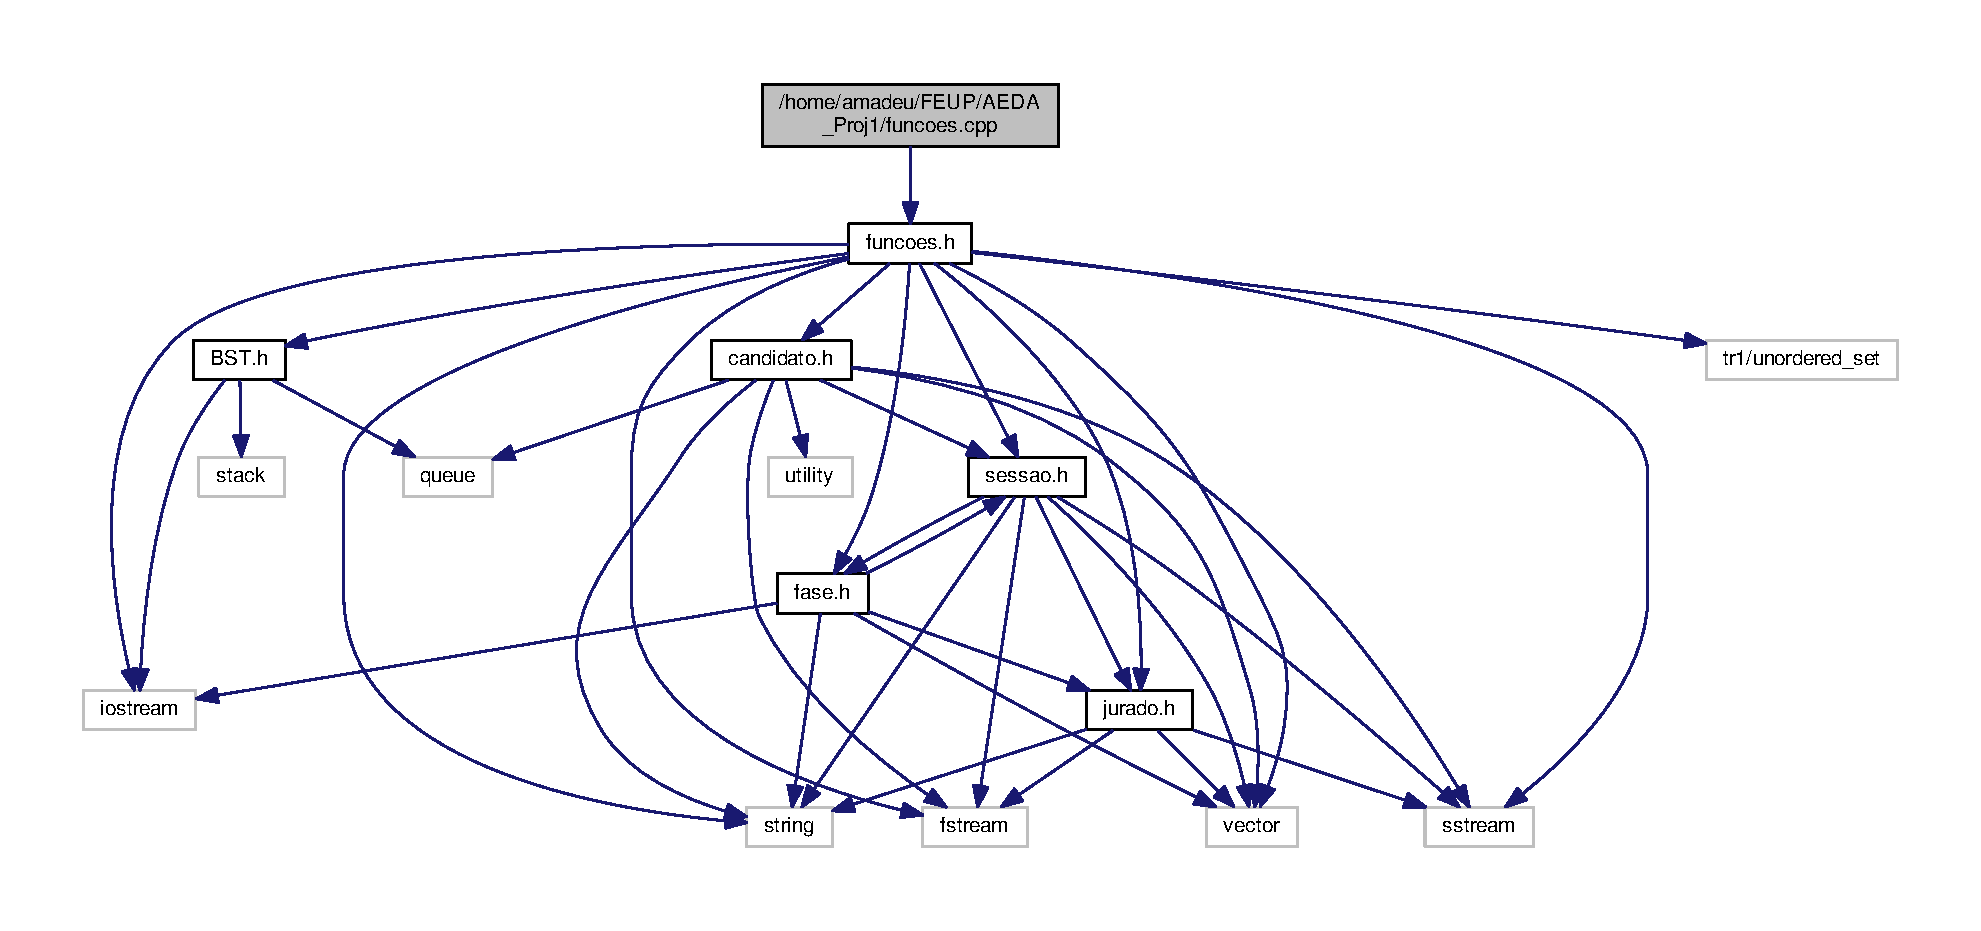
\includegraphics[width=350pt]{funcoes_8cpp__incl}
\end{center}
\end{figure}
\subsection*{Functions}
\begin{DoxyCompactItemize}
\item 
void \hyperlink{funcoes_8cpp_a35728269fe38e432b3dd133e78b1fd55}{reset\+Hash\+Table} ()
\begin{DoxyCompactList}\small\item\em remove todos os participantes exceto os que desistiram \end{DoxyCompactList}\item 
int \hyperlink{funcoes_8cpp_a03e271bb3bedf66f73cad262e700e837}{cin\+Teste} ()
\begin{DoxyCompactList}\small\item\em verifica se houve erro com o cin \end{DoxyCompactList}\item 
int \hyperlink{funcoes_8cpp_a7335042b18e3855974159d4d08c7a7c2}{ler\+Ficheiro\+Candidatos} ()
\begin{DoxyCompactList}\small\item\em lê o ficheiro e guarda a informacao dos candidatos no vetor global \end{DoxyCompactList}\item 
int \hyperlink{funcoes_8cpp_a80dac83ba60f597f6db8e22bc77a4de5}{ler\+Ficheiro\+Jurados} ()
\begin{DoxyCompactList}\small\item\em lê o ficheiro e guarda a informacao dos jurados no vetor global \end{DoxyCompactList}\item 
int \hyperlink{funcoes_8cpp_aa7a3938e939446fca96abf52819ec5aa}{ler\+Ficheiro\+Sessoes} ()
\begin{DoxyCompactList}\small\item\em lê o ficheiro e guarda a informacao das sessoes no vetor global \end{DoxyCompactList}\item 
int \hyperlink{funcoes_8cpp_a527d2f397f0c48b910095588a4c9187f}{ler\+Ficheiros} ()
\begin{DoxyCompactList}\small\item\em abre e lê a informacao de todos os ficheiros \end{DoxyCompactList}\item 
int \hyperlink{funcoes_8cpp_aedd438ee191a5d0073b0df5cebee5c06}{gravar\+Ficheiro\+Candidatos} ()
\begin{DoxyCompactList}\small\item\em grava o vetor global de candidatos no ficheiro \end{DoxyCompactList}\item 
int \hyperlink{funcoes_8cpp_a26b225e88f861652f753c3c302918fb9}{gravar\+Ficheiro\+Jurados} ()
\begin{DoxyCompactList}\small\item\em grava o vetor global de jurados no ficheiro \end{DoxyCompactList}\item 
int \hyperlink{funcoes_8cpp_a3dbb90e9800c11416d6aae34fd3efd09}{gravar\+Ficheiro\+Sessoes} ()
\begin{DoxyCompactList}\small\item\em grava o vetor global de sessoes no ficheiro \end{DoxyCompactList}\item 
int \hyperlink{funcoes_8cpp_af65e43314768eb1b18c8ea72b7db53c0}{gravar\+Ficheiros} ()
\begin{DoxyCompactList}\small\item\em grava os vetores globais nos ficheiros respetivos \end{DoxyCompactList}\item 
void \hyperlink{funcoes_8cpp_a26ac37d614dfa527c7b053d7cad26950}{sair} ()
\begin{DoxyCompactList}\small\item\em guarda informacao nos ficheiros e sair do programa \end{DoxyCompactList}\item 
void \hyperlink{funcoes_8cpp_ad766ed2d22fd7718188d925c228c0500}{adiciona\+Candidato} (\hyperlink{classcandidato}{candidato} c)
\begin{DoxyCompactList}\small\item\em adiciona um candidato \end{DoxyCompactList}\item 
void \hyperlink{funcoes_8cpp_a38b128fc1a8cf5839e81d632909177e2}{remove\+Candidato} (int numero)
\begin{DoxyCompactList}\small\item\em remove um candidato \end{DoxyCompactList}\item 
void \hyperlink{funcoes_8cpp_a6ae25de891ba5684070171585c468c58}{remove\+Candidato} (string nome)
\begin{DoxyCompactList}\small\item\em remove um candidato \end{DoxyCompactList}\item 
void \hyperlink{funcoes_8cpp_a3f9ae6c2a2f873eafba5dcf2a90812db}{alterar\+Candidato} (int numero)
\begin{DoxyCompactList}\small\item\em altera as informacoes de um candidato \end{DoxyCompactList}\item 
void \hyperlink{funcoes_8cpp_a17e7c5e32e7e7498dbb912bf9e834e61}{alterar\+Candidato} (string nome)
\begin{DoxyCompactList}\small\item\em altera as informacoes de um candidato \end{DoxyCompactList}\item 
void \hyperlink{funcoes_8cpp_a0eaa629e9fa2d0a368034d9d51755926}{info\+Candidato} (int numero)
\begin{DoxyCompactList}\small\item\em dá display da informacao do candidato \end{DoxyCompactList}\item 
void \hyperlink{funcoes_8cpp_aad9e9cc84f293130064cf9484adff5ac}{info\+Candidato} (\hyperlink{classcandidato}{candidato} c)
\begin{DoxyCompactList}\small\item\em dá display da informacao do candidato \end{DoxyCompactList}\item 
void \hyperlink{funcoes_8cpp_aed1a3b47f489be1e24c3b3173ae3ca77}{adiciona\+Jurado} (\hyperlink{classjurado}{jurado} $\ast$j)
\begin{DoxyCompactList}\small\item\em adiciona um jurado \end{DoxyCompactList}\item 
void \hyperlink{funcoes_8cpp_a977fecb61bbc152ce7760ba950b0a3eb}{remove\+Jurado} (string nome)
\begin{DoxyCompactList}\small\item\em remove um jurado \end{DoxyCompactList}\item 
void \hyperlink{funcoes_8cpp_ab228dd12131d805687f5efc999be740d}{info\+Jurado} (string nome)
\begin{DoxyCompactList}\small\item\em dá display da informacao do jurado \end{DoxyCompactList}\item 
void \hyperlink{funcoes_8cpp_a6d5358f6ddfef6e930f443c71dcd7deb}{info\+Jurado} (\hyperlink{classjurado}{jurado} $\ast$j)
\begin{DoxyCompactList}\small\item\em dá display da informacao dos jurados \end{DoxyCompactList}\item 
\hyperlink{classBSTItrIn}{B\+S\+T\+Itr\+In}$<$ \hyperlink{classcandidato}{candidato} $>$ \hyperlink{funcoes_8cpp_a0b55c14ba666b441a4c6f0dd0509fbfa}{procura\+Candidato} (\hyperlink{classcandidato}{candidato} c)
\begin{DoxyCompactList}\small\item\em procura se o candidato se encontra no vetor global \end{DoxyCompactList}\item 
\hyperlink{classBSTItrIn}{B\+S\+T\+Itr\+In}$<$ \hyperlink{classcandidato}{candidato} $>$ \hyperlink{funcoes_8cpp_aa96b384c150d783ed651baaba395e163}{procura\+Candidato} (int numero)
\begin{DoxyCompactList}\small\item\em procura se o candidato se encontra no vetor global \end{DoxyCompactList}\item 
\hyperlink{classBSTItrIn}{B\+S\+T\+Itr\+In}$<$ \hyperlink{classcandidato}{candidato} $>$ \hyperlink{funcoes_8cpp_a428152cfce79ff13931b60019771e87e}{procura\+Candidato} (string nome)
\begin{DoxyCompactList}\small\item\em procura se o candidato se encontra no vetor global \end{DoxyCompactList}\item 
int \hyperlink{funcoes_8cpp_ae538da495cdcf7c84535390216211e8f}{procura\+Jurado} (\hyperlink{classjurado}{jurado} $\ast$j)
\begin{DoxyCompactList}\small\item\em procura se o jurado se encontra no vetor global de jurados \end{DoxyCompactList}\item 
int \hyperlink{funcoes_8cpp_aa63ed5266b677ed47f735e26e5be010e}{procura\+Jurado} (string nome)
\begin{DoxyCompactList}\small\item\em procura se o jurado se encontra no vetor global de jurados \end{DoxyCompactList}\item 
int \hyperlink{funcoes_8cpp_a950f2dc53b3249b8665c1b0d673b0926}{procura\+Sessao} (string genero\+Arte, vector$<$ int $>$ data)
\begin{DoxyCompactList}\small\item\em procura se a sessao se encontra no vetor global de sessoes \end{DoxyCompactList}\item 
int \hyperlink{funcoes_8cpp_a28991002c5dfdf06508b236d60709d92}{procura\+Sessao} (\hyperlink{classsessao}{sessao} $\ast$s)
\begin{DoxyCompactList}\small\item\em procura se a sessao se encontra no vetor global de sessoes \end{DoxyCompactList}\item 
void \hyperlink{funcoes_8cpp_ac8fe930867cdb0d85a9d1d1aa045da6f}{adiciona\+Sessao} (\hyperlink{classsessao}{sessao} $\ast$s)
\begin{DoxyCompactList}\small\item\em adiciona uma nova sessao ao vetor global sessoes \end{DoxyCompactList}\item 
void \hyperlink{funcoes_8cpp_a1c106f754a83de93d9aedd564d768437}{remove\+Sessao} (string genero\+Arte, vector$<$ int $>$ data)
\begin{DoxyCompactList}\small\item\em remove uma sessao do vetor global de sessoes \end{DoxyCompactList}\item 
void \hyperlink{funcoes_8cpp_a62b097f473c1a672a3fdf1555d32350f}{remove\+Fases} (\hyperlink{classsessao}{sessao} $\ast$s)
\begin{DoxyCompactList}\small\item\em remove as fases de uma sessao \end{DoxyCompactList}\item 
vector$<$ int $>$ \hyperlink{funcoes_8cpp_abf7dc8ccb49b447a01758b49417be421}{candidatos\+Disponiveis} (\hyperlink{classsessao}{sessao} $\ast$s)
\begin{DoxyCompactList}\small\item\em da display de todos os candidatos disponiveis para uma sessao \end{DoxyCompactList}\item 
vector$<$ string $>$ \hyperlink{funcoes_8cpp_a0405cae70c2d8ef83f45114e549f8231}{jurados\+Disponiveis} (\hyperlink{classsessao}{sessao} $\ast$s)
\begin{DoxyCompactList}\small\item\em da display de todos os jurados disponiveis para uma sessao \end{DoxyCompactList}\item 
void \hyperlink{funcoes_8cpp_a78b13210272a9a59830544851d9b955e}{adiciona\+Candidato\+Sessao} (int n, \hyperlink{classsessao}{sessao} $\ast$s)
\begin{DoxyCompactList}\small\item\em adiciona um candidato a uma sessao \end{DoxyCompactList}\item 
void \hyperlink{funcoes_8cpp_a157d29cdc4b75416540f6a577cb8a2e1}{adiciona\+Jurado\+Sessao} (string nome, \hyperlink{classsessao}{sessao} $\ast$s)
\begin{DoxyCompactList}\small\item\em adiciona um jurado a uma sessao \end{DoxyCompactList}\item 
void \hyperlink{funcoes_8cpp_a0d910f3431d1acf2a513ed93c336699e}{display\+Info\+Sessao} (string arte, vector$<$ int $>$ data)
\begin{DoxyCompactList}\small\item\em dá display das informacoes de uma sessao \end{DoxyCompactList}\item 
void \hyperlink{funcoes_8cpp_ab6074f9624a6827c4a74e48cd114f12a}{comecar\+Sessao} (string arte, vector$<$ int $>$ data)
\begin{DoxyCompactList}\small\item\em esta funcao permite a atribuicao de pontos a cada candidato de uma sessao (para ambas as fases) mostrando no fim o vencedor tambem adiciona aos vetores globais as novas fases \end{DoxyCompactList}\item 
int \hyperlink{funcoes_8cpp_a6d8972b532c33ef140f35dc19f476caa}{procura\+Fase1} (\hyperlink{classsessao}{sessao} $\ast$s)
\begin{DoxyCompactList}\small\item\em procura se a sessao ja tem uma \hyperlink{classfase1}{fase1} \end{DoxyCompactList}\item 
int \hyperlink{funcoes_8cpp_a1f254fcf857e05f9adbd28e2c144ac14}{procura\+Fase2} (\hyperlink{classsessao}{sessao} $\ast$s)
\begin{DoxyCompactList}\small\item\em procura se a sessao ja tem uma \hyperlink{classfase2}{fase2} \end{DoxyCompactList}\end{DoxyCompactItemize}
\subsection*{Variables}
\begin{DoxyCompactItemize}
\item 
\hyperlink{classcandidato}{candidato} \hyperlink{funcoes_8cpp_a4577f0625a9cb11baf4f0c481fc463c5}{notF} = \hyperlink{classcandidato}{candidato}()
\item 
\hyperlink{classBST}{B\+ST}$<$ \hyperlink{classcandidato}{candidato} $>$ \hyperlink{funcoes_8cpp_a84f115e3fbf17c018b4746eb95ac1b5a}{candidatos\+Global} (\hyperlink{funcoes_8h_a4577f0625a9cb11baf4f0c481fc463c5}{notF})
\item 
vector$<$ \hyperlink{classjurado}{jurado} $\ast$ $>$ \hyperlink{funcoes_8cpp_ae9435e6e661379e8e415046d02a346fa}{jurados\+Global}
\item 
vector$<$ \hyperlink{classsessao}{sessao} $\ast$ $>$ \hyperlink{funcoes_8cpp_a8d719244453f7f8ffad19bbf9a61379e}{sessao\+Global}
\item 
vector$<$ \hyperlink{classfase1}{fase1} $>$ \hyperlink{funcoes_8cpp_a6c049f7ef530d38d2ec88ab69c691ec9}{fases1}
\item 
vector$<$ \hyperlink{classfase2}{fase2} $>$ \hyperlink{funcoes_8cpp_a8dbf01c38737187aa4a624bfa435940f}{fases2}
\item 
\hyperlink{funcoes_8h_ac8c2773477a4703c8516077e593542b6}{Hash\+Tab} \hyperlink{funcoes_8cpp_ac7f4b498c121dea87209cfe06252a444}{indisponibilidades}
\end{DoxyCompactItemize}


\subsection{Function Documentation}
\index{funcoes.\+cpp@{funcoes.\+cpp}!adiciona\+Candidato@{adiciona\+Candidato}}
\index{adiciona\+Candidato@{adiciona\+Candidato}!funcoes.\+cpp@{funcoes.\+cpp}}
\subsubsection[{\texorpdfstring{adiciona\+Candidato(candidato c)}{adicionaCandidato(candidato c)}}]{\setlength{\rightskip}{0pt plus 5cm}void adiciona\+Candidato (
\begin{DoxyParamCaption}
\item[{{\bf candidato}}]{c}
\end{DoxyParamCaption}
)}\hypertarget{funcoes_8cpp_ad766ed2d22fd7718188d925c228c0500}{}\label{funcoes_8cpp_ad766ed2d22fd7718188d925c228c0500}


adiciona um candidato 


\begin{DoxyParams}{Parameters}
{\em c} & objeto de um candidato \\
\hline
\end{DoxyParams}
\index{funcoes.\+cpp@{funcoes.\+cpp}!adiciona\+Candidato\+Sessao@{adiciona\+Candidato\+Sessao}}
\index{adiciona\+Candidato\+Sessao@{adiciona\+Candidato\+Sessao}!funcoes.\+cpp@{funcoes.\+cpp}}
\subsubsection[{\texorpdfstring{adiciona\+Candidato\+Sessao(int n, sessao $\ast$s)}{adicionaCandidatoSessao(int n, sessao *s)}}]{\setlength{\rightskip}{0pt plus 5cm}void adiciona\+Candidato\+Sessao (
\begin{DoxyParamCaption}
\item[{int}]{n, }
\item[{{\bf sessao} $\ast$}]{s}
\end{DoxyParamCaption}
)}\hypertarget{funcoes_8cpp_a78b13210272a9a59830544851d9b955e}{}\label{funcoes_8cpp_a78b13210272a9a59830544851d9b955e}


adiciona um candidato a uma sessao 


\begin{DoxyParams}{Parameters}
{\em n} & numero do candidato \\
\hline
{\em s} & sessao a adicionar \\
\hline
\end{DoxyParams}
\index{funcoes.\+cpp@{funcoes.\+cpp}!adiciona\+Jurado@{adiciona\+Jurado}}
\index{adiciona\+Jurado@{adiciona\+Jurado}!funcoes.\+cpp@{funcoes.\+cpp}}
\subsubsection[{\texorpdfstring{adiciona\+Jurado(jurado $\ast$j)}{adicionaJurado(jurado *j)}}]{\setlength{\rightskip}{0pt plus 5cm}void adiciona\+Jurado (
\begin{DoxyParamCaption}
\item[{{\bf jurado} $\ast$}]{j}
\end{DoxyParamCaption}
)}\hypertarget{funcoes_8cpp_aed1a3b47f489be1e24c3b3173ae3ca77}{}\label{funcoes_8cpp_aed1a3b47f489be1e24c3b3173ae3ca77}


adiciona um jurado 


\begin{DoxyParams}{Parameters}
{\em j} & objeto de um jurado \\
\hline
\end{DoxyParams}
\index{funcoes.\+cpp@{funcoes.\+cpp}!adiciona\+Jurado\+Sessao@{adiciona\+Jurado\+Sessao}}
\index{adiciona\+Jurado\+Sessao@{adiciona\+Jurado\+Sessao}!funcoes.\+cpp@{funcoes.\+cpp}}
\subsubsection[{\texorpdfstring{adiciona\+Jurado\+Sessao(string nome, sessao $\ast$s)}{adicionaJuradoSessao(string nome, sessao *s)}}]{\setlength{\rightskip}{0pt plus 5cm}void adiciona\+Jurado\+Sessao (
\begin{DoxyParamCaption}
\item[{string}]{nome, }
\item[{{\bf sessao} $\ast$}]{s}
\end{DoxyParamCaption}
)}\hypertarget{funcoes_8cpp_a157d29cdc4b75416540f6a577cb8a2e1}{}\label{funcoes_8cpp_a157d29cdc4b75416540f6a577cb8a2e1}


adiciona um jurado a uma sessao 


\begin{DoxyParams}{Parameters}
{\em nome} & nome do jurado \\
\hline
{\em s} & sessao a adicionar \\
\hline
\end{DoxyParams}
\index{funcoes.\+cpp@{funcoes.\+cpp}!adiciona\+Sessao@{adiciona\+Sessao}}
\index{adiciona\+Sessao@{adiciona\+Sessao}!funcoes.\+cpp@{funcoes.\+cpp}}
\subsubsection[{\texorpdfstring{adiciona\+Sessao(sessao $\ast$s)}{adicionaSessao(sessao *s)}}]{\setlength{\rightskip}{0pt plus 5cm}void adiciona\+Sessao (
\begin{DoxyParamCaption}
\item[{{\bf sessao} $\ast$}]{s}
\end{DoxyParamCaption}
)}\hypertarget{funcoes_8cpp_ac8fe930867cdb0d85a9d1d1aa045da6f}{}\label{funcoes_8cpp_ac8fe930867cdb0d85a9d1d1aa045da6f}


adiciona uma nova sessao ao vetor global sessoes 


\begin{DoxyParams}{Parameters}
{\em s} & sessao a adicionar \\
\hline
\end{DoxyParams}
\index{funcoes.\+cpp@{funcoes.\+cpp}!alterar\+Candidato@{alterar\+Candidato}}
\index{alterar\+Candidato@{alterar\+Candidato}!funcoes.\+cpp@{funcoes.\+cpp}}
\subsubsection[{\texorpdfstring{alterar\+Candidato(int numero)}{alterarCandidato(int numero)}}]{\setlength{\rightskip}{0pt plus 5cm}void alterar\+Candidato (
\begin{DoxyParamCaption}
\item[{int}]{numero}
\end{DoxyParamCaption}
)}\hypertarget{funcoes_8cpp_a3f9ae6c2a2f873eafba5dcf2a90812db}{}\label{funcoes_8cpp_a3f9ae6c2a2f873eafba5dcf2a90812db}


altera as informacoes de um candidato 


\begin{DoxyParams}{Parameters}
{\em numero} & numero do candidato a alterar \\
\hline
\end{DoxyParams}
\index{funcoes.\+cpp@{funcoes.\+cpp}!alterar\+Candidato@{alterar\+Candidato}}
\index{alterar\+Candidato@{alterar\+Candidato}!funcoes.\+cpp@{funcoes.\+cpp}}
\subsubsection[{\texorpdfstring{alterar\+Candidato(string nome)}{alterarCandidato(string nome)}}]{\setlength{\rightskip}{0pt plus 5cm}void alterar\+Candidato (
\begin{DoxyParamCaption}
\item[{string}]{nome}
\end{DoxyParamCaption}
)}\hypertarget{funcoes_8cpp_a17e7c5e32e7e7498dbb912bf9e834e61}{}\label{funcoes_8cpp_a17e7c5e32e7e7498dbb912bf9e834e61}


altera as informacoes de um candidato 


\begin{DoxyParams}{Parameters}
{\em nome} & nome do candidato a alterar \\
\hline
\end{DoxyParams}
\index{funcoes.\+cpp@{funcoes.\+cpp}!candidatos\+Disponiveis@{candidatos\+Disponiveis}}
\index{candidatos\+Disponiveis@{candidatos\+Disponiveis}!funcoes.\+cpp@{funcoes.\+cpp}}
\subsubsection[{\texorpdfstring{candidatos\+Disponiveis(sessao $\ast$s)}{candidatosDisponiveis(sessao *s)}}]{\setlength{\rightskip}{0pt plus 5cm}vector$<$int$>$ candidatos\+Disponiveis (
\begin{DoxyParamCaption}
\item[{{\bf sessao} $\ast$}]{s}
\end{DoxyParamCaption}
)}\hypertarget{funcoes_8cpp_abf7dc8ccb49b447a01758b49417be421}{}\label{funcoes_8cpp_abf7dc8ccb49b447a01758b49417be421}


da display de todos os candidatos disponiveis para uma sessao 


\begin{DoxyParams}{Parameters}
{\em s} & sessao a analisar \\
\hline
\end{DoxyParams}
\begin{DoxyReturn}{Returns}
vector com os numeros de todos os candidatos disponiveis 
\end{DoxyReturn}
\index{funcoes.\+cpp@{funcoes.\+cpp}!cin\+Teste@{cin\+Teste}}
\index{cin\+Teste@{cin\+Teste}!funcoes.\+cpp@{funcoes.\+cpp}}
\subsubsection[{\texorpdfstring{cin\+Teste()}{cinTeste()}}]{\setlength{\rightskip}{0pt plus 5cm}int cin\+Teste (
\begin{DoxyParamCaption}
{}
\end{DoxyParamCaption}
)}\hypertarget{funcoes_8cpp_a03e271bb3bedf66f73cad262e700e837}{}\label{funcoes_8cpp_a03e271bb3bedf66f73cad262e700e837}


verifica se houve erro com o cin 

\begin{DoxyReturn}{Returns}
0 nao houve erro, 1 se houve erro 
\end{DoxyReturn}
\index{funcoes.\+cpp@{funcoes.\+cpp}!comecar\+Sessao@{comecar\+Sessao}}
\index{comecar\+Sessao@{comecar\+Sessao}!funcoes.\+cpp@{funcoes.\+cpp}}
\subsubsection[{\texorpdfstring{comecar\+Sessao(string arte, vector$<$ int $>$ data)}{comecarSessao(string arte, vector< int > data)}}]{\setlength{\rightskip}{0pt plus 5cm}void comecar\+Sessao (
\begin{DoxyParamCaption}
\item[{string}]{arte, }
\item[{vector$<$ int $>$}]{data}
\end{DoxyParamCaption}
)}\hypertarget{funcoes_8cpp_ab6074f9624a6827c4a74e48cd114f12a}{}\label{funcoes_8cpp_ab6074f9624a6827c4a74e48cd114f12a}


esta funcao permite a atribuicao de pontos a cada candidato de uma sessao (para ambas as fases) mostrando no fim o vencedor tambem adiciona aos vetores globais as novas fases 


\begin{DoxyParams}{Parameters}
{\em arte} & a arte da sessao \\
\hline
{\em data} & a data da sessao \\
\hline
\end{DoxyParams}
\index{funcoes.\+cpp@{funcoes.\+cpp}!display\+Info\+Sessao@{display\+Info\+Sessao}}
\index{display\+Info\+Sessao@{display\+Info\+Sessao}!funcoes.\+cpp@{funcoes.\+cpp}}
\subsubsection[{\texorpdfstring{display\+Info\+Sessao(string arte, vector$<$ int $>$ data)}{displayInfoSessao(string arte, vector< int > data)}}]{\setlength{\rightskip}{0pt plus 5cm}void display\+Info\+Sessao (
\begin{DoxyParamCaption}
\item[{string}]{arte, }
\item[{vector$<$ int $>$}]{data}
\end{DoxyParamCaption}
)}\hypertarget{funcoes_8cpp_a0d910f3431d1acf2a513ed93c336699e}{}\label{funcoes_8cpp_a0d910f3431d1acf2a513ed93c336699e}


dá display das informacoes de uma sessao 


\begin{DoxyParams}{Parameters}
{\em arte} & arte da sessao \\
\hline
{\em data} & data da sessao \\
\hline
\end{DoxyParams}
\index{funcoes.\+cpp@{funcoes.\+cpp}!gravar\+Ficheiro\+Candidatos@{gravar\+Ficheiro\+Candidatos}}
\index{gravar\+Ficheiro\+Candidatos@{gravar\+Ficheiro\+Candidatos}!funcoes.\+cpp@{funcoes.\+cpp}}
\subsubsection[{\texorpdfstring{gravar\+Ficheiro\+Candidatos()}{gravarFicheiroCandidatos()}}]{\setlength{\rightskip}{0pt plus 5cm}int gravar\+Ficheiro\+Candidatos (
\begin{DoxyParamCaption}
{}
\end{DoxyParamCaption}
)}\hypertarget{funcoes_8cpp_aedd438ee191a5d0073b0df5cebee5c06}{}\label{funcoes_8cpp_aedd438ee191a5d0073b0df5cebee5c06}


grava o vetor global de candidatos no ficheiro 

\begin{DoxyReturn}{Returns}
0 se sucesso, 1 se endereço invalido 
\end{DoxyReturn}
\index{funcoes.\+cpp@{funcoes.\+cpp}!gravar\+Ficheiro\+Jurados@{gravar\+Ficheiro\+Jurados}}
\index{gravar\+Ficheiro\+Jurados@{gravar\+Ficheiro\+Jurados}!funcoes.\+cpp@{funcoes.\+cpp}}
\subsubsection[{\texorpdfstring{gravar\+Ficheiro\+Jurados()}{gravarFicheiroJurados()}}]{\setlength{\rightskip}{0pt plus 5cm}int gravar\+Ficheiro\+Jurados (
\begin{DoxyParamCaption}
{}
\end{DoxyParamCaption}
)}\hypertarget{funcoes_8cpp_a26b225e88f861652f753c3c302918fb9}{}\label{funcoes_8cpp_a26b225e88f861652f753c3c302918fb9}


grava o vetor global de jurados no ficheiro 

\begin{DoxyReturn}{Returns}
0 se sucesso, 1 se endereço invalido 
\end{DoxyReturn}
\index{funcoes.\+cpp@{funcoes.\+cpp}!gravar\+Ficheiros@{gravar\+Ficheiros}}
\index{gravar\+Ficheiros@{gravar\+Ficheiros}!funcoes.\+cpp@{funcoes.\+cpp}}
\subsubsection[{\texorpdfstring{gravar\+Ficheiros()}{gravarFicheiros()}}]{\setlength{\rightskip}{0pt plus 5cm}int gravar\+Ficheiros (
\begin{DoxyParamCaption}
{}
\end{DoxyParamCaption}
)}\hypertarget{funcoes_8cpp_af65e43314768eb1b18c8ea72b7db53c0}{}\label{funcoes_8cpp_af65e43314768eb1b18c8ea72b7db53c0}


grava os vetores globais nos ficheiros respetivos 

\begin{DoxyReturn}{Returns}
0 se nao houver erro, 1 se houver erro 
\end{DoxyReturn}
\index{funcoes.\+cpp@{funcoes.\+cpp}!gravar\+Ficheiro\+Sessoes@{gravar\+Ficheiro\+Sessoes}}
\index{gravar\+Ficheiro\+Sessoes@{gravar\+Ficheiro\+Sessoes}!funcoes.\+cpp@{funcoes.\+cpp}}
\subsubsection[{\texorpdfstring{gravar\+Ficheiro\+Sessoes()}{gravarFicheiroSessoes()}}]{\setlength{\rightskip}{0pt plus 5cm}int gravar\+Ficheiro\+Sessoes (
\begin{DoxyParamCaption}
{}
\end{DoxyParamCaption}
)}\hypertarget{funcoes_8cpp_a3dbb90e9800c11416d6aae34fd3efd09}{}\label{funcoes_8cpp_a3dbb90e9800c11416d6aae34fd3efd09}


grava o vetor global de sessoes no ficheiro 

\begin{DoxyReturn}{Returns}
0 se sucesso, 1 se endereço invalido 
\end{DoxyReturn}
\index{funcoes.\+cpp@{funcoes.\+cpp}!info\+Candidato@{info\+Candidato}}
\index{info\+Candidato@{info\+Candidato}!funcoes.\+cpp@{funcoes.\+cpp}}
\subsubsection[{\texorpdfstring{info\+Candidato(int numero)}{infoCandidato(int numero)}}]{\setlength{\rightskip}{0pt plus 5cm}void info\+Candidato (
\begin{DoxyParamCaption}
\item[{int}]{numero}
\end{DoxyParamCaption}
)}\hypertarget{funcoes_8cpp_a0eaa629e9fa2d0a368034d9d51755926}{}\label{funcoes_8cpp_a0eaa629e9fa2d0a368034d9d51755926}


dá display da informacao do candidato 


\begin{DoxyParams}{Parameters}
{\em numero} & numero do candidato \\
\hline
\end{DoxyParams}
\index{funcoes.\+cpp@{funcoes.\+cpp}!info\+Candidato@{info\+Candidato}}
\index{info\+Candidato@{info\+Candidato}!funcoes.\+cpp@{funcoes.\+cpp}}
\subsubsection[{\texorpdfstring{info\+Candidato(candidato c)}{infoCandidato(candidato c)}}]{\setlength{\rightskip}{0pt plus 5cm}void info\+Candidato (
\begin{DoxyParamCaption}
\item[{{\bf candidato}}]{c}
\end{DoxyParamCaption}
)}\hypertarget{funcoes_8cpp_aad9e9cc84f293130064cf9484adff5ac}{}\label{funcoes_8cpp_aad9e9cc84f293130064cf9484adff5ac}


dá display da informacao do candidato 


\begin{DoxyParams}{Parameters}
{\em c} & candidato pretendido \\
\hline
\end{DoxyParams}
\index{funcoes.\+cpp@{funcoes.\+cpp}!info\+Jurado@{info\+Jurado}}
\index{info\+Jurado@{info\+Jurado}!funcoes.\+cpp@{funcoes.\+cpp}}
\subsubsection[{\texorpdfstring{info\+Jurado(string nome)}{infoJurado(string nome)}}]{\setlength{\rightskip}{0pt plus 5cm}void info\+Jurado (
\begin{DoxyParamCaption}
\item[{string}]{nome}
\end{DoxyParamCaption}
)}\hypertarget{funcoes_8cpp_ab228dd12131d805687f5efc999be740d}{}\label{funcoes_8cpp_ab228dd12131d805687f5efc999be740d}


dá display da informacao do jurado 


\begin{DoxyParams}{Parameters}
{\em nome} & nome do jurado \\
\hline
\end{DoxyParams}
\index{funcoes.\+cpp@{funcoes.\+cpp}!info\+Jurado@{info\+Jurado}}
\index{info\+Jurado@{info\+Jurado}!funcoes.\+cpp@{funcoes.\+cpp}}
\subsubsection[{\texorpdfstring{info\+Jurado(jurado $\ast$j)}{infoJurado(jurado *j)}}]{\setlength{\rightskip}{0pt plus 5cm}void info\+Jurado (
\begin{DoxyParamCaption}
\item[{{\bf jurado} $\ast$}]{j}
\end{DoxyParamCaption}
)}\hypertarget{funcoes_8cpp_a6d5358f6ddfef6e930f443c71dcd7deb}{}\label{funcoes_8cpp_a6d5358f6ddfef6e930f443c71dcd7deb}


dá display da informacao dos jurados 


\begin{DoxyParams}{Parameters}
{\em j} & objecto de um jurado \\
\hline
\end{DoxyParams}
\index{funcoes.\+cpp@{funcoes.\+cpp}!jurados\+Disponiveis@{jurados\+Disponiveis}}
\index{jurados\+Disponiveis@{jurados\+Disponiveis}!funcoes.\+cpp@{funcoes.\+cpp}}
\subsubsection[{\texorpdfstring{jurados\+Disponiveis(sessao $\ast$s)}{juradosDisponiveis(sessao *s)}}]{\setlength{\rightskip}{0pt plus 5cm}vector$<$string$>$ jurados\+Disponiveis (
\begin{DoxyParamCaption}
\item[{{\bf sessao} $\ast$}]{s}
\end{DoxyParamCaption}
)}\hypertarget{funcoes_8cpp_a0405cae70c2d8ef83f45114e549f8231}{}\label{funcoes_8cpp_a0405cae70c2d8ef83f45114e549f8231}


da display de todos os jurados disponiveis para uma sessao 


\begin{DoxyParams}{Parameters}
{\em s} & sessao a analisar \\
\hline
\end{DoxyParams}
\begin{DoxyReturn}{Returns}
vector com os nomes de todos os jurados disponiveis 
\end{DoxyReturn}
\index{funcoes.\+cpp@{funcoes.\+cpp}!ler\+Ficheiro\+Candidatos@{ler\+Ficheiro\+Candidatos}}
\index{ler\+Ficheiro\+Candidatos@{ler\+Ficheiro\+Candidatos}!funcoes.\+cpp@{funcoes.\+cpp}}
\subsubsection[{\texorpdfstring{ler\+Ficheiro\+Candidatos()}{lerFicheiroCandidatos()}}]{\setlength{\rightskip}{0pt plus 5cm}int ler\+Ficheiro\+Candidatos (
\begin{DoxyParamCaption}
{}
\end{DoxyParamCaption}
)}\hypertarget{funcoes_8cpp_a7335042b18e3855974159d4d08c7a7c2}{}\label{funcoes_8cpp_a7335042b18e3855974159d4d08c7a7c2}


lê o ficheiro e guarda a informacao dos candidatos no vetor global 

\begin{DoxyReturn}{Returns}
0 se sucesso, 1 se endereço invalido 
\end{DoxyReturn}
\index{funcoes.\+cpp@{funcoes.\+cpp}!ler\+Ficheiro\+Jurados@{ler\+Ficheiro\+Jurados}}
\index{ler\+Ficheiro\+Jurados@{ler\+Ficheiro\+Jurados}!funcoes.\+cpp@{funcoes.\+cpp}}
\subsubsection[{\texorpdfstring{ler\+Ficheiro\+Jurados()}{lerFicheiroJurados()}}]{\setlength{\rightskip}{0pt plus 5cm}int ler\+Ficheiro\+Jurados (
\begin{DoxyParamCaption}
{}
\end{DoxyParamCaption}
)}\hypertarget{funcoes_8cpp_a80dac83ba60f597f6db8e22bc77a4de5}{}\label{funcoes_8cpp_a80dac83ba60f597f6db8e22bc77a4de5}


lê o ficheiro e guarda a informacao dos jurados no vetor global 

\begin{DoxyReturn}{Returns}
0 se sucesso, 1 se endereço invalido 
\end{DoxyReturn}
\index{funcoes.\+cpp@{funcoes.\+cpp}!ler\+Ficheiros@{ler\+Ficheiros}}
\index{ler\+Ficheiros@{ler\+Ficheiros}!funcoes.\+cpp@{funcoes.\+cpp}}
\subsubsection[{\texorpdfstring{ler\+Ficheiros()}{lerFicheiros()}}]{\setlength{\rightskip}{0pt plus 5cm}int ler\+Ficheiros (
\begin{DoxyParamCaption}
{}
\end{DoxyParamCaption}
)}\hypertarget{funcoes_8cpp_a527d2f397f0c48b910095588a4c9187f}{}\label{funcoes_8cpp_a527d2f397f0c48b910095588a4c9187f}


abre e lê a informacao de todos os ficheiros 

\begin{DoxyReturn}{Returns}
0 se nao houver erro, 1 se houve algum erro 
\end{DoxyReturn}
\index{funcoes.\+cpp@{funcoes.\+cpp}!ler\+Ficheiro\+Sessoes@{ler\+Ficheiro\+Sessoes}}
\index{ler\+Ficheiro\+Sessoes@{ler\+Ficheiro\+Sessoes}!funcoes.\+cpp@{funcoes.\+cpp}}
\subsubsection[{\texorpdfstring{ler\+Ficheiro\+Sessoes()}{lerFicheiroSessoes()}}]{\setlength{\rightskip}{0pt plus 5cm}int ler\+Ficheiro\+Sessoes (
\begin{DoxyParamCaption}
{}
\end{DoxyParamCaption}
)}\hypertarget{funcoes_8cpp_aa7a3938e939446fca96abf52819ec5aa}{}\label{funcoes_8cpp_aa7a3938e939446fca96abf52819ec5aa}


lê o ficheiro e guarda a informacao das sessoes no vetor global 

\begin{DoxyReturn}{Returns}
0 se sucesso, 1 se endereço invalido 
\end{DoxyReturn}
\index{funcoes.\+cpp@{funcoes.\+cpp}!procura\+Candidato@{procura\+Candidato}}
\index{procura\+Candidato@{procura\+Candidato}!funcoes.\+cpp@{funcoes.\+cpp}}
\subsubsection[{\texorpdfstring{procura\+Candidato(candidato c)}{procuraCandidato(candidato c)}}]{\setlength{\rightskip}{0pt plus 5cm}{\bf B\+S\+T\+Itr\+In}$<${\bf candidato}$>$ procura\+Candidato (
\begin{DoxyParamCaption}
\item[{{\bf candidato}}]{c}
\end{DoxyParamCaption}
)}\hypertarget{funcoes_8cpp_a0b55c14ba666b441a4c6f0dd0509fbfa}{}\label{funcoes_8cpp_a0b55c14ba666b441a4c6f0dd0509fbfa}


procura se o candidato se encontra no vetor global 


\begin{DoxyParams}{Parameters}
{\em c} & candidato a procurar \\
\hline
\end{DoxyParams}
\begin{DoxyReturn}{Returns}
iterador 
\end{DoxyReturn}
\index{funcoes.\+cpp@{funcoes.\+cpp}!procura\+Candidato@{procura\+Candidato}}
\index{procura\+Candidato@{procura\+Candidato}!funcoes.\+cpp@{funcoes.\+cpp}}
\subsubsection[{\texorpdfstring{procura\+Candidato(int numero)}{procuraCandidato(int numero)}}]{\setlength{\rightskip}{0pt plus 5cm}{\bf B\+S\+T\+Itr\+In}$<${\bf candidato}$>$ procura\+Candidato (
\begin{DoxyParamCaption}
\item[{int}]{numero}
\end{DoxyParamCaption}
)}\hypertarget{funcoes_8cpp_aa96b384c150d783ed651baaba395e163}{}\label{funcoes_8cpp_aa96b384c150d783ed651baaba395e163}


procura se o candidato se encontra no vetor global 


\begin{DoxyParams}{Parameters}
{\em numero} & numero do candidato a procurar \\
\hline
\end{DoxyParams}
\begin{DoxyReturn}{Returns}
iterador 
\end{DoxyReturn}
\index{funcoes.\+cpp@{funcoes.\+cpp}!procura\+Candidato@{procura\+Candidato}}
\index{procura\+Candidato@{procura\+Candidato}!funcoes.\+cpp@{funcoes.\+cpp}}
\subsubsection[{\texorpdfstring{procura\+Candidato(string nome)}{procuraCandidato(string nome)}}]{\setlength{\rightskip}{0pt plus 5cm}{\bf B\+S\+T\+Itr\+In}$<${\bf candidato}$>$ procura\+Candidato (
\begin{DoxyParamCaption}
\item[{string}]{nome}
\end{DoxyParamCaption}
)}\hypertarget{funcoes_8cpp_a428152cfce79ff13931b60019771e87e}{}\label{funcoes_8cpp_a428152cfce79ff13931b60019771e87e}


procura se o candidato se encontra no vetor global 


\begin{DoxyParams}{Parameters}
{\em nome} & nome do candidato a procurar \\
\hline
\end{DoxyParams}
\begin{DoxyReturn}{Returns}
iterador 
\end{DoxyReturn}
\index{funcoes.\+cpp@{funcoes.\+cpp}!procura\+Fase1@{procura\+Fase1}}
\index{procura\+Fase1@{procura\+Fase1}!funcoes.\+cpp@{funcoes.\+cpp}}
\subsubsection[{\texorpdfstring{procura\+Fase1(sessao $\ast$s)}{procuraFase1(sessao *s)}}]{\setlength{\rightskip}{0pt plus 5cm}int procura\+Fase1 (
\begin{DoxyParamCaption}
\item[{{\bf sessao} $\ast$}]{s}
\end{DoxyParamCaption}
)}\hypertarget{funcoes_8cpp_a6d8972b532c33ef140f35dc19f476caa}{}\label{funcoes_8cpp_a6d8972b532c33ef140f35dc19f476caa}


procura se a sessao ja tem uma \hyperlink{classfase1}{fase1} 


\begin{DoxyParams}{Parameters}
{\em s} & sessao a procurar \\
\hline
\end{DoxyParams}
\begin{DoxyReturn}{Returns}
indice da fase se existir , -\/1 caso contrário 
\end{DoxyReturn}
\index{funcoes.\+cpp@{funcoes.\+cpp}!procura\+Fase2@{procura\+Fase2}}
\index{procura\+Fase2@{procura\+Fase2}!funcoes.\+cpp@{funcoes.\+cpp}}
\subsubsection[{\texorpdfstring{procura\+Fase2(sessao $\ast$s)}{procuraFase2(sessao *s)}}]{\setlength{\rightskip}{0pt plus 5cm}int procura\+Fase2 (
\begin{DoxyParamCaption}
\item[{{\bf sessao} $\ast$}]{s}
\end{DoxyParamCaption}
)}\hypertarget{funcoes_8cpp_a1f254fcf857e05f9adbd28e2c144ac14}{}\label{funcoes_8cpp_a1f254fcf857e05f9adbd28e2c144ac14}


procura se a sessao ja tem uma \hyperlink{classfase2}{fase2} 


\begin{DoxyParams}{Parameters}
{\em s} & sessao a procurar \\
\hline
\end{DoxyParams}
\begin{DoxyReturn}{Returns}
indice da fase se existir , -\/1 caso contrário 
\end{DoxyReturn}
\index{funcoes.\+cpp@{funcoes.\+cpp}!procura\+Jurado@{procura\+Jurado}}
\index{procura\+Jurado@{procura\+Jurado}!funcoes.\+cpp@{funcoes.\+cpp}}
\subsubsection[{\texorpdfstring{procura\+Jurado(jurado $\ast$j)}{procuraJurado(jurado *j)}}]{\setlength{\rightskip}{0pt plus 5cm}int procura\+Jurado (
\begin{DoxyParamCaption}
\item[{{\bf jurado} $\ast$}]{c}
\end{DoxyParamCaption}
)}\hypertarget{funcoes_8cpp_ae538da495cdcf7c84535390216211e8f}{}\label{funcoes_8cpp_ae538da495cdcf7c84535390216211e8f}


procura se o jurado se encontra no vetor global de jurados 


\begin{DoxyParams}{Parameters}
{\em j} & jurado a procurar \\
\hline
\end{DoxyParams}
\begin{DoxyReturn}{Returns}
indice se existir , -\/1 caso contrário 
\end{DoxyReturn}
\index{funcoes.\+cpp@{funcoes.\+cpp}!procura\+Jurado@{procura\+Jurado}}
\index{procura\+Jurado@{procura\+Jurado}!funcoes.\+cpp@{funcoes.\+cpp}}
\subsubsection[{\texorpdfstring{procura\+Jurado(string nome)}{procuraJurado(string nome)}}]{\setlength{\rightskip}{0pt plus 5cm}int procura\+Jurado (
\begin{DoxyParamCaption}
\item[{string}]{nome}
\end{DoxyParamCaption}
)}\hypertarget{funcoes_8cpp_aa63ed5266b677ed47f735e26e5be010e}{}\label{funcoes_8cpp_aa63ed5266b677ed47f735e26e5be010e}


procura se o jurado se encontra no vetor global de jurados 


\begin{DoxyParams}{Parameters}
{\em nome} & nome do jurado a procurar \\
\hline
\end{DoxyParams}
\begin{DoxyReturn}{Returns}
indice se existir , -\/1 caso contrário 
\end{DoxyReturn}
\index{funcoes.\+cpp@{funcoes.\+cpp}!procura\+Sessao@{procura\+Sessao}}
\index{procura\+Sessao@{procura\+Sessao}!funcoes.\+cpp@{funcoes.\+cpp}}
\subsubsection[{\texorpdfstring{procura\+Sessao(string genero\+Arte, vector$<$ int $>$ data)}{procuraSessao(string generoArte, vector< int > data)}}]{\setlength{\rightskip}{0pt plus 5cm}int procura\+Sessao (
\begin{DoxyParamCaption}
\item[{string}]{genero\+Arte, }
\item[{vector$<$ int $>$}]{data}
\end{DoxyParamCaption}
)}\hypertarget{funcoes_8cpp_a950f2dc53b3249b8665c1b0d673b0926}{}\label{funcoes_8cpp_a950f2dc53b3249b8665c1b0d673b0926}


procura se a sessao se encontra no vetor global de sessoes 


\begin{DoxyParams}{Parameters}
{\em s} & genero\+Arte é o genero de arte da sessao pretendida \\
\hline
{\em data} & é da data da sessao \\
\hline
\end{DoxyParams}
\begin{DoxyReturn}{Returns}
indice se existir , -\/1 caso contrário 
\end{DoxyReturn}
\index{funcoes.\+cpp@{funcoes.\+cpp}!procura\+Sessao@{procura\+Sessao}}
\index{procura\+Sessao@{procura\+Sessao}!funcoes.\+cpp@{funcoes.\+cpp}}
\subsubsection[{\texorpdfstring{procura\+Sessao(sessao $\ast$s)}{procuraSessao(sessao *s)}}]{\setlength{\rightskip}{0pt plus 5cm}int procura\+Sessao (
\begin{DoxyParamCaption}
\item[{{\bf sessao} $\ast$}]{s}
\end{DoxyParamCaption}
)}\hypertarget{funcoes_8cpp_a28991002c5dfdf06508b236d60709d92}{}\label{funcoes_8cpp_a28991002c5dfdf06508b236d60709d92}


procura se a sessao se encontra no vetor global de sessoes 


\begin{DoxyParams}{Parameters}
{\em s} & sessao a procurar \\
\hline
\end{DoxyParams}
\begin{DoxyReturn}{Returns}
indice se existir , -\/1 caso contrário 
\end{DoxyReturn}
\index{funcoes.\+cpp@{funcoes.\+cpp}!remove\+Candidato@{remove\+Candidato}}
\index{remove\+Candidato@{remove\+Candidato}!funcoes.\+cpp@{funcoes.\+cpp}}
\subsubsection[{\texorpdfstring{remove\+Candidato(int numero)}{removeCandidato(int numero)}}]{\setlength{\rightskip}{0pt plus 5cm}void remove\+Candidato (
\begin{DoxyParamCaption}
\item[{int}]{numero}
\end{DoxyParamCaption}
)}\hypertarget{funcoes_8cpp_a38b128fc1a8cf5839e81d632909177e2}{}\label{funcoes_8cpp_a38b128fc1a8cf5839e81d632909177e2}


remove um candidato 


\begin{DoxyParams}{Parameters}
{\em numero} & numero do candidato a remover \\
\hline
\end{DoxyParams}
\index{funcoes.\+cpp@{funcoes.\+cpp}!remove\+Candidato@{remove\+Candidato}}
\index{remove\+Candidato@{remove\+Candidato}!funcoes.\+cpp@{funcoes.\+cpp}}
\subsubsection[{\texorpdfstring{remove\+Candidato(string nome)}{removeCandidato(string nome)}}]{\setlength{\rightskip}{0pt plus 5cm}void remove\+Candidato (
\begin{DoxyParamCaption}
\item[{string}]{nome}
\end{DoxyParamCaption}
)}\hypertarget{funcoes_8cpp_a6ae25de891ba5684070171585c468c58}{}\label{funcoes_8cpp_a6ae25de891ba5684070171585c468c58}


remove um candidato 


\begin{DoxyParams}{Parameters}
{\em nome} & nome do candidato a remover \\
\hline
\end{DoxyParams}
\index{funcoes.\+cpp@{funcoes.\+cpp}!remove\+Fases@{remove\+Fases}}
\index{remove\+Fases@{remove\+Fases}!funcoes.\+cpp@{funcoes.\+cpp}}
\subsubsection[{\texorpdfstring{remove\+Fases(sessao $\ast$s)}{removeFases(sessao *s)}}]{\setlength{\rightskip}{0pt plus 5cm}void remove\+Fases (
\begin{DoxyParamCaption}
\item[{{\bf sessao} $\ast$}]{s}
\end{DoxyParamCaption}
)}\hypertarget{funcoes_8cpp_a62b097f473c1a672a3fdf1555d32350f}{}\label{funcoes_8cpp_a62b097f473c1a672a3fdf1555d32350f}


remove as fases de uma sessao 


\begin{DoxyParams}{Parameters}
{\em s} & sessao \\
\hline
\end{DoxyParams}
\index{funcoes.\+cpp@{funcoes.\+cpp}!remove\+Jurado@{remove\+Jurado}}
\index{remove\+Jurado@{remove\+Jurado}!funcoes.\+cpp@{funcoes.\+cpp}}
\subsubsection[{\texorpdfstring{remove\+Jurado(string nome)}{removeJurado(string nome)}}]{\setlength{\rightskip}{0pt plus 5cm}void remove\+Jurado (
\begin{DoxyParamCaption}
\item[{string}]{nome}
\end{DoxyParamCaption}
)}\hypertarget{funcoes_8cpp_a977fecb61bbc152ce7760ba950b0a3eb}{}\label{funcoes_8cpp_a977fecb61bbc152ce7760ba950b0a3eb}


remove um jurado 


\begin{DoxyParams}{Parameters}
{\em nome} & nome do jurado a remover \\
\hline
\end{DoxyParams}
\index{funcoes.\+cpp@{funcoes.\+cpp}!remove\+Sessao@{remove\+Sessao}}
\index{remove\+Sessao@{remove\+Sessao}!funcoes.\+cpp@{funcoes.\+cpp}}
\subsubsection[{\texorpdfstring{remove\+Sessao(string genero\+Arte, vector$<$ int $>$ data)}{removeSessao(string generoArte, vector< int > data)}}]{\setlength{\rightskip}{0pt plus 5cm}void remove\+Sessao (
\begin{DoxyParamCaption}
\item[{string}]{genero\+Arte, }
\item[{vector$<$ int $>$}]{data}
\end{DoxyParamCaption}
)}\hypertarget{funcoes_8cpp_a1c106f754a83de93d9aedd564d768437}{}\label{funcoes_8cpp_a1c106f754a83de93d9aedd564d768437}


remove uma sessao do vetor global de sessoes 


\begin{DoxyParams}{Parameters}
{\em genero\+Arte} & generto de arte da sessao a remover \\
\hline
{\em data} & vetor com a data (dia,mes,ano) a remover \\
\hline
\end{DoxyParams}
\index{funcoes.\+cpp@{funcoes.\+cpp}!reset\+Hash\+Table@{reset\+Hash\+Table}}
\index{reset\+Hash\+Table@{reset\+Hash\+Table}!funcoes.\+cpp@{funcoes.\+cpp}}
\subsubsection[{\texorpdfstring{reset\+Hash\+Table()}{resetHashTable()}}]{\setlength{\rightskip}{0pt plus 5cm}void reset\+Hash\+Table (
\begin{DoxyParamCaption}
{}
\end{DoxyParamCaption}
)}\hypertarget{funcoes_8cpp_a35728269fe38e432b3dd133e78b1fd55}{}\label{funcoes_8cpp_a35728269fe38e432b3dd133e78b1fd55}


remove todos os participantes exceto os que desistiram 

\index{funcoes.\+cpp@{funcoes.\+cpp}!sair@{sair}}
\index{sair@{sair}!funcoes.\+cpp@{funcoes.\+cpp}}
\subsubsection[{\texorpdfstring{sair()}{sair()}}]{\setlength{\rightskip}{0pt plus 5cm}void sair (
\begin{DoxyParamCaption}
{}
\end{DoxyParamCaption}
)}\hypertarget{funcoes_8cpp_a26ac37d614dfa527c7b053d7cad26950}{}\label{funcoes_8cpp_a26ac37d614dfa527c7b053d7cad26950}


guarda informacao nos ficheiros e sair do programa 



\subsection{Variable Documentation}
\index{funcoes.\+cpp@{funcoes.\+cpp}!candidatos\+Global@{candidatos\+Global}}
\index{candidatos\+Global@{candidatos\+Global}!funcoes.\+cpp@{funcoes.\+cpp}}
\subsubsection[{\texorpdfstring{candidatos\+Global}{candidatosGlobal}}]{\setlength{\rightskip}{0pt plus 5cm}{\bf B\+ST}$<${\bf candidato}$>$ candidatos\+Global({\bf notF})}\hypertarget{funcoes_8cpp_a84f115e3fbf17c018b4746eb95ac1b5a}{}\label{funcoes_8cpp_a84f115e3fbf17c018b4746eb95ac1b5a}
\index{funcoes.\+cpp@{funcoes.\+cpp}!fases1@{fases1}}
\index{fases1@{fases1}!funcoes.\+cpp@{funcoes.\+cpp}}
\subsubsection[{\texorpdfstring{fases1}{fases1}}]{\setlength{\rightskip}{0pt plus 5cm}vector$<${\bf fase1}$>$ fases1}\hypertarget{funcoes_8cpp_a6c049f7ef530d38d2ec88ab69c691ec9}{}\label{funcoes_8cpp_a6c049f7ef530d38d2ec88ab69c691ec9}
\index{funcoes.\+cpp@{funcoes.\+cpp}!fases2@{fases2}}
\index{fases2@{fases2}!funcoes.\+cpp@{funcoes.\+cpp}}
\subsubsection[{\texorpdfstring{fases2}{fases2}}]{\setlength{\rightskip}{0pt plus 5cm}vector$<${\bf fase2}$>$ fases2}\hypertarget{funcoes_8cpp_a8dbf01c38737187aa4a624bfa435940f}{}\label{funcoes_8cpp_a8dbf01c38737187aa4a624bfa435940f}
\index{funcoes.\+cpp@{funcoes.\+cpp}!indisponibilidades@{indisponibilidades}}
\index{indisponibilidades@{indisponibilidades}!funcoes.\+cpp@{funcoes.\+cpp}}
\subsubsection[{\texorpdfstring{indisponibilidades}{indisponibilidades}}]{\setlength{\rightskip}{0pt plus 5cm}{\bf Hash\+Tab} indisponibilidades}\hypertarget{funcoes_8cpp_ac7f4b498c121dea87209cfe06252a444}{}\label{funcoes_8cpp_ac7f4b498c121dea87209cfe06252a444}
\index{funcoes.\+cpp@{funcoes.\+cpp}!jurados\+Global@{jurados\+Global}}
\index{jurados\+Global@{jurados\+Global}!funcoes.\+cpp@{funcoes.\+cpp}}
\subsubsection[{\texorpdfstring{jurados\+Global}{juradosGlobal}}]{\setlength{\rightskip}{0pt plus 5cm}vector$<${\bf jurado}$\ast$$>$ jurados\+Global}\hypertarget{funcoes_8cpp_ae9435e6e661379e8e415046d02a346fa}{}\label{funcoes_8cpp_ae9435e6e661379e8e415046d02a346fa}
\index{funcoes.\+cpp@{funcoes.\+cpp}!notF@{notF}}
\index{notF@{notF}!funcoes.\+cpp@{funcoes.\+cpp}}
\subsubsection[{\texorpdfstring{notF}{notF}}]{\setlength{\rightskip}{0pt plus 5cm}{\bf candidato} notF = {\bf candidato}()}\hypertarget{funcoes_8cpp_a4577f0625a9cb11baf4f0c481fc463c5}{}\label{funcoes_8cpp_a4577f0625a9cb11baf4f0c481fc463c5}
\index{funcoes.\+cpp@{funcoes.\+cpp}!sessao\+Global@{sessao\+Global}}
\index{sessao\+Global@{sessao\+Global}!funcoes.\+cpp@{funcoes.\+cpp}}
\subsubsection[{\texorpdfstring{sessao\+Global}{sessaoGlobal}}]{\setlength{\rightskip}{0pt plus 5cm}vector$<${\bf sessao}$\ast$$>$ sessao\+Global}\hypertarget{funcoes_8cpp_a8d719244453f7f8ffad19bbf9a61379e}{}\label{funcoes_8cpp_a8d719244453f7f8ffad19bbf9a61379e}

\hypertarget{funcoes_8h}{}\section{/home/amadeu/\+F\+E\+U\+P/\+A\+E\+D\+A\+\_\+\+Proj1/funcoes.h File Reference}
\label{funcoes_8h}\index{/home/amadeu/\+F\+E\+U\+P/\+A\+E\+D\+A\+\_\+\+Proj1/funcoes.\+h@{/home/amadeu/\+F\+E\+U\+P/\+A\+E\+D\+A\+\_\+\+Proj1/funcoes.\+h}}
{\ttfamily \#include $<$iostream$>$}\\*
{\ttfamily \#include $<$fstream$>$}\\*
{\ttfamily \#include $<$sstream$>$}\\*
{\ttfamily \#include $<$vector$>$}\\*
{\ttfamily \#include $<$string$>$}\\*
{\ttfamily \#include $<$tr1/unordered\+\_\+set$>$}\\*
{\ttfamily \#include \char`\"{}B\+S\+T.\+h\char`\"{}}\\*
{\ttfamily \#include \char`\"{}candidato.\+h\char`\"{}}\\*
{\ttfamily \#include \char`\"{}jurado.\+h\char`\"{}}\\*
{\ttfamily \#include \char`\"{}sessao.\+h\char`\"{}}\\*
{\ttfamily \#include \char`\"{}fase.\+h\char`\"{}}\\*
Include dependency graph for funcoes.\+h\+:
\nopagebreak
\begin{figure}[H]
\begin{center}
\leavevmode
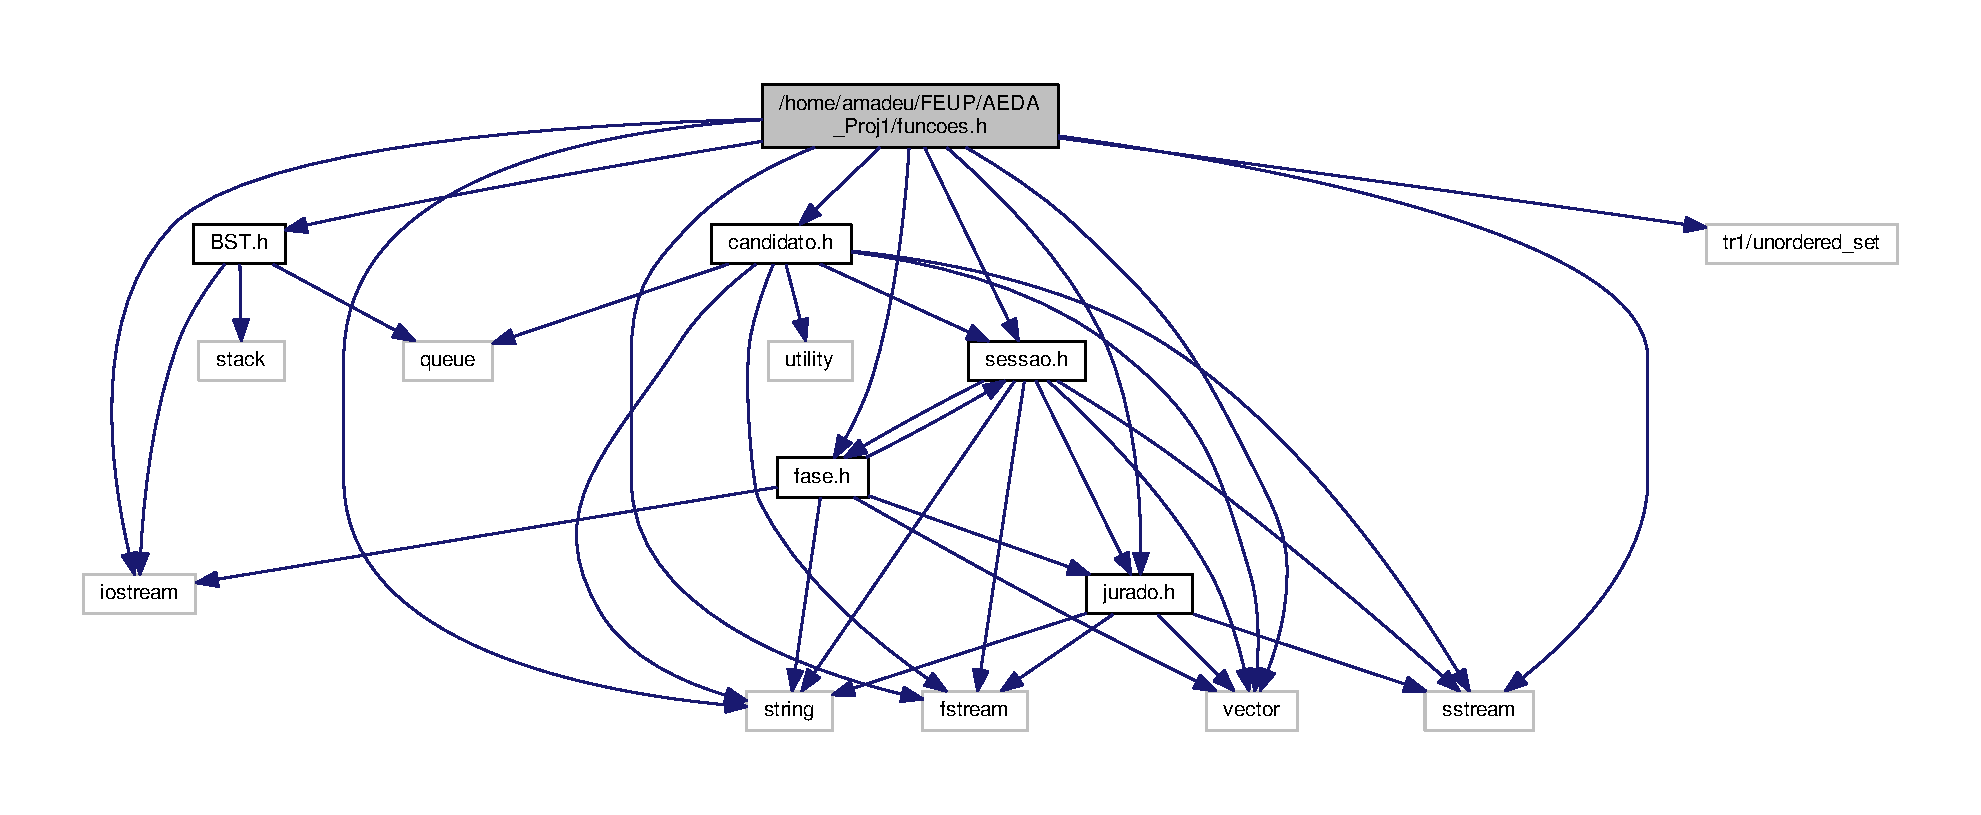
\includegraphics[width=350pt]{funcoes_8h__incl}
\end{center}
\end{figure}
This graph shows which files directly or indirectly include this file\+:
\nopagebreak
\begin{figure}[H]
\begin{center}
\leavevmode
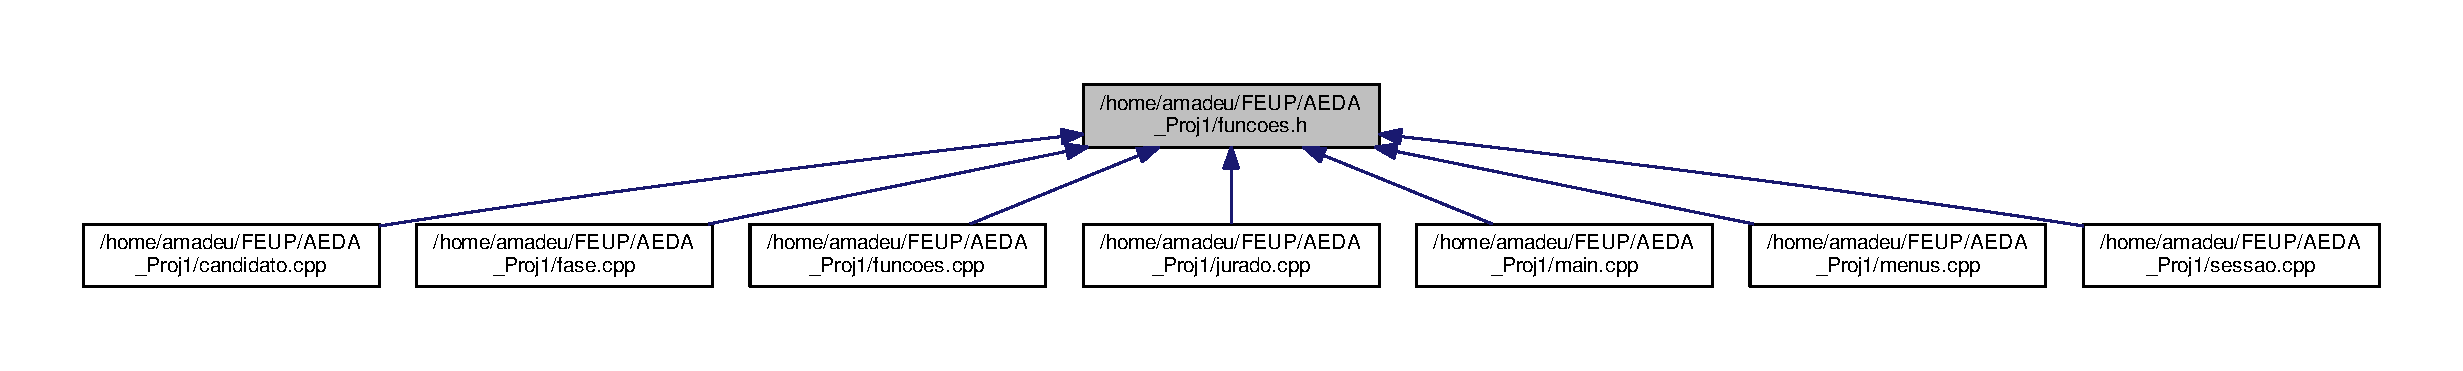
\includegraphics[width=350pt]{funcoes_8h__dep__incl}
\end{center}
\end{figure}
\subsection*{Classes}
\begin{DoxyCompactItemize}
\item 
struct \hyperlink{structh}{h}
\item 
struct \hyperlink{structeq}{eq}
\end{DoxyCompactItemize}
\subsection*{Typedefs}
\begin{DoxyCompactItemize}
\item 
typedef tr1\+::unordered\+\_\+set$<$ pair$<$ \hyperlink{classcandidato}{candidato}, string $>$, \hyperlink{structh}{h}, \hyperlink{structeq}{eq} $>$ \hyperlink{funcoes_8h_ac8c2773477a4703c8516077e593542b6}{Hash\+Tab}
\end{DoxyCompactItemize}
\subsection*{Functions}
\begin{DoxyCompactItemize}
\item 
void \hyperlink{funcoes_8h_a35728269fe38e432b3dd133e78b1fd55}{reset\+Hash\+Table} ()
\begin{DoxyCompactList}\small\item\em remove todos os participantes exceto os que desistiram \end{DoxyCompactList}\item 
int \hyperlink{funcoes_8h_a03e271bb3bedf66f73cad262e700e837}{cin\+Teste} ()
\begin{DoxyCompactList}\small\item\em verifica se houve erro com o cin \end{DoxyCompactList}\item 
int \hyperlink{funcoes_8h_aedd438ee191a5d0073b0df5cebee5c06}{gravar\+Ficheiro\+Candidatos} ()
\begin{DoxyCompactList}\small\item\em grava o vetor global de candidatos no ficheiro \end{DoxyCompactList}\item 
int \hyperlink{funcoes_8h_a26b225e88f861652f753c3c302918fb9}{gravar\+Ficheiro\+Jurados} ()
\begin{DoxyCompactList}\small\item\em grava o vetor global de jurados no ficheiro \end{DoxyCompactList}\item 
int \hyperlink{funcoes_8h_a3dbb90e9800c11416d6aae34fd3efd09}{gravar\+Ficheiro\+Sessoes} ()
\begin{DoxyCompactList}\small\item\em grava o vetor global de sessoes no ficheiro \end{DoxyCompactList}\item 
int \hyperlink{funcoes_8h_af65e43314768eb1b18c8ea72b7db53c0}{gravar\+Ficheiros} ()
\begin{DoxyCompactList}\small\item\em grava os vetores globais nos ficheiros respetivos \end{DoxyCompactList}\item 
int \hyperlink{funcoes_8h_a527d2f397f0c48b910095588a4c9187f}{ler\+Ficheiros} ()
\begin{DoxyCompactList}\small\item\em abre e lê a informacao de todos os ficheiros \end{DoxyCompactList}\item 
int \hyperlink{funcoes_8h_a7335042b18e3855974159d4d08c7a7c2}{ler\+Ficheiro\+Candidatos} ()
\begin{DoxyCompactList}\small\item\em lê o ficheiro e guarda a informacao dos candidatos no vetor global \end{DoxyCompactList}\item 
int \hyperlink{funcoes_8h_a80dac83ba60f597f6db8e22bc77a4de5}{ler\+Ficheiro\+Jurados} ()
\begin{DoxyCompactList}\small\item\em lê o ficheiro e guarda a informacao dos jurados no vetor global \end{DoxyCompactList}\item 
int \hyperlink{funcoes_8h_aa7a3938e939446fca96abf52819ec5aa}{ler\+Ficheiro\+Sessoes} ()
\begin{DoxyCompactList}\small\item\em lê o ficheiro e guarda a informacao das sessoes no vetor global \end{DoxyCompactList}\item 
void \hyperlink{funcoes_8h_a26ac37d614dfa527c7b053d7cad26950}{sair} ()
\begin{DoxyCompactList}\small\item\em guarda informacao nos ficheiros e sair do programa \end{DoxyCompactList}\item 
void \hyperlink{funcoes_8h_ad766ed2d22fd7718188d925c228c0500}{adiciona\+Candidato} (\hyperlink{classcandidato}{candidato} c)
\begin{DoxyCompactList}\small\item\em adiciona um candidato \end{DoxyCompactList}\item 
void \hyperlink{funcoes_8h_a38b128fc1a8cf5839e81d632909177e2}{remove\+Candidato} (int numero)
\begin{DoxyCompactList}\small\item\em remove um candidato \end{DoxyCompactList}\item 
void \hyperlink{funcoes_8h_a6ae25de891ba5684070171585c468c58}{remove\+Candidato} (string nome)
\begin{DoxyCompactList}\small\item\em remove um candidato \end{DoxyCompactList}\item 
void \hyperlink{funcoes_8h_a3f9ae6c2a2f873eafba5dcf2a90812db}{alterar\+Candidato} (int numero)
\begin{DoxyCompactList}\small\item\em altera as informacoes de um candidato \end{DoxyCompactList}\item 
void \hyperlink{funcoes_8h_a17e7c5e32e7e7498dbb912bf9e834e61}{alterar\+Candidato} (string nome)
\begin{DoxyCompactList}\small\item\em altera as informacoes de um candidato \end{DoxyCompactList}\item 
void \hyperlink{funcoes_8h_a0eaa629e9fa2d0a368034d9d51755926}{info\+Candidato} (int numero)
\begin{DoxyCompactList}\small\item\em dá display da informacao do candidato \end{DoxyCompactList}\item 
void \hyperlink{funcoes_8h_aad9e9cc84f293130064cf9484adff5ac}{info\+Candidato} (\hyperlink{classcandidato}{candidato} c)
\begin{DoxyCompactList}\small\item\em dá display da informacao do candidato \end{DoxyCompactList}\item 
void \hyperlink{funcoes_8h_aed1a3b47f489be1e24c3b3173ae3ca77}{adiciona\+Jurado} (\hyperlink{classjurado}{jurado} $\ast$j)
\begin{DoxyCompactList}\small\item\em adiciona um jurado \end{DoxyCompactList}\item 
void \hyperlink{funcoes_8h_a977fecb61bbc152ce7760ba950b0a3eb}{remove\+Jurado} (string nome)
\begin{DoxyCompactList}\small\item\em remove um jurado \end{DoxyCompactList}\item 
void \hyperlink{funcoes_8h_a6d5358f6ddfef6e930f443c71dcd7deb}{info\+Jurado} (\hyperlink{classjurado}{jurado} $\ast$j)
\begin{DoxyCompactList}\small\item\em dá display da informacao dos jurados \end{DoxyCompactList}\item 
\hyperlink{classBSTItrIn}{B\+S\+T\+Itr\+In}$<$ \hyperlink{classcandidato}{candidato} $>$ \hyperlink{funcoes_8h_a0b55c14ba666b441a4c6f0dd0509fbfa}{procura\+Candidato} (\hyperlink{classcandidato}{candidato} c)
\begin{DoxyCompactList}\small\item\em procura se o candidato se encontra no vetor global \end{DoxyCompactList}\item 
\hyperlink{classBSTItrIn}{B\+S\+T\+Itr\+In}$<$ \hyperlink{classcandidato}{candidato} $>$ \hyperlink{funcoes_8h_aa96b384c150d783ed651baaba395e163}{procura\+Candidato} (int numero)
\begin{DoxyCompactList}\small\item\em procura se o candidato se encontra no vetor global \end{DoxyCompactList}\item 
\hyperlink{classBSTItrIn}{B\+S\+T\+Itr\+In}$<$ \hyperlink{classcandidato}{candidato} $>$ \hyperlink{funcoes_8h_a428152cfce79ff13931b60019771e87e}{procura\+Candidato} (string nome)
\begin{DoxyCompactList}\small\item\em procura se o candidato se encontra no vetor global \end{DoxyCompactList}\item 
int \hyperlink{funcoes_8h_a57a0374c1a4df81b8083130574e7f05e}{procura\+Jurado} (\hyperlink{classjurado}{jurado} $\ast$c)
\begin{DoxyCompactList}\small\item\em procura se o jurado se encontra no vetor global de jurados \end{DoxyCompactList}\item 
int \hyperlink{funcoes_8h_aa63ed5266b677ed47f735e26e5be010e}{procura\+Jurado} (string nome)
\begin{DoxyCompactList}\small\item\em procura se o jurado se encontra no vetor global de jurados \end{DoxyCompactList}\item 
void \hyperlink{funcoes_8h_ab228dd12131d805687f5efc999be740d}{info\+Jurado} (string nome)
\begin{DoxyCompactList}\small\item\em dá display da informacao do jurado \end{DoxyCompactList}\item 
int \hyperlink{funcoes_8h_a28991002c5dfdf06508b236d60709d92}{procura\+Sessao} (\hyperlink{classsessao}{sessao} $\ast$s)
\begin{DoxyCompactList}\small\item\em procura se a sessao se encontra no vetor global de sessoes \end{DoxyCompactList}\item 
int \hyperlink{funcoes_8h_a950f2dc53b3249b8665c1b0d673b0926}{procura\+Sessao} (string genero\+Arte, vector$<$ int $>$ data)
\begin{DoxyCompactList}\small\item\em procura se a sessao se encontra no vetor global de sessoes \end{DoxyCompactList}\item 
void \hyperlink{funcoes_8h_ac8fe930867cdb0d85a9d1d1aa045da6f}{adiciona\+Sessao} (\hyperlink{classsessao}{sessao} $\ast$s)
\begin{DoxyCompactList}\small\item\em adiciona uma nova sessao ao vetor global sessoes \end{DoxyCompactList}\item 
void \hyperlink{funcoes_8h_a1c106f754a83de93d9aedd564d768437}{remove\+Sessao} (string genero\+Arte, vector$<$ int $>$ data)
\begin{DoxyCompactList}\small\item\em remove uma sessao do vetor global de sessoes \end{DoxyCompactList}\item 
vector$<$ int $>$ \hyperlink{funcoes_8h_abf7dc8ccb49b447a01758b49417be421}{candidatos\+Disponiveis} (\hyperlink{classsessao}{sessao} $\ast$s)
\begin{DoxyCompactList}\small\item\em da display de todos os candidatos disponiveis para uma sessao \end{DoxyCompactList}\item 
vector$<$ string $>$ \hyperlink{funcoes_8h_a0405cae70c2d8ef83f45114e549f8231}{jurados\+Disponiveis} (\hyperlink{classsessao}{sessao} $\ast$s)
\begin{DoxyCompactList}\small\item\em da display de todos os jurados disponiveis para uma sessao \end{DoxyCompactList}\item 
void \hyperlink{funcoes_8h_a78b13210272a9a59830544851d9b955e}{adiciona\+Candidato\+Sessao} (int n, \hyperlink{classsessao}{sessao} $\ast$s)
\begin{DoxyCompactList}\small\item\em adiciona um candidato a uma sessao \end{DoxyCompactList}\item 
void \hyperlink{funcoes_8h_a157d29cdc4b75416540f6a577cb8a2e1}{adiciona\+Jurado\+Sessao} (string nome, \hyperlink{classsessao}{sessao} $\ast$s)
\begin{DoxyCompactList}\small\item\em adiciona um jurado a uma sessao \end{DoxyCompactList}\item 
void \hyperlink{funcoes_8h_a0d910f3431d1acf2a513ed93c336699e}{display\+Info\+Sessao} (string arte, vector$<$ int $>$ data)
\begin{DoxyCompactList}\small\item\em dá display das informacoes de uma sessao \end{DoxyCompactList}\item 
void \hyperlink{funcoes_8h_ab6074f9624a6827c4a74e48cd114f12a}{comecar\+Sessao} (string arte, vector$<$ int $>$ data)
\begin{DoxyCompactList}\small\item\em esta funcao permite a atribuicao de pontos a cada candidato de uma sessao (para ambas as fases) mostrando no fim o vencedor tambem adiciona aos vetores globais as novas fases \end{DoxyCompactList}\item 
int \hyperlink{funcoes_8h_a6d8972b532c33ef140f35dc19f476caa}{procura\+Fase1} (\hyperlink{classsessao}{sessao} $\ast$s)
\begin{DoxyCompactList}\small\item\em procura se a sessao ja tem uma \hyperlink{classfase1}{fase1} \end{DoxyCompactList}\item 
int \hyperlink{funcoes_8h_a1f254fcf857e05f9adbd28e2c144ac14}{procura\+Fase2} (\hyperlink{classsessao}{sessao} $\ast$s)
\begin{DoxyCompactList}\small\item\em procura se a sessao ja tem uma \hyperlink{classfase2}{fase2} \end{DoxyCompactList}\item 
void \hyperlink{funcoes_8h_a62b097f473c1a672a3fdf1555d32350f}{remove\+Fases} (\hyperlink{classsessao}{sessao} $\ast$s)
\begin{DoxyCompactList}\small\item\em remove as fases de uma sessao \end{DoxyCompactList}\end{DoxyCompactItemize}
\subsection*{Variables}
\begin{DoxyCompactItemize}
\item 
\hyperlink{classcandidato}{candidato} \hyperlink{funcoes_8h_a4577f0625a9cb11baf4f0c481fc463c5}{notF}
\item 
\hyperlink{classBST}{B\+ST}$<$ \hyperlink{classcandidato}{candidato} $>$ \hyperlink{funcoes_8h_ad345338cd1a61dcea7a277e4fb323c9d}{candidatos\+Global}
\item 
vector$<$ \hyperlink{classjurado}{jurado} $\ast$ $>$ \hyperlink{funcoes_8h_ae9435e6e661379e8e415046d02a346fa}{jurados\+Global}
\item 
vector$<$ \hyperlink{classsessao}{sessao} $\ast$ $>$ \hyperlink{funcoes_8h_a8d719244453f7f8ffad19bbf9a61379e}{sessao\+Global}
\item 
vector$<$ \hyperlink{classfase1}{fase1} $>$ \hyperlink{funcoes_8h_a6c049f7ef530d38d2ec88ab69c691ec9}{fases1}
\item 
vector$<$ \hyperlink{classfase2}{fase2} $>$ \hyperlink{funcoes_8h_a8dbf01c38737187aa4a624bfa435940f}{fases2}
\item 
\hyperlink{funcoes_8h_ac8c2773477a4703c8516077e593542b6}{Hash\+Tab} \hyperlink{funcoes_8h_ac7f4b498c121dea87209cfe06252a444}{indisponibilidades}
\end{DoxyCompactItemize}


\subsection{Typedef Documentation}
\index{funcoes.\+h@{funcoes.\+h}!Hash\+Tab@{Hash\+Tab}}
\index{Hash\+Tab@{Hash\+Tab}!funcoes.\+h@{funcoes.\+h}}
\subsubsection[{\texorpdfstring{Hash\+Tab}{HashTab}}]{\setlength{\rightskip}{0pt plus 5cm}typedef tr1\+::unordered\+\_\+set$<$pair$<${\bf candidato}, string$>$, {\bf h}, {\bf eq}$>$ {\bf Hash\+Tab}}\hypertarget{funcoes_8h_ac8c2773477a4703c8516077e593542b6}{}\label{funcoes_8h_ac8c2773477a4703c8516077e593542b6}


\subsection{Function Documentation}
\index{funcoes.\+h@{funcoes.\+h}!adiciona\+Candidato@{adiciona\+Candidato}}
\index{adiciona\+Candidato@{adiciona\+Candidato}!funcoes.\+h@{funcoes.\+h}}
\subsubsection[{\texorpdfstring{adiciona\+Candidato(candidato c)}{adicionaCandidato(candidato c)}}]{\setlength{\rightskip}{0pt plus 5cm}void adiciona\+Candidato (
\begin{DoxyParamCaption}
\item[{{\bf candidato}}]{c}
\end{DoxyParamCaption}
)}\hypertarget{funcoes_8h_ad766ed2d22fd7718188d925c228c0500}{}\label{funcoes_8h_ad766ed2d22fd7718188d925c228c0500}


adiciona um candidato 


\begin{DoxyParams}{Parameters}
{\em c} & objeto de um candidato \\
\hline
\end{DoxyParams}
\index{funcoes.\+h@{funcoes.\+h}!adiciona\+Candidato\+Sessao@{adiciona\+Candidato\+Sessao}}
\index{adiciona\+Candidato\+Sessao@{adiciona\+Candidato\+Sessao}!funcoes.\+h@{funcoes.\+h}}
\subsubsection[{\texorpdfstring{adiciona\+Candidato\+Sessao(int n, sessao $\ast$s)}{adicionaCandidatoSessao(int n, sessao *s)}}]{\setlength{\rightskip}{0pt plus 5cm}void adiciona\+Candidato\+Sessao (
\begin{DoxyParamCaption}
\item[{int}]{n, }
\item[{{\bf sessao} $\ast$}]{s}
\end{DoxyParamCaption}
)}\hypertarget{funcoes_8h_a78b13210272a9a59830544851d9b955e}{}\label{funcoes_8h_a78b13210272a9a59830544851d9b955e}


adiciona um candidato a uma sessao 


\begin{DoxyParams}{Parameters}
{\em n} & numero do candidato \\
\hline
{\em s} & sessao a adicionar \\
\hline
\end{DoxyParams}
\index{funcoes.\+h@{funcoes.\+h}!adiciona\+Jurado@{adiciona\+Jurado}}
\index{adiciona\+Jurado@{adiciona\+Jurado}!funcoes.\+h@{funcoes.\+h}}
\subsubsection[{\texorpdfstring{adiciona\+Jurado(jurado $\ast$j)}{adicionaJurado(jurado *j)}}]{\setlength{\rightskip}{0pt plus 5cm}void adiciona\+Jurado (
\begin{DoxyParamCaption}
\item[{{\bf jurado} $\ast$}]{j}
\end{DoxyParamCaption}
)}\hypertarget{funcoes_8h_aed1a3b47f489be1e24c3b3173ae3ca77}{}\label{funcoes_8h_aed1a3b47f489be1e24c3b3173ae3ca77}


adiciona um jurado 


\begin{DoxyParams}{Parameters}
{\em j} & objeto de um jurado \\
\hline
\end{DoxyParams}
\index{funcoes.\+h@{funcoes.\+h}!adiciona\+Jurado\+Sessao@{adiciona\+Jurado\+Sessao}}
\index{adiciona\+Jurado\+Sessao@{adiciona\+Jurado\+Sessao}!funcoes.\+h@{funcoes.\+h}}
\subsubsection[{\texorpdfstring{adiciona\+Jurado\+Sessao(string nome, sessao $\ast$s)}{adicionaJuradoSessao(string nome, sessao *s)}}]{\setlength{\rightskip}{0pt plus 5cm}void adiciona\+Jurado\+Sessao (
\begin{DoxyParamCaption}
\item[{string}]{nome, }
\item[{{\bf sessao} $\ast$}]{s}
\end{DoxyParamCaption}
)}\hypertarget{funcoes_8h_a157d29cdc4b75416540f6a577cb8a2e1}{}\label{funcoes_8h_a157d29cdc4b75416540f6a577cb8a2e1}


adiciona um jurado a uma sessao 


\begin{DoxyParams}{Parameters}
{\em nome} & nome do jurado \\
\hline
{\em s} & sessao a adicionar \\
\hline
\end{DoxyParams}
\index{funcoes.\+h@{funcoes.\+h}!adiciona\+Sessao@{adiciona\+Sessao}}
\index{adiciona\+Sessao@{adiciona\+Sessao}!funcoes.\+h@{funcoes.\+h}}
\subsubsection[{\texorpdfstring{adiciona\+Sessao(sessao $\ast$s)}{adicionaSessao(sessao *s)}}]{\setlength{\rightskip}{0pt plus 5cm}void adiciona\+Sessao (
\begin{DoxyParamCaption}
\item[{{\bf sessao} $\ast$}]{s}
\end{DoxyParamCaption}
)}\hypertarget{funcoes_8h_ac8fe930867cdb0d85a9d1d1aa045da6f}{}\label{funcoes_8h_ac8fe930867cdb0d85a9d1d1aa045da6f}


adiciona uma nova sessao ao vetor global sessoes 


\begin{DoxyParams}{Parameters}
{\em s} & sessao a adicionar \\
\hline
\end{DoxyParams}
\index{funcoes.\+h@{funcoes.\+h}!alterar\+Candidato@{alterar\+Candidato}}
\index{alterar\+Candidato@{alterar\+Candidato}!funcoes.\+h@{funcoes.\+h}}
\subsubsection[{\texorpdfstring{alterar\+Candidato(int numero)}{alterarCandidato(int numero)}}]{\setlength{\rightskip}{0pt plus 5cm}void alterar\+Candidato (
\begin{DoxyParamCaption}
\item[{int}]{numero}
\end{DoxyParamCaption}
)}\hypertarget{funcoes_8h_a3f9ae6c2a2f873eafba5dcf2a90812db}{}\label{funcoes_8h_a3f9ae6c2a2f873eafba5dcf2a90812db}


altera as informacoes de um candidato 


\begin{DoxyParams}{Parameters}
{\em numero} & numero do candidato a alterar \\
\hline
\end{DoxyParams}
\index{funcoes.\+h@{funcoes.\+h}!alterar\+Candidato@{alterar\+Candidato}}
\index{alterar\+Candidato@{alterar\+Candidato}!funcoes.\+h@{funcoes.\+h}}
\subsubsection[{\texorpdfstring{alterar\+Candidato(string nome)}{alterarCandidato(string nome)}}]{\setlength{\rightskip}{0pt plus 5cm}void alterar\+Candidato (
\begin{DoxyParamCaption}
\item[{string}]{nome}
\end{DoxyParamCaption}
)}\hypertarget{funcoes_8h_a17e7c5e32e7e7498dbb912bf9e834e61}{}\label{funcoes_8h_a17e7c5e32e7e7498dbb912bf9e834e61}


altera as informacoes de um candidato 


\begin{DoxyParams}{Parameters}
{\em nome} & nome do candidato a alterar \\
\hline
\end{DoxyParams}
\index{funcoes.\+h@{funcoes.\+h}!candidatos\+Disponiveis@{candidatos\+Disponiveis}}
\index{candidatos\+Disponiveis@{candidatos\+Disponiveis}!funcoes.\+h@{funcoes.\+h}}
\subsubsection[{\texorpdfstring{candidatos\+Disponiveis(sessao $\ast$s)}{candidatosDisponiveis(sessao *s)}}]{\setlength{\rightskip}{0pt plus 5cm}vector$<$int$>$ candidatos\+Disponiveis (
\begin{DoxyParamCaption}
\item[{{\bf sessao} $\ast$}]{s}
\end{DoxyParamCaption}
)}\hypertarget{funcoes_8h_abf7dc8ccb49b447a01758b49417be421}{}\label{funcoes_8h_abf7dc8ccb49b447a01758b49417be421}


da display de todos os candidatos disponiveis para uma sessao 


\begin{DoxyParams}{Parameters}
{\em s} & sessao a analisar \\
\hline
\end{DoxyParams}
\begin{DoxyReturn}{Returns}
vector com os numeros de todos os candidatos disponiveis 
\end{DoxyReturn}
\index{funcoes.\+h@{funcoes.\+h}!cin\+Teste@{cin\+Teste}}
\index{cin\+Teste@{cin\+Teste}!funcoes.\+h@{funcoes.\+h}}
\subsubsection[{\texorpdfstring{cin\+Teste()}{cinTeste()}}]{\setlength{\rightskip}{0pt plus 5cm}int cin\+Teste (
\begin{DoxyParamCaption}
{}
\end{DoxyParamCaption}
)}\hypertarget{funcoes_8h_a03e271bb3bedf66f73cad262e700e837}{}\label{funcoes_8h_a03e271bb3bedf66f73cad262e700e837}


verifica se houve erro com o cin 

\begin{DoxyReturn}{Returns}
0 nao houve erro, 1 se houve erro 
\end{DoxyReturn}
\index{funcoes.\+h@{funcoes.\+h}!comecar\+Sessao@{comecar\+Sessao}}
\index{comecar\+Sessao@{comecar\+Sessao}!funcoes.\+h@{funcoes.\+h}}
\subsubsection[{\texorpdfstring{comecar\+Sessao(string arte, vector$<$ int $>$ data)}{comecarSessao(string arte, vector< int > data)}}]{\setlength{\rightskip}{0pt plus 5cm}void comecar\+Sessao (
\begin{DoxyParamCaption}
\item[{string}]{arte, }
\item[{vector$<$ int $>$}]{data}
\end{DoxyParamCaption}
)}\hypertarget{funcoes_8h_ab6074f9624a6827c4a74e48cd114f12a}{}\label{funcoes_8h_ab6074f9624a6827c4a74e48cd114f12a}


esta funcao permite a atribuicao de pontos a cada candidato de uma sessao (para ambas as fases) mostrando no fim o vencedor tambem adiciona aos vetores globais as novas fases 


\begin{DoxyParams}{Parameters}
{\em arte} & a arte da sessao \\
\hline
{\em data} & a data da sessao \\
\hline
\end{DoxyParams}
\index{funcoes.\+h@{funcoes.\+h}!display\+Info\+Sessao@{display\+Info\+Sessao}}
\index{display\+Info\+Sessao@{display\+Info\+Sessao}!funcoes.\+h@{funcoes.\+h}}
\subsubsection[{\texorpdfstring{display\+Info\+Sessao(string arte, vector$<$ int $>$ data)}{displayInfoSessao(string arte, vector< int > data)}}]{\setlength{\rightskip}{0pt plus 5cm}void display\+Info\+Sessao (
\begin{DoxyParamCaption}
\item[{string}]{arte, }
\item[{vector$<$ int $>$}]{data}
\end{DoxyParamCaption}
)}\hypertarget{funcoes_8h_a0d910f3431d1acf2a513ed93c336699e}{}\label{funcoes_8h_a0d910f3431d1acf2a513ed93c336699e}


dá display das informacoes de uma sessao 


\begin{DoxyParams}{Parameters}
{\em arte} & arte da sessao \\
\hline
{\em data} & data da sessao \\
\hline
\end{DoxyParams}
\index{funcoes.\+h@{funcoes.\+h}!gravar\+Ficheiro\+Candidatos@{gravar\+Ficheiro\+Candidatos}}
\index{gravar\+Ficheiro\+Candidatos@{gravar\+Ficheiro\+Candidatos}!funcoes.\+h@{funcoes.\+h}}
\subsubsection[{\texorpdfstring{gravar\+Ficheiro\+Candidatos()}{gravarFicheiroCandidatos()}}]{\setlength{\rightskip}{0pt plus 5cm}int gravar\+Ficheiro\+Candidatos (
\begin{DoxyParamCaption}
{}
\end{DoxyParamCaption}
)}\hypertarget{funcoes_8h_aedd438ee191a5d0073b0df5cebee5c06}{}\label{funcoes_8h_aedd438ee191a5d0073b0df5cebee5c06}


grava o vetor global de candidatos no ficheiro 

\begin{DoxyReturn}{Returns}
0 se sucesso, 1 se endereço invalido 
\end{DoxyReturn}
\index{funcoes.\+h@{funcoes.\+h}!gravar\+Ficheiro\+Jurados@{gravar\+Ficheiro\+Jurados}}
\index{gravar\+Ficheiro\+Jurados@{gravar\+Ficheiro\+Jurados}!funcoes.\+h@{funcoes.\+h}}
\subsubsection[{\texorpdfstring{gravar\+Ficheiro\+Jurados()}{gravarFicheiroJurados()}}]{\setlength{\rightskip}{0pt plus 5cm}int gravar\+Ficheiro\+Jurados (
\begin{DoxyParamCaption}
{}
\end{DoxyParamCaption}
)}\hypertarget{funcoes_8h_a26b225e88f861652f753c3c302918fb9}{}\label{funcoes_8h_a26b225e88f861652f753c3c302918fb9}


grava o vetor global de jurados no ficheiro 

\begin{DoxyReturn}{Returns}
0 se sucesso, 1 se endereço invalido 
\end{DoxyReturn}
\index{funcoes.\+h@{funcoes.\+h}!gravar\+Ficheiros@{gravar\+Ficheiros}}
\index{gravar\+Ficheiros@{gravar\+Ficheiros}!funcoes.\+h@{funcoes.\+h}}
\subsubsection[{\texorpdfstring{gravar\+Ficheiros()}{gravarFicheiros()}}]{\setlength{\rightskip}{0pt plus 5cm}int gravar\+Ficheiros (
\begin{DoxyParamCaption}
{}
\end{DoxyParamCaption}
)}\hypertarget{funcoes_8h_af65e43314768eb1b18c8ea72b7db53c0}{}\label{funcoes_8h_af65e43314768eb1b18c8ea72b7db53c0}


grava os vetores globais nos ficheiros respetivos 

\begin{DoxyReturn}{Returns}
0 se nao houver erro, 1 se houver erro 
\end{DoxyReturn}
\index{funcoes.\+h@{funcoes.\+h}!gravar\+Ficheiro\+Sessoes@{gravar\+Ficheiro\+Sessoes}}
\index{gravar\+Ficheiro\+Sessoes@{gravar\+Ficheiro\+Sessoes}!funcoes.\+h@{funcoes.\+h}}
\subsubsection[{\texorpdfstring{gravar\+Ficheiro\+Sessoes()}{gravarFicheiroSessoes()}}]{\setlength{\rightskip}{0pt plus 5cm}int gravar\+Ficheiro\+Sessoes (
\begin{DoxyParamCaption}
{}
\end{DoxyParamCaption}
)}\hypertarget{funcoes_8h_a3dbb90e9800c11416d6aae34fd3efd09}{}\label{funcoes_8h_a3dbb90e9800c11416d6aae34fd3efd09}


grava o vetor global de sessoes no ficheiro 

\begin{DoxyReturn}{Returns}
0 se sucesso, 1 se endereço invalido 
\end{DoxyReturn}
\index{funcoes.\+h@{funcoes.\+h}!info\+Candidato@{info\+Candidato}}
\index{info\+Candidato@{info\+Candidato}!funcoes.\+h@{funcoes.\+h}}
\subsubsection[{\texorpdfstring{info\+Candidato(int numero)}{infoCandidato(int numero)}}]{\setlength{\rightskip}{0pt plus 5cm}void info\+Candidato (
\begin{DoxyParamCaption}
\item[{int}]{numero}
\end{DoxyParamCaption}
)}\hypertarget{funcoes_8h_a0eaa629e9fa2d0a368034d9d51755926}{}\label{funcoes_8h_a0eaa629e9fa2d0a368034d9d51755926}


dá display da informacao do candidato 


\begin{DoxyParams}{Parameters}
{\em numero} & numero do candidato \\
\hline
\end{DoxyParams}
\index{funcoes.\+h@{funcoes.\+h}!info\+Candidato@{info\+Candidato}}
\index{info\+Candidato@{info\+Candidato}!funcoes.\+h@{funcoes.\+h}}
\subsubsection[{\texorpdfstring{info\+Candidato(candidato c)}{infoCandidato(candidato c)}}]{\setlength{\rightskip}{0pt plus 5cm}void info\+Candidato (
\begin{DoxyParamCaption}
\item[{{\bf candidato}}]{c}
\end{DoxyParamCaption}
)}\hypertarget{funcoes_8h_aad9e9cc84f293130064cf9484adff5ac}{}\label{funcoes_8h_aad9e9cc84f293130064cf9484adff5ac}


dá display da informacao do candidato 


\begin{DoxyParams}{Parameters}
{\em c} & candidato pretendido \\
\hline
\end{DoxyParams}
\index{funcoes.\+h@{funcoes.\+h}!info\+Jurado@{info\+Jurado}}
\index{info\+Jurado@{info\+Jurado}!funcoes.\+h@{funcoes.\+h}}
\subsubsection[{\texorpdfstring{info\+Jurado(jurado $\ast$j)}{infoJurado(jurado *j)}}]{\setlength{\rightskip}{0pt plus 5cm}void info\+Jurado (
\begin{DoxyParamCaption}
\item[{{\bf jurado} $\ast$}]{j}
\end{DoxyParamCaption}
)}\hypertarget{funcoes_8h_a6d5358f6ddfef6e930f443c71dcd7deb}{}\label{funcoes_8h_a6d5358f6ddfef6e930f443c71dcd7deb}


dá display da informacao dos jurados 


\begin{DoxyParams}{Parameters}
{\em j} & objecto de um jurado \\
\hline
\end{DoxyParams}
\index{funcoes.\+h@{funcoes.\+h}!info\+Jurado@{info\+Jurado}}
\index{info\+Jurado@{info\+Jurado}!funcoes.\+h@{funcoes.\+h}}
\subsubsection[{\texorpdfstring{info\+Jurado(string nome)}{infoJurado(string nome)}}]{\setlength{\rightskip}{0pt plus 5cm}void info\+Jurado (
\begin{DoxyParamCaption}
\item[{string}]{nome}
\end{DoxyParamCaption}
)}\hypertarget{funcoes_8h_ab228dd12131d805687f5efc999be740d}{}\label{funcoes_8h_ab228dd12131d805687f5efc999be740d}


dá display da informacao do jurado 


\begin{DoxyParams}{Parameters}
{\em nome} & nome do jurado \\
\hline
\end{DoxyParams}
\index{funcoes.\+h@{funcoes.\+h}!jurados\+Disponiveis@{jurados\+Disponiveis}}
\index{jurados\+Disponiveis@{jurados\+Disponiveis}!funcoes.\+h@{funcoes.\+h}}
\subsubsection[{\texorpdfstring{jurados\+Disponiveis(sessao $\ast$s)}{juradosDisponiveis(sessao *s)}}]{\setlength{\rightskip}{0pt plus 5cm}vector$<$string$>$ jurados\+Disponiveis (
\begin{DoxyParamCaption}
\item[{{\bf sessao} $\ast$}]{s}
\end{DoxyParamCaption}
)}\hypertarget{funcoes_8h_a0405cae70c2d8ef83f45114e549f8231}{}\label{funcoes_8h_a0405cae70c2d8ef83f45114e549f8231}


da display de todos os jurados disponiveis para uma sessao 


\begin{DoxyParams}{Parameters}
{\em s} & sessao a analisar \\
\hline
\end{DoxyParams}
\begin{DoxyReturn}{Returns}
vector com os nomes de todos os jurados disponiveis 
\end{DoxyReturn}
\index{funcoes.\+h@{funcoes.\+h}!ler\+Ficheiro\+Candidatos@{ler\+Ficheiro\+Candidatos}}
\index{ler\+Ficheiro\+Candidatos@{ler\+Ficheiro\+Candidatos}!funcoes.\+h@{funcoes.\+h}}
\subsubsection[{\texorpdfstring{ler\+Ficheiro\+Candidatos()}{lerFicheiroCandidatos()}}]{\setlength{\rightskip}{0pt plus 5cm}int ler\+Ficheiro\+Candidatos (
\begin{DoxyParamCaption}
{}
\end{DoxyParamCaption}
)}\hypertarget{funcoes_8h_a7335042b18e3855974159d4d08c7a7c2}{}\label{funcoes_8h_a7335042b18e3855974159d4d08c7a7c2}


lê o ficheiro e guarda a informacao dos candidatos no vetor global 

\begin{DoxyReturn}{Returns}
0 se sucesso, 1 se endereço invalido 
\end{DoxyReturn}
\index{funcoes.\+h@{funcoes.\+h}!ler\+Ficheiro\+Jurados@{ler\+Ficheiro\+Jurados}}
\index{ler\+Ficheiro\+Jurados@{ler\+Ficheiro\+Jurados}!funcoes.\+h@{funcoes.\+h}}
\subsubsection[{\texorpdfstring{ler\+Ficheiro\+Jurados()}{lerFicheiroJurados()}}]{\setlength{\rightskip}{0pt plus 5cm}int ler\+Ficheiro\+Jurados (
\begin{DoxyParamCaption}
{}
\end{DoxyParamCaption}
)}\hypertarget{funcoes_8h_a80dac83ba60f597f6db8e22bc77a4de5}{}\label{funcoes_8h_a80dac83ba60f597f6db8e22bc77a4de5}


lê o ficheiro e guarda a informacao dos jurados no vetor global 

\begin{DoxyReturn}{Returns}
0 se sucesso, 1 se endereço invalido 
\end{DoxyReturn}
\index{funcoes.\+h@{funcoes.\+h}!ler\+Ficheiros@{ler\+Ficheiros}}
\index{ler\+Ficheiros@{ler\+Ficheiros}!funcoes.\+h@{funcoes.\+h}}
\subsubsection[{\texorpdfstring{ler\+Ficheiros()}{lerFicheiros()}}]{\setlength{\rightskip}{0pt plus 5cm}int ler\+Ficheiros (
\begin{DoxyParamCaption}
{}
\end{DoxyParamCaption}
)}\hypertarget{funcoes_8h_a527d2f397f0c48b910095588a4c9187f}{}\label{funcoes_8h_a527d2f397f0c48b910095588a4c9187f}


abre e lê a informacao de todos os ficheiros 

\begin{DoxyReturn}{Returns}
0 se nao houver erro, 1 se houve algum erro 
\end{DoxyReturn}
\index{funcoes.\+h@{funcoes.\+h}!ler\+Ficheiro\+Sessoes@{ler\+Ficheiro\+Sessoes}}
\index{ler\+Ficheiro\+Sessoes@{ler\+Ficheiro\+Sessoes}!funcoes.\+h@{funcoes.\+h}}
\subsubsection[{\texorpdfstring{ler\+Ficheiro\+Sessoes()}{lerFicheiroSessoes()}}]{\setlength{\rightskip}{0pt plus 5cm}int ler\+Ficheiro\+Sessoes (
\begin{DoxyParamCaption}
{}
\end{DoxyParamCaption}
)}\hypertarget{funcoes_8h_aa7a3938e939446fca96abf52819ec5aa}{}\label{funcoes_8h_aa7a3938e939446fca96abf52819ec5aa}


lê o ficheiro e guarda a informacao das sessoes no vetor global 

\begin{DoxyReturn}{Returns}
0 se sucesso, 1 se endereço invalido 
\end{DoxyReturn}
\index{funcoes.\+h@{funcoes.\+h}!procura\+Candidato@{procura\+Candidato}}
\index{procura\+Candidato@{procura\+Candidato}!funcoes.\+h@{funcoes.\+h}}
\subsubsection[{\texorpdfstring{procura\+Candidato(candidato c)}{procuraCandidato(candidato c)}}]{\setlength{\rightskip}{0pt plus 5cm}{\bf B\+S\+T\+Itr\+In}$<${\bf candidato}$>$ procura\+Candidato (
\begin{DoxyParamCaption}
\item[{{\bf candidato}}]{c}
\end{DoxyParamCaption}
)}\hypertarget{funcoes_8h_a0b55c14ba666b441a4c6f0dd0509fbfa}{}\label{funcoes_8h_a0b55c14ba666b441a4c6f0dd0509fbfa}


procura se o candidato se encontra no vetor global 


\begin{DoxyParams}{Parameters}
{\em c} & candidato a procurar \\
\hline
\end{DoxyParams}
\begin{DoxyReturn}{Returns}
iterador 
\end{DoxyReturn}
\index{funcoes.\+h@{funcoes.\+h}!procura\+Candidato@{procura\+Candidato}}
\index{procura\+Candidato@{procura\+Candidato}!funcoes.\+h@{funcoes.\+h}}
\subsubsection[{\texorpdfstring{procura\+Candidato(int numero)}{procuraCandidato(int numero)}}]{\setlength{\rightskip}{0pt plus 5cm}{\bf B\+S\+T\+Itr\+In}$<${\bf candidato}$>$ procura\+Candidato (
\begin{DoxyParamCaption}
\item[{int}]{numero}
\end{DoxyParamCaption}
)}\hypertarget{funcoes_8h_aa96b384c150d783ed651baaba395e163}{}\label{funcoes_8h_aa96b384c150d783ed651baaba395e163}


procura se o candidato se encontra no vetor global 


\begin{DoxyParams}{Parameters}
{\em numero} & numero do candidato a procurar \\
\hline
\end{DoxyParams}
\begin{DoxyReturn}{Returns}
iterador 
\end{DoxyReturn}
\index{funcoes.\+h@{funcoes.\+h}!procura\+Candidato@{procura\+Candidato}}
\index{procura\+Candidato@{procura\+Candidato}!funcoes.\+h@{funcoes.\+h}}
\subsubsection[{\texorpdfstring{procura\+Candidato(string nome)}{procuraCandidato(string nome)}}]{\setlength{\rightskip}{0pt plus 5cm}{\bf B\+S\+T\+Itr\+In}$<${\bf candidato}$>$ procura\+Candidato (
\begin{DoxyParamCaption}
\item[{string}]{nome}
\end{DoxyParamCaption}
)}\hypertarget{funcoes_8h_a428152cfce79ff13931b60019771e87e}{}\label{funcoes_8h_a428152cfce79ff13931b60019771e87e}


procura se o candidato se encontra no vetor global 


\begin{DoxyParams}{Parameters}
{\em nome} & nome do candidato a procurar \\
\hline
\end{DoxyParams}
\begin{DoxyReturn}{Returns}
iterador 
\end{DoxyReturn}
\index{funcoes.\+h@{funcoes.\+h}!procura\+Fase1@{procura\+Fase1}}
\index{procura\+Fase1@{procura\+Fase1}!funcoes.\+h@{funcoes.\+h}}
\subsubsection[{\texorpdfstring{procura\+Fase1(sessao $\ast$s)}{procuraFase1(sessao *s)}}]{\setlength{\rightskip}{0pt plus 5cm}int procura\+Fase1 (
\begin{DoxyParamCaption}
\item[{{\bf sessao} $\ast$}]{s}
\end{DoxyParamCaption}
)}\hypertarget{funcoes_8h_a6d8972b532c33ef140f35dc19f476caa}{}\label{funcoes_8h_a6d8972b532c33ef140f35dc19f476caa}


procura se a sessao ja tem uma \hyperlink{classfase1}{fase1} 


\begin{DoxyParams}{Parameters}
{\em s} & sessao a procurar \\
\hline
\end{DoxyParams}
\begin{DoxyReturn}{Returns}
indice da fase se existir , -\/1 caso contrário 
\end{DoxyReturn}
\index{funcoes.\+h@{funcoes.\+h}!procura\+Fase2@{procura\+Fase2}}
\index{procura\+Fase2@{procura\+Fase2}!funcoes.\+h@{funcoes.\+h}}
\subsubsection[{\texorpdfstring{procura\+Fase2(sessao $\ast$s)}{procuraFase2(sessao *s)}}]{\setlength{\rightskip}{0pt plus 5cm}int procura\+Fase2 (
\begin{DoxyParamCaption}
\item[{{\bf sessao} $\ast$}]{s}
\end{DoxyParamCaption}
)}\hypertarget{funcoes_8h_a1f254fcf857e05f9adbd28e2c144ac14}{}\label{funcoes_8h_a1f254fcf857e05f9adbd28e2c144ac14}


procura se a sessao ja tem uma \hyperlink{classfase2}{fase2} 


\begin{DoxyParams}{Parameters}
{\em s} & sessao a procurar \\
\hline
\end{DoxyParams}
\begin{DoxyReturn}{Returns}
indice da fase se existir , -\/1 caso contrário 
\end{DoxyReturn}
\index{funcoes.\+h@{funcoes.\+h}!procura\+Jurado@{procura\+Jurado}}
\index{procura\+Jurado@{procura\+Jurado}!funcoes.\+h@{funcoes.\+h}}
\subsubsection[{\texorpdfstring{procura\+Jurado(jurado $\ast$c)}{procuraJurado(jurado *c)}}]{\setlength{\rightskip}{0pt plus 5cm}int procura\+Jurado (
\begin{DoxyParamCaption}
\item[{{\bf jurado} $\ast$}]{c}
\end{DoxyParamCaption}
)}\hypertarget{funcoes_8h_a57a0374c1a4df81b8083130574e7f05e}{}\label{funcoes_8h_a57a0374c1a4df81b8083130574e7f05e}


procura se o jurado se encontra no vetor global de jurados 


\begin{DoxyParams}{Parameters}
{\em j} & jurado a procurar \\
\hline
\end{DoxyParams}
\begin{DoxyReturn}{Returns}
indice se existir , -\/1 caso contrário 
\end{DoxyReturn}
\index{funcoes.\+h@{funcoes.\+h}!procura\+Jurado@{procura\+Jurado}}
\index{procura\+Jurado@{procura\+Jurado}!funcoes.\+h@{funcoes.\+h}}
\subsubsection[{\texorpdfstring{procura\+Jurado(string nome)}{procuraJurado(string nome)}}]{\setlength{\rightskip}{0pt plus 5cm}int procura\+Jurado (
\begin{DoxyParamCaption}
\item[{string}]{nome}
\end{DoxyParamCaption}
)}\hypertarget{funcoes_8h_aa63ed5266b677ed47f735e26e5be010e}{}\label{funcoes_8h_aa63ed5266b677ed47f735e26e5be010e}


procura se o jurado se encontra no vetor global de jurados 


\begin{DoxyParams}{Parameters}
{\em nome} & nome do jurado a procurar \\
\hline
\end{DoxyParams}
\begin{DoxyReturn}{Returns}
indice se existir , -\/1 caso contrário 
\end{DoxyReturn}
\index{funcoes.\+h@{funcoes.\+h}!procura\+Sessao@{procura\+Sessao}}
\index{procura\+Sessao@{procura\+Sessao}!funcoes.\+h@{funcoes.\+h}}
\subsubsection[{\texorpdfstring{procura\+Sessao(sessao $\ast$s)}{procuraSessao(sessao *s)}}]{\setlength{\rightskip}{0pt plus 5cm}int procura\+Sessao (
\begin{DoxyParamCaption}
\item[{{\bf sessao} $\ast$}]{s}
\end{DoxyParamCaption}
)}\hypertarget{funcoes_8h_a28991002c5dfdf06508b236d60709d92}{}\label{funcoes_8h_a28991002c5dfdf06508b236d60709d92}


procura se a sessao se encontra no vetor global de sessoes 


\begin{DoxyParams}{Parameters}
{\em s} & sessao a procurar \\
\hline
\end{DoxyParams}
\begin{DoxyReturn}{Returns}
indice se existir , -\/1 caso contrário 
\end{DoxyReturn}
\index{funcoes.\+h@{funcoes.\+h}!procura\+Sessao@{procura\+Sessao}}
\index{procura\+Sessao@{procura\+Sessao}!funcoes.\+h@{funcoes.\+h}}
\subsubsection[{\texorpdfstring{procura\+Sessao(string genero\+Arte, vector$<$ int $>$ data)}{procuraSessao(string generoArte, vector< int > data)}}]{\setlength{\rightskip}{0pt plus 5cm}int procura\+Sessao (
\begin{DoxyParamCaption}
\item[{string}]{genero\+Arte, }
\item[{vector$<$ int $>$}]{data}
\end{DoxyParamCaption}
)}\hypertarget{funcoes_8h_a950f2dc53b3249b8665c1b0d673b0926}{}\label{funcoes_8h_a950f2dc53b3249b8665c1b0d673b0926}


procura se a sessao se encontra no vetor global de sessoes 


\begin{DoxyParams}{Parameters}
{\em s} & genero\+Arte é o genero de arte da sessao pretendida \\
\hline
{\em data} & é da data da sessao \\
\hline
\end{DoxyParams}
\begin{DoxyReturn}{Returns}
indice se existir , -\/1 caso contrário 
\end{DoxyReturn}
\index{funcoes.\+h@{funcoes.\+h}!remove\+Candidato@{remove\+Candidato}}
\index{remove\+Candidato@{remove\+Candidato}!funcoes.\+h@{funcoes.\+h}}
\subsubsection[{\texorpdfstring{remove\+Candidato(int numero)}{removeCandidato(int numero)}}]{\setlength{\rightskip}{0pt plus 5cm}void remove\+Candidato (
\begin{DoxyParamCaption}
\item[{int}]{numero}
\end{DoxyParamCaption}
)}\hypertarget{funcoes_8h_a38b128fc1a8cf5839e81d632909177e2}{}\label{funcoes_8h_a38b128fc1a8cf5839e81d632909177e2}


remove um candidato 


\begin{DoxyParams}{Parameters}
{\em numero} & numero do candidato a remover \\
\hline
\end{DoxyParams}
\index{funcoes.\+h@{funcoes.\+h}!remove\+Candidato@{remove\+Candidato}}
\index{remove\+Candidato@{remove\+Candidato}!funcoes.\+h@{funcoes.\+h}}
\subsubsection[{\texorpdfstring{remove\+Candidato(string nome)}{removeCandidato(string nome)}}]{\setlength{\rightskip}{0pt plus 5cm}void remove\+Candidato (
\begin{DoxyParamCaption}
\item[{string}]{nome}
\end{DoxyParamCaption}
)}\hypertarget{funcoes_8h_a6ae25de891ba5684070171585c468c58}{}\label{funcoes_8h_a6ae25de891ba5684070171585c468c58}


remove um candidato 


\begin{DoxyParams}{Parameters}
{\em nome} & nome do candidato a remover \\
\hline
\end{DoxyParams}
\index{funcoes.\+h@{funcoes.\+h}!remove\+Fases@{remove\+Fases}}
\index{remove\+Fases@{remove\+Fases}!funcoes.\+h@{funcoes.\+h}}
\subsubsection[{\texorpdfstring{remove\+Fases(sessao $\ast$s)}{removeFases(sessao *s)}}]{\setlength{\rightskip}{0pt plus 5cm}void remove\+Fases (
\begin{DoxyParamCaption}
\item[{{\bf sessao} $\ast$}]{s}
\end{DoxyParamCaption}
)}\hypertarget{funcoes_8h_a62b097f473c1a672a3fdf1555d32350f}{}\label{funcoes_8h_a62b097f473c1a672a3fdf1555d32350f}


remove as fases de uma sessao 


\begin{DoxyParams}{Parameters}
{\em s} & sessao \\
\hline
\end{DoxyParams}
\index{funcoes.\+h@{funcoes.\+h}!remove\+Jurado@{remove\+Jurado}}
\index{remove\+Jurado@{remove\+Jurado}!funcoes.\+h@{funcoes.\+h}}
\subsubsection[{\texorpdfstring{remove\+Jurado(string nome)}{removeJurado(string nome)}}]{\setlength{\rightskip}{0pt plus 5cm}void remove\+Jurado (
\begin{DoxyParamCaption}
\item[{string}]{nome}
\end{DoxyParamCaption}
)}\hypertarget{funcoes_8h_a977fecb61bbc152ce7760ba950b0a3eb}{}\label{funcoes_8h_a977fecb61bbc152ce7760ba950b0a3eb}


remove um jurado 


\begin{DoxyParams}{Parameters}
{\em nome} & nome do jurado a remover \\
\hline
\end{DoxyParams}
\index{funcoes.\+h@{funcoes.\+h}!remove\+Sessao@{remove\+Sessao}}
\index{remove\+Sessao@{remove\+Sessao}!funcoes.\+h@{funcoes.\+h}}
\subsubsection[{\texorpdfstring{remove\+Sessao(string genero\+Arte, vector$<$ int $>$ data)}{removeSessao(string generoArte, vector< int > data)}}]{\setlength{\rightskip}{0pt plus 5cm}void remove\+Sessao (
\begin{DoxyParamCaption}
\item[{string}]{genero\+Arte, }
\item[{vector$<$ int $>$}]{data}
\end{DoxyParamCaption}
)}\hypertarget{funcoes_8h_a1c106f754a83de93d9aedd564d768437}{}\label{funcoes_8h_a1c106f754a83de93d9aedd564d768437}


remove uma sessao do vetor global de sessoes 


\begin{DoxyParams}{Parameters}
{\em genero\+Arte} & generto de arte da sessao a remover \\
\hline
{\em data} & vetor com a data (dia,mes,ano) a remover \\
\hline
\end{DoxyParams}
\index{funcoes.\+h@{funcoes.\+h}!reset\+Hash\+Table@{reset\+Hash\+Table}}
\index{reset\+Hash\+Table@{reset\+Hash\+Table}!funcoes.\+h@{funcoes.\+h}}
\subsubsection[{\texorpdfstring{reset\+Hash\+Table()}{resetHashTable()}}]{\setlength{\rightskip}{0pt plus 5cm}void reset\+Hash\+Table (
\begin{DoxyParamCaption}
{}
\end{DoxyParamCaption}
)}\hypertarget{funcoes_8h_a35728269fe38e432b3dd133e78b1fd55}{}\label{funcoes_8h_a35728269fe38e432b3dd133e78b1fd55}


remove todos os participantes exceto os que desistiram 

\index{funcoes.\+h@{funcoes.\+h}!sair@{sair}}
\index{sair@{sair}!funcoes.\+h@{funcoes.\+h}}
\subsubsection[{\texorpdfstring{sair()}{sair()}}]{\setlength{\rightskip}{0pt plus 5cm}void sair (
\begin{DoxyParamCaption}
{}
\end{DoxyParamCaption}
)}\hypertarget{funcoes_8h_a26ac37d614dfa527c7b053d7cad26950}{}\label{funcoes_8h_a26ac37d614dfa527c7b053d7cad26950}


guarda informacao nos ficheiros e sair do programa 



\subsection{Variable Documentation}
\index{funcoes.\+h@{funcoes.\+h}!candidatos\+Global@{candidatos\+Global}}
\index{candidatos\+Global@{candidatos\+Global}!funcoes.\+h@{funcoes.\+h}}
\subsubsection[{\texorpdfstring{candidatos\+Global}{candidatosGlobal}}]{\setlength{\rightskip}{0pt plus 5cm}{\bf B\+ST}$<${\bf candidato}$>$ candidatos\+Global}\hypertarget{funcoes_8h_ad345338cd1a61dcea7a277e4fb323c9d}{}\label{funcoes_8h_ad345338cd1a61dcea7a277e4fb323c9d}
\index{funcoes.\+h@{funcoes.\+h}!fases1@{fases1}}
\index{fases1@{fases1}!funcoes.\+h@{funcoes.\+h}}
\subsubsection[{\texorpdfstring{fases1}{fases1}}]{\setlength{\rightskip}{0pt plus 5cm}vector$<${\bf fase1}$>$ fases1}\hypertarget{funcoes_8h_a6c049f7ef530d38d2ec88ab69c691ec9}{}\label{funcoes_8h_a6c049f7ef530d38d2ec88ab69c691ec9}
\index{funcoes.\+h@{funcoes.\+h}!fases2@{fases2}}
\index{fases2@{fases2}!funcoes.\+h@{funcoes.\+h}}
\subsubsection[{\texorpdfstring{fases2}{fases2}}]{\setlength{\rightskip}{0pt plus 5cm}vector$<${\bf fase2}$>$ fases2}\hypertarget{funcoes_8h_a8dbf01c38737187aa4a624bfa435940f}{}\label{funcoes_8h_a8dbf01c38737187aa4a624bfa435940f}
\index{funcoes.\+h@{funcoes.\+h}!indisponibilidades@{indisponibilidades}}
\index{indisponibilidades@{indisponibilidades}!funcoes.\+h@{funcoes.\+h}}
\subsubsection[{\texorpdfstring{indisponibilidades}{indisponibilidades}}]{\setlength{\rightskip}{0pt plus 5cm}{\bf Hash\+Tab} indisponibilidades}\hypertarget{funcoes_8h_ac7f4b498c121dea87209cfe06252a444}{}\label{funcoes_8h_ac7f4b498c121dea87209cfe06252a444}
\index{funcoes.\+h@{funcoes.\+h}!jurados\+Global@{jurados\+Global}}
\index{jurados\+Global@{jurados\+Global}!funcoes.\+h@{funcoes.\+h}}
\subsubsection[{\texorpdfstring{jurados\+Global}{juradosGlobal}}]{\setlength{\rightskip}{0pt plus 5cm}vector$<${\bf jurado}$\ast$$>$ jurados\+Global}\hypertarget{funcoes_8h_ae9435e6e661379e8e415046d02a346fa}{}\label{funcoes_8h_ae9435e6e661379e8e415046d02a346fa}
\index{funcoes.\+h@{funcoes.\+h}!notF@{notF}}
\index{notF@{notF}!funcoes.\+h@{funcoes.\+h}}
\subsubsection[{\texorpdfstring{notF}{notF}}]{\setlength{\rightskip}{0pt plus 5cm}{\bf candidato} notF}\hypertarget{funcoes_8h_a4577f0625a9cb11baf4f0c481fc463c5}{}\label{funcoes_8h_a4577f0625a9cb11baf4f0c481fc463c5}
\index{funcoes.\+h@{funcoes.\+h}!sessao\+Global@{sessao\+Global}}
\index{sessao\+Global@{sessao\+Global}!funcoes.\+h@{funcoes.\+h}}
\subsubsection[{\texorpdfstring{sessao\+Global}{sessaoGlobal}}]{\setlength{\rightskip}{0pt plus 5cm}vector$<${\bf sessao}$\ast$$>$ sessao\+Global}\hypertarget{funcoes_8h_a8d719244453f7f8ffad19bbf9a61379e}{}\label{funcoes_8h_a8d719244453f7f8ffad19bbf9a61379e}

\hypertarget{jurado_8cpp}{}\section{/home/amadeu/\+F\+E\+U\+P/\+A\+E\+D\+A\+\_\+\+Proj1/jurado.cpp File Reference}
\label{jurado_8cpp}\index{/home/amadeu/\+F\+E\+U\+P/\+A\+E\+D\+A\+\_\+\+Proj1/jurado.\+cpp@{/home/amadeu/\+F\+E\+U\+P/\+A\+E\+D\+A\+\_\+\+Proj1/jurado.\+cpp}}
{\ttfamily \#include \char`\"{}jurado.\+h\char`\"{}}\\*
{\ttfamily \#include \char`\"{}sessao.\+h\char`\"{}}\\*
{\ttfamily \#include \char`\"{}funcoes.\+h\char`\"{}}\\*
Include dependency graph for jurado.\+cpp\+:
\nopagebreak
\begin{figure}[H]
\begin{center}
\leavevmode
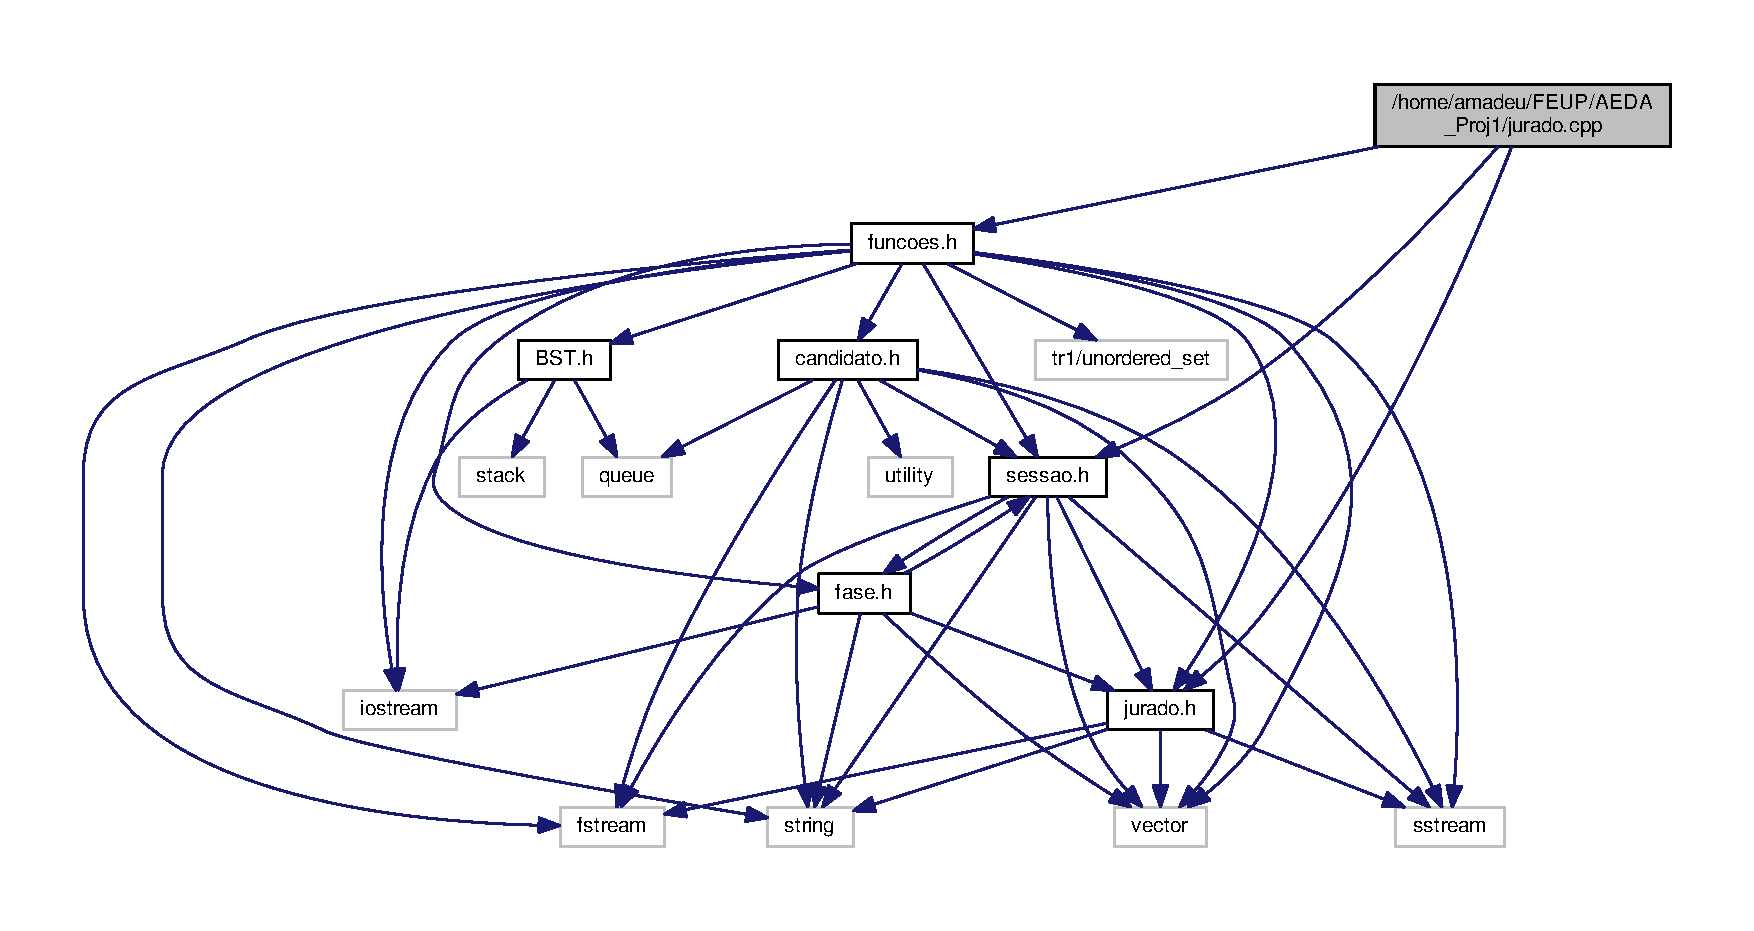
\includegraphics[width=350pt]{jurado_8cpp__incl}
\end{center}
\end{figure}
\subsection*{Functions}
\begin{DoxyCompactItemize}
\item 
std\+::ostream \& \hyperlink{jurado_8cpp_a84fc8870e7ecc1a133a025bf602f2bbb}{operator$<$$<$} (std\+::ostream \&out, const \hyperlink{classJuradoNaoExiste}{Jurado\+Nao\+Existe} \&c)
\item 
std\+::ostream \& \hyperlink{jurado_8cpp_a0b7764f41cc0193d226992c9de898016}{operator$<$$<$} (std\+::ostream \&out, const \hyperlink{classJuradoJaExiste}{Jurado\+Ja\+Existe} \&c)
\item 
std\+::ostream \& \hyperlink{jurado_8cpp_ae3e2a3c64053c2dda11e709db077b1f1}{operator$<$$<$} (std\+::ostream \&out, const \hyperlink{classjuradoOcupado}{jurado\+Ocupado} \&c)
\item 
ostream \& \hyperlink{jurado_8cpp_afbbe037345e49122dbab2fd21278225d}{operator$<$$<$} (ostream \&o, const \hyperlink{classjurado}{jurado} $\ast$j)
\item 
ofstream \& \hyperlink{jurado_8cpp_a9778784aa84765cf798f6cfc59656ce2}{operator$<$$<$} (ofstream \&o, const \hyperlink{classjurado}{jurado} $\ast$j)
\end{DoxyCompactItemize}


\subsection{Function Documentation}
\index{jurado.\+cpp@{jurado.\+cpp}!operator$<$$<$@{operator$<$$<$}}
\index{operator$<$$<$@{operator$<$$<$}!jurado.\+cpp@{jurado.\+cpp}}
\subsubsection[{\texorpdfstring{operator$<$$<$(std\+::ostream \&out, const Jurado\+Nao\+Existe \&c)}{operator<<(std::ostream &out, const JuradoNaoExiste &c)}}]{\setlength{\rightskip}{0pt plus 5cm}std\+::ostream\& operator$<$$<$ (
\begin{DoxyParamCaption}
\item[{std\+::ostream \&}]{out, }
\item[{const {\bf Jurado\+Nao\+Existe} \&}]{c}
\end{DoxyParamCaption}
)}\hypertarget{jurado_8cpp_a84fc8870e7ecc1a133a025bf602f2bbb}{}\label{jurado_8cpp_a84fc8870e7ecc1a133a025bf602f2bbb}
\index{jurado.\+cpp@{jurado.\+cpp}!operator$<$$<$@{operator$<$$<$}}
\index{operator$<$$<$@{operator$<$$<$}!jurado.\+cpp@{jurado.\+cpp}}
\subsubsection[{\texorpdfstring{operator$<$$<$(std\+::ostream \&out, const Jurado\+Ja\+Existe \&c)}{operator<<(std::ostream &out, const JuradoJaExiste &c)}}]{\setlength{\rightskip}{0pt plus 5cm}std\+::ostream\& operator$<$$<$ (
\begin{DoxyParamCaption}
\item[{std\+::ostream \&}]{out, }
\item[{const {\bf Jurado\+Ja\+Existe} \&}]{c}
\end{DoxyParamCaption}
)}\hypertarget{jurado_8cpp_a0b7764f41cc0193d226992c9de898016}{}\label{jurado_8cpp_a0b7764f41cc0193d226992c9de898016}
\index{jurado.\+cpp@{jurado.\+cpp}!operator$<$$<$@{operator$<$$<$}}
\index{operator$<$$<$@{operator$<$$<$}!jurado.\+cpp@{jurado.\+cpp}}
\subsubsection[{\texorpdfstring{operator$<$$<$(std\+::ostream \&out, const jurado\+Ocupado \&c)}{operator<<(std::ostream &out, const juradoOcupado &c)}}]{\setlength{\rightskip}{0pt plus 5cm}std\+::ostream\& operator$<$$<$ (
\begin{DoxyParamCaption}
\item[{std\+::ostream \&}]{out, }
\item[{const {\bf jurado\+Ocupado} \&}]{c}
\end{DoxyParamCaption}
)}\hypertarget{jurado_8cpp_ae3e2a3c64053c2dda11e709db077b1f1}{}\label{jurado_8cpp_ae3e2a3c64053c2dda11e709db077b1f1}
\index{jurado.\+cpp@{jurado.\+cpp}!operator$<$$<$@{operator$<$$<$}}
\index{operator$<$$<$@{operator$<$$<$}!jurado.\+cpp@{jurado.\+cpp}}
\subsubsection[{\texorpdfstring{operator$<$$<$(ostream \&o, const jurado $\ast$j)}{operator<<(ostream &o, const jurado *j)}}]{\setlength{\rightskip}{0pt plus 5cm}ostream\& operator$<$$<$ (
\begin{DoxyParamCaption}
\item[{ostream \&}]{o, }
\item[{const {\bf jurado} $\ast$}]{j}
\end{DoxyParamCaption}
)}\hypertarget{jurado_8cpp_afbbe037345e49122dbab2fd21278225d}{}\label{jurado_8cpp_afbbe037345e49122dbab2fd21278225d}
\index{jurado.\+cpp@{jurado.\+cpp}!operator$<$$<$@{operator$<$$<$}}
\index{operator$<$$<$@{operator$<$$<$}!jurado.\+cpp@{jurado.\+cpp}}
\subsubsection[{\texorpdfstring{operator$<$$<$(ofstream \&o, const jurado $\ast$j)}{operator<<(ofstream &o, const jurado *j)}}]{\setlength{\rightskip}{0pt plus 5cm}ofstream\& operator$<$$<$ (
\begin{DoxyParamCaption}
\item[{ofstream \&}]{o, }
\item[{const {\bf jurado} $\ast$}]{j}
\end{DoxyParamCaption}
)}\hypertarget{jurado_8cpp_a9778784aa84765cf798f6cfc59656ce2}{}\label{jurado_8cpp_a9778784aa84765cf798f6cfc59656ce2}

\hypertarget{jurado_8h}{}\section{/home/amadeu/\+F\+E\+U\+P/\+A\+E\+D\+A\+\_\+\+Proj1/jurado.h File Reference}
\label{jurado_8h}\index{/home/amadeu/\+F\+E\+U\+P/\+A\+E\+D\+A\+\_\+\+Proj1/jurado.\+h@{/home/amadeu/\+F\+E\+U\+P/\+A\+E\+D\+A\+\_\+\+Proj1/jurado.\+h}}
{\ttfamily \#include $<$string$>$}\\*
{\ttfamily \#include $<$vector$>$}\\*
{\ttfamily \#include $<$sstream$>$}\\*
{\ttfamily \#include $<$fstream$>$}\\*
Include dependency graph for jurado.\+h\+:
\nopagebreak
\begin{figure}[H]
\begin{center}
\leavevmode
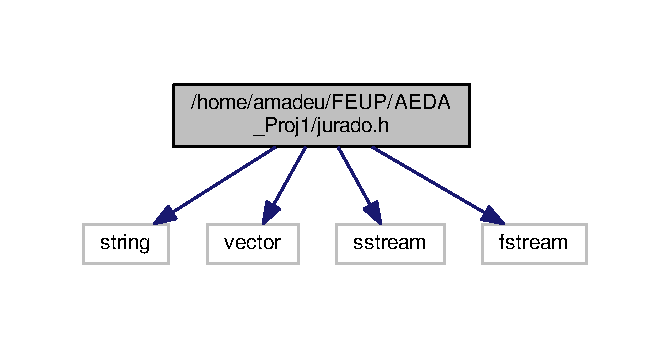
\includegraphics[width=322pt]{jurado_8h__incl}
\end{center}
\end{figure}
This graph shows which files directly or indirectly include this file\+:
\nopagebreak
\begin{figure}[H]
\begin{center}
\leavevmode
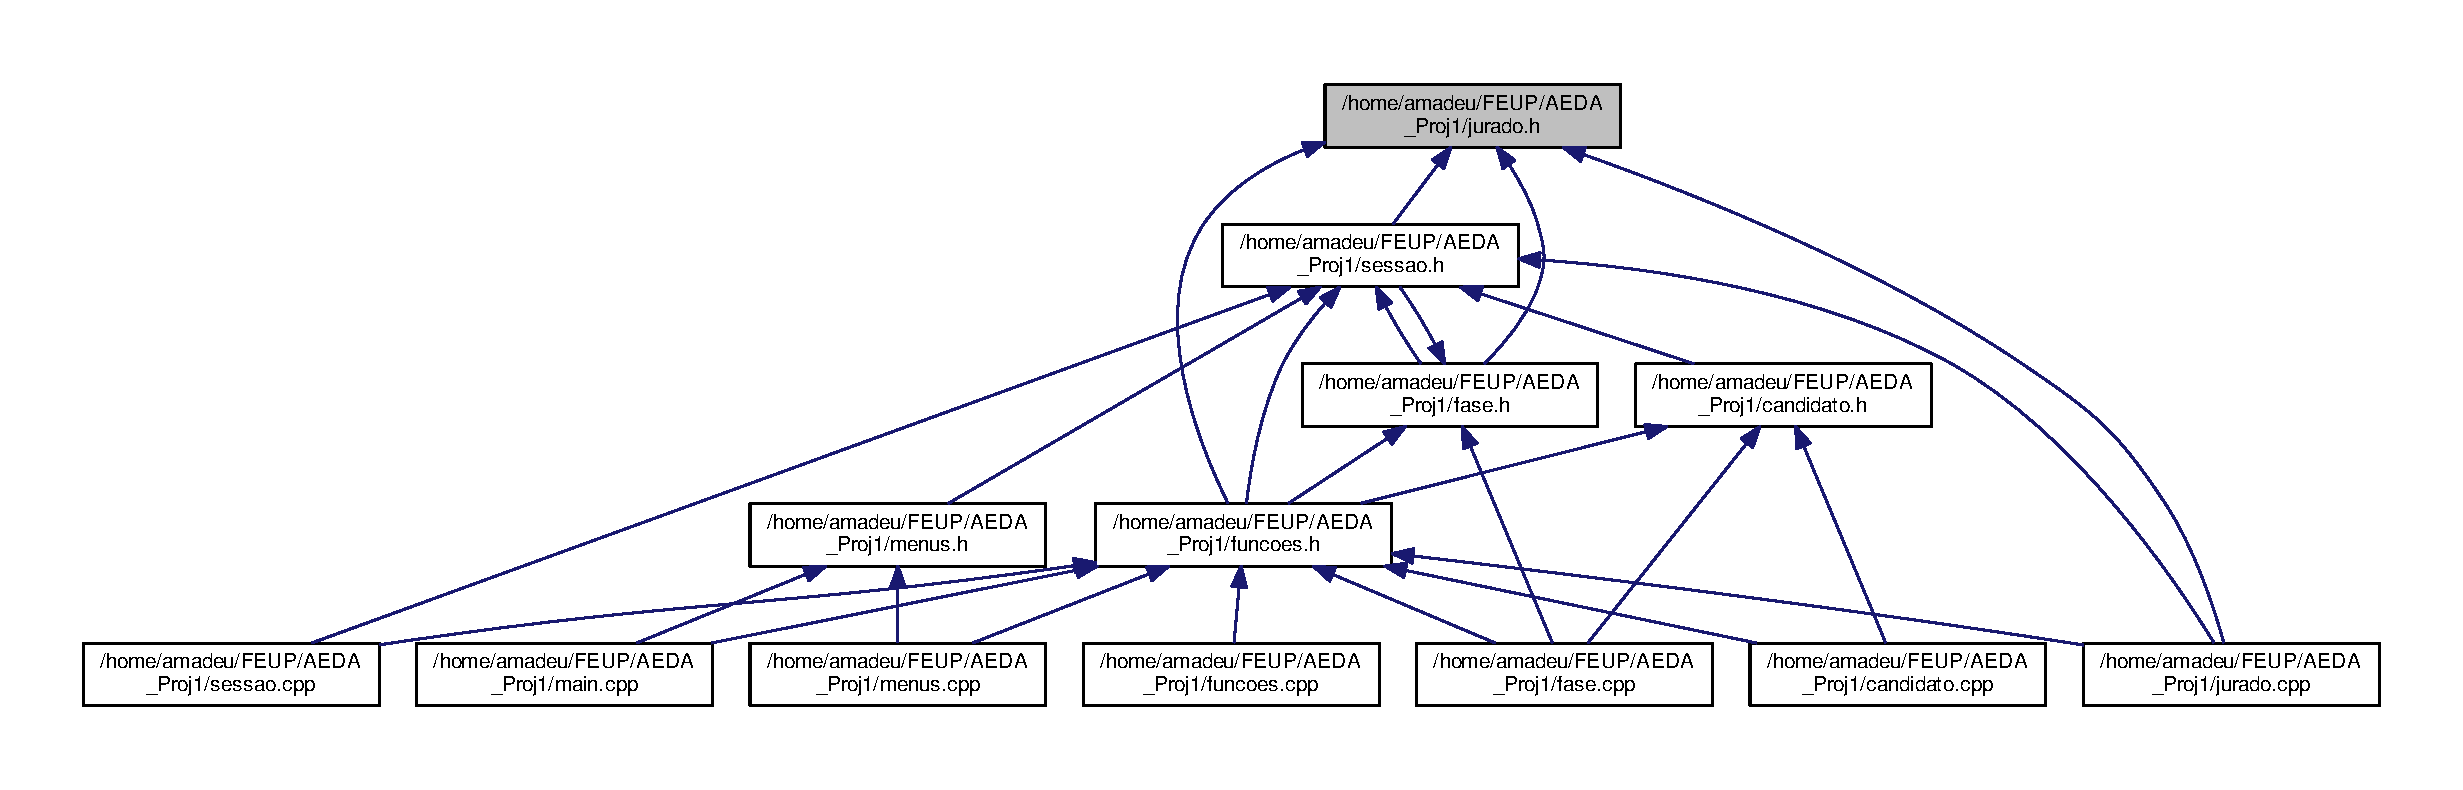
\includegraphics[width=350pt]{jurado_8h__dep__incl}
\end{center}
\end{figure}
\subsection*{Classes}
\begin{DoxyCompactItemize}
\item 
class \hyperlink{classjurado}{jurado}
\begin{DoxyCompactList}\small\item\em classe com as informacoes relativas a um jurado \end{DoxyCompactList}\item 
class \hyperlink{classJuradoNaoExiste}{Jurado\+Nao\+Existe}
\begin{DoxyCompactList}\small\item\em excepcao para quando um objeto da classe jurado nao existe \end{DoxyCompactList}\item 
class \hyperlink{classJuradoJaExiste}{Jurado\+Ja\+Existe}
\begin{DoxyCompactList}\small\item\em excepcao para quando um objeto da classe jurado ja existe \end{DoxyCompactList}\item 
class \hyperlink{classjuradoOcupado}{jurado\+Ocupado}
\begin{DoxyCompactList}\small\item\em excepcao para quando um objeto da classe jurado ja se encontra ocupado num determinado dia \end{DoxyCompactList}\end{DoxyCompactItemize}
\subsection*{Functions}
\begin{DoxyCompactItemize}
\item 
std\+::ostream \& \hyperlink{jurado_8h_a84fc8870e7ecc1a133a025bf602f2bbb}{operator$<$$<$} (std\+::ostream \&out, const \hyperlink{classJuradoNaoExiste}{Jurado\+Nao\+Existe} \&c)
\item 
std\+::ostream \& \hyperlink{jurado_8h_a0b7764f41cc0193d226992c9de898016}{operator$<$$<$} (std\+::ostream \&out, const \hyperlink{classJuradoJaExiste}{Jurado\+Ja\+Existe} \&c)
\item 
std\+::ostream \& \hyperlink{jurado_8h_ae3e2a3c64053c2dda11e709db077b1f1}{operator$<$$<$} (std\+::ostream \&out, const \hyperlink{classjuradoOcupado}{jurado\+Ocupado} \&c)
\end{DoxyCompactItemize}


\subsection{Function Documentation}
\index{jurado.\+h@{jurado.\+h}!operator$<$$<$@{operator$<$$<$}}
\index{operator$<$$<$@{operator$<$$<$}!jurado.\+h@{jurado.\+h}}
\subsubsection[{\texorpdfstring{operator$<$$<$(std\+::ostream \&out, const Jurado\+Nao\+Existe \&c)}{operator<<(std::ostream &out, const JuradoNaoExiste &c)}}]{\setlength{\rightskip}{0pt plus 5cm}std\+::ostream\& operator$<$$<$ (
\begin{DoxyParamCaption}
\item[{std\+::ostream \&}]{out, }
\item[{const {\bf Jurado\+Nao\+Existe} \&}]{c}
\end{DoxyParamCaption}
)}\hypertarget{jurado_8h_a84fc8870e7ecc1a133a025bf602f2bbb}{}\label{jurado_8h_a84fc8870e7ecc1a133a025bf602f2bbb}
\index{jurado.\+h@{jurado.\+h}!operator$<$$<$@{operator$<$$<$}}
\index{operator$<$$<$@{operator$<$$<$}!jurado.\+h@{jurado.\+h}}
\subsubsection[{\texorpdfstring{operator$<$$<$(std\+::ostream \&out, const Jurado\+Ja\+Existe \&c)}{operator<<(std::ostream &out, const JuradoJaExiste &c)}}]{\setlength{\rightskip}{0pt plus 5cm}std\+::ostream\& operator$<$$<$ (
\begin{DoxyParamCaption}
\item[{std\+::ostream \&}]{out, }
\item[{const {\bf Jurado\+Ja\+Existe} \&}]{c}
\end{DoxyParamCaption}
)}\hypertarget{jurado_8h_a0b7764f41cc0193d226992c9de898016}{}\label{jurado_8h_a0b7764f41cc0193d226992c9de898016}
\index{jurado.\+h@{jurado.\+h}!operator$<$$<$@{operator$<$$<$}}
\index{operator$<$$<$@{operator$<$$<$}!jurado.\+h@{jurado.\+h}}
\subsubsection[{\texorpdfstring{operator$<$$<$(std\+::ostream \&out, const jurado\+Ocupado \&c)}{operator<<(std::ostream &out, const juradoOcupado &c)}}]{\setlength{\rightskip}{0pt plus 5cm}std\+::ostream\& operator$<$$<$ (
\begin{DoxyParamCaption}
\item[{std\+::ostream \&}]{out, }
\item[{const {\bf jurado\+Ocupado} \&}]{c}
\end{DoxyParamCaption}
)}\hypertarget{jurado_8h_ae3e2a3c64053c2dda11e709db077b1f1}{}\label{jurado_8h_ae3e2a3c64053c2dda11e709db077b1f1}

\hypertarget{jurados_8txt}{}\section{/home/amadeu/\+F\+E\+U\+P/\+A\+E\+D\+A\+\_\+\+Proj1/jurados.txt File Reference}
\label{jurados_8txt}\index{/home/amadeu/\+F\+E\+U\+P/\+A\+E\+D\+A\+\_\+\+Proj1/jurados.\+txt@{/home/amadeu/\+F\+E\+U\+P/\+A\+E\+D\+A\+\_\+\+Proj1/jurados.\+txt}}
\subsection*{Variables}
\begin{DoxyCompactItemize}
\item 
\hyperlink{jurados_8txt_afae26757e6180cef120017b01ac06140}{Rui}
\item 
\hyperlink{jurados_8txt_a50f37943ca5db274938bcee517a283cc}{porto}
\item 
\hyperlink{sessoes_8txt_a7649ba4017592bd762abe5b976e6481e}{dancar} \hyperlink{jurados_8txt_a3df76ea828422a61d89bb908cc76c7e0}{Raquel}
\item 
\hyperlink{sessoes_8txt_a7649ba4017592bd762abe5b976e6481e}{dancar} \hyperlink{jurados_8txt_afcb0be523bb30dc71d43c136869e3683}{lisboa}
\item 
\hyperlink{sessoes_8txt_a7649ba4017592bd762abe5b976e6481e}{dancar} \hyperlink{sessoes_8txt_a7649ba4017592bd762abe5b976e6481e}{dancar} \hyperlink{jurados_8txt_acaa9f92805c68fb12566e1910b1f38cc}{Marta}
\item 
\hyperlink{sessoes_8txt_a7649ba4017592bd762abe5b976e6481e}{dancar} \hyperlink{sessoes_8txt_a7649ba4017592bd762abe5b976e6481e}{dancar} \hyperlink{jurados_8txt_acb9307bae8c337dfbd877babfe36f1ad}{braga}
\item 
\hyperlink{sessoes_8txt_a7649ba4017592bd762abe5b976e6481e}{dancar} \hyperlink{sessoes_8txt_a7649ba4017592bd762abe5b976e6481e}{dancar} \hyperlink{sessoes_8txt_a2616159a76d0e8a5493734758ae9c160}{cantar} \hyperlink{jurados_8txt_af78ef3d9a9c21ea40fb35f0daf236401}{Pedro}
\item 
\hyperlink{sessoes_8txt_a7649ba4017592bd762abe5b976e6481e}{dancar} \hyperlink{sessoes_8txt_a7649ba4017592bd762abe5b976e6481e}{dancar} \hyperlink{sessoes_8txt_a2616159a76d0e8a5493734758ae9c160}{cantar} \hyperlink{sessoes_8txt_a2616159a76d0e8a5493734758ae9c160}{cantar} \hyperlink{jurados_8txt_ab580858c63900240ff0ab5fcc967078b}{Jose}
\item 
\hyperlink{sessoes_8txt_a7649ba4017592bd762abe5b976e6481e}{dancar} \hyperlink{sessoes_8txt_a7649ba4017592bd762abe5b976e6481e}{dancar} \hyperlink{sessoes_8txt_a2616159a76d0e8a5493734758ae9c160}{cantar} \hyperlink{sessoes_8txt_a2616159a76d0e8a5493734758ae9c160}{cantar} \hyperlink{sessoes_8txt_adb78776c95ad5bfba2eb9fce119157de}{magia} \hyperlink{jurados_8txt_a0b2ef1b8d2f47dfcb6f1424b0fd423be}{Maria}
\item 
\hyperlink{sessoes_8txt_a7649ba4017592bd762abe5b976e6481e}{dancar} \hyperlink{sessoes_8txt_a7649ba4017592bd762abe5b976e6481e}{dancar} \hyperlink{sessoes_8txt_a2616159a76d0e8a5493734758ae9c160}{cantar} \hyperlink{sessoes_8txt_a2616159a76d0e8a5493734758ae9c160}{cantar} \hyperlink{sessoes_8txt_adb78776c95ad5bfba2eb9fce119157de}{magia} vila \hyperlink{jurados_8txt_a793d0656b1424f0c6a8d185ee27b769e}{real}
\item 
\hyperlink{sessoes_8txt_a7649ba4017592bd762abe5b976e6481e}{dancar} \hyperlink{sessoes_8txt_a7649ba4017592bd762abe5b976e6481e}{dancar} \hyperlink{sessoes_8txt_a2616159a76d0e8a5493734758ae9c160}{cantar} \hyperlink{sessoes_8txt_a2616159a76d0e8a5493734758ae9c160}{cantar} \hyperlink{sessoes_8txt_adb78776c95ad5bfba2eb9fce119157de}{magia} vila \hyperlink{sessoes_8txt_a7649ba4017592bd762abe5b976e6481e}{dancar} \hyperlink{jurados_8txt_ad6d47735fc544be4139037eb78a70b69}{Bruno}
\item 
\hyperlink{sessoes_8txt_a7649ba4017592bd762abe5b976e6481e}{dancar} \hyperlink{sessoes_8txt_a7649ba4017592bd762abe5b976e6481e}{dancar} \hyperlink{sessoes_8txt_a2616159a76d0e8a5493734758ae9c160}{cantar} \hyperlink{sessoes_8txt_a2616159a76d0e8a5493734758ae9c160}{cantar} \hyperlink{sessoes_8txt_adb78776c95ad5bfba2eb9fce119157de}{magia} vila \hyperlink{sessoes_8txt_a7649ba4017592bd762abe5b976e6481e}{dancar} \hyperlink{jurados_8txt_a039cea9e32d50e312178ae96d1d2b0b4}{viseu}
\item 
\hyperlink{sessoes_8txt_a7649ba4017592bd762abe5b976e6481e}{dancar} \hyperlink{sessoes_8txt_a7649ba4017592bd762abe5b976e6481e}{dancar} \hyperlink{sessoes_8txt_a2616159a76d0e8a5493734758ae9c160}{cantar} \hyperlink{sessoes_8txt_a2616159a76d0e8a5493734758ae9c160}{cantar} \hyperlink{sessoes_8txt_adb78776c95ad5bfba2eb9fce119157de}{magia} vila \hyperlink{sessoes_8txt_a7649ba4017592bd762abe5b976e6481e}{dancar} \hyperlink{sessoes_8txt_a7649ba4017592bd762abe5b976e6481e}{dancar} \hyperlink{sessoes_8txt_a2616159a76d0e8a5493734758ae9c160}{cantar} \hyperlink{jurados_8txt_a3b70027cdf723e9f232ef7e0a90245e7}{Mario}
\item 
\hyperlink{sessoes_8txt_a7649ba4017592bd762abe5b976e6481e}{dancar} \hyperlink{sessoes_8txt_a7649ba4017592bd762abe5b976e6481e}{dancar} \hyperlink{sessoes_8txt_a2616159a76d0e8a5493734758ae9c160}{cantar} \hyperlink{sessoes_8txt_a2616159a76d0e8a5493734758ae9c160}{cantar} \hyperlink{sessoes_8txt_adb78776c95ad5bfba2eb9fce119157de}{magia} vila \hyperlink{sessoes_8txt_a7649ba4017592bd762abe5b976e6481e}{dancar} \hyperlink{sessoes_8txt_a7649ba4017592bd762abe5b976e6481e}{dancar} \hyperlink{sessoes_8txt_a2616159a76d0e8a5493734758ae9c160}{cantar} \hyperlink{sessoes_8txt_a2616159a76d0e8a5493734758ae9c160}{cantar} \hyperlink{jurados_8txt_a75c689fe94e8e128c28b3115dcb1c08e}{Alexandra}
\item 
\hyperlink{sessoes_8txt_a7649ba4017592bd762abe5b976e6481e}{dancar} \hyperlink{sessoes_8txt_a7649ba4017592bd762abe5b976e6481e}{dancar} \hyperlink{sessoes_8txt_a2616159a76d0e8a5493734758ae9c160}{cantar} \hyperlink{sessoes_8txt_a2616159a76d0e8a5493734758ae9c160}{cantar} \hyperlink{sessoes_8txt_adb78776c95ad5bfba2eb9fce119157de}{magia} vila \hyperlink{sessoes_8txt_a7649ba4017592bd762abe5b976e6481e}{dancar} \hyperlink{sessoes_8txt_a7649ba4017592bd762abe5b976e6481e}{dancar} \hyperlink{sessoes_8txt_a2616159a76d0e8a5493734758ae9c160}{cantar} \hyperlink{sessoes_8txt_a2616159a76d0e8a5493734758ae9c160}{cantar} \hyperlink{jurados_8txt_a7ecd39aca4790a6fae219c51626ebb43}{coimbra}
\item 
\hyperlink{sessoes_8txt_a7649ba4017592bd762abe5b976e6481e}{dancar} \hyperlink{sessoes_8txt_a7649ba4017592bd762abe5b976e6481e}{dancar} \hyperlink{sessoes_8txt_a2616159a76d0e8a5493734758ae9c160}{cantar} \hyperlink{sessoes_8txt_a2616159a76d0e8a5493734758ae9c160}{cantar} \hyperlink{sessoes_8txt_adb78776c95ad5bfba2eb9fce119157de}{magia} vila \hyperlink{sessoes_8txt_a7649ba4017592bd762abe5b976e6481e}{dancar} \hyperlink{sessoes_8txt_a7649ba4017592bd762abe5b976e6481e}{dancar} \hyperlink{sessoes_8txt_a2616159a76d0e8a5493734758ae9c160}{cantar} \hyperlink{sessoes_8txt_a2616159a76d0e8a5493734758ae9c160}{cantar} \hyperlink{sessoes_8txt_adb78776c95ad5bfba2eb9fce119157de}{magia} \hyperlink{jurados_8txt_a5de05656aa2c1e4f1d006ab2c91402f2}{Tiago}
\item 
\hyperlink{sessoes_8txt_a7649ba4017592bd762abe5b976e6481e}{dancar} \hyperlink{sessoes_8txt_a7649ba4017592bd762abe5b976e6481e}{dancar} \hyperlink{sessoes_8txt_a2616159a76d0e8a5493734758ae9c160}{cantar} \hyperlink{sessoes_8txt_a2616159a76d0e8a5493734758ae9c160}{cantar} \hyperlink{sessoes_8txt_adb78776c95ad5bfba2eb9fce119157de}{magia} vila \hyperlink{sessoes_8txt_a7649ba4017592bd762abe5b976e6481e}{dancar} \hyperlink{sessoes_8txt_a7649ba4017592bd762abe5b976e6481e}{dancar} \hyperlink{sessoes_8txt_a2616159a76d0e8a5493734758ae9c160}{cantar} \hyperlink{sessoes_8txt_a2616159a76d0e8a5493734758ae9c160}{cantar} \hyperlink{sessoes_8txt_adb78776c95ad5bfba2eb9fce119157de}{magia} \hyperlink{sessoes_8txt_a7649ba4017592bd762abe5b976e6481e}{dancar} \hyperlink{jurados_8txt_a909a3248ac75b977eaa39caef5735a73}{Miguel}
\end{DoxyCompactItemize}


\subsection{Variable Documentation}
\index{jurados.\+txt@{jurados.\+txt}!Alexandra@{Alexandra}}
\index{Alexandra@{Alexandra}!jurados.\+txt@{jurados.\+txt}}
\subsubsection[{\texorpdfstring{Alexandra}{Alexandra}}]{\setlength{\rightskip}{0pt plus 5cm}{\bf dancar} {\bf dancar} {\bf cantar} {\bf cantar} {\bf magia} vila {\bf dancar} {\bf dancar} {\bf cantar} {\bf cantar} Alexandra}\hypertarget{jurados_8txt_a75c689fe94e8e128c28b3115dcb1c08e}{}\label{jurados_8txt_a75c689fe94e8e128c28b3115dcb1c08e}
\index{jurados.\+txt@{jurados.\+txt}!braga@{braga}}
\index{braga@{braga}!jurados.\+txt@{jurados.\+txt}}
\subsubsection[{\texorpdfstring{braga}{braga}}]{\setlength{\rightskip}{0pt plus 5cm}{\bf dancar} {\bf dancar} {\bf cantar} braga}\hypertarget{jurados_8txt_acb9307bae8c337dfbd877babfe36f1ad}{}\label{jurados_8txt_acb9307bae8c337dfbd877babfe36f1ad}
\index{jurados.\+txt@{jurados.\+txt}!Bruno@{Bruno}}
\index{Bruno@{Bruno}!jurados.\+txt@{jurados.\+txt}}
\subsubsection[{\texorpdfstring{Bruno}{Bruno}}]{\setlength{\rightskip}{0pt plus 5cm}{\bf dancar} {\bf dancar} {\bf cantar} {\bf cantar} {\bf magia} vila {\bf dancar} Bruno}\hypertarget{jurados_8txt_ad6d47735fc544be4139037eb78a70b69}{}\label{jurados_8txt_ad6d47735fc544be4139037eb78a70b69}
\index{jurados.\+txt@{jurados.\+txt}!coimbra@{coimbra}}
\index{coimbra@{coimbra}!jurados.\+txt@{jurados.\+txt}}
\subsubsection[{\texorpdfstring{coimbra}{coimbra}}]{\setlength{\rightskip}{0pt plus 5cm}{\bf dancar} {\bf dancar} {\bf cantar} {\bf cantar} {\bf magia} vila {\bf dancar} {\bf dancar} {\bf cantar} {\bf cantar} {\bf magia} {\bf dancar} coimbra}\hypertarget{jurados_8txt_a7ecd39aca4790a6fae219c51626ebb43}{}\label{jurados_8txt_a7ecd39aca4790a6fae219c51626ebb43}
\index{jurados.\+txt@{jurados.\+txt}!Jose@{Jose}}
\index{Jose@{Jose}!jurados.\+txt@{jurados.\+txt}}
\subsubsection[{\texorpdfstring{Jose}{Jose}}]{\setlength{\rightskip}{0pt plus 5cm}{\bf dancar} {\bf dancar} {\bf cantar} {\bf cantar} Jose}\hypertarget{jurados_8txt_ab580858c63900240ff0ab5fcc967078b}{}\label{jurados_8txt_ab580858c63900240ff0ab5fcc967078b}
\index{jurados.\+txt@{jurados.\+txt}!lisboa@{lisboa}}
\index{lisboa@{lisboa}!jurados.\+txt@{jurados.\+txt}}
\subsubsection[{\texorpdfstring{lisboa}{lisboa}}]{\setlength{\rightskip}{0pt plus 5cm}{\bf dancar} {\bf dancar} {\bf cantar} {\bf cantar} {\bf magia} vila {\bf dancar} {\bf dancar} {\bf cantar} {\bf cantar} {\bf magia} lisboa}\hypertarget{jurados_8txt_afcb0be523bb30dc71d43c136869e3683}{}\label{jurados_8txt_afcb0be523bb30dc71d43c136869e3683}
\index{jurados.\+txt@{jurados.\+txt}!Maria@{Maria}}
\index{Maria@{Maria}!jurados.\+txt@{jurados.\+txt}}
\subsubsection[{\texorpdfstring{Maria}{Maria}}]{\setlength{\rightskip}{0pt plus 5cm}{\bf dancar} {\bf dancar} {\bf cantar} {\bf cantar} {\bf magia} Maria}\hypertarget{jurados_8txt_a0b2ef1b8d2f47dfcb6f1424b0fd423be}{}\label{jurados_8txt_a0b2ef1b8d2f47dfcb6f1424b0fd423be}
\index{jurados.\+txt@{jurados.\+txt}!Mario@{Mario}}
\index{Mario@{Mario}!jurados.\+txt@{jurados.\+txt}}
\subsubsection[{\texorpdfstring{Mario}{Mario}}]{\setlength{\rightskip}{0pt plus 5cm}{\bf dancar} {\bf dancar} {\bf cantar} {\bf cantar} {\bf magia} vila {\bf dancar} {\bf dancar} {\bf cantar} Mario}\hypertarget{jurados_8txt_a3b70027cdf723e9f232ef7e0a90245e7}{}\label{jurados_8txt_a3b70027cdf723e9f232ef7e0a90245e7}
\index{jurados.\+txt@{jurados.\+txt}!Marta@{Marta}}
\index{Marta@{Marta}!jurados.\+txt@{jurados.\+txt}}
\subsubsection[{\texorpdfstring{Marta}{Marta}}]{\setlength{\rightskip}{0pt plus 5cm}{\bf dancar} {\bf dancar} Marta}\hypertarget{jurados_8txt_acaa9f92805c68fb12566e1910b1f38cc}{}\label{jurados_8txt_acaa9f92805c68fb12566e1910b1f38cc}
\index{jurados.\+txt@{jurados.\+txt}!Miguel@{Miguel}}
\index{Miguel@{Miguel}!jurados.\+txt@{jurados.\+txt}}
\subsubsection[{\texorpdfstring{Miguel}{Miguel}}]{\setlength{\rightskip}{0pt plus 5cm}{\bf dancar} {\bf dancar} {\bf cantar} {\bf cantar} {\bf magia} vila {\bf dancar} {\bf dancar} {\bf cantar} {\bf cantar} {\bf magia} {\bf dancar} Miguel}\hypertarget{jurados_8txt_a909a3248ac75b977eaa39caef5735a73}{}\label{jurados_8txt_a909a3248ac75b977eaa39caef5735a73}
\index{jurados.\+txt@{jurados.\+txt}!Pedro@{Pedro}}
\index{Pedro@{Pedro}!jurados.\+txt@{jurados.\+txt}}
\subsubsection[{\texorpdfstring{Pedro}{Pedro}}]{\setlength{\rightskip}{0pt plus 5cm}{\bf dancar} {\bf dancar} {\bf cantar} Pedro}\hypertarget{jurados_8txt_af78ef3d9a9c21ea40fb35f0daf236401}{}\label{jurados_8txt_af78ef3d9a9c21ea40fb35f0daf236401}
\index{jurados.\+txt@{jurados.\+txt}!porto@{porto}}
\index{porto@{porto}!jurados.\+txt@{jurados.\+txt}}
\subsubsection[{\texorpdfstring{porto}{porto}}]{\setlength{\rightskip}{0pt plus 5cm}{\bf dancar} {\bf dancar} {\bf cantar} {\bf cantar} {\bf magia} vila {\bf dancar} {\bf dancar} {\bf cantar} porto}\hypertarget{jurados_8txt_a50f37943ca5db274938bcee517a283cc}{}\label{jurados_8txt_a50f37943ca5db274938bcee517a283cc}
\index{jurados.\+txt@{jurados.\+txt}!Raquel@{Raquel}}
\index{Raquel@{Raquel}!jurados.\+txt@{jurados.\+txt}}
\subsubsection[{\texorpdfstring{Raquel}{Raquel}}]{\setlength{\rightskip}{0pt plus 5cm}{\bf dancar} Raquel}\hypertarget{jurados_8txt_a3df76ea828422a61d89bb908cc76c7e0}{}\label{jurados_8txt_a3df76ea828422a61d89bb908cc76c7e0}
\index{jurados.\+txt@{jurados.\+txt}!real@{real}}
\index{real@{real}!jurados.\+txt@{jurados.\+txt}}
\subsubsection[{\texorpdfstring{real}{real}}]{\setlength{\rightskip}{0pt plus 5cm}{\bf dancar} {\bf dancar} {\bf cantar} {\bf cantar} {\bf magia} vila real}\hypertarget{jurados_8txt_a793d0656b1424f0c6a8d185ee27b769e}{}\label{jurados_8txt_a793d0656b1424f0c6a8d185ee27b769e}
\index{jurados.\+txt@{jurados.\+txt}!Rui@{Rui}}
\index{Rui@{Rui}!jurados.\+txt@{jurados.\+txt}}
\subsubsection[{\texorpdfstring{Rui}{Rui}}]{\setlength{\rightskip}{0pt plus 5cm}{\bf dancar} {\bf dancar} {\bf cantar} {\bf cantar} {\bf magia} vila {\bf dancar} {\bf dancar} Rui}\hypertarget{jurados_8txt_afae26757e6180cef120017b01ac06140}{}\label{jurados_8txt_afae26757e6180cef120017b01ac06140}
\index{jurados.\+txt@{jurados.\+txt}!Tiago@{Tiago}}
\index{Tiago@{Tiago}!jurados.\+txt@{jurados.\+txt}}
\subsubsection[{\texorpdfstring{Tiago}{Tiago}}]{\setlength{\rightskip}{0pt plus 5cm}{\bf dancar} {\bf dancar} {\bf cantar} {\bf cantar} {\bf magia} vila {\bf dancar} {\bf dancar} {\bf cantar} {\bf cantar} {\bf magia} Tiago}\hypertarget{jurados_8txt_a5de05656aa2c1e4f1d006ab2c91402f2}{}\label{jurados_8txt_a5de05656aa2c1e4f1d006ab2c91402f2}
\index{jurados.\+txt@{jurados.\+txt}!viseu@{viseu}}
\index{viseu@{viseu}!jurados.\+txt@{jurados.\+txt}}
\subsubsection[{\texorpdfstring{viseu}{viseu}}]{\setlength{\rightskip}{0pt plus 5cm}{\bf dancar} {\bf dancar} {\bf cantar} {\bf cantar} {\bf magia} vila {\bf dancar} {\bf dancar} viseu}\hypertarget{jurados_8txt_a039cea9e32d50e312178ae96d1d2b0b4}{}\label{jurados_8txt_a039cea9e32d50e312178ae96d1d2b0b4}

\hypertarget{main_8cpp}{}\section{/home/amadeu/\+F\+E\+U\+P/\+A\+E\+D\+A\+\_\+\+Proj1/main.cpp File Reference}
\label{main_8cpp}\index{/home/amadeu/\+F\+E\+U\+P/\+A\+E\+D\+A\+\_\+\+Proj1/main.\+cpp@{/home/amadeu/\+F\+E\+U\+P/\+A\+E\+D\+A\+\_\+\+Proj1/main.\+cpp}}
{\ttfamily \#include \char`\"{}funcoes.\+h\char`\"{}}\\*
{\ttfamily \#include \char`\"{}menus.\+h\char`\"{}}\\*
Include dependency graph for main.\+cpp\+:
\nopagebreak
\begin{figure}[H]
\begin{center}
\leavevmode
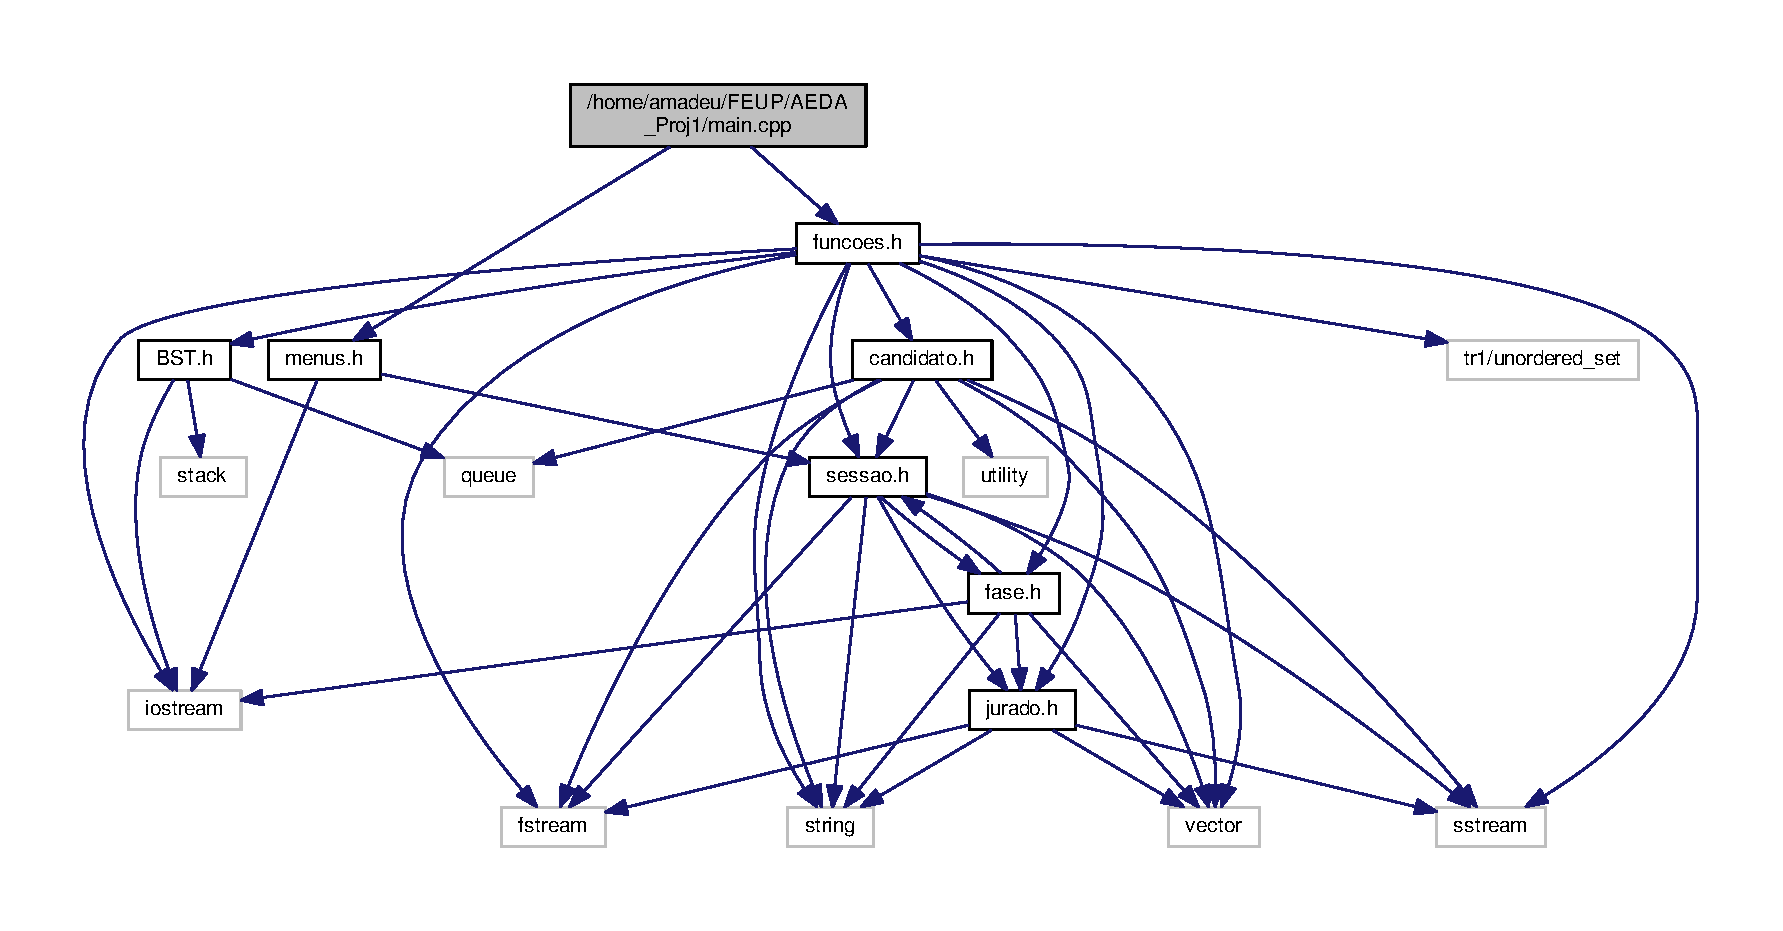
\includegraphics[width=350pt]{main_8cpp__incl}
\end{center}
\end{figure}
\subsection*{Functions}
\begin{DoxyCompactItemize}
\item 
int \hyperlink{main_8cpp_ae66f6b31b5ad750f1fe042a706a4e3d4}{main} ()
\end{DoxyCompactItemize}


\subsection{Function Documentation}
\index{main.\+cpp@{main.\+cpp}!main@{main}}
\index{main@{main}!main.\+cpp@{main.\+cpp}}
\subsubsection[{\texorpdfstring{main()}{main()}}]{\setlength{\rightskip}{0pt plus 5cm}int main (
\begin{DoxyParamCaption}
{}
\end{DoxyParamCaption}
)}\hypertarget{main_8cpp_ae66f6b31b5ad750f1fe042a706a4e3d4}{}\label{main_8cpp_ae66f6b31b5ad750f1fe042a706a4e3d4}

\hypertarget{menus_8cpp}{}\section{/home/amadeu/\+F\+E\+U\+P/\+A\+E\+D\+A\+\_\+\+Proj1/menus.cpp File Reference}
\label{menus_8cpp}\index{/home/amadeu/\+F\+E\+U\+P/\+A\+E\+D\+A\+\_\+\+Proj1/menus.\+cpp@{/home/amadeu/\+F\+E\+U\+P/\+A\+E\+D\+A\+\_\+\+Proj1/menus.\+cpp}}
{\ttfamily \#include $<$utility$>$}\\*
{\ttfamily \#include \char`\"{}menus.\+h\char`\"{}}\\*
{\ttfamily \#include \char`\"{}funcoes.\+h\char`\"{}}\\*
Include dependency graph for menus.\+cpp\+:
\nopagebreak
\begin{figure}[H]
\begin{center}
\leavevmode
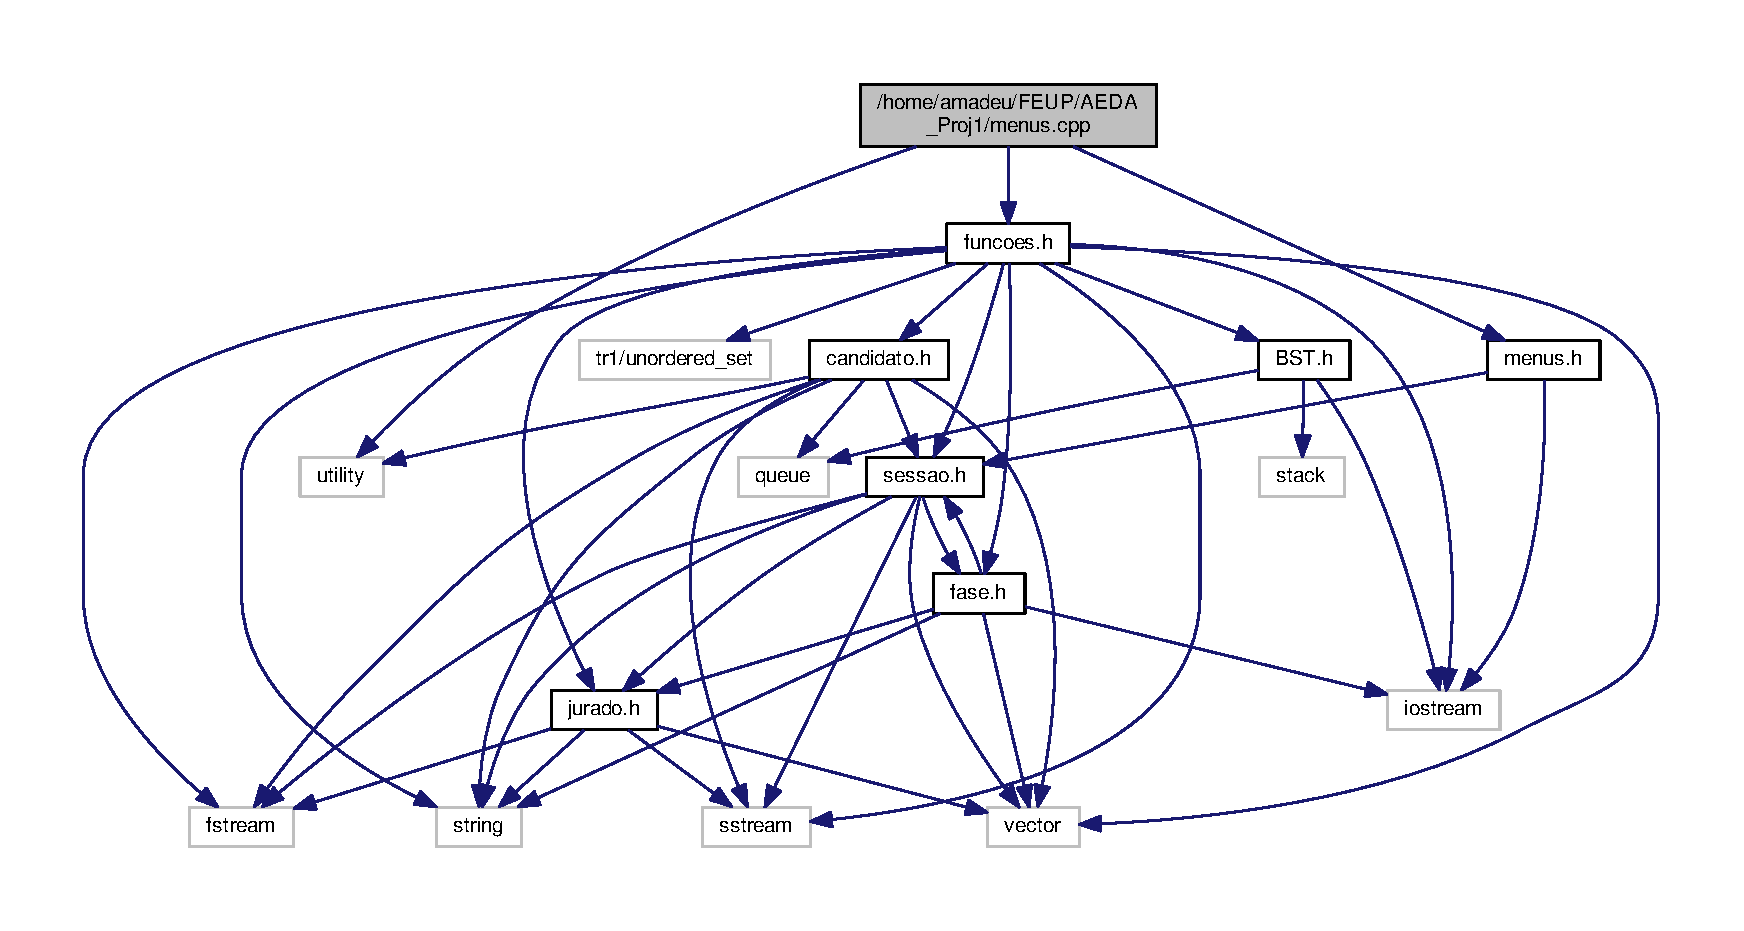
\includegraphics[width=350pt]{menus_8cpp__incl}
\end{center}
\end{figure}
\subsection*{Functions}
\begin{DoxyCompactItemize}
\item 
void \hyperlink{menus_8cpp_a2a0e843767aeea4f433a28b9c54f573a}{menu} ()
\begin{DoxyCompactList}\small\item\em display do menu geral \end{DoxyCompactList}\item 
void \hyperlink{menus_8cpp_aab42b4271b882e2866f715920fcc5cef}{menu\+Candidatos} ()
\begin{DoxyCompactList}\small\item\em display do menu sobre os candidatos \end{DoxyCompactList}\item 
void \hyperlink{menus_8cpp_a9f532c9708d3f1997c55f6953bf652a4}{menu\+Jurados} ()
\begin{DoxyCompactList}\small\item\em display do menu sobre os jurados \end{DoxyCompactList}\item 
void \hyperlink{menus_8cpp_aeee7823bb4eb32e2795658999fde69e1}{menu\+Sessoes} ()
\begin{DoxyCompactList}\small\item\em display do menu acerca das varias sessoes \end{DoxyCompactList}\item 
void \hyperlink{menus_8cpp_a47dfe7486994b86baf402fc6be377475}{menu\+Adiciona\+Candidato} ()
\begin{DoxyCompactList}\small\item\em display do menu para adicionar um candidato \end{DoxyCompactList}\item 
void \hyperlink{menus_8cpp_a400dfb19e4bb59078fa09a4b184d22ef}{menu\+Remove\+Candidato} ()
\begin{DoxyCompactList}\small\item\em display do menu para remover um candidato \end{DoxyCompactList}\item 
void \hyperlink{menus_8cpp_a4ec260bdab29eb9b9637b39ef7dafa81}{menu\+Remove\+Candidato\+Numero} ()
\begin{DoxyCompactList}\small\item\em display do menu para remover um candidato com base no numero \end{DoxyCompactList}\item 
void \hyperlink{menus_8cpp_ad0a26823c8b0f7d0efc28c19c5685654}{menu\+Remove\+Candidato\+Nome} ()
\begin{DoxyCompactList}\small\item\em display do menu para remover um candidato com base no nome \end{DoxyCompactList}\item 
void \hyperlink{menus_8cpp_aea371219232565dc7858716a1bd47817}{menu\+Alterar\+Candidato} ()
\item 
void \hyperlink{menus_8cpp_a11b81ccf581a04e7630e65f8bd1bbbfa}{menu\+Alterar\+Candidato\+Numero} ()
\begin{DoxyCompactList}\small\item\em display do menu para alterar um candidato com base no numero \end{DoxyCompactList}\item 
void \hyperlink{menus_8cpp_aac0a29a50eef36bfd6ac7f627fa5bdec}{menu\+Alterar\+Candidato\+Nome} ()
\begin{DoxyCompactList}\small\item\em display do menu para alterar um candidato com base no nome \end{DoxyCompactList}\item 
void \hyperlink{menus_8cpp_ac2635799f82961fd2b0ec1f422967559}{menu\+Info\+Candidato} ()
\begin{DoxyCompactList}\small\item\em display do menu para ver a informacao dos candidatos \end{DoxyCompactList}\item 
void \hyperlink{menus_8cpp_a185fea948b263fa812288e236b2bd19a}{menu\+Info\+Candidato\+Numero} ()
\begin{DoxyCompactList}\small\item\em display do menu para procurar e ver a informacao de um candidato \end{DoxyCompactList}\item 
void \hyperlink{menus_8cpp_ae726400850a6789056a264558b233109}{menu\+Info\+Candidato\+Todos} ()
\begin{DoxyCompactList}\small\item\em display do menu para ver a informacao de todos os candidatos \end{DoxyCompactList}\item 
void \hyperlink{menus_8cpp_a2e5524ba2150e12fdabb7e0e42b5e940}{menu\+Info\+Candidatos\+Arte} ()
\begin{DoxyCompactList}\small\item\em display de todos os candidatos de uma arte perfomativa \end{DoxyCompactList}\item 
void \hyperlink{menus_8cpp_aa4f9c781fd709e6dff3db8cdbb2e27eb}{menu\+Adiciona\+Jurado} ()
\begin{DoxyCompactList}\small\item\em display do menu para adicionar um jurado \end{DoxyCompactList}\item 
void \hyperlink{menus_8cpp_a8ca47d3453fc44081302fdaac73c29f4}{menu\+Remove\+Jurado} ()
\begin{DoxyCompactList}\small\item\em display do menu para remover um jurado \end{DoxyCompactList}\item 
void \hyperlink{menus_8cpp_a69680649d07e58b0874bedeec5e00287}{menu\+Info\+Jurado} ()
\begin{DoxyCompactList}\small\item\em display do menu para ver a informacao dos candidatos \end{DoxyCompactList}\item 
void \hyperlink{menus_8cpp_ac8df289c83dac877629f7b11ae1f0947}{menu\+Info\+Jurado\+Nome} ()
\begin{DoxyCompactList}\small\item\em display do menu para procurar e ver a informacao de um jurado; \end{DoxyCompactList}\item 
void \hyperlink{menus_8cpp_a7d36bf5ec3b83ddb45a42760966be7b2}{menu\+Info\+Jurado\+Todos} ()
\begin{DoxyCompactList}\small\item\em display do menu para ver a informacao de todos os jurados \end{DoxyCompactList}\item 
void \hyperlink{menus_8cpp_a99f9a7afd9aeeb017fdf54b19fd223ef}{menu\+Adiciona\+Sessao} ()
\begin{DoxyCompactList}\small\item\em display do menu para adicionar uma sessao \end{DoxyCompactList}\item 
void \hyperlink{menus_8cpp_a93fea54aa1e26d7939776646bffc75ec}{menu\+Remove\+Sessao} ()
\begin{DoxyCompactList}\small\item\em display do menu para remover uma sessao \end{DoxyCompactList}\item 
void \hyperlink{menus_8cpp_ad8a0f4f72ff3592f271ceef3eb844185}{menu\+Adiciona\+Candidatos\+Sessao} (\hyperlink{classsessao}{sessao} $\ast$s)
\begin{DoxyCompactList}\small\item\em display do menu para adicionar candidatos a uma sessao \end{DoxyCompactList}\item 
int \hyperlink{menus_8cpp_a8555f02addba03c2b1f3702485995343}{menu\+Adiciona\+Jurados\+Sessao} (\hyperlink{classsessao}{sessao} $\ast$s)
\begin{DoxyCompactList}\small\item\em display do menu para adicionar jurados a uma sessao \end{DoxyCompactList}\item 
void \hyperlink{menus_8cpp_a47bc5591a007353eab848fbaf653447c}{menu\+Info\+Sessoes} ()
\begin{DoxyCompactList}\small\item\em display do menu para obter informacao de uma sessao \end{DoxyCompactList}\item 
void \hyperlink{menus_8cpp_a290c79dfdc80552b575fb89f0793d403}{menu\+Iniciar\+Sessao} ()
\end{DoxyCompactItemize}


\subsection{Function Documentation}
\index{menus.\+cpp@{menus.\+cpp}!menu@{menu}}
\index{menu@{menu}!menus.\+cpp@{menus.\+cpp}}
\subsubsection[{\texorpdfstring{menu()}{menu()}}]{\setlength{\rightskip}{0pt plus 5cm}void menu (
\begin{DoxyParamCaption}
{}
\end{DoxyParamCaption}
)}\hypertarget{menus_8cpp_a2a0e843767aeea4f433a28b9c54f573a}{}\label{menus_8cpp_a2a0e843767aeea4f433a28b9c54f573a}


display do menu geral 

\index{menus.\+cpp@{menus.\+cpp}!menu\+Adiciona\+Candidato@{menu\+Adiciona\+Candidato}}
\index{menu\+Adiciona\+Candidato@{menu\+Adiciona\+Candidato}!menus.\+cpp@{menus.\+cpp}}
\subsubsection[{\texorpdfstring{menu\+Adiciona\+Candidato()}{menuAdicionaCandidato()}}]{\setlength{\rightskip}{0pt plus 5cm}void menu\+Adiciona\+Candidato (
\begin{DoxyParamCaption}
{}
\end{DoxyParamCaption}
)}\hypertarget{menus_8cpp_a47dfe7486994b86baf402fc6be377475}{}\label{menus_8cpp_a47dfe7486994b86baf402fc6be377475}


display do menu para adicionar um candidato 

\index{menus.\+cpp@{menus.\+cpp}!menu\+Adiciona\+Candidatos\+Sessao@{menu\+Adiciona\+Candidatos\+Sessao}}
\index{menu\+Adiciona\+Candidatos\+Sessao@{menu\+Adiciona\+Candidatos\+Sessao}!menus.\+cpp@{menus.\+cpp}}
\subsubsection[{\texorpdfstring{menu\+Adiciona\+Candidatos\+Sessao(sessao $\ast$s)}{menuAdicionaCandidatosSessao(sessao *s)}}]{\setlength{\rightskip}{0pt plus 5cm}void menu\+Adiciona\+Candidatos\+Sessao (
\begin{DoxyParamCaption}
\item[{{\bf sessao} $\ast$}]{s}
\end{DoxyParamCaption}
)}\hypertarget{menus_8cpp_ad8a0f4f72ff3592f271ceef3eb844185}{}\label{menus_8cpp_ad8a0f4f72ff3592f271ceef3eb844185}


display do menu para adicionar candidatos a uma sessao 


\begin{DoxyParams}{Parameters}
{\em s} & sessao a que se pretende adicionar candidatos \\
\hline
\end{DoxyParams}
\index{menus.\+cpp@{menus.\+cpp}!menu\+Adiciona\+Jurado@{menu\+Adiciona\+Jurado}}
\index{menu\+Adiciona\+Jurado@{menu\+Adiciona\+Jurado}!menus.\+cpp@{menus.\+cpp}}
\subsubsection[{\texorpdfstring{menu\+Adiciona\+Jurado()}{menuAdicionaJurado()}}]{\setlength{\rightskip}{0pt plus 5cm}void menu\+Adiciona\+Jurado (
\begin{DoxyParamCaption}
{}
\end{DoxyParamCaption}
)}\hypertarget{menus_8cpp_aa4f9c781fd709e6dff3db8cdbb2e27eb}{}\label{menus_8cpp_aa4f9c781fd709e6dff3db8cdbb2e27eb}


display do menu para adicionar um jurado 

\index{menus.\+cpp@{menus.\+cpp}!menu\+Adiciona\+Jurados\+Sessao@{menu\+Adiciona\+Jurados\+Sessao}}
\index{menu\+Adiciona\+Jurados\+Sessao@{menu\+Adiciona\+Jurados\+Sessao}!menus.\+cpp@{menus.\+cpp}}
\subsubsection[{\texorpdfstring{menu\+Adiciona\+Jurados\+Sessao(sessao $\ast$s)}{menuAdicionaJuradosSessao(sessao *s)}}]{\setlength{\rightskip}{0pt plus 5cm}int menu\+Adiciona\+Jurados\+Sessao (
\begin{DoxyParamCaption}
\item[{{\bf sessao} $\ast$}]{s}
\end{DoxyParamCaption}
)}\hypertarget{menus_8cpp_a8555f02addba03c2b1f3702485995343}{}\label{menus_8cpp_a8555f02addba03c2b1f3702485995343}


display do menu para adicionar jurados a uma sessao 


\begin{DoxyParams}{Parameters}
{\em s} & sessao a que se pretende adicionar jurados \\
\hline
\end{DoxyParams}
\begin{DoxyReturn}{Returns}
devolve 1 se nao existirem jurados suficientes para criar uma sessao 
\end{DoxyReturn}
\index{menus.\+cpp@{menus.\+cpp}!menu\+Adiciona\+Sessao@{menu\+Adiciona\+Sessao}}
\index{menu\+Adiciona\+Sessao@{menu\+Adiciona\+Sessao}!menus.\+cpp@{menus.\+cpp}}
\subsubsection[{\texorpdfstring{menu\+Adiciona\+Sessao()}{menuAdicionaSessao()}}]{\setlength{\rightskip}{0pt plus 5cm}void menu\+Adiciona\+Sessao (
\begin{DoxyParamCaption}
{}
\end{DoxyParamCaption}
)}\hypertarget{menus_8cpp_a99f9a7afd9aeeb017fdf54b19fd223ef}{}\label{menus_8cpp_a99f9a7afd9aeeb017fdf54b19fd223ef}


display do menu para adicionar uma sessao 

\index{menus.\+cpp@{menus.\+cpp}!menu\+Alterar\+Candidato@{menu\+Alterar\+Candidato}}
\index{menu\+Alterar\+Candidato@{menu\+Alterar\+Candidato}!menus.\+cpp@{menus.\+cpp}}
\subsubsection[{\texorpdfstring{menu\+Alterar\+Candidato()}{menuAlterarCandidato()}}]{\setlength{\rightskip}{0pt plus 5cm}void menu\+Alterar\+Candidato (
\begin{DoxyParamCaption}
{}
\end{DoxyParamCaption}
)}\hypertarget{menus_8cpp_aea371219232565dc7858716a1bd47817}{}\label{menus_8cpp_aea371219232565dc7858716a1bd47817}
display do menu para alterar a informacao de um candidato \index{menus.\+cpp@{menus.\+cpp}!menu\+Alterar\+Candidato\+Nome@{menu\+Alterar\+Candidato\+Nome}}
\index{menu\+Alterar\+Candidato\+Nome@{menu\+Alterar\+Candidato\+Nome}!menus.\+cpp@{menus.\+cpp}}
\subsubsection[{\texorpdfstring{menu\+Alterar\+Candidato\+Nome()}{menuAlterarCandidatoNome()}}]{\setlength{\rightskip}{0pt plus 5cm}void menu\+Alterar\+Candidato\+Nome (
\begin{DoxyParamCaption}
{}
\end{DoxyParamCaption}
)}\hypertarget{menus_8cpp_aac0a29a50eef36bfd6ac7f627fa5bdec}{}\label{menus_8cpp_aac0a29a50eef36bfd6ac7f627fa5bdec}


display do menu para alterar um candidato com base no nome 

\index{menus.\+cpp@{menus.\+cpp}!menu\+Alterar\+Candidato\+Numero@{menu\+Alterar\+Candidato\+Numero}}
\index{menu\+Alterar\+Candidato\+Numero@{menu\+Alterar\+Candidato\+Numero}!menus.\+cpp@{menus.\+cpp}}
\subsubsection[{\texorpdfstring{menu\+Alterar\+Candidato\+Numero()}{menuAlterarCandidatoNumero()}}]{\setlength{\rightskip}{0pt plus 5cm}void menu\+Alterar\+Candidato\+Numero (
\begin{DoxyParamCaption}
{}
\end{DoxyParamCaption}
)}\hypertarget{menus_8cpp_a11b81ccf581a04e7630e65f8bd1bbbfa}{}\label{menus_8cpp_a11b81ccf581a04e7630e65f8bd1bbbfa}


display do menu para alterar um candidato com base no numero 

\index{menus.\+cpp@{menus.\+cpp}!menu\+Candidatos@{menu\+Candidatos}}
\index{menu\+Candidatos@{menu\+Candidatos}!menus.\+cpp@{menus.\+cpp}}
\subsubsection[{\texorpdfstring{menu\+Candidatos()}{menuCandidatos()}}]{\setlength{\rightskip}{0pt plus 5cm}void menu\+Candidatos (
\begin{DoxyParamCaption}
{}
\end{DoxyParamCaption}
)}\hypertarget{menus_8cpp_aab42b4271b882e2866f715920fcc5cef}{}\label{menus_8cpp_aab42b4271b882e2866f715920fcc5cef}


display do menu sobre os candidatos 

\index{menus.\+cpp@{menus.\+cpp}!menu\+Info\+Candidato@{menu\+Info\+Candidato}}
\index{menu\+Info\+Candidato@{menu\+Info\+Candidato}!menus.\+cpp@{menus.\+cpp}}
\subsubsection[{\texorpdfstring{menu\+Info\+Candidato()}{menuInfoCandidato()}}]{\setlength{\rightskip}{0pt plus 5cm}void menu\+Info\+Candidato (
\begin{DoxyParamCaption}
{}
\end{DoxyParamCaption}
)}\hypertarget{menus_8cpp_ac2635799f82961fd2b0ec1f422967559}{}\label{menus_8cpp_ac2635799f82961fd2b0ec1f422967559}


display do menu para ver a informacao dos candidatos 

\index{menus.\+cpp@{menus.\+cpp}!menu\+Info\+Candidato\+Numero@{menu\+Info\+Candidato\+Numero}}
\index{menu\+Info\+Candidato\+Numero@{menu\+Info\+Candidato\+Numero}!menus.\+cpp@{menus.\+cpp}}
\subsubsection[{\texorpdfstring{menu\+Info\+Candidato\+Numero()}{menuInfoCandidatoNumero()}}]{\setlength{\rightskip}{0pt plus 5cm}void menu\+Info\+Candidato\+Numero (
\begin{DoxyParamCaption}
{}
\end{DoxyParamCaption}
)}\hypertarget{menus_8cpp_a185fea948b263fa812288e236b2bd19a}{}\label{menus_8cpp_a185fea948b263fa812288e236b2bd19a}


display do menu para procurar e ver a informacao de um candidato 

\index{menus.\+cpp@{menus.\+cpp}!menu\+Info\+Candidatos\+Arte@{menu\+Info\+Candidatos\+Arte}}
\index{menu\+Info\+Candidatos\+Arte@{menu\+Info\+Candidatos\+Arte}!menus.\+cpp@{menus.\+cpp}}
\subsubsection[{\texorpdfstring{menu\+Info\+Candidatos\+Arte()}{menuInfoCandidatosArte()}}]{\setlength{\rightskip}{0pt plus 5cm}void menu\+Info\+Candidatos\+Arte (
\begin{DoxyParamCaption}
{}
\end{DoxyParamCaption}
)}\hypertarget{menus_8cpp_a2e5524ba2150e12fdabb7e0e42b5e940}{}\label{menus_8cpp_a2e5524ba2150e12fdabb7e0e42b5e940}


display de todos os candidatos de uma arte perfomativa 

\index{menus.\+cpp@{menus.\+cpp}!menu\+Info\+Candidato\+Todos@{menu\+Info\+Candidato\+Todos}}
\index{menu\+Info\+Candidato\+Todos@{menu\+Info\+Candidato\+Todos}!menus.\+cpp@{menus.\+cpp}}
\subsubsection[{\texorpdfstring{menu\+Info\+Candidato\+Todos()}{menuInfoCandidatoTodos()}}]{\setlength{\rightskip}{0pt plus 5cm}void menu\+Info\+Candidato\+Todos (
\begin{DoxyParamCaption}
{}
\end{DoxyParamCaption}
)}\hypertarget{menus_8cpp_ae726400850a6789056a264558b233109}{}\label{menus_8cpp_ae726400850a6789056a264558b233109}


display do menu para ver a informacao de todos os candidatos 

\index{menus.\+cpp@{menus.\+cpp}!menu\+Info\+Jurado@{menu\+Info\+Jurado}}
\index{menu\+Info\+Jurado@{menu\+Info\+Jurado}!menus.\+cpp@{menus.\+cpp}}
\subsubsection[{\texorpdfstring{menu\+Info\+Jurado()}{menuInfoJurado()}}]{\setlength{\rightskip}{0pt plus 5cm}void menu\+Info\+Jurado (
\begin{DoxyParamCaption}
{}
\end{DoxyParamCaption}
)}\hypertarget{menus_8cpp_a69680649d07e58b0874bedeec5e00287}{}\label{menus_8cpp_a69680649d07e58b0874bedeec5e00287}


display do menu para ver a informacao dos candidatos 

\index{menus.\+cpp@{menus.\+cpp}!menu\+Info\+Jurado\+Nome@{menu\+Info\+Jurado\+Nome}}
\index{menu\+Info\+Jurado\+Nome@{menu\+Info\+Jurado\+Nome}!menus.\+cpp@{menus.\+cpp}}
\subsubsection[{\texorpdfstring{menu\+Info\+Jurado\+Nome()}{menuInfoJuradoNome()}}]{\setlength{\rightskip}{0pt plus 5cm}void menu\+Info\+Jurado\+Nome (
\begin{DoxyParamCaption}
{}
\end{DoxyParamCaption}
)}\hypertarget{menus_8cpp_ac8df289c83dac877629f7b11ae1f0947}{}\label{menus_8cpp_ac8df289c83dac877629f7b11ae1f0947}


display do menu para procurar e ver a informacao de um jurado; 

\index{menus.\+cpp@{menus.\+cpp}!menu\+Info\+Jurado\+Todos@{menu\+Info\+Jurado\+Todos}}
\index{menu\+Info\+Jurado\+Todos@{menu\+Info\+Jurado\+Todos}!menus.\+cpp@{menus.\+cpp}}
\subsubsection[{\texorpdfstring{menu\+Info\+Jurado\+Todos()}{menuInfoJuradoTodos()}}]{\setlength{\rightskip}{0pt plus 5cm}void menu\+Info\+Jurado\+Todos (
\begin{DoxyParamCaption}
{}
\end{DoxyParamCaption}
)}\hypertarget{menus_8cpp_a7d36bf5ec3b83ddb45a42760966be7b2}{}\label{menus_8cpp_a7d36bf5ec3b83ddb45a42760966be7b2}


display do menu para ver a informacao de todos os jurados 

\index{menus.\+cpp@{menus.\+cpp}!menu\+Info\+Sessoes@{menu\+Info\+Sessoes}}
\index{menu\+Info\+Sessoes@{menu\+Info\+Sessoes}!menus.\+cpp@{menus.\+cpp}}
\subsubsection[{\texorpdfstring{menu\+Info\+Sessoes()}{menuInfoSessoes()}}]{\setlength{\rightskip}{0pt plus 5cm}void menu\+Info\+Sessoes (
\begin{DoxyParamCaption}
{}
\end{DoxyParamCaption}
)}\hypertarget{menus_8cpp_a47bc5591a007353eab848fbaf653447c}{}\label{menus_8cpp_a47bc5591a007353eab848fbaf653447c}


display do menu para obter informacao de uma sessao 

\index{menus.\+cpp@{menus.\+cpp}!menu\+Iniciar\+Sessao@{menu\+Iniciar\+Sessao}}
\index{menu\+Iniciar\+Sessao@{menu\+Iniciar\+Sessao}!menus.\+cpp@{menus.\+cpp}}
\subsubsection[{\texorpdfstring{menu\+Iniciar\+Sessao()}{menuIniciarSessao()}}]{\setlength{\rightskip}{0pt plus 5cm}void menu\+Iniciar\+Sessao (
\begin{DoxyParamCaption}
{}
\end{DoxyParamCaption}
)}\hypertarget{menus_8cpp_a290c79dfdc80552b575fb89f0793d403}{}\label{menus_8cpp_a290c79dfdc80552b575fb89f0793d403}
\index{menus.\+cpp@{menus.\+cpp}!menu\+Jurados@{menu\+Jurados}}
\index{menu\+Jurados@{menu\+Jurados}!menus.\+cpp@{menus.\+cpp}}
\subsubsection[{\texorpdfstring{menu\+Jurados()}{menuJurados()}}]{\setlength{\rightskip}{0pt plus 5cm}void menu\+Jurados (
\begin{DoxyParamCaption}
{}
\end{DoxyParamCaption}
)}\hypertarget{menus_8cpp_a9f532c9708d3f1997c55f6953bf652a4}{}\label{menus_8cpp_a9f532c9708d3f1997c55f6953bf652a4}


display do menu sobre os jurados 

\index{menus.\+cpp@{menus.\+cpp}!menu\+Remove\+Candidato@{menu\+Remove\+Candidato}}
\index{menu\+Remove\+Candidato@{menu\+Remove\+Candidato}!menus.\+cpp@{menus.\+cpp}}
\subsubsection[{\texorpdfstring{menu\+Remove\+Candidato()}{menuRemoveCandidato()}}]{\setlength{\rightskip}{0pt plus 5cm}void menu\+Remove\+Candidato (
\begin{DoxyParamCaption}
{}
\end{DoxyParamCaption}
)}\hypertarget{menus_8cpp_a400dfb19e4bb59078fa09a4b184d22ef}{}\label{menus_8cpp_a400dfb19e4bb59078fa09a4b184d22ef}


display do menu para remover um candidato 

\index{menus.\+cpp@{menus.\+cpp}!menu\+Remove\+Candidato\+Nome@{menu\+Remove\+Candidato\+Nome}}
\index{menu\+Remove\+Candidato\+Nome@{menu\+Remove\+Candidato\+Nome}!menus.\+cpp@{menus.\+cpp}}
\subsubsection[{\texorpdfstring{menu\+Remove\+Candidato\+Nome()}{menuRemoveCandidatoNome()}}]{\setlength{\rightskip}{0pt plus 5cm}void menu\+Remove\+Candidato\+Nome (
\begin{DoxyParamCaption}
{}
\end{DoxyParamCaption}
)}\hypertarget{menus_8cpp_ad0a26823c8b0f7d0efc28c19c5685654}{}\label{menus_8cpp_ad0a26823c8b0f7d0efc28c19c5685654}


display do menu para remover um candidato com base no nome 

\index{menus.\+cpp@{menus.\+cpp}!menu\+Remove\+Candidato\+Numero@{menu\+Remove\+Candidato\+Numero}}
\index{menu\+Remove\+Candidato\+Numero@{menu\+Remove\+Candidato\+Numero}!menus.\+cpp@{menus.\+cpp}}
\subsubsection[{\texorpdfstring{menu\+Remove\+Candidato\+Numero()}{menuRemoveCandidatoNumero()}}]{\setlength{\rightskip}{0pt plus 5cm}void menu\+Remove\+Candidato\+Numero (
\begin{DoxyParamCaption}
{}
\end{DoxyParamCaption}
)}\hypertarget{menus_8cpp_a4ec260bdab29eb9b9637b39ef7dafa81}{}\label{menus_8cpp_a4ec260bdab29eb9b9637b39ef7dafa81}


display do menu para remover um candidato com base no numero 

\index{menus.\+cpp@{menus.\+cpp}!menu\+Remove\+Jurado@{menu\+Remove\+Jurado}}
\index{menu\+Remove\+Jurado@{menu\+Remove\+Jurado}!menus.\+cpp@{menus.\+cpp}}
\subsubsection[{\texorpdfstring{menu\+Remove\+Jurado()}{menuRemoveJurado()}}]{\setlength{\rightskip}{0pt plus 5cm}void menu\+Remove\+Jurado (
\begin{DoxyParamCaption}
{}
\end{DoxyParamCaption}
)}\hypertarget{menus_8cpp_a8ca47d3453fc44081302fdaac73c29f4}{}\label{menus_8cpp_a8ca47d3453fc44081302fdaac73c29f4}


display do menu para remover um jurado 

\index{menus.\+cpp@{menus.\+cpp}!menu\+Remove\+Sessao@{menu\+Remove\+Sessao}}
\index{menu\+Remove\+Sessao@{menu\+Remove\+Sessao}!menus.\+cpp@{menus.\+cpp}}
\subsubsection[{\texorpdfstring{menu\+Remove\+Sessao()}{menuRemoveSessao()}}]{\setlength{\rightskip}{0pt plus 5cm}void menu\+Remove\+Sessao (
\begin{DoxyParamCaption}
{}
\end{DoxyParamCaption}
)}\hypertarget{menus_8cpp_a93fea54aa1e26d7939776646bffc75ec}{}\label{menus_8cpp_a93fea54aa1e26d7939776646bffc75ec}


display do menu para remover uma sessao 

\index{menus.\+cpp@{menus.\+cpp}!menu\+Sessoes@{menu\+Sessoes}}
\index{menu\+Sessoes@{menu\+Sessoes}!menus.\+cpp@{menus.\+cpp}}
\subsubsection[{\texorpdfstring{menu\+Sessoes()}{menuSessoes()}}]{\setlength{\rightskip}{0pt plus 5cm}void menu\+Sessoes (
\begin{DoxyParamCaption}
{}
\end{DoxyParamCaption}
)}\hypertarget{menus_8cpp_aeee7823bb4eb32e2795658999fde69e1}{}\label{menus_8cpp_aeee7823bb4eb32e2795658999fde69e1}


display do menu acerca das varias sessoes 


\hypertarget{menus_8h}{}\section{/home/amadeu/\+F\+E\+U\+P/\+A\+E\+D\+A\+\_\+\+Proj1/menus.h File Reference}
\label{menus_8h}\index{/home/amadeu/\+F\+E\+U\+P/\+A\+E\+D\+A\+\_\+\+Proj1/menus.\+h@{/home/amadeu/\+F\+E\+U\+P/\+A\+E\+D\+A\+\_\+\+Proj1/menus.\+h}}
{\ttfamily \#include $<$iostream$>$}\\*
{\ttfamily \#include \char`\"{}sessao.\+h\char`\"{}}\\*
Include dependency graph for menus.\+h\+:
\nopagebreak
\begin{figure}[H]
\begin{center}
\leavevmode
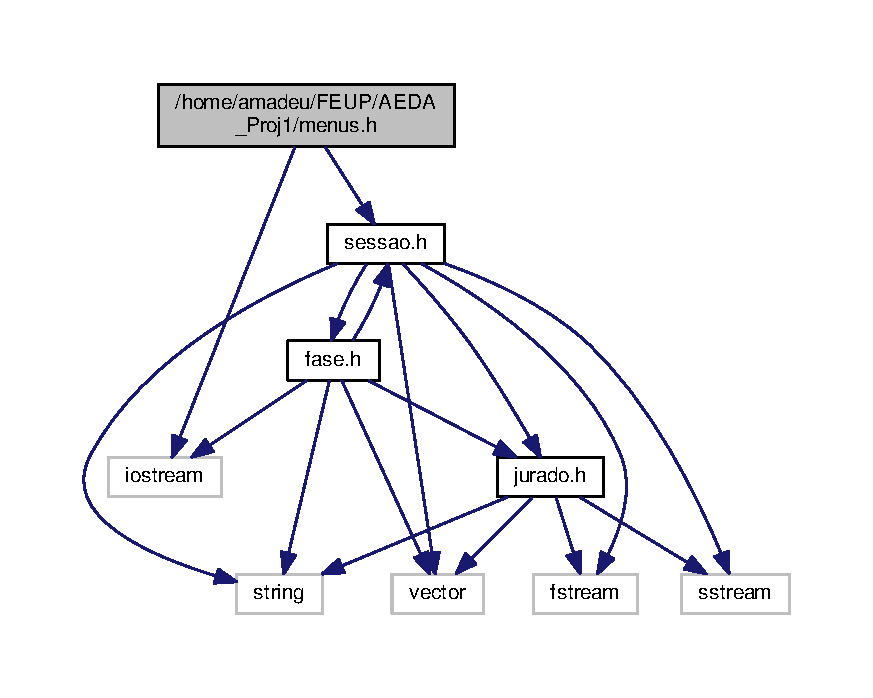
\includegraphics[width=350pt]{menus_8h__incl}
\end{center}
\end{figure}
This graph shows which files directly or indirectly include this file\+:
\nopagebreak
\begin{figure}[H]
\begin{center}
\leavevmode
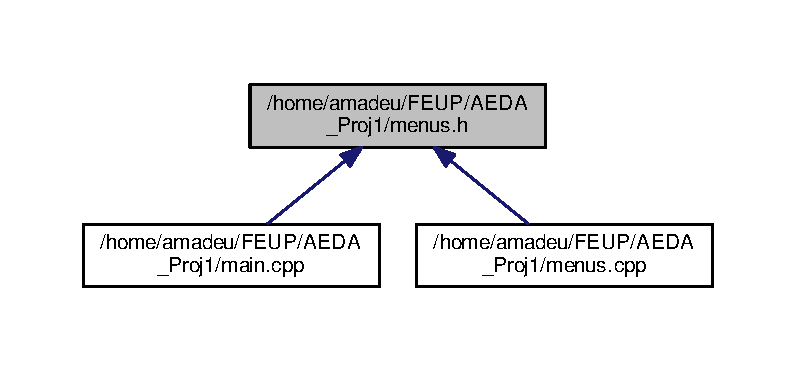
\includegraphics[width=350pt]{menus_8h__dep__incl}
\end{center}
\end{figure}
\subsection*{Functions}
\begin{DoxyCompactItemize}
\item 
void \hyperlink{menus_8h_a2a0e843767aeea4f433a28b9c54f573a}{menu} ()
\begin{DoxyCompactList}\small\item\em display do menu geral \end{DoxyCompactList}\item 
void \hyperlink{menus_8h_aab42b4271b882e2866f715920fcc5cef}{menu\+Candidatos} ()
\begin{DoxyCompactList}\small\item\em display do menu sobre os candidatos \end{DoxyCompactList}\item 
void \hyperlink{menus_8h_a9f532c9708d3f1997c55f6953bf652a4}{menu\+Jurados} ()
\begin{DoxyCompactList}\small\item\em display do menu sobre os jurados \end{DoxyCompactList}\item 
void \hyperlink{menus_8h_aeee7823bb4eb32e2795658999fde69e1}{menu\+Sessoes} ()
\begin{DoxyCompactList}\small\item\em display do menu acerca das varias sessoes \end{DoxyCompactList}\item 
void \hyperlink{menus_8h_a47dfe7486994b86baf402fc6be377475}{menu\+Adiciona\+Candidato} ()
\begin{DoxyCompactList}\small\item\em display do menu para adicionar um candidato \end{DoxyCompactList}\item 
void \hyperlink{menus_8h_a400dfb19e4bb59078fa09a4b184d22ef}{menu\+Remove\+Candidato} ()
\begin{DoxyCompactList}\small\item\em display do menu para remover um candidato \end{DoxyCompactList}\item 
void \hyperlink{menus_8h_a4ec260bdab29eb9b9637b39ef7dafa81}{menu\+Remove\+Candidato\+Numero} ()
\begin{DoxyCompactList}\small\item\em display do menu para remover um candidato com base no numero \end{DoxyCompactList}\item 
void \hyperlink{menus_8h_ad0a26823c8b0f7d0efc28c19c5685654}{menu\+Remove\+Candidato\+Nome} ()
\begin{DoxyCompactList}\small\item\em display do menu para remover um candidato com base no nome \end{DoxyCompactList}\item 
void \hyperlink{menus_8h_aea371219232565dc7858716a1bd47817}{menu\+Alterar\+Candidato} ()
\item 
void \hyperlink{menus_8h_a11b81ccf581a04e7630e65f8bd1bbbfa}{menu\+Alterar\+Candidato\+Numero} ()
\begin{DoxyCompactList}\small\item\em display do menu para alterar um candidato com base no numero \end{DoxyCompactList}\item 
void \hyperlink{menus_8h_aac0a29a50eef36bfd6ac7f627fa5bdec}{menu\+Alterar\+Candidato\+Nome} ()
\begin{DoxyCompactList}\small\item\em display do menu para alterar um candidato com base no nome \end{DoxyCompactList}\item 
void \hyperlink{menus_8h_ac2635799f82961fd2b0ec1f422967559}{menu\+Info\+Candidato} ()
\begin{DoxyCompactList}\small\item\em display do menu para ver a informacao dos candidatos \end{DoxyCompactList}\item 
void \hyperlink{menus_8h_a185fea948b263fa812288e236b2bd19a}{menu\+Info\+Candidato\+Numero} ()
\begin{DoxyCompactList}\small\item\em display do menu para procurar e ver a informacao de um candidato \end{DoxyCompactList}\item 
void \hyperlink{menus_8h_a2e5524ba2150e12fdabb7e0e42b5e940}{menu\+Info\+Candidatos\+Arte} ()
\begin{DoxyCompactList}\small\item\em display de todos os candidatos de uma arte perfomativa \end{DoxyCompactList}\item 
void \hyperlink{menus_8h_ae726400850a6789056a264558b233109}{menu\+Info\+Candidato\+Todos} ()
\begin{DoxyCompactList}\small\item\em display do menu para ver a informacao de todos os candidatos \end{DoxyCompactList}\item 
void \hyperlink{menus_8h_aa4f9c781fd709e6dff3db8cdbb2e27eb}{menu\+Adiciona\+Jurado} ()
\begin{DoxyCompactList}\small\item\em display do menu para adicionar um jurado \end{DoxyCompactList}\item 
void \hyperlink{menus_8h_a8ca47d3453fc44081302fdaac73c29f4}{menu\+Remove\+Jurado} ()
\begin{DoxyCompactList}\small\item\em display do menu para remover um jurado \end{DoxyCompactList}\item 
void \hyperlink{menus_8h_a69680649d07e58b0874bedeec5e00287}{menu\+Info\+Jurado} ()
\begin{DoxyCompactList}\small\item\em display do menu para ver a informacao dos candidatos \end{DoxyCompactList}\item 
void \hyperlink{menus_8h_ac8df289c83dac877629f7b11ae1f0947}{menu\+Info\+Jurado\+Nome} ()
\begin{DoxyCompactList}\small\item\em display do menu para procurar e ver a informacao de um jurado; \end{DoxyCompactList}\item 
void \hyperlink{menus_8h_a7d36bf5ec3b83ddb45a42760966be7b2}{menu\+Info\+Jurado\+Todos} ()
\begin{DoxyCompactList}\small\item\em display do menu para ver a informacao de todos os jurados \end{DoxyCompactList}\item 
void \hyperlink{menus_8h_a99f9a7afd9aeeb017fdf54b19fd223ef}{menu\+Adiciona\+Sessao} ()
\begin{DoxyCompactList}\small\item\em display do menu para adicionar uma sessao \end{DoxyCompactList}\item 
void \hyperlink{menus_8h_a93fea54aa1e26d7939776646bffc75ec}{menu\+Remove\+Sessao} ()
\begin{DoxyCompactList}\small\item\em display do menu para remover uma sessao \end{DoxyCompactList}\item 
void \hyperlink{menus_8h_ad8a0f4f72ff3592f271ceef3eb844185}{menu\+Adiciona\+Candidatos\+Sessao} (\hyperlink{classsessao}{sessao} $\ast$s)
\begin{DoxyCompactList}\small\item\em display do menu para adicionar candidatos a uma sessao \end{DoxyCompactList}\item 
int \hyperlink{menus_8h_a8555f02addba03c2b1f3702485995343}{menu\+Adiciona\+Jurados\+Sessao} (\hyperlink{classsessao}{sessao} $\ast$s)
\begin{DoxyCompactList}\small\item\em display do menu para adicionar jurados a uma sessao \end{DoxyCompactList}\item 
void \hyperlink{menus_8h_a47bc5591a007353eab848fbaf653447c}{menu\+Info\+Sessoes} ()
\begin{DoxyCompactList}\small\item\em display do menu para obter informacao de uma sessao \end{DoxyCompactList}\item 
void \hyperlink{menus_8h_a290c79dfdc80552b575fb89f0793d403}{menu\+Iniciar\+Sessao} ()
\end{DoxyCompactItemize}


\subsection{Function Documentation}
\index{menus.\+h@{menus.\+h}!menu@{menu}}
\index{menu@{menu}!menus.\+h@{menus.\+h}}
\subsubsection[{\texorpdfstring{menu()}{menu()}}]{\setlength{\rightskip}{0pt plus 5cm}void menu (
\begin{DoxyParamCaption}
{}
\end{DoxyParamCaption}
)}\hypertarget{menus_8h_a2a0e843767aeea4f433a28b9c54f573a}{}\label{menus_8h_a2a0e843767aeea4f433a28b9c54f573a}


display do menu geral 

\index{menus.\+h@{menus.\+h}!menu\+Adiciona\+Candidato@{menu\+Adiciona\+Candidato}}
\index{menu\+Adiciona\+Candidato@{menu\+Adiciona\+Candidato}!menus.\+h@{menus.\+h}}
\subsubsection[{\texorpdfstring{menu\+Adiciona\+Candidato()}{menuAdicionaCandidato()}}]{\setlength{\rightskip}{0pt plus 5cm}void menu\+Adiciona\+Candidato (
\begin{DoxyParamCaption}
{}
\end{DoxyParamCaption}
)}\hypertarget{menus_8h_a47dfe7486994b86baf402fc6be377475}{}\label{menus_8h_a47dfe7486994b86baf402fc6be377475}


display do menu para adicionar um candidato 

\index{menus.\+h@{menus.\+h}!menu\+Adiciona\+Candidatos\+Sessao@{menu\+Adiciona\+Candidatos\+Sessao}}
\index{menu\+Adiciona\+Candidatos\+Sessao@{menu\+Adiciona\+Candidatos\+Sessao}!menus.\+h@{menus.\+h}}
\subsubsection[{\texorpdfstring{menu\+Adiciona\+Candidatos\+Sessao(sessao $\ast$s)}{menuAdicionaCandidatosSessao(sessao *s)}}]{\setlength{\rightskip}{0pt plus 5cm}void menu\+Adiciona\+Candidatos\+Sessao (
\begin{DoxyParamCaption}
\item[{{\bf sessao} $\ast$}]{s}
\end{DoxyParamCaption}
)}\hypertarget{menus_8h_ad8a0f4f72ff3592f271ceef3eb844185}{}\label{menus_8h_ad8a0f4f72ff3592f271ceef3eb844185}


display do menu para adicionar candidatos a uma sessao 


\begin{DoxyParams}{Parameters}
{\em s} & sessao a que se pretende adicionar candidatos \\
\hline
\end{DoxyParams}
\index{menus.\+h@{menus.\+h}!menu\+Adiciona\+Jurado@{menu\+Adiciona\+Jurado}}
\index{menu\+Adiciona\+Jurado@{menu\+Adiciona\+Jurado}!menus.\+h@{menus.\+h}}
\subsubsection[{\texorpdfstring{menu\+Adiciona\+Jurado()}{menuAdicionaJurado()}}]{\setlength{\rightskip}{0pt plus 5cm}void menu\+Adiciona\+Jurado (
\begin{DoxyParamCaption}
{}
\end{DoxyParamCaption}
)}\hypertarget{menus_8h_aa4f9c781fd709e6dff3db8cdbb2e27eb}{}\label{menus_8h_aa4f9c781fd709e6dff3db8cdbb2e27eb}


display do menu para adicionar um jurado 

\index{menus.\+h@{menus.\+h}!menu\+Adiciona\+Jurados\+Sessao@{menu\+Adiciona\+Jurados\+Sessao}}
\index{menu\+Adiciona\+Jurados\+Sessao@{menu\+Adiciona\+Jurados\+Sessao}!menus.\+h@{menus.\+h}}
\subsubsection[{\texorpdfstring{menu\+Adiciona\+Jurados\+Sessao(sessao $\ast$s)}{menuAdicionaJuradosSessao(sessao *s)}}]{\setlength{\rightskip}{0pt plus 5cm}int menu\+Adiciona\+Jurados\+Sessao (
\begin{DoxyParamCaption}
\item[{{\bf sessao} $\ast$}]{s}
\end{DoxyParamCaption}
)}\hypertarget{menus_8h_a8555f02addba03c2b1f3702485995343}{}\label{menus_8h_a8555f02addba03c2b1f3702485995343}


display do menu para adicionar jurados a uma sessao 


\begin{DoxyParams}{Parameters}
{\em s} & sessao a que se pretende adicionar jurados \\
\hline
\end{DoxyParams}
\begin{DoxyReturn}{Returns}
devolve 1 se nao existirem jurados suficientes para criar uma sessao 
\end{DoxyReturn}
\index{menus.\+h@{menus.\+h}!menu\+Adiciona\+Sessao@{menu\+Adiciona\+Sessao}}
\index{menu\+Adiciona\+Sessao@{menu\+Adiciona\+Sessao}!menus.\+h@{menus.\+h}}
\subsubsection[{\texorpdfstring{menu\+Adiciona\+Sessao()}{menuAdicionaSessao()}}]{\setlength{\rightskip}{0pt plus 5cm}void menu\+Adiciona\+Sessao (
\begin{DoxyParamCaption}
{}
\end{DoxyParamCaption}
)}\hypertarget{menus_8h_a99f9a7afd9aeeb017fdf54b19fd223ef}{}\label{menus_8h_a99f9a7afd9aeeb017fdf54b19fd223ef}


display do menu para adicionar uma sessao 

\index{menus.\+h@{menus.\+h}!menu\+Alterar\+Candidato@{menu\+Alterar\+Candidato}}
\index{menu\+Alterar\+Candidato@{menu\+Alterar\+Candidato}!menus.\+h@{menus.\+h}}
\subsubsection[{\texorpdfstring{menu\+Alterar\+Candidato()}{menuAlterarCandidato()}}]{\setlength{\rightskip}{0pt plus 5cm}void menu\+Alterar\+Candidato (
\begin{DoxyParamCaption}
{}
\end{DoxyParamCaption}
)}\hypertarget{menus_8h_aea371219232565dc7858716a1bd47817}{}\label{menus_8h_aea371219232565dc7858716a1bd47817}
display do menu para alterar a informacao de um candidato \index{menus.\+h@{menus.\+h}!menu\+Alterar\+Candidato\+Nome@{menu\+Alterar\+Candidato\+Nome}}
\index{menu\+Alterar\+Candidato\+Nome@{menu\+Alterar\+Candidato\+Nome}!menus.\+h@{menus.\+h}}
\subsubsection[{\texorpdfstring{menu\+Alterar\+Candidato\+Nome()}{menuAlterarCandidatoNome()}}]{\setlength{\rightskip}{0pt plus 5cm}void menu\+Alterar\+Candidato\+Nome (
\begin{DoxyParamCaption}
{}
\end{DoxyParamCaption}
)}\hypertarget{menus_8h_aac0a29a50eef36bfd6ac7f627fa5bdec}{}\label{menus_8h_aac0a29a50eef36bfd6ac7f627fa5bdec}


display do menu para alterar um candidato com base no nome 

\index{menus.\+h@{menus.\+h}!menu\+Alterar\+Candidato\+Numero@{menu\+Alterar\+Candidato\+Numero}}
\index{menu\+Alterar\+Candidato\+Numero@{menu\+Alterar\+Candidato\+Numero}!menus.\+h@{menus.\+h}}
\subsubsection[{\texorpdfstring{menu\+Alterar\+Candidato\+Numero()}{menuAlterarCandidatoNumero()}}]{\setlength{\rightskip}{0pt plus 5cm}void menu\+Alterar\+Candidato\+Numero (
\begin{DoxyParamCaption}
{}
\end{DoxyParamCaption}
)}\hypertarget{menus_8h_a11b81ccf581a04e7630e65f8bd1bbbfa}{}\label{menus_8h_a11b81ccf581a04e7630e65f8bd1bbbfa}


display do menu para alterar um candidato com base no numero 

\index{menus.\+h@{menus.\+h}!menu\+Candidatos@{menu\+Candidatos}}
\index{menu\+Candidatos@{menu\+Candidatos}!menus.\+h@{menus.\+h}}
\subsubsection[{\texorpdfstring{menu\+Candidatos()}{menuCandidatos()}}]{\setlength{\rightskip}{0pt plus 5cm}void menu\+Candidatos (
\begin{DoxyParamCaption}
{}
\end{DoxyParamCaption}
)}\hypertarget{menus_8h_aab42b4271b882e2866f715920fcc5cef}{}\label{menus_8h_aab42b4271b882e2866f715920fcc5cef}


display do menu sobre os candidatos 

\index{menus.\+h@{menus.\+h}!menu\+Info\+Candidato@{menu\+Info\+Candidato}}
\index{menu\+Info\+Candidato@{menu\+Info\+Candidato}!menus.\+h@{menus.\+h}}
\subsubsection[{\texorpdfstring{menu\+Info\+Candidato()}{menuInfoCandidato()}}]{\setlength{\rightskip}{0pt plus 5cm}void menu\+Info\+Candidato (
\begin{DoxyParamCaption}
{}
\end{DoxyParamCaption}
)}\hypertarget{menus_8h_ac2635799f82961fd2b0ec1f422967559}{}\label{menus_8h_ac2635799f82961fd2b0ec1f422967559}


display do menu para ver a informacao dos candidatos 

\index{menus.\+h@{menus.\+h}!menu\+Info\+Candidato\+Numero@{menu\+Info\+Candidato\+Numero}}
\index{menu\+Info\+Candidato\+Numero@{menu\+Info\+Candidato\+Numero}!menus.\+h@{menus.\+h}}
\subsubsection[{\texorpdfstring{menu\+Info\+Candidato\+Numero()}{menuInfoCandidatoNumero()}}]{\setlength{\rightskip}{0pt plus 5cm}void menu\+Info\+Candidato\+Numero (
\begin{DoxyParamCaption}
{}
\end{DoxyParamCaption}
)}\hypertarget{menus_8h_a185fea948b263fa812288e236b2bd19a}{}\label{menus_8h_a185fea948b263fa812288e236b2bd19a}


display do menu para procurar e ver a informacao de um candidato 

\index{menus.\+h@{menus.\+h}!menu\+Info\+Candidatos\+Arte@{menu\+Info\+Candidatos\+Arte}}
\index{menu\+Info\+Candidatos\+Arte@{menu\+Info\+Candidatos\+Arte}!menus.\+h@{menus.\+h}}
\subsubsection[{\texorpdfstring{menu\+Info\+Candidatos\+Arte()}{menuInfoCandidatosArte()}}]{\setlength{\rightskip}{0pt plus 5cm}void menu\+Info\+Candidatos\+Arte (
\begin{DoxyParamCaption}
{}
\end{DoxyParamCaption}
)}\hypertarget{menus_8h_a2e5524ba2150e12fdabb7e0e42b5e940}{}\label{menus_8h_a2e5524ba2150e12fdabb7e0e42b5e940}


display de todos os candidatos de uma arte perfomativa 

\index{menus.\+h@{menus.\+h}!menu\+Info\+Candidato\+Todos@{menu\+Info\+Candidato\+Todos}}
\index{menu\+Info\+Candidato\+Todos@{menu\+Info\+Candidato\+Todos}!menus.\+h@{menus.\+h}}
\subsubsection[{\texorpdfstring{menu\+Info\+Candidato\+Todos()}{menuInfoCandidatoTodos()}}]{\setlength{\rightskip}{0pt plus 5cm}void menu\+Info\+Candidato\+Todos (
\begin{DoxyParamCaption}
{}
\end{DoxyParamCaption}
)}\hypertarget{menus_8h_ae726400850a6789056a264558b233109}{}\label{menus_8h_ae726400850a6789056a264558b233109}


display do menu para ver a informacao de todos os candidatos 

\index{menus.\+h@{menus.\+h}!menu\+Info\+Jurado@{menu\+Info\+Jurado}}
\index{menu\+Info\+Jurado@{menu\+Info\+Jurado}!menus.\+h@{menus.\+h}}
\subsubsection[{\texorpdfstring{menu\+Info\+Jurado()}{menuInfoJurado()}}]{\setlength{\rightskip}{0pt plus 5cm}void menu\+Info\+Jurado (
\begin{DoxyParamCaption}
{}
\end{DoxyParamCaption}
)}\hypertarget{menus_8h_a69680649d07e58b0874bedeec5e00287}{}\label{menus_8h_a69680649d07e58b0874bedeec5e00287}


display do menu para ver a informacao dos candidatos 

\index{menus.\+h@{menus.\+h}!menu\+Info\+Jurado\+Nome@{menu\+Info\+Jurado\+Nome}}
\index{menu\+Info\+Jurado\+Nome@{menu\+Info\+Jurado\+Nome}!menus.\+h@{menus.\+h}}
\subsubsection[{\texorpdfstring{menu\+Info\+Jurado\+Nome()}{menuInfoJuradoNome()}}]{\setlength{\rightskip}{0pt plus 5cm}void menu\+Info\+Jurado\+Nome (
\begin{DoxyParamCaption}
{}
\end{DoxyParamCaption}
)}\hypertarget{menus_8h_ac8df289c83dac877629f7b11ae1f0947}{}\label{menus_8h_ac8df289c83dac877629f7b11ae1f0947}


display do menu para procurar e ver a informacao de um jurado; 

\index{menus.\+h@{menus.\+h}!menu\+Info\+Jurado\+Todos@{menu\+Info\+Jurado\+Todos}}
\index{menu\+Info\+Jurado\+Todos@{menu\+Info\+Jurado\+Todos}!menus.\+h@{menus.\+h}}
\subsubsection[{\texorpdfstring{menu\+Info\+Jurado\+Todos()}{menuInfoJuradoTodos()}}]{\setlength{\rightskip}{0pt plus 5cm}void menu\+Info\+Jurado\+Todos (
\begin{DoxyParamCaption}
{}
\end{DoxyParamCaption}
)}\hypertarget{menus_8h_a7d36bf5ec3b83ddb45a42760966be7b2}{}\label{menus_8h_a7d36bf5ec3b83ddb45a42760966be7b2}


display do menu para ver a informacao de todos os jurados 

\index{menus.\+h@{menus.\+h}!menu\+Info\+Sessoes@{menu\+Info\+Sessoes}}
\index{menu\+Info\+Sessoes@{menu\+Info\+Sessoes}!menus.\+h@{menus.\+h}}
\subsubsection[{\texorpdfstring{menu\+Info\+Sessoes()}{menuInfoSessoes()}}]{\setlength{\rightskip}{0pt plus 5cm}void menu\+Info\+Sessoes (
\begin{DoxyParamCaption}
{}
\end{DoxyParamCaption}
)}\hypertarget{menus_8h_a47bc5591a007353eab848fbaf653447c}{}\label{menus_8h_a47bc5591a007353eab848fbaf653447c}


display do menu para obter informacao de uma sessao 

\index{menus.\+h@{menus.\+h}!menu\+Iniciar\+Sessao@{menu\+Iniciar\+Sessao}}
\index{menu\+Iniciar\+Sessao@{menu\+Iniciar\+Sessao}!menus.\+h@{menus.\+h}}
\subsubsection[{\texorpdfstring{menu\+Iniciar\+Sessao()}{menuIniciarSessao()}}]{\setlength{\rightskip}{0pt plus 5cm}void menu\+Iniciar\+Sessao (
\begin{DoxyParamCaption}
{}
\end{DoxyParamCaption}
)}\hypertarget{menus_8h_a290c79dfdc80552b575fb89f0793d403}{}\label{menus_8h_a290c79dfdc80552b575fb89f0793d403}
\index{menus.\+h@{menus.\+h}!menu\+Jurados@{menu\+Jurados}}
\index{menu\+Jurados@{menu\+Jurados}!menus.\+h@{menus.\+h}}
\subsubsection[{\texorpdfstring{menu\+Jurados()}{menuJurados()}}]{\setlength{\rightskip}{0pt plus 5cm}void menu\+Jurados (
\begin{DoxyParamCaption}
{}
\end{DoxyParamCaption}
)}\hypertarget{menus_8h_a9f532c9708d3f1997c55f6953bf652a4}{}\label{menus_8h_a9f532c9708d3f1997c55f6953bf652a4}


display do menu sobre os jurados 

\index{menus.\+h@{menus.\+h}!menu\+Remove\+Candidato@{menu\+Remove\+Candidato}}
\index{menu\+Remove\+Candidato@{menu\+Remove\+Candidato}!menus.\+h@{menus.\+h}}
\subsubsection[{\texorpdfstring{menu\+Remove\+Candidato()}{menuRemoveCandidato()}}]{\setlength{\rightskip}{0pt plus 5cm}void menu\+Remove\+Candidato (
\begin{DoxyParamCaption}
{}
\end{DoxyParamCaption}
)}\hypertarget{menus_8h_a400dfb19e4bb59078fa09a4b184d22ef}{}\label{menus_8h_a400dfb19e4bb59078fa09a4b184d22ef}


display do menu para remover um candidato 

\index{menus.\+h@{menus.\+h}!menu\+Remove\+Candidato\+Nome@{menu\+Remove\+Candidato\+Nome}}
\index{menu\+Remove\+Candidato\+Nome@{menu\+Remove\+Candidato\+Nome}!menus.\+h@{menus.\+h}}
\subsubsection[{\texorpdfstring{menu\+Remove\+Candidato\+Nome()}{menuRemoveCandidatoNome()}}]{\setlength{\rightskip}{0pt plus 5cm}void menu\+Remove\+Candidato\+Nome (
\begin{DoxyParamCaption}
{}
\end{DoxyParamCaption}
)}\hypertarget{menus_8h_ad0a26823c8b0f7d0efc28c19c5685654}{}\label{menus_8h_ad0a26823c8b0f7d0efc28c19c5685654}


display do menu para remover um candidato com base no nome 

\index{menus.\+h@{menus.\+h}!menu\+Remove\+Candidato\+Numero@{menu\+Remove\+Candidato\+Numero}}
\index{menu\+Remove\+Candidato\+Numero@{menu\+Remove\+Candidato\+Numero}!menus.\+h@{menus.\+h}}
\subsubsection[{\texorpdfstring{menu\+Remove\+Candidato\+Numero()}{menuRemoveCandidatoNumero()}}]{\setlength{\rightskip}{0pt plus 5cm}void menu\+Remove\+Candidato\+Numero (
\begin{DoxyParamCaption}
{}
\end{DoxyParamCaption}
)}\hypertarget{menus_8h_a4ec260bdab29eb9b9637b39ef7dafa81}{}\label{menus_8h_a4ec260bdab29eb9b9637b39ef7dafa81}


display do menu para remover um candidato com base no numero 

\index{menus.\+h@{menus.\+h}!menu\+Remove\+Jurado@{menu\+Remove\+Jurado}}
\index{menu\+Remove\+Jurado@{menu\+Remove\+Jurado}!menus.\+h@{menus.\+h}}
\subsubsection[{\texorpdfstring{menu\+Remove\+Jurado()}{menuRemoveJurado()}}]{\setlength{\rightskip}{0pt plus 5cm}void menu\+Remove\+Jurado (
\begin{DoxyParamCaption}
{}
\end{DoxyParamCaption}
)}\hypertarget{menus_8h_a8ca47d3453fc44081302fdaac73c29f4}{}\label{menus_8h_a8ca47d3453fc44081302fdaac73c29f4}


display do menu para remover um jurado 

\index{menus.\+h@{menus.\+h}!menu\+Remove\+Sessao@{menu\+Remove\+Sessao}}
\index{menu\+Remove\+Sessao@{menu\+Remove\+Sessao}!menus.\+h@{menus.\+h}}
\subsubsection[{\texorpdfstring{menu\+Remove\+Sessao()}{menuRemoveSessao()}}]{\setlength{\rightskip}{0pt plus 5cm}void menu\+Remove\+Sessao (
\begin{DoxyParamCaption}
{}
\end{DoxyParamCaption}
)}\hypertarget{menus_8h_a93fea54aa1e26d7939776646bffc75ec}{}\label{menus_8h_a93fea54aa1e26d7939776646bffc75ec}


display do menu para remover uma sessao 

\index{menus.\+h@{menus.\+h}!menu\+Sessoes@{menu\+Sessoes}}
\index{menu\+Sessoes@{menu\+Sessoes}!menus.\+h@{menus.\+h}}
\subsubsection[{\texorpdfstring{menu\+Sessoes()}{menuSessoes()}}]{\setlength{\rightskip}{0pt plus 5cm}void menu\+Sessoes (
\begin{DoxyParamCaption}
{}
\end{DoxyParamCaption}
)}\hypertarget{menus_8h_aeee7823bb4eb32e2795658999fde69e1}{}\label{menus_8h_aeee7823bb4eb32e2795658999fde69e1}


display do menu acerca das varias sessoes 


\hypertarget{sessao_8cpp}{}\section{/home/amadeu/\+F\+E\+U\+P/\+A\+E\+D\+A\+\_\+\+Proj1/sessao.cpp File Reference}
\label{sessao_8cpp}\index{/home/amadeu/\+F\+E\+U\+P/\+A\+E\+D\+A\+\_\+\+Proj1/sessao.\+cpp@{/home/amadeu/\+F\+E\+U\+P/\+A\+E\+D\+A\+\_\+\+Proj1/sessao.\+cpp}}
{\ttfamily \#include \char`\"{}sessao.\+h\char`\"{}}\\*
{\ttfamily \#include \char`\"{}funcoes.\+h\char`\"{}}\\*
Include dependency graph for sessao.\+cpp\+:
\nopagebreak
\begin{figure}[H]
\begin{center}
\leavevmode
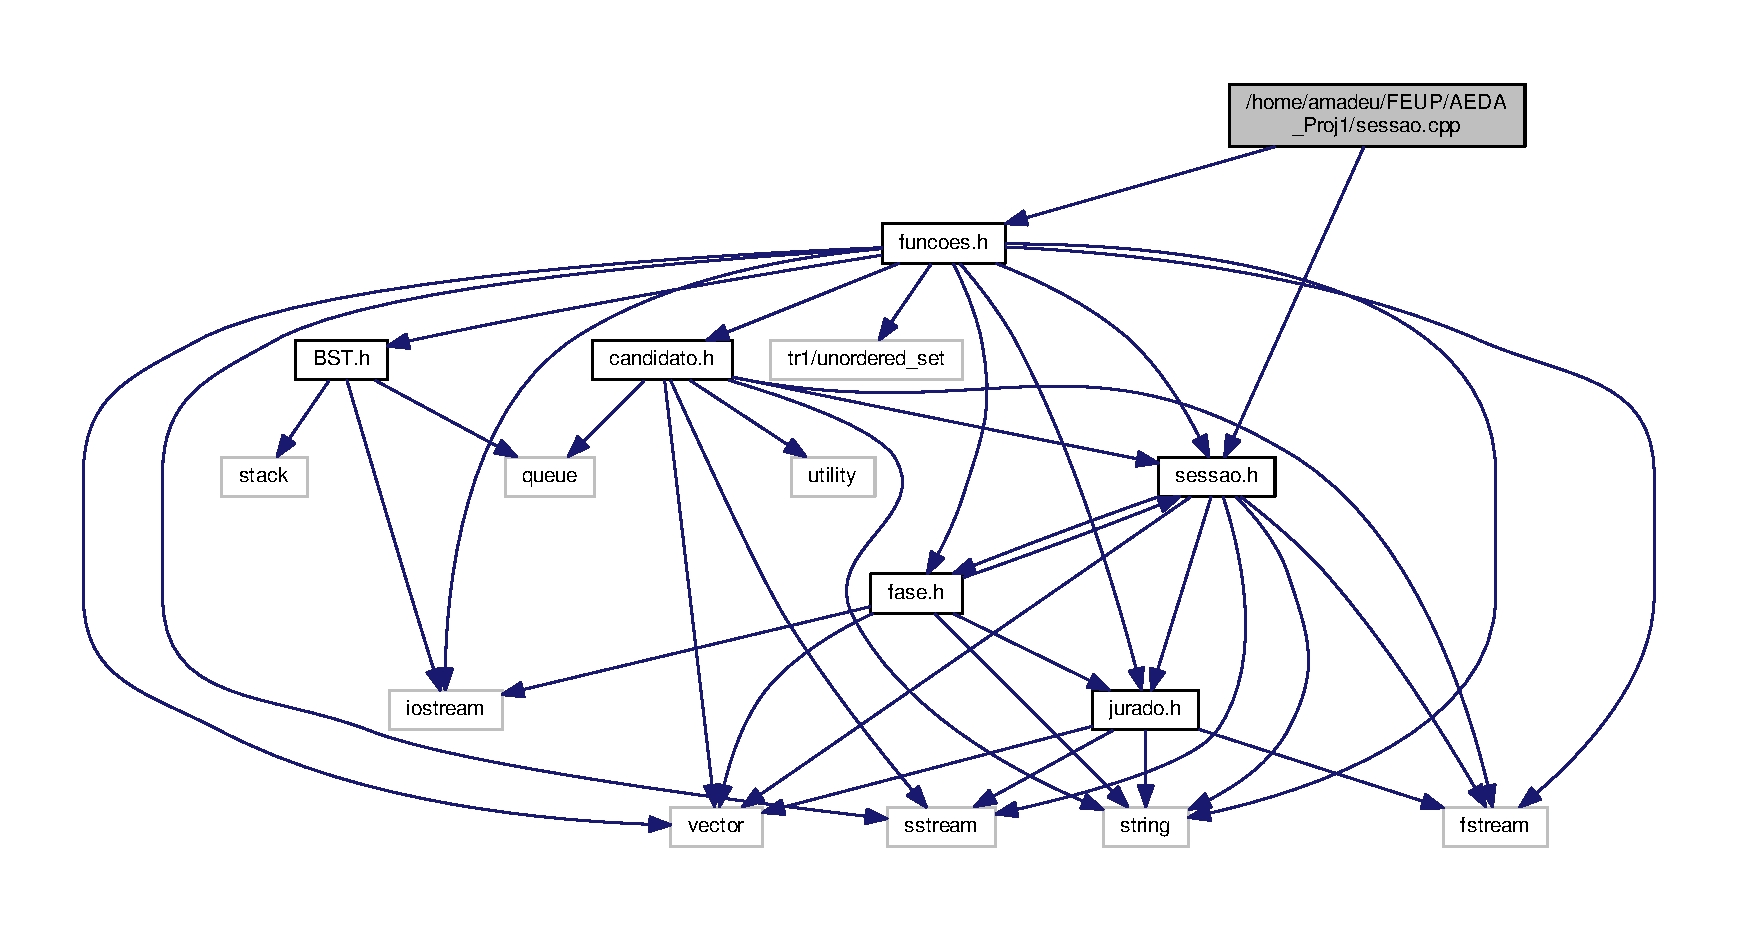
\includegraphics[width=350pt]{sessao_8cpp__incl}
\end{center}
\end{figure}
\subsection*{Functions}
\begin{DoxyCompactItemize}
\item 
ostream \& \hyperlink{sessao_8cpp_ae6b6ae8802a28ad9208f2af03f14a056}{operator$<$$<$} (std\+::ostream \&out, const \hyperlink{classsessaoJaExiste}{sessao\+Ja\+Existe} \&s)
\item 
std\+::ostream \& \hyperlink{sessao_8cpp_aba9476f9a49d32df37a5021851d372c8}{operator$<$$<$} (std\+::ostream \&out, const \hyperlink{classsessaoNaoExiste}{sessao\+Nao\+Existe} \&s)
\item 
ostream \& \hyperlink{sessao_8cpp_a442be9403858cf93de76510cccc64496}{operator$<$$<$} (ostream \&o, const \hyperlink{classsessao}{sessao} $\ast$s)
\item 
ofstream \& \hyperlink{sessao_8cpp_ac46d6bce5998eb1597ae5866c39938c5}{operator$<$$<$} (ofstream \&o, const \hyperlink{classsessao}{sessao} $\ast$s)
\end{DoxyCompactItemize}


\subsection{Function Documentation}
\index{sessao.\+cpp@{sessao.\+cpp}!operator$<$$<$@{operator$<$$<$}}
\index{operator$<$$<$@{operator$<$$<$}!sessao.\+cpp@{sessao.\+cpp}}
\subsubsection[{\texorpdfstring{operator$<$$<$(std\+::ostream \&out, const sessao\+Ja\+Existe \&s)}{operator<<(std::ostream &out, const sessaoJaExiste &s)}}]{\setlength{\rightskip}{0pt plus 5cm}ostream\& operator$<$$<$ (
\begin{DoxyParamCaption}
\item[{std\+::ostream \&}]{out, }
\item[{const {\bf sessao\+Ja\+Existe} \&}]{s}
\end{DoxyParamCaption}
)}\hypertarget{sessao_8cpp_ae6b6ae8802a28ad9208f2af03f14a056}{}\label{sessao_8cpp_ae6b6ae8802a28ad9208f2af03f14a056}
\index{sessao.\+cpp@{sessao.\+cpp}!operator$<$$<$@{operator$<$$<$}}
\index{operator$<$$<$@{operator$<$$<$}!sessao.\+cpp@{sessao.\+cpp}}
\subsubsection[{\texorpdfstring{operator$<$$<$(std\+::ostream \&out, const sessao\+Nao\+Existe \&s)}{operator<<(std::ostream &out, const sessaoNaoExiste &s)}}]{\setlength{\rightskip}{0pt plus 5cm}std\+::ostream\& operator$<$$<$ (
\begin{DoxyParamCaption}
\item[{std\+::ostream \&}]{out, }
\item[{const {\bf sessao\+Nao\+Existe} \&}]{s}
\end{DoxyParamCaption}
)}\hypertarget{sessao_8cpp_aba9476f9a49d32df37a5021851d372c8}{}\label{sessao_8cpp_aba9476f9a49d32df37a5021851d372c8}
\index{sessao.\+cpp@{sessao.\+cpp}!operator$<$$<$@{operator$<$$<$}}
\index{operator$<$$<$@{operator$<$$<$}!sessao.\+cpp@{sessao.\+cpp}}
\subsubsection[{\texorpdfstring{operator$<$$<$(ostream \&o, const sessao $\ast$s)}{operator<<(ostream &o, const sessao *s)}}]{\setlength{\rightskip}{0pt plus 5cm}ostream\& operator$<$$<$ (
\begin{DoxyParamCaption}
\item[{ostream \&}]{o, }
\item[{const {\bf sessao} $\ast$}]{s}
\end{DoxyParamCaption}
)}\hypertarget{sessao_8cpp_a442be9403858cf93de76510cccc64496}{}\label{sessao_8cpp_a442be9403858cf93de76510cccc64496}
\index{sessao.\+cpp@{sessao.\+cpp}!operator$<$$<$@{operator$<$$<$}}
\index{operator$<$$<$@{operator$<$$<$}!sessao.\+cpp@{sessao.\+cpp}}
\subsubsection[{\texorpdfstring{operator$<$$<$(ofstream \&o, const sessao $\ast$s)}{operator<<(ofstream &o, const sessao *s)}}]{\setlength{\rightskip}{0pt plus 5cm}ofstream\& operator$<$$<$ (
\begin{DoxyParamCaption}
\item[{ofstream \&}]{o, }
\item[{const {\bf sessao} $\ast$}]{s}
\end{DoxyParamCaption}
)}\hypertarget{sessao_8cpp_ac46d6bce5998eb1597ae5866c39938c5}{}\label{sessao_8cpp_ac46d6bce5998eb1597ae5866c39938c5}

\hypertarget{sessao_8h}{}\section{/home/amadeu/\+F\+E\+U\+P/\+A\+E\+D\+A\+\_\+\+Proj1/sessao.h File Reference}
\label{sessao_8h}\index{/home/amadeu/\+F\+E\+U\+P/\+A\+E\+D\+A\+\_\+\+Proj1/sessao.\+h@{/home/amadeu/\+F\+E\+U\+P/\+A\+E\+D\+A\+\_\+\+Proj1/sessao.\+h}}
{\ttfamily \#include $<$string$>$}\\*
{\ttfamily \#include $<$vector$>$}\\*
{\ttfamily \#include $<$fstream$>$}\\*
{\ttfamily \#include $<$sstream$>$}\\*
{\ttfamily \#include \char`\"{}jurado.\+h\char`\"{}}\\*
{\ttfamily \#include \char`\"{}fase.\+h\char`\"{}}\\*
Include dependency graph for sessao.\+h\+:
\nopagebreak
\begin{figure}[H]
\begin{center}
\leavevmode
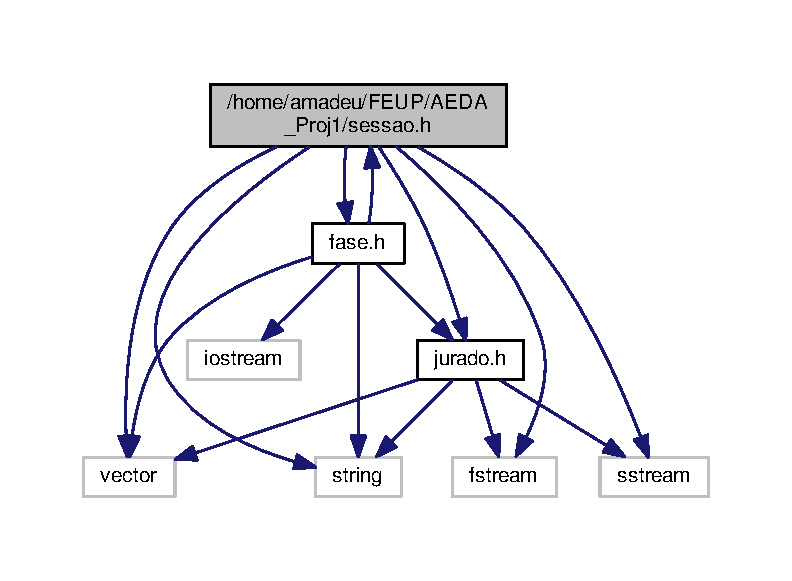
\includegraphics[width=350pt]{sessao_8h__incl}
\end{center}
\end{figure}
This graph shows which files directly or indirectly include this file\+:
\nopagebreak
\begin{figure}[H]
\begin{center}
\leavevmode
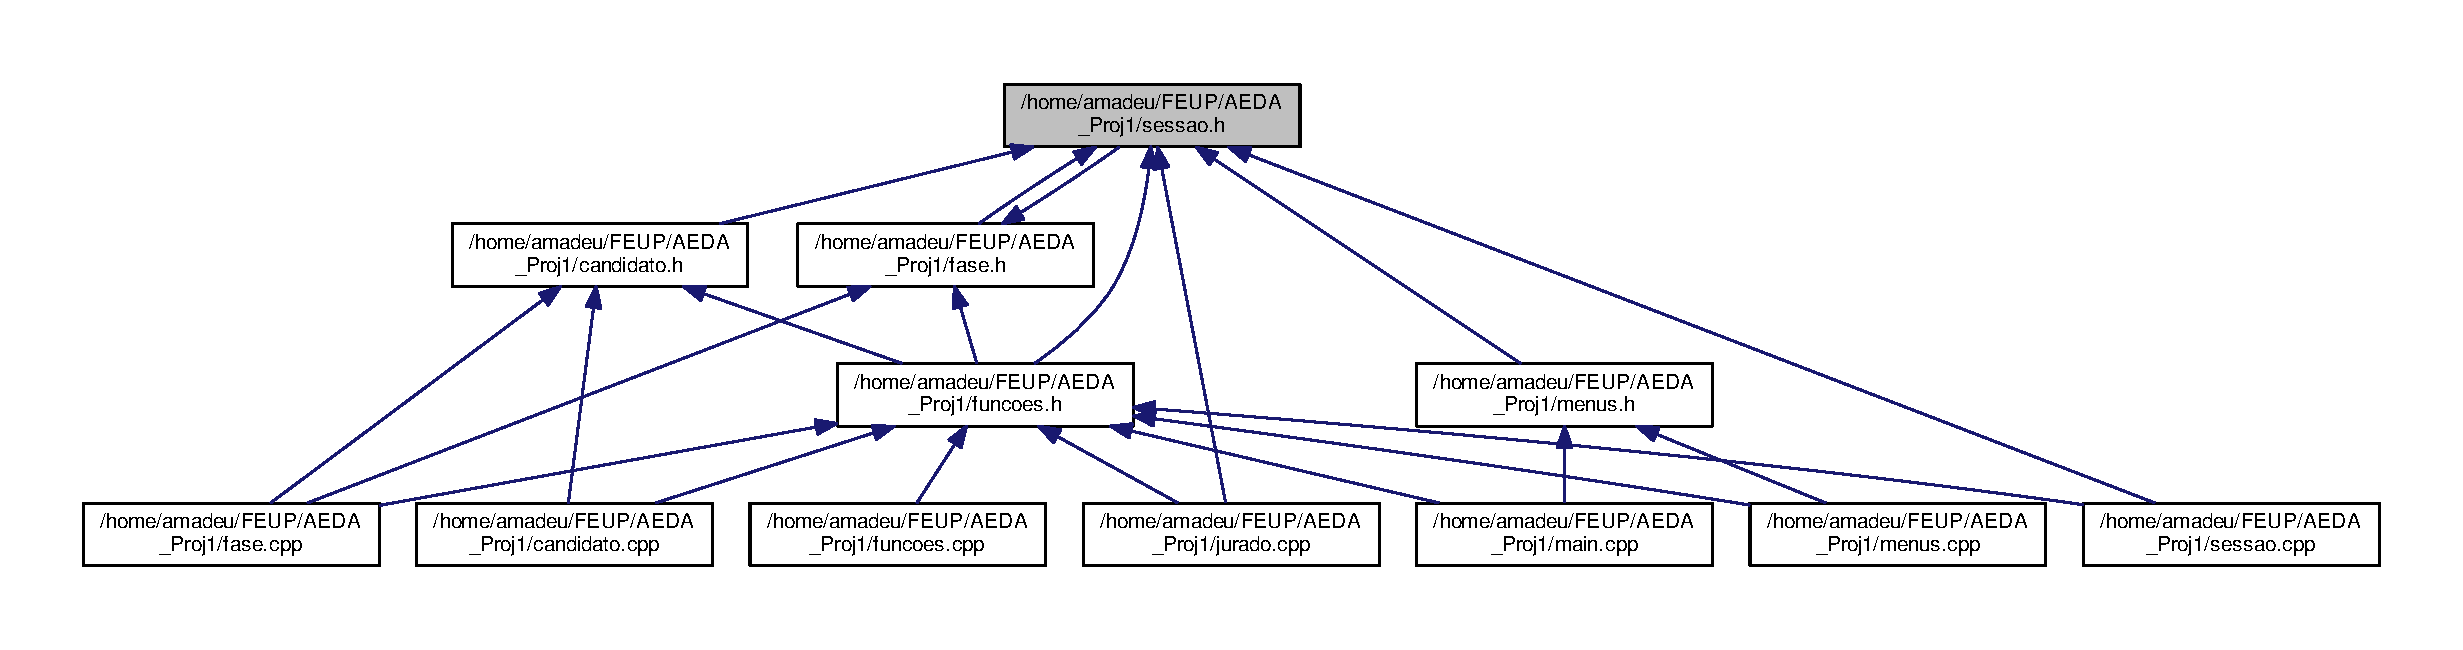
\includegraphics[width=350pt]{sessao_8h__dep__incl}
\end{center}
\end{figure}
\subsection*{Classes}
\begin{DoxyCompactItemize}
\item 
class \hyperlink{classsessao}{sessao}
\begin{DoxyCompactList}\small\item\em classe com as informacoes relativas a uma sessao \end{DoxyCompactList}\item 
class \hyperlink{classsessaoNaoExiste}{sessao\+Nao\+Existe}
\begin{DoxyCompactList}\small\item\em excepcao para quando um objeto da classe sessao nao existe \end{DoxyCompactList}\item 
class \hyperlink{classsessaoJaExiste}{sessao\+Ja\+Existe}
\begin{DoxyCompactList}\small\item\em excepcao para quando um objeto da classe sessao ja existe \end{DoxyCompactList}\end{DoxyCompactItemize}
\subsection*{Functions}
\begin{DoxyCompactItemize}
\item 
std\+::ostream \& \hyperlink{sessao_8h_aba9476f9a49d32df37a5021851d372c8}{operator$<$$<$} (std\+::ostream \&out, const \hyperlink{classsessaoNaoExiste}{sessao\+Nao\+Existe} \&s)
\item 
std\+::ostream \& \hyperlink{sessao_8h_a6cdccaf6493a09d18af4afe5d7075797}{operator$<$$<$} (std\+::ostream \&out, const \hyperlink{classsessaoJaExiste}{sessao\+Ja\+Existe} \&s)
\end{DoxyCompactItemize}


\subsection{Function Documentation}
\index{sessao.\+h@{sessao.\+h}!operator$<$$<$@{operator$<$$<$}}
\index{operator$<$$<$@{operator$<$$<$}!sessao.\+h@{sessao.\+h}}
\subsubsection[{\texorpdfstring{operator$<$$<$(std\+::ostream \&out, const sessao\+Nao\+Existe \&s)}{operator<<(std::ostream &out, const sessaoNaoExiste &s)}}]{\setlength{\rightskip}{0pt plus 5cm}std\+::ostream\& operator$<$$<$ (
\begin{DoxyParamCaption}
\item[{std\+::ostream \&}]{out, }
\item[{const {\bf sessao\+Nao\+Existe} \&}]{s}
\end{DoxyParamCaption}
)}\hypertarget{sessao_8h_aba9476f9a49d32df37a5021851d372c8}{}\label{sessao_8h_aba9476f9a49d32df37a5021851d372c8}
\index{sessao.\+h@{sessao.\+h}!operator$<$$<$@{operator$<$$<$}}
\index{operator$<$$<$@{operator$<$$<$}!sessao.\+h@{sessao.\+h}}
\subsubsection[{\texorpdfstring{operator$<$$<$(std\+::ostream \&out, const sessao\+Ja\+Existe \&s)}{operator<<(std::ostream &out, const sessaoJaExiste &s)}}]{\setlength{\rightskip}{0pt plus 5cm}std\+::ostream\& operator$<$$<$ (
\begin{DoxyParamCaption}
\item[{std\+::ostream \&}]{out, }
\item[{const {\bf sessao\+Ja\+Existe} \&}]{s}
\end{DoxyParamCaption}
)}\hypertarget{sessao_8h_a6cdccaf6493a09d18af4afe5d7075797}{}\label{sessao_8h_a6cdccaf6493a09d18af4afe5d7075797}

\hypertarget{sessoes_8txt}{}\section{/home/amadeu/\+F\+E\+U\+P/\+A\+E\+D\+A\+\_\+\+Proj1/sessoes.txt File Reference}
\label{sessoes_8txt}\index{/home/amadeu/\+F\+E\+U\+P/\+A\+E\+D\+A\+\_\+\+Proj1/sessoes.\+txt@{/home/amadeu/\+F\+E\+U\+P/\+A\+E\+D\+A\+\_\+\+Proj1/sessoes.\+txt}}
\subsection*{Variables}
\begin{DoxyCompactItemize}
\item 
\hyperlink{sessoes_8txt_a2616159a76d0e8a5493734758ae9c160}{cantar}
\item 
\hyperlink{sessoes_8txt_a766f9ab60ec18d5b80bf4153a38c2b64}{Marta}
\item 
\hyperlink{sessoes_8txt_a83ec618410e4714b08aa56507a10f025}{Pedro}
\item 
\hyperlink{sessoes_8txt_ae102a7586632535be9ea3d3f64768ab4}{Rui}
\item 
\hyperlink{sessoes_8txt_a6414eb73c2395148093f8baa9e202616}{Joao}
\item 
\hyperlink{sessoes_8txt_a8c64f18bebe8b957cbc75ce757dd3af4}{Carlos}
\item 
\hyperlink{sessoes_8txt_a508a855615268f4003a2dcef768b5abe}{Ricardo}
\item 
\hyperlink{sessoes_8txt_abc15862bdb1800c6fcdf948e0de62523}{Helena}
\item 
\hyperlink{sessoes_8txt_adb78776c95ad5bfba2eb9fce119157de}{magia}
\item 
\hyperlink{sessoes_8txt_a13cbd16d251cdd3a5b7719091bb517a7}{Jose}
\item 
\hyperlink{sessoes_8txt_aeb25d2279e6bf681577196df60fd4618}{Alexandra}
\item 
\hyperlink{sessoes_8txt_af582cac3444e41dc13a517bd4e6efbd7}{Miguel}
\item 
\hyperlink{sessoes_8txt_a7649ba4017592bd762abe5b976e6481e}{dancar}
\item 
\hyperlink{sessoes_8txt_aff6a0439a2c5c374e2852843155c2df4}{Raquel}
\item 
\hyperlink{sessoes_8txt_a0375353ca858a7b935ff53ef0a3c9a98}{Maria}
\item 
\hyperlink{sessoes_8txt_a33e5ff5ddbb7118468c3dd458466532b}{Bruno}
\item 
\hyperlink{sessoes_8txt_a8f0142e65cd12bdd0d475a7c68a99433}{Antonio}
\end{DoxyCompactItemize}


\subsection{Variable Documentation}
\index{sessoes.\+txt@{sessoes.\+txt}!Alexandra@{Alexandra}}
\index{Alexandra@{Alexandra}!sessoes.\+txt@{sessoes.\+txt}}
\subsubsection[{\texorpdfstring{Alexandra}{Alexandra}}]{\setlength{\rightskip}{0pt plus 5cm}Alexandra}\hypertarget{sessoes_8txt_aeb25d2279e6bf681577196df60fd4618}{}\label{sessoes_8txt_aeb25d2279e6bf681577196df60fd4618}
\index{sessoes.\+txt@{sessoes.\+txt}!Antonio@{Antonio}}
\index{Antonio@{Antonio}!sessoes.\+txt@{sessoes.\+txt}}
\subsubsection[{\texorpdfstring{Antonio}{Antonio}}]{\setlength{\rightskip}{0pt plus 5cm}Antonio}\hypertarget{sessoes_8txt_a8f0142e65cd12bdd0d475a7c68a99433}{}\label{sessoes_8txt_a8f0142e65cd12bdd0d475a7c68a99433}
\index{sessoes.\+txt@{sessoes.\+txt}!Bruno@{Bruno}}
\index{Bruno@{Bruno}!sessoes.\+txt@{sessoes.\+txt}}
\subsubsection[{\texorpdfstring{Bruno}{Bruno}}]{\setlength{\rightskip}{0pt plus 5cm}Bruno}\hypertarget{sessoes_8txt_a33e5ff5ddbb7118468c3dd458466532b}{}\label{sessoes_8txt_a33e5ff5ddbb7118468c3dd458466532b}
\index{sessoes.\+txt@{sessoes.\+txt}!cantar@{cantar}}
\index{cantar@{cantar}!sessoes.\+txt@{sessoes.\+txt}}
\subsubsection[{\texorpdfstring{cantar}{cantar}}]{\setlength{\rightskip}{0pt plus 5cm}cantar}\hypertarget{sessoes_8txt_a2616159a76d0e8a5493734758ae9c160}{}\label{sessoes_8txt_a2616159a76d0e8a5493734758ae9c160}
\index{sessoes.\+txt@{sessoes.\+txt}!Carlos@{Carlos}}
\index{Carlos@{Carlos}!sessoes.\+txt@{sessoes.\+txt}}
\subsubsection[{\texorpdfstring{Carlos}{Carlos}}]{\setlength{\rightskip}{0pt plus 5cm}Carlos}\hypertarget{sessoes_8txt_a8c64f18bebe8b957cbc75ce757dd3af4}{}\label{sessoes_8txt_a8c64f18bebe8b957cbc75ce757dd3af4}
\index{sessoes.\+txt@{sessoes.\+txt}!dancar@{dancar}}
\index{dancar@{dancar}!sessoes.\+txt@{sessoes.\+txt}}
\subsubsection[{\texorpdfstring{dancar}{dancar}}]{\setlength{\rightskip}{0pt plus 5cm}dancar}\hypertarget{sessoes_8txt_a7649ba4017592bd762abe5b976e6481e}{}\label{sessoes_8txt_a7649ba4017592bd762abe5b976e6481e}
\index{sessoes.\+txt@{sessoes.\+txt}!Helena@{Helena}}
\index{Helena@{Helena}!sessoes.\+txt@{sessoes.\+txt}}
\subsubsection[{\texorpdfstring{Helena}{Helena}}]{\setlength{\rightskip}{0pt plus 5cm}Helena}\hypertarget{sessoes_8txt_abc15862bdb1800c6fcdf948e0de62523}{}\label{sessoes_8txt_abc15862bdb1800c6fcdf948e0de62523}
\index{sessoes.\+txt@{sessoes.\+txt}!Joao@{Joao}}
\index{Joao@{Joao}!sessoes.\+txt@{sessoes.\+txt}}
\subsubsection[{\texorpdfstring{Joao}{Joao}}]{\setlength{\rightskip}{0pt plus 5cm}{\bf Maria} Joao}\hypertarget{sessoes_8txt_a6414eb73c2395148093f8baa9e202616}{}\label{sessoes_8txt_a6414eb73c2395148093f8baa9e202616}
\index{sessoes.\+txt@{sessoes.\+txt}!Jose@{Jose}}
\index{Jose@{Jose}!sessoes.\+txt@{sessoes.\+txt}}
\subsubsection[{\texorpdfstring{Jose}{Jose}}]{\setlength{\rightskip}{0pt plus 5cm}Jose}\hypertarget{sessoes_8txt_a13cbd16d251cdd3a5b7719091bb517a7}{}\label{sessoes_8txt_a13cbd16d251cdd3a5b7719091bb517a7}
\index{sessoes.\+txt@{sessoes.\+txt}!magia@{magia}}
\index{magia@{magia}!sessoes.\+txt@{sessoes.\+txt}}
\subsubsection[{\texorpdfstring{magia}{magia}}]{\setlength{\rightskip}{0pt plus 5cm}magia}\hypertarget{sessoes_8txt_adb78776c95ad5bfba2eb9fce119157de}{}\label{sessoes_8txt_adb78776c95ad5bfba2eb9fce119157de}
\index{sessoes.\+txt@{sessoes.\+txt}!Maria@{Maria}}
\index{Maria@{Maria}!sessoes.\+txt@{sessoes.\+txt}}
\subsubsection[{\texorpdfstring{Maria}{Maria}}]{\setlength{\rightskip}{0pt plus 5cm}Maria}\hypertarget{sessoes_8txt_a0375353ca858a7b935ff53ef0a3c9a98}{}\label{sessoes_8txt_a0375353ca858a7b935ff53ef0a3c9a98}
\index{sessoes.\+txt@{sessoes.\+txt}!Marta@{Marta}}
\index{Marta@{Marta}!sessoes.\+txt@{sessoes.\+txt}}
\subsubsection[{\texorpdfstring{Marta}{Marta}}]{\setlength{\rightskip}{0pt plus 5cm}Marta}\hypertarget{sessoes_8txt_a766f9ab60ec18d5b80bf4153a38c2b64}{}\label{sessoes_8txt_a766f9ab60ec18d5b80bf4153a38c2b64}
\index{sessoes.\+txt@{sessoes.\+txt}!Miguel@{Miguel}}
\index{Miguel@{Miguel}!sessoes.\+txt@{sessoes.\+txt}}
\subsubsection[{\texorpdfstring{Miguel}{Miguel}}]{\setlength{\rightskip}{0pt plus 5cm}Miguel}\hypertarget{sessoes_8txt_af582cac3444e41dc13a517bd4e6efbd7}{}\label{sessoes_8txt_af582cac3444e41dc13a517bd4e6efbd7}
\index{sessoes.\+txt@{sessoes.\+txt}!Pedro@{Pedro}}
\index{Pedro@{Pedro}!sessoes.\+txt@{sessoes.\+txt}}
\subsubsection[{\texorpdfstring{Pedro}{Pedro}}]{\setlength{\rightskip}{0pt plus 5cm}Pedro}\hypertarget{sessoes_8txt_a83ec618410e4714b08aa56507a10f025}{}\label{sessoes_8txt_a83ec618410e4714b08aa56507a10f025}
\index{sessoes.\+txt@{sessoes.\+txt}!Raquel@{Raquel}}
\index{Raquel@{Raquel}!sessoes.\+txt@{sessoes.\+txt}}
\subsubsection[{\texorpdfstring{Raquel}{Raquel}}]{\setlength{\rightskip}{0pt plus 5cm}Raquel}\hypertarget{sessoes_8txt_aff6a0439a2c5c374e2852843155c2df4}{}\label{sessoes_8txt_aff6a0439a2c5c374e2852843155c2df4}
\index{sessoes.\+txt@{sessoes.\+txt}!Ricardo@{Ricardo}}
\index{Ricardo@{Ricardo}!sessoes.\+txt@{sessoes.\+txt}}
\subsubsection[{\texorpdfstring{Ricardo}{Ricardo}}]{\setlength{\rightskip}{0pt plus 5cm}Ricardo}\hypertarget{sessoes_8txt_a508a855615268f4003a2dcef768b5abe}{}\label{sessoes_8txt_a508a855615268f4003a2dcef768b5abe}
\index{sessoes.\+txt@{sessoes.\+txt}!Rui@{Rui}}
\index{Rui@{Rui}!sessoes.\+txt@{sessoes.\+txt}}
\subsubsection[{\texorpdfstring{Rui}{Rui}}]{\setlength{\rightskip}{0pt plus 5cm}Rui}\hypertarget{sessoes_8txt_ae102a7586632535be9ea3d3f64768ab4}{}\label{sessoes_8txt_ae102a7586632535be9ea3d3f64768ab4}

%--- End generated contents ---

% Index
\backmatter
\newpage
\phantomsection
\clearemptydoublepage
\addcontentsline{toc}{chapter}{Index}
\printindex

\end{document}
